\documentclass[12pt, spanish]{article}
\usepackage[spanish]{babel}
\selectlanguage{spanish}

% estilo personalizado
\usepackage{src/estilo}


\begin{document}

% Página de titulo

%%%%%%%%%%%%%%%%%%%%%%%%%%%%%%%%%%%%%%%%%%%%%%%%%%%%%%%%%%%%%%%%%%%%%%%%%%%%%%%%%%%%%%%%%

\begin{titlepage}
    \centering
    \vspace*{-2cm}
    
\includegraphics[scale = 0.50]{ugr.png}\\[0.3 cm]
    %\textsc{\LARGE Universidad de Granada}\\[2.0 cm]
    \textsc{\large Trabajo Fin de Máster}\\[0.5 cm]
    \textsc{\large Máster en Ciencia de Datos e Ingeniería de Computadores}\\[0 cm]
    \rule{\linewidth}{0.2 mm} \\
    { \Large \bfseries \thetitle}\\
    \rule{\linewidth}{0.2 mm} \\[1 cm]

    \begin{minipage}{\textwidth}
		\begin{center}
			\large
			\emph{Autor:} \theauthor \hspace{0.5 cm}
			\emph{DNI:} 77021623-M \vspace{0.2cm} \\
			\emph{Director:} Óscar Cordón García \\
			\emph{Director:} Sergio Damas Arroyo \\
		\end{center}
    \end{minipage}\\[0.5cm]
	 
\includegraphics[scale = 0.20]{logo_etsiit.png}\\[0.3 cm]
    {\large \thedate}\\[0.5cm]
	 \url{https://github.com/advy99/TFM/}
    \doclicenseThis
\end{titlepage}


% resumen antes del indice

\clearpage
\begin{center}
	{\large\textbf{\thetitle}}


	\theauthor
\end{center}

\textbf{Palabras clave:} Antropología Forense, Estimación de la Edad a partir de Restos Óseos, Inteligencia Artificial Explicable,
Aprendizaje Automático, Programación Genética, Metaheurísticas.

\textbf{Resumen:}

La estimación de la edad, tanto de personas fallecidas como vivas, es una de las tareas más importantes en la antropología forense. Actualmente este proceso de estimación de la edad se basa en analizar ciertas características como la apariencia, morfología o patrones de osificación en los restos óseos de los individuos. Entre los distintos métodos utilizados destaca la sínfisis púbica debido a su alta fiabilidad. Este proceso se realiza de forma manual, aunque en los últimos años han aparecido diversos trabajos que intentan automatizar la estimación de la edad a partir de restos óseos. Los resultados de estos métodos son demasiado complejos para servir de apoyo a los forenses de cara a mejorar y perfeccionar la técnica, a pesar de conseguir unas estimaciones aceptables.

Por este motivo, uno de los últimos enfoques aplicados sugiere buscar métodos de inteligencia artificial explicable, permitiendo obtener modelos sencillos y fácilmente entendibles. Esto puede conllevar una peor estimación por parte del modelo, pero el objetivo final no es automatizar por completo la tarea, si no servir de apoyo al forense y de esta forma facilitar su trabajo a la vez que se puede llegar a encontrar detalles que antes no se han tenido en cuenta en el proceso de estimación de la edad.

En este trabajo se partirá de la propuesta de Thomas Wingate Todd en el año 1920, en el que proponía una forma de automatizar la clasificación de restos en diez fases de edad, de cara a trabajar con el conjunto de datos de características de sínfisis púbica del laboratorio de Antropología Física de la Universidad de Granada.

Este problema se trata de un problema complejo de aprendizaje automático debido a que el tamaño del conjunto de datos es muy pequeño, tiene una gran cantidad de características y está altamente desbalanceado. Sumado a esto, tenemos como objetivo que el modelo final sea simple de cara a dar con un buen resultado que los forenses sean capaces de aplicar.

Para cumplir estos objetivos, en este trabajo se tratarán diversas técnicas para balancear los datos, reducir su dimensionalidad y se tratarán diversos enfoques de algoritmos evolutivos de cara a obtener un modelo simple.

Nuestro trabajo se centrará en utilizar algoritmos basados en expresiones matemáticas de cara a, con una sola fórmula, estimar la edad de cada individuo, primero explorando y entrenando el enfoque clásico de Programación Genética, mejorarlo añadiendo un algoritmo genético a la Programación Genética (GA-P) con el objetivo de suplir algunos de sus problemas, así como realizar un estudio de algoritmos de sobremuestreo para mejorar el conjunto de datos a utilizar.

\newpage


\begin{center}
	{\large\textbf{\thetitleEN}}


	\theauthor
\end{center}

\textbf{Keywords:} Forensic anthropology, Age estimation from bone remains, Explainable Artificial Intelligence,
Machine Learning, Genetic Programming, Metaheuristics.

\textbf{Abstract:}

Age estimation, both for deceased and living people, is one of the most important tasks for forensic anthropology. Currently this process of age estimation is based on analyzing certain characteristics such as appearence, morphology or ossification patterns in the skeletal remains of individuals. Among the different methods used, the pubic symphysis stands out due to its high reliability. This process is performed manually, although in recent years there have been several studies that attempt to automate age estimation from bone remains. The results of these methods are too complex to support forensic scientists at improving and refining the technique, despite achieving acceptable estimates.

For this reason, one of the latest applied approaches suggests searching for explainable artificial intelligence methods, allowing to obtain simple and easily understandable models. This may lead to a worse estimation by the model, but the ultimate goal is not to fully automate the task, but to support the forensic scientists and thus facilitate his work while finding details that have not been previously taken into account in the age estimation process.

In this work we will start from Thomas Wingate Todd's proposal in 1920, in which he proposed a way to automate the classification of remains in ten age stages, in order to work with the dataset of pubic symphysis characteristics of the Physical Anthropology Laboratory of the University of Granada.

This problem is a complex machine learning problem beacuse the dataset size is very small, has a large amount of features and is highly unbalanced. In addition to this, we aim to keep the final model simple in order to give a good result that forensic scientists will be able to apply.


To meet these objectives, this work will discuss different techniques to balance the data, reduce its dimensionality and discuss various evolutionary algorithm approaches in order to obtain a simple model.



Our work will focus on using algorithms based on mathematical expressions in order to, with a single formula, estimate the age of each individual, first exploring and training the classical Genetic Programming approach, improving it by adding a genetic algorithm to Genetic Programming (GA-P) in order to overcome some of its problems, as well as studying oversampling algorithms to improve the dataset to use.



\newpage

\vspace*{2cm}

\rule{\linewidth}{1 mm} \\[1 cm]

{\large Yo, \textbf{\theauthor}, estudiante del Máster en Ciencia de Datos e Ingeniería de Computadores de la \textbf{Escuela Técnica Superior de Ingenierías Informática y de Telecomunicación de la Universidad de Granada}, con DNI 77021623-M, autorizo la ubicación de la siguiente copia de mi Trabajo de Fin de Máster en la biblioteca del centro para que pueda ser consultada por las personas que lo deseen.}

\vspace{7cm}

Firmado: Antonio David Villegas Yeguas

\vspace{2cm}

Granada, \thedate



\newpage

\vspace*{2cm}

\rule{\linewidth}{1 mm} \\[1 cm]

D. Óscar Cordón García, profesor del Departamento de Ciencias de la Computación e Inteligencia Artificial de la Universidad de Granada.

\vspace{1cm}

D. Sergio Damas Arroyo, profesor del Departamento de Lenguajes y Sistemas Informáticos de la Universidad de Granada.

\vspace{1cm}

\textbf{Informan:}

\vspace{1cm}

Que el presente trabajo, titulado \textbf{Diseño de un sistema basado en reglas para la estimación de la edad a partir de los huesos del pubis mediante machine learning explicable.}, ha sido realizado bajo su supervisión por Antonio David Villegas Yeguas, y autorizamos la defensa de dicho trabajo ante el tribunal que corresponda.

\vspace{1cm}

Y para que conste, expiden y firman el presente informe en Granada a \thedate.

\vspace{5cm}

\textbf{Óscar Cordón García.}

\textbf{Sergio Damas Arroyo.}

\newpage

{\Large \textbf{Agradecimientos}}

\vspace*{2cm}


\pagebreak

% ponemos el estilo de página despues del resumen, firma y agradecimientos

\pagestyle{fancy}


%%%%%%%%%%%%%%%%%%%%%%%%%%%%%%%%%%%%%%%%%%%%%%%%%%%%%%%%%%%%%%%%%%%%%%%%%%%%%%%%%%%%%%%%%

% indice

\tableofcontents
\pagebreak

%%%%%%%%%%%%%%%%%%%%%%%%%%%%%%%%%%%%%%%%%%%%%%%%%%%%%%%%%%%%%%%%%%%%%%%%%%%%%%%%%%%%%%%%%

% secciones

\section{Introducción} \label{introduccion}



Para este trabajo nos centraremos en resolver un problema real de aprendizaje automático utilizando el conocimiento obtenido a lo largo de las asignaturas del máster, comenzando con un análisis exploratorio de datos, aplicación de técnicas de preprocesamiento, uso de técnicas de sobremuestreo, así como el desarrollo del modelo que aprenderá el sistema basado en reglas y el motor de inferencia. Finalmente, se diseñará una metodología de validación experimental apropiada.

\subsection{Problema a resolver}

De cara a la identificación de cadáveres, una de las tareas clave es la estimación de la edad. Aunque los forenses tenían formas de estimar a que edad murió una persona a partir de sus restos óseos, no existía un método concreto y universal de forma que el forense solo tuviera que seguir ciertas pautas y observar ciertas características para estimar la edad de un fallecido.

Por este motivo, en el año 1920, Thomas Wingate Todd publicó un artículo científico \cite{todd} en el que proponía una forma de clasificar en diez rangos de edad los restos óseos de una persona fallecida a partir de ciertas características de la sínfisis púbica, de forma que el proceso de identificación de cadáveres fuera más sencillo para los antropólogos.

A pesar de ser una publicación de hace más de cien años, este método sigue siendo la base para la estimación de la edad a partir de los restos óseos. La mayoría de técnicas actuales se basan en variantes de esta propuesta (basadas por ejemplo en la redefinición de los rangos de edad y la reducción del número de fases \cite{sucheyBrooks}) y se siguen aplicando de forma manual.

El sistema propuesto por Todd se centraba en nueve características, asignándole distintos valores categóricos, de la sínfisis púbica para realizar su clasificación:

\begin{enumerate}
	\item Crestas y surcos: Porosidad regular, muy definidas, poco profundas, crestas en formación, restos de surcos o no hay surcos.
	\item Superficie porosa irregular: No, medianamente o sí.
	\item Borde superior: Definido o no definido.
	\item Nódulo óseo: Ausente o presente.
	\item Borde inferior: Definido o no definido.
	\item Borde dorsal: Definido o no definido.
	\item Plataforma dorsal: Ausente o presente.
	\item Bisel ventral: Ausente, en proceso de formación o formado.
	\item Borde ventral: Ausente, parcialmente formado, formado sin excrecencias, formado con pocas excrecencias o formado con muchas excrecencias.
\end{enumerate}

\begin{table}[H]
\resizebox{\textwidth}{!}{%
	\begin{tabular}{|c|c|c|}
	\hline
	Crestas y surcos: Muy definidos & Superficie porosa irregular: Sí & Borde superior: Definido  \\ \hline
	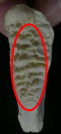
\includegraphics[scale = 0.75]{huesos/crestas_surcos_muy_definidos.png}  &   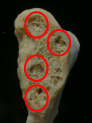
\includegraphics[scale = 0.75]{huesos/superficie_porosa_si.png} &  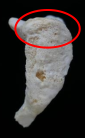
\includegraphics[scale = 0.75]{huesos/borde_superior_definido.png}  \\ \hline
	Nódulo óseo: Presente & Borde inferior: No definido & Borde dorsal: Definido \\ \hline
	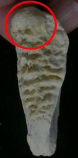
\includegraphics[scale = 0.75]{huesos/nodulo_oseo_presente.png} & 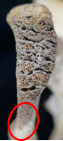
\includegraphics[scale = 0.75]{huesos/borde_inferior_no_definido.png} &  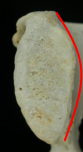
\includegraphics[scale = 0.75]{huesos/borde_dorsal_definido.png} \\ \hline
	Plataforma dorsal: Presente & Bisel ventral: En proceso de formación & Borde ventral: Muchas excrecencias \\ \hline
	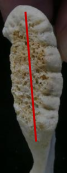
\includegraphics[scale = 0.75]{huesos/plataforma_dorsal_presente.png} & 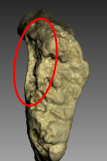
\includegraphics[scale = 0.75]{huesos/bisel_ventral_en_proceso_formacion.png} &   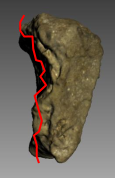
\includegraphics[scale = 0.75]{huesos/borde_ventral_muchas_excrecencias.png} \\ \hline
	\end{tabular}%
}
	\caption{Algunos ejemplos de las características consideradas por Todd.}\label{table:caracteristicas_todd}
\end{table}

Observando estas características Todd proponía una clasificación en diez fases:

\begin{itemize}
	\item Fase 1: 19 años.
	\item Fase 2: De 20 a 21 años.
	\item Fase 3: De 22 a 24 años.
	\item Fase 4: De 25 a 26 años.
	\item Fase 5: De 27 a 30 años.
	\item Fase 6: De 31 a 34 años.
	\item Fase 7: De 35 a 39 años.
	\item Fase 8: De 40 a 44 años.
	\item Fase 9: De 45 a 49 años.
	\item Fase 10: Más de 50 años.
\end{itemize}

Como era de esperar, podemos ver que las fases de edad más tempranas son más fáciles de asignar y los rangos de edad son más pequeños, mientras que en las fases más avanzadas los rangos de edad son mucho mayores, llegando a la última fase de más de 50 años, que aunque hoy en día nos parezca que gran parte de la población se asignaría a esa fase, en la época que Todd propuso esta clasificación la esperanza de vida era mucho menor.

En este problema se trata de un problema de clasificación ordinal, difícil de resolver debido a la complejidad en el conjunto de datos, además de requerir un modelo explicable de cara a ayudar a los expertos.

\subsubsection{Conjunto de datos}

Uno de los principales inconvenientes de este problema es que, como podemos ver, tenemos un gran número de características, de posibles valores para dichas características y de clases que asignar a cada dato, por lo que tendremos que buscar formas de tratar con la alta dimensionalidad del problema.

Por otro lado, es muy difícil obtener un buen conjunto de datos para este problema. En nuestro caso utilizaremos un conjunto de datos clasificado manualmente por el Laboratorio de Antropología Física de la Universidad de Granada\cite{laboratorioForenseUGR}.

Este conjunto está formado por datos tomados de ambas lateralidades de la sínfisis púbica, siendo en total 960 datos distribuidos en los diez rangos de edades propuestos por Todd.


\begin{figure}[H]
	\centering
	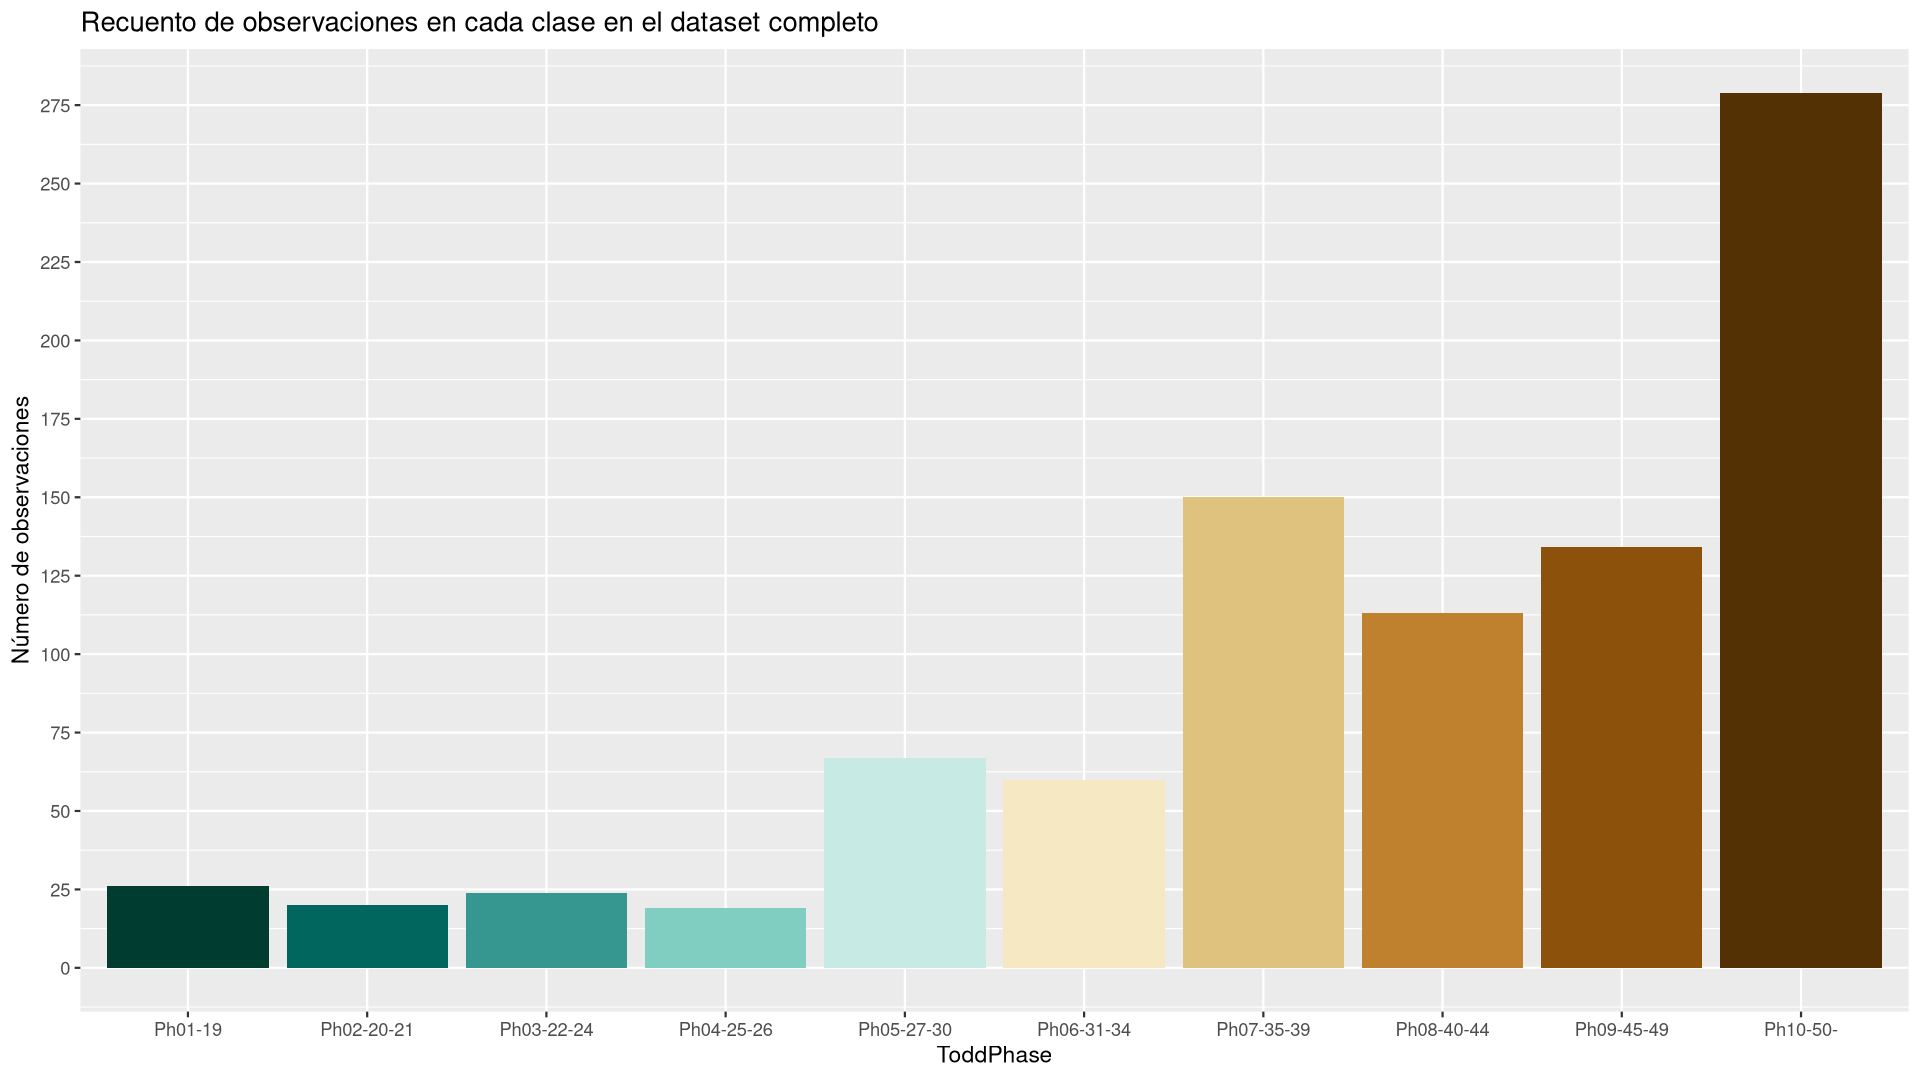
\includegraphics[width = \textwidth]{conjunto_datos/distribucion_clases_completo.png}
	\caption{Número de datos por cada fase propuesta por Todd con el conjunto de datos completo.}
	\label{fig:conteo_original}
\end{figure}


Como vemos, este conjunto de datos se encuentra claramente desbalanceado, hay muchas más muestras de las clases de edad más avanzada que de edades más bajas, además de contar con muy pocos en la mayoría de clases. Más adelante veremos como podemos solucionar estos problemas utilizando técnicas de sobremuestreo.

\subsection{Motivación}

Este trabajo está motivado porque la propuesta de Todd y sus trabajos derivados son demasiado subjetivos, haciendo muy poca distinción entre las fases y dejando gran parte del criterio de la estimación a cargo del forense.

Aunque en los últimos años se han desarrollado modelos de inteligencia artificial que son capaces de obtener buenos resultados en esta clase de problemas, los modelos actuales apenas son interpretables por los expertos y esto no les permite utilizarlos para avanzar en las técnicas de estimación de la edad a partir de restos óseos.

Por este motivo aparece la Inteligencia Artificial Explicable, y utilizando este tipo de técnicas intentaremos resolver el problema para que el experto sea capaz de entender y razonar como funciona el modelo.


\subsubsection{Inteligencia Artificial Explicable}

En la última década los distintos modelos de aprendizaje automático, como las redes neuronales, han revolucionado la inteligencia artificial. Estos nuevos modelos obtienen resultados impensables con modelos clásicos, aunque son demasiado complejos de interpretar. Por este motivo ha aparecido el concepto de Inteligencia Artificial Explicable \cite{XAI} (XAI de sus siglas en inglés).

La inteligencia artificial explicable trata de expresar modelos de inteligencia artificial de una forma simple e interpretable. Con esto se busca que no solo los desarrolladores de dichos modelos sean capaces de comprobar y validar como funciona el modelo, sino que los usuarios sean capaces de entender a grandes rasgos como funciona, ya que en muchas ocasiones han de ser capaces de interpretar las decisiones del modelo para realizar su trabajo.

En este trabajo, debido a la complejidad del problema, así como que el experto que utilizará los resultados del modelo ha de ser capaz de interpretar, validar, y tomar decisiones con los resultados del modelo, se buscará obtener un modelo simple y fácilmente interpretable. Por este motivo proponemos un sistema basado en reglas, donde se utilizará el algoritmo de Programación Genética para obtener el conjunto de reglas del sistema.

Por último, otro paradigma a integrar con la XAI cuando se dispone de conocimiento experto y teorías sobre el dominio del problema es la ciencia de datos guiada por teoría \cite{theoryGuidedDataScience}. La estructura del modelo XAI debe ser escogida acorde a las relaciones que pretendemos encontrar, y el conocimiento previo del problema puede aportar mucha información. Además, que el modelo tenga una salida interpretable ayuda a que el experto pueda revisar esa salida, y así descubrir nuevo conocimiento que pueda completar al actual.

La mayoría de los dominios de aplicación utilizados en problemas de ciencia de datos tienen un principio teórico clásico, subyacente a la aplicación o contexto donde se producen los datos del problema. Este principio teórico se usa habitualmente como conocimiento previo por los expertos, y se puede usar en XAI para mejorar los modelos, ya que los datos deben estar correlacionados con los principios teóricos del problema.

\newpage

\subsection{Objetivos}

Tras introducir el problema, comentar los principales retos que nos podemos encontrar y orientar que tipo de solución buscamos, podemos distinguir estos claros objetivos:

\begin{enumerate}
	\item Discutir la importancia de resolver este problema, así como los distintos enfoques utilizados hasta ahora en los diferentes estudios que se han propuesto resolverlo.
	\item Estudiar y discutir distintos métodos de preprocesamiento de datos, en especial el balanceado de datos debido a las características del problema.
	\item Estudiar, desarrollar y entrenar algoritmos evolutivos que permitan inferir reglas a partir de un conjunto de datos, discutiendo y analizando las distintas técnicas utilizadas hasta el momento para esta tarea.
	\item Implementar un sistema basado en reglas capaz de resolver el problema.
	\item Estudiar la idoneidad de la solución propuesta para el problema teniendo en cuenta tanto su factor de acierto como su interpretabilidad de cara a ser usado por expertos en el problema.
\end{enumerate}


\newpage


\section{Estado del arte y antecedentes}

\subsection{Estado del arte del problema a tratar} \label{sec_estado_arte_problema}

El problema de la estimación de la edad a partir de restos óseos ya se ha tratado en distintas ocasiones, desde modificaciones a la propuesta de Todd, propuestas de como automatizar la estimación utilizando las características que proponía Todd, hasta estudios que utilizaban técnicas de visión por computador para recoger y procesar las características de los restos.

En 1990, J. M. Suchey y S. Brooks propusieron una modificación a la propuesta de Todd \cite{sucheyBrooks}, en la que evaluaban $739$ restos óseos y llegaban a la conclusión de que era posible reducir las diez fases propuestas por Todd a seis fases, modificando el criterio de cada una de las fases y añadiendo cierto error marginal, aunque con un $95\%$ de confianza con los nuevos intervalos propuestos. Esta modificación es una de las más aceptadas por la comunidad científica, aunque la mayor parte de trabajos siguen utilizando las fases propuestas por Todd.

% TODO buscar estado del arte enfocado a clasificación a sistemas basados en reglas

Uno de los más relevantes es un estudio publicado en el año 2015 en la revista \textit{Journal of forensic sciences} \cite{modelandoHuesos3D}, en el que se escaneaban los restos tomados como muestras para la variación de la sínfisis púbica y con esta variación realizar la estimación de la edad utilizando un modelo de regresión lineal y las seis fases propuestas por Suchey y Brooks. El conjunto de datos utilizado en este experimento se compone de $41$ esqueletos de personas estadounidenses y logran obtener una raíz del error cuadrático medio de unos $17.15$ años.

\begin{figure}[H]
	\centering
	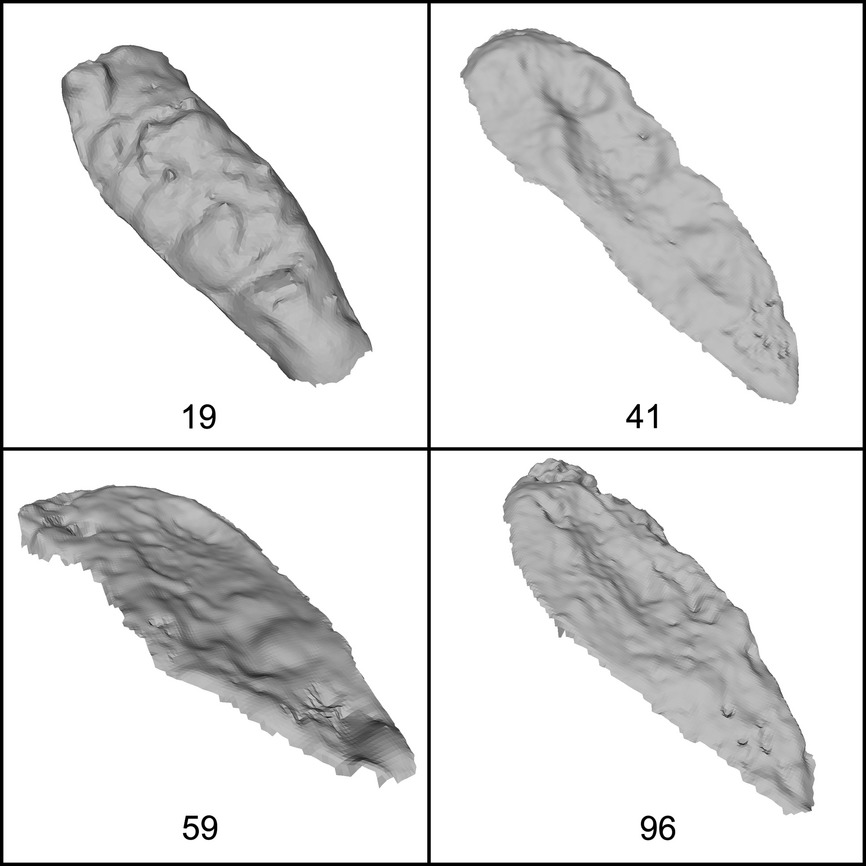
\includegraphics[scale = 0.4]{escaneo_huesos.jpg}
	\caption{Visualización del escaneo de la sínfisis púbica en cuatro individuos. La edad de la muerte aparece en la parte inferior de cada imagen. Imagen obtenida de \cite{modelandoHuesos3D}.}
	\label{fig:escaneo_huesos}
\end{figure}

Ese mismo año, los mismos autores presentaron una mejora \cite{mejoraModelandoHuesos3D} en la que, en lugar de utilizar la variación total de la sínfisis púbica, utilizaban la flexión de un plano de forma que dicho plano coincida con la superficie del hueso. De esta forma, utilizando un conjunto de datos similar a su experimento anterior y la curvatura de la sínfisis púbica entrenaron un modelo de regresión lineal con el que obtuvieron una raíz del error cuadrático medio de unos $19$ años.

A finales de 2015, Beatrix Dudzik y Natalie R. Langley, de la Universidad de Tennessee y la Universidad Lincoln Memorial, propusieron \cite{componentBased} varios modelos basados en árboles de decisión y regresión logística multinomial. Para estos experimentos utilizaron 5 características de la sínfisis púbica de 47 individuos de entre 18 y 40 años. Obtuvieron muy buenos resultados, con una tasa de acierto del $94\%$ aunque solo utilizaban 3 de las 6 fases propuestas por Suchey y Brooks.

\begin{figure}[H]
	\centering
	\begin{subfigure}{.5\textwidth}
	  \centering
	  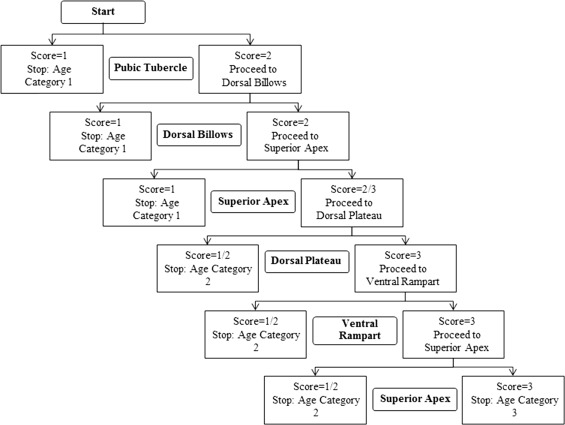
\includegraphics[scale = 0.7]{cita_7_arbol.jpg}
	  \caption{Árbol de decisión implementado en \cite{componentBased}}
	  \label{fig:arbol_c7}
	\end{subfigure}%
	\begin{subfigure}{.5\textwidth}
	  \centering
	  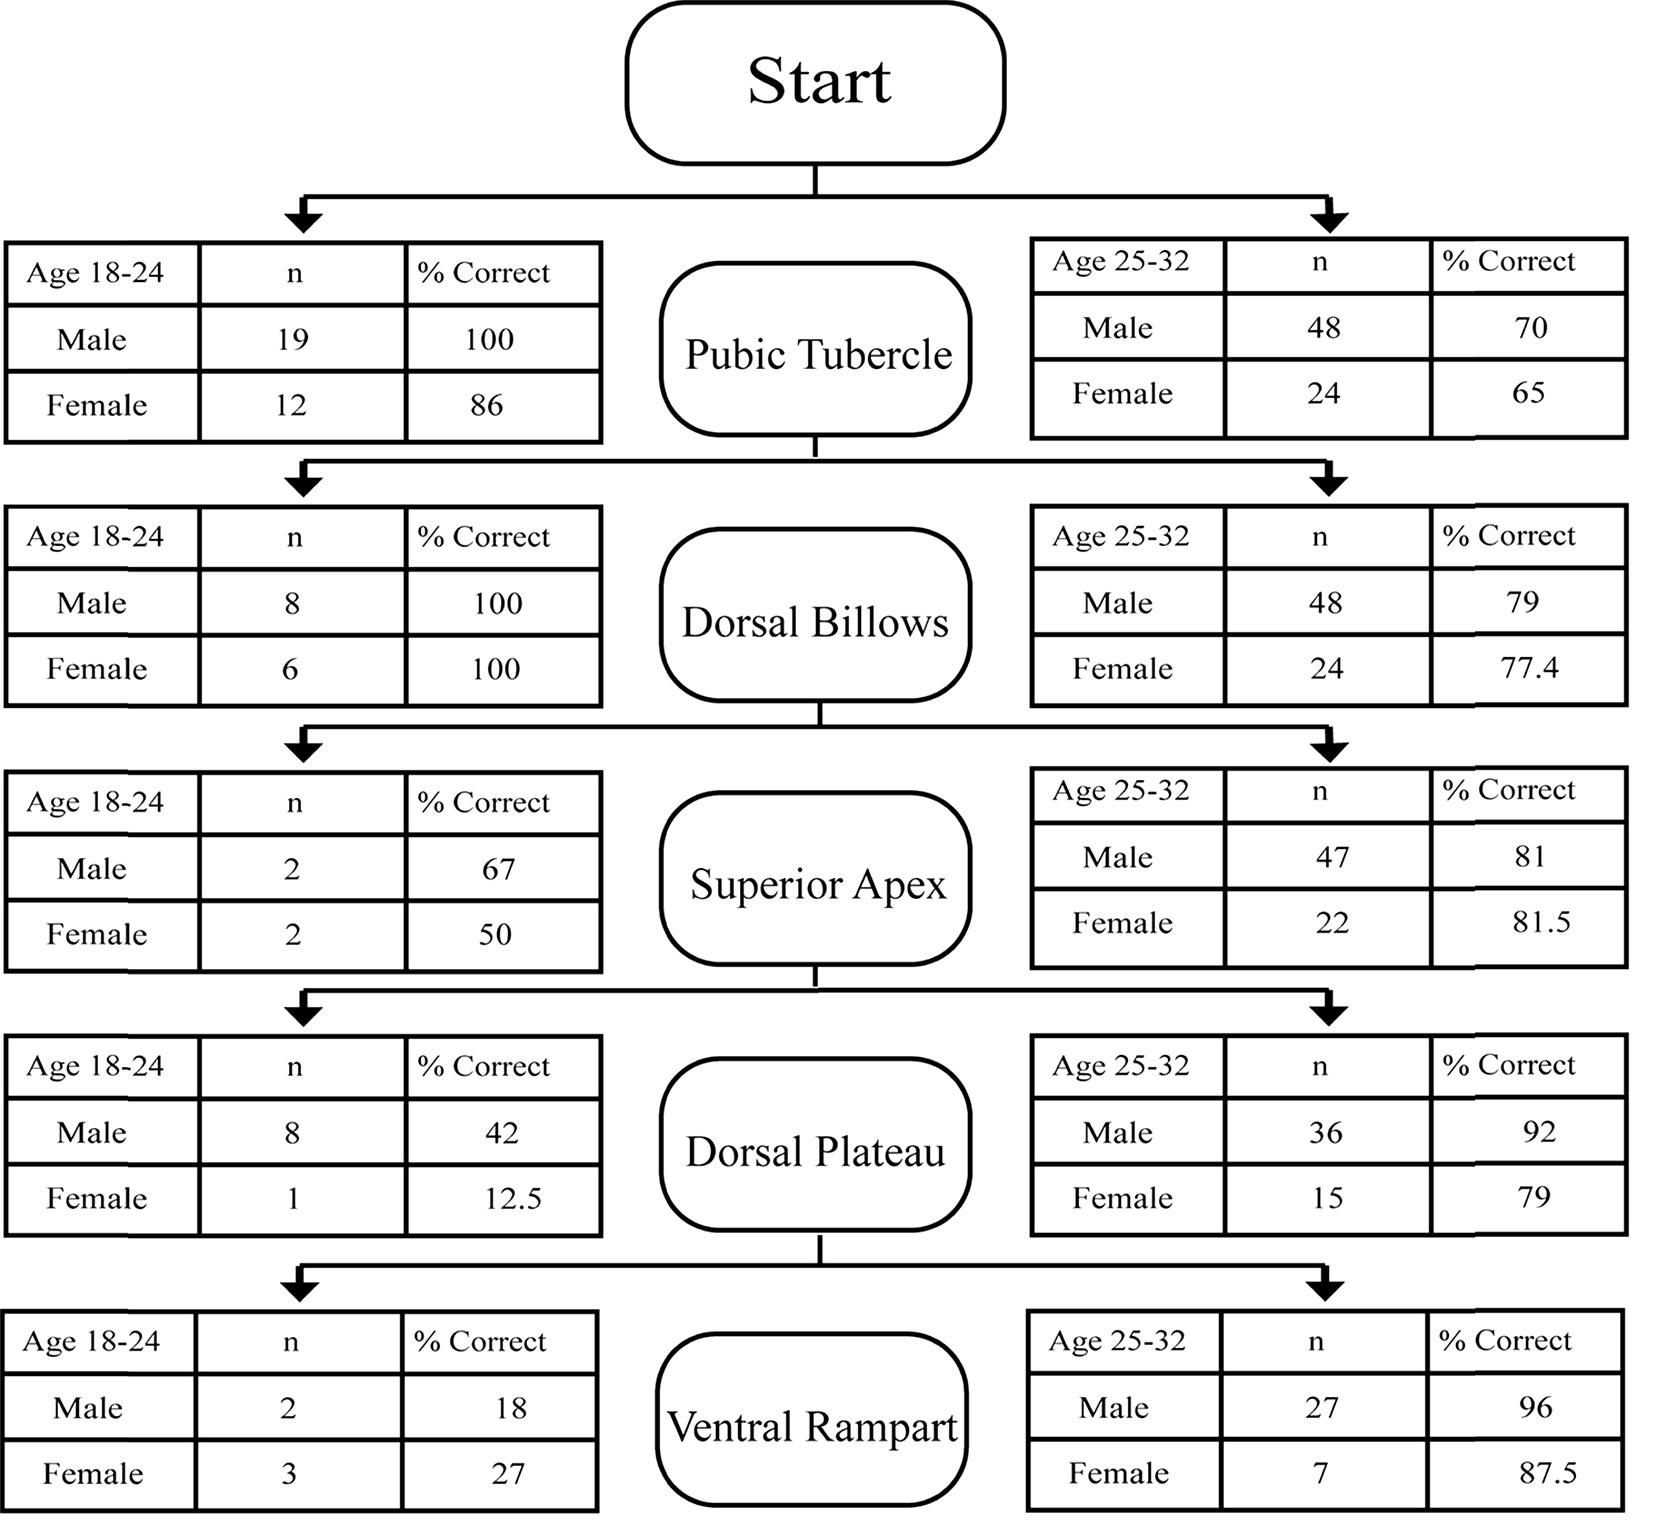
\includegraphics[scale = 0.8]{cita_7_ejemplo_dos_fases.jpg}
	  \caption{Porcentaje de acierto para la fase 1 y 2 de \cite{componentBased}.}
	  \label{fig:acierto_cita7}
	\end{subfigure}
	\caption{Imágenes obtenidas de \cite{componentBased}.}
	\label{fig:arboles_cita7}
\end{figure}



Más adelante, en 2018, varios investigadores de la República Checa publicaron un trabajo \cite{estimacionHuesosCadera} en el que, con un conjunto de $941$ restos óseos de personas de distinta raza entre 19 y 100 años, utilizando datos de los huesos de la cadera estudiaban las características comunes y las que diferenciaban las distintas edades, y consideraban 9 modelos distintos para realizar una estimación, desde un sistema de puntuación tradicional, utilizando la variación entre los huesos, distintos de regresión lineal, árboles de decisiones o redes neuronales artificiales. De estos modelos se llega a la conclusión que el mejor es un modelo de regresión multinomial, con el que obtienen una raíz del error cuadrático medio de unos $12.5$ años.

En 2017 investigadores de la Universidad de Granada publicaron un artículo preliminar de cara a obtener un modelo descriptivo basado en reglas con el que realizar la estimación de la edad a partir de la sínfisis púbica \cite{fuzzyAgeEstimation}. Utilizando $74$ muestras clasificadas manualmente consiguen entre 17 y 20 reglas utilizando árboles de decisión difusos que consiguen un error absoluto medio de $1.68$ años, aunque el resultado no es totalmente fiable debido a que no consiguen reglas para algunas fases propuestas por Todd.

Más adelante, en 2021, este mismo equipo con la ayuda de investigadores de la Universidad de Cordoba publicaron una continuación de su estudio \cite{NSLVOrdAge}. En este caso, utilizando el mismo conjunto de datos que utilizaremos nosotros, aplicando técnicas de balanceo y sobremuestreo de datos para resolver problemas relativos a dicho conjunto de datos, han enfocado el problema como un problema de clasificación ordinal. Utilizando el software NSLVOrd \cite{NSLVOrd}, un algoritmo de clasificación ordinal basado en el enfoque de aprendizaje de reglas de forma iterativa publicado por investigadores de la Universidad de Granada en 2016, son capaces de obtener una raíz del error cuadrático medio de $12.34$ años utilizando 34 reglas para las distintas fases. Este es, hasta este momento, el mejor resultado del estado del arte de este problema, y además en este estudio se discute sobre la importancia de las características a observar en la sínfisis púbica propuestas por Todd, llegando a la conclusión de que ciertas características nunca se utilizan, y por lo tanto no entran en juego a la hora de realizar la estimación de la edad.


% Comentar el enfoque de Gilbert y McKern y diferenciar ambos enfoques

Otro enfoque de este problema es el propuesto por McKern y Stewart en el año 1957 \cite{primeraPropuestaMcKern} y que luego ampliarían en 1973 junto a Gilbert \cite{propuestaGilbert}. En lugar de resolver el problema con un enfoque de clasificación, proponían un método en el que se le asignan valores numéricos a cada uno de los distintos posibles estados de cada característica observada en la sínfisis púbica, y con esos valores conseguir una fórmula que estimase la edad. En este trabajo utilizaremos este enfoque de cara a tratar este problema como un problema de regresión. En la siguiente sección haremos una presentación más detallada de este método.

Uno de los primeros trabajos que aplico este enfoque fue un estudio de la Universidad de Tokio \cite{primerTrabajoGilbert}. Los autores utilizan una extensión de la regresión lineal, regresión lineal múltiple, ya que utilizan siete características de la sínfisis púbica y una constante de cara a obtener fórmula que les sea capaz de estimar la edad. Tras los distintos experimentos, consiguen obtener unos resultados bastante buenos aunque, como los propios autores indican, el rango de edades con el que se ha trabajado es bastante limitado, siendo solo entre 18 y 38 años y solo contando con 135 muestras de sínfisis púbica.

Años más tarde, en 1995, Investigadores del departamento de Medicina Forense del All India Institute of Medical Sciences en Nueva Delhi, India, utilizarán este trabajo para aplicarlo a 41 individuos de entre doce y setenta y cinco años, comparando los resultados utilizando regresión lineal múltiple con el sistema de clasificación de Todd \cite{estudioComparandoGilbertTodd}. En este trabajo se logran obtener resultados significativamente mejores que con la propuesta de Todd, además de sumarse a las conclusiones de otros trabajos, que aunque tomen un enfoque distinto, se podrían modificar las fases propuestas por Todd, ya que se observan como algunas de las variables tienden a zonas entre dos fases de Todd, además de encontrar algunas de las características de la sínfisis púbica irrelevantes a la hora de estimar la edad en muchas de las fases.



\subsection{Sistemas basados en reglas}

%  TODO : Redactar esta sección para explicar en que se ha utilizado principalmente sistemas basados en reglas,
% cuando aparecieron, etc, etc

\subsection{Programación Genética}

La Programación Genética apareció como una adaptación de los algoritmos evolutivos para representar programas de ordenador como cromosomas en una estructura de árbol. A pesar de que su aparición fue en 1985 no fue hasta principios de 1990 cuando este método comenzó a ser más utilizado gracias a John Koza \cite{kozaGP}.

La forma en la que la Programación Genética expresa los cromosomas permite resolver problemas de distintos tipos dando soluciones sencillas de interpretar, por este motivo este algoritmo y sus variaciones han sido bastante utilizadas.

Uno de los primeros trabajos fue de publicado por P. A. Whigham en 1995 \cite{PGgramaticas}, en el que se utiliza una gramática inicial libre del contexto para generar expresiones a utilizar en el algoritmo, y que durante el entrenamiento el algoritmo complete la gramática y la amplíe con nuevas reglas, siendo un claro ejemplo de aprendizaje incremental.

% TODO: Modificar esta parte para comentar que se puede usar para aprender un sistema basado en reglas,
% que es el objetivo del TFM
Tras demostrar la potencia de Programación Genética para aprender estructuras gramaticales, una de sus principales aplicaciones fue sistemas basados en reglas, donde se utilizaban algoritmos evolutivos para aprender las reglas del sistema.

En 1996, Edward Tunstel, investigador de la NASA y Mo Jamshidi, investigador de la Universidad de Nuevo México, publicaron un artículo \cite{PGcontrolRobots} en el que utilizaban sistemas basados en reglas difusas para un sistema de control de un robot en un entorno tridimensional, donde se utilizaba Programación Genética para el aprendizaje de las reglas del sistema, aprovechando la estructura de gramática de los individuos de la población. Utilizando tan solo poblaciones de entre diez y veinte reglas, escogiendo la regla con mejor ajuste, y con doce ejecuciones del algoritmo, obtuvieron doce reglas capaces de resolver el problema.

\begin{figure}[H]
	\centering
	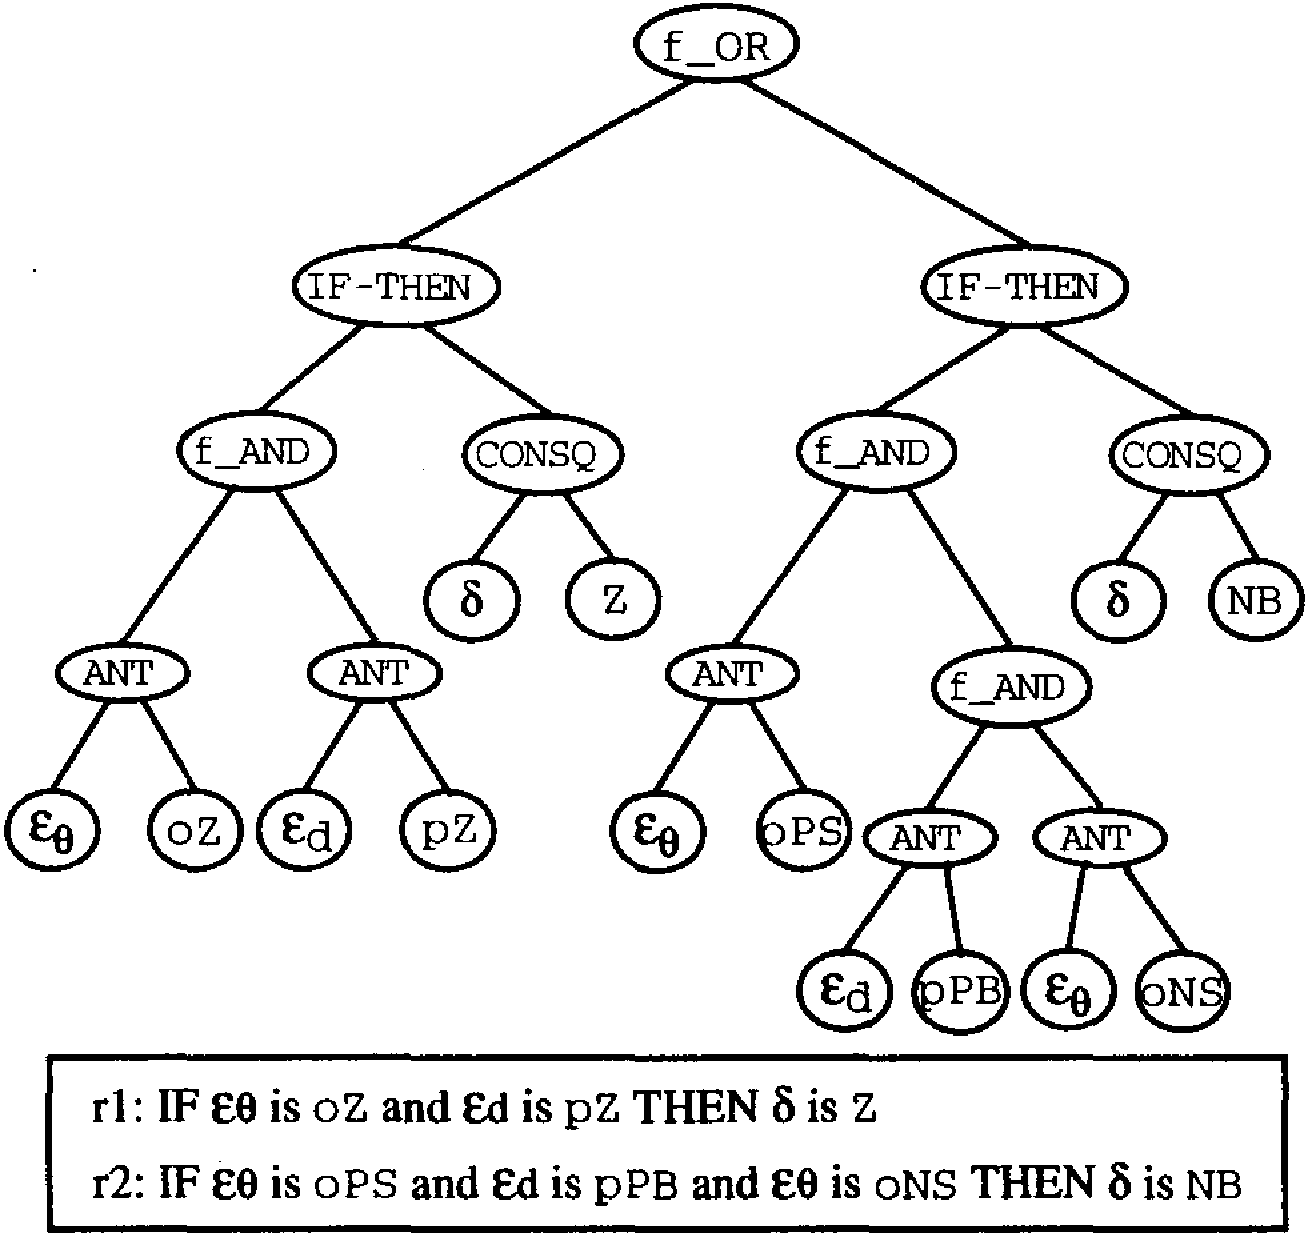
\includegraphics[width = 0.5\textwidth]{imagenes_papers/imagen_arbol_regla_robots.png}
	\caption{Ejemplo de regla difusa representada como un árbol del trabajo \cite{PGcontrolRobots}.}
	\label{fig:imagen_arbol_regla_robots}
\end{figure}

Más adelante, en el año 2000, investigadores del Centro Federal de Educación Tecnológica de Paraná, en Brasil, desarrollaron un trabajo \cite{trabajoChestPain} bastante similar al problema propuesto debido a la alta cantidad de clases y las pocas observaciones del problema disponibles. En este trabajo proponen un sistema basado en reglas de cara a predecir diagnósticos de doce tipos distintos de dolor torácico. De cara a obtener las reglas necesarias utilizan Programación Genética, lanzando para cada clase diez ejecuciones del algoritmo, manteniendo la mejor regla para cada clase como resultado, obteniendo un total de doce reglas. A pesar del bajo número de observaciones, consiguen unos resultados muy altos tanto de sensibilidad (probabilidad de detectar los verdaderos positivos) como de especificidad (probabilidad de detectar los verdaderos negativos), además de una simplicidad de las reglas (valor obtenido a partir del número máximo de nodos y el número de nodos de cada regla) muy cercanos a uno, mostrando la clara ventaja de sistemas basados en reglas para obtener modelos explicables.

Otro trabajo interesante es el publicado por Tsakonas et al en 2004 \cite{reglasDosDominiosMedicosComparacion} donde se proponen evaluar la potencia de Propagación Genética en dos problemas médicos, así como comparar los resultados con otros métodos como árboles C4.5. Para el primer problema se obtienen resultados con alrededor de un 70\% de acierto utilizando C4.5, utilizando Programación Genética para regresión simbólica se consigue un acierto cercano al 90\%, mientras que con Programación Genética obteniendo un sistema basado en reglas se consigue un acierto algo superior al 85\%. Para el segundo problema C4.5 consigue un acierto del 70\%, mientras que Programación Genética consigue alrededor de un 98\% con las distintas variantes.


Otro de sus principales usos es regresión simbólica, ya que nos ofrece un algoritmo muy bueno para problemas en los que los resultados son variables, no se conoce a priori la forma que tendrá el resultado, además de todas las ventajas de los algoritmos evolutivos.

La principal forma de conseguir que Programación Genética trabaje con regresión simbólica es modificar los cromosomas propuestos por John Koza, en lugar de ser programas de ordenador, generador por gramáticas, los cromosomas serán expresiones matemáticas, manteniendo siempre la forma de árbol. Esta modificación es tan simple por reemplazar la gramática por una gramática que genere expresiones matemáticas, con los operadores que se estimen oportunos.

En 1995, investigadores de la Universidad de Georgia publicaban un artículo \cite{primerGAP} en el que proponían utilizar Programación Genética para hacer regresión simbólica, es decir, aprender una fórmula matemática estructurada como un árbol. En este trabajo se mencionan los principales problemas de la Programación Genética para regresión simbólica, todos ellos derivados de que este algoritmo solo puede modificar la estructura de las expresiones, no su contenido como tal, no siendo capaz de trabajar con valores numéricos constantes, además de generar ramificaciones complejas para obtener cierta constante. En este trabajo se propone añadir un algoritmo genético a Programación Genética de cara a resolver estos problemas aprendiendo las constantes numéricas en un cromosoma independiente, de ahí el nombre GA-P (Genetic Algorithm-Programming).

Más adelante esta variación de Programación Genética se utilizará en diversos trabajos, como el publicado por investigadores de la Universidad de Oviedo y la Universidad de Granada en 1999 \cite{GAPredElectrica}, donde utilizando este algoritmo consiguen unos resultados bastante buenos en dos problemas reales aplicando regresión simbólica, el trabajo del año 2000 de los investigadores del Laboratorio Nacional de Computación Científica de Brasil, donde publican un artículo \cite{PGregresionSimbolica} donde explican y proponen en detalle los distintos operadores necesarios para GA-P, así como otro trabajo del año 2000 en el que investigadores de la Universidad de Granada utilizan GA-P para aprender consultas booleanas \cite{GAPFormulasBooleanas} en el que demuestran la versatilidad del algoritmo para distintos problemas además de obtener soluciones fácilmente interpretables.



\newpage


\section{Propuesta}

\subsection{Conjunto de datos a utilizar}

Para realizar este trabajo utilizaremos un conjunto de datos con $892$ muestras de la sínfisis púbica clasificados manualmente por investigadores del Laboratorio de Antropología Física de la Universidad de Granada utilizando las diez fases propuestas por Todd.

Este conjunto de datos se divide en dos partes, las muestras tomadas de la lateralidad izquierda ($439$ muestras) y la lateralidad derecha ($453$ muestras) del pubis.

\subsubsection{Problema del balanceo de clases}

Como vimos en la figura \ref{fig:conteo_original} con el conteo de cada una de las fases en el conjunto completo, los datos de este problema se encuentran altamente desbalanceados, hay rangos de edades en las que apenas contamos con datos, y la diferencia entre número de datos entre una edad temprana y alta es muy grande. De cara a resolver este problema proponemos utilizar un algoritmo de sobremuestreo de datos, al igual que \cite{NSLVOrdAge}.

En este artículo se proponen distintas técnicas de sobremuestreo, principalmente utilizando un sobremuestreo de forma aleatoria, utilizando el algoritmo SMOTE \cite{revisionSMOTE} (y varias variaciones de este algoritmo), y utilizando el algoritmo ADASYN \cite{propuestaADASYN}.

En nuestro caso, al utilizar el mismo conjunto de datos, podemos ver en su artículo que la técnica que mejor ha funcionado para este conjunto de datos es Borderline-SMOTE, así que también utilizaremos esta técnica aunque tendremos en cuenta otras para comprobar si con nuestro enfoque otras técnicas permiten mejorar los resultados del modelo.

\subsubsection{Enfoque con el que trabajaremos el conjunto de datos}


\begin{figure}[H]
    \centering
	  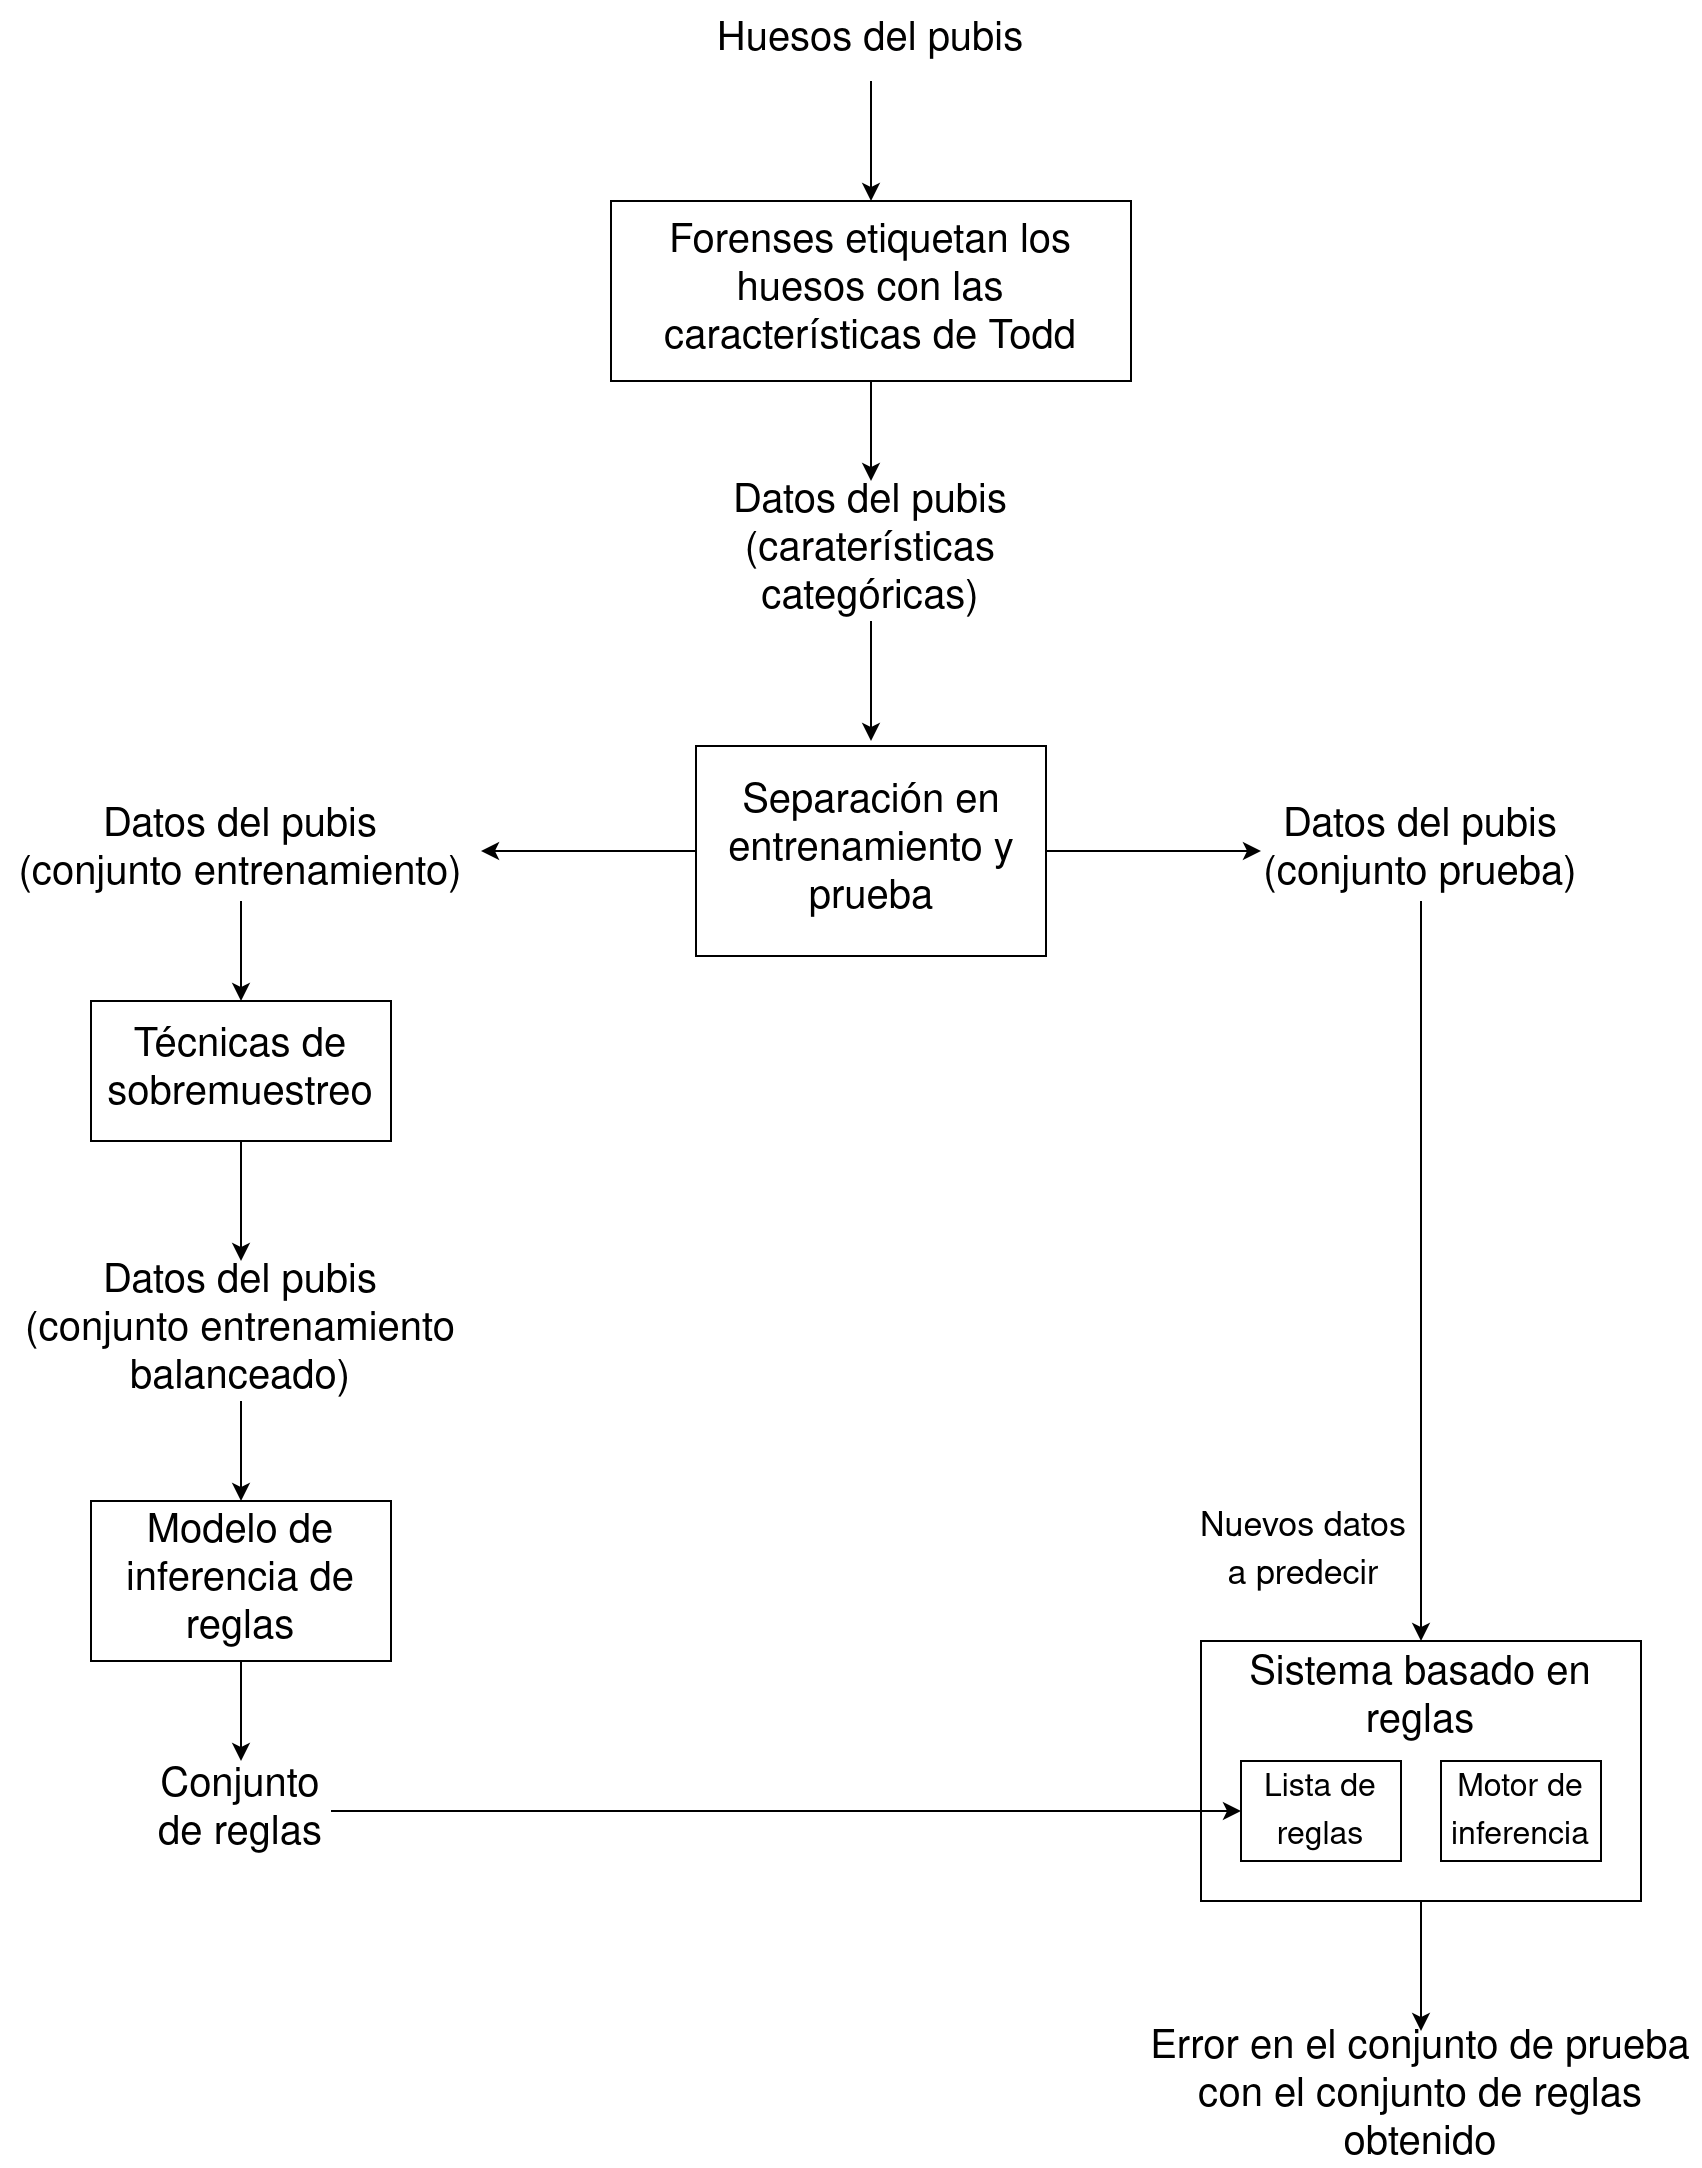
\includegraphics[width=0.8\textwidth]{esquema_datos.png}
    \caption{Esquema general de los pasos que seguirá el conjunto de datos para entrenar y validar el modelo.}
	 \label{fig:esquema_datos}
\end{figure}

En la figura \ref{fig:esquema_datos} podemos ver el flujo que seguirán los datos de entrada, a falta de concretar el sistema de validación a utilizar, 5x2cv, que se explicará más adelante.

\newpage

\subsection{Algoritmos a utilizar e implementación}

De cara a la implementación se propone utilizar \textit{R} para realizar el análisis de los datos debido a la gran cantidad de bibliotecas y herramientas que ofrece, \textit{Python} para aplicar parte del preprocesado de los datos ya que este lenguaje cuenta con múltiples herramientas para análisis de datos así como muchos de los métodos que vamos a utilizar, mientras que para la implementación de los algoritmos evolutivos se utilizará \textit{C++}.

La decisión de utilizar \textit{C++} viene dada ya que estos algoritmos tienden a ser lentos a la hora de realizar su entrenamiento, por lo que se ha buscado un lenguaje compilado con el que tener mejores tiempos de ejecución. También nos permite realizar una implementación orientada a objetos, lo que nos dará una mejor estructura del código a implementar, así como utilizar software como \textit{OpenMP} \cite{OpenMP} de cara a paralelizar secciones de código que nos permiten reducir el tiempo de ejecución gracias al paralelismo de datos, como veremos más adelante.

Por último, este lenguaje nos ofrece distintas herramientas de control del software, como \textit{GDB} \cite{gdb} para depurar el código, \textit{Valgrind} \cite{valgrind} para comprobar que no existen problemas con la memoria dinámica y la biblioteca \textit{Google Test} \cite{gtest} para realizar test unitarios y comprobar que el código funciona correctamente.

También se utilizará el sistema de control de versiones \textit{Git} \cite{git} durante todo el proceso de creación del código y esta memoria.

% TODO plantear ir añadiendo una planificación temporal

% \subsection{Planificación temporal}

\newpage


\section{Análisis y preprocesado de los datos}

\subsection{Análisis del conjunto de datos}

Nuestro conjunto de datos se compone de tres ficheros:

\begin{enumerate}
	\item \texttt{lateralidad0.arff} : 439 muestras de la lateralidad izquierda del pubis.
	\item \texttt{lateralidad1.arff} : 453 muestras de la lateralidad derecha del pubis.
	\item \texttt{completo.arff} : 892 muestas de ambas lateralidades, se compone de los dos ficheros antes en conjunto.
\end{enumerate}

\begin{figure}[H]
	\begin{lstlisting}[language={}]
	NoGrooves,Absence,Defined,Absent,Defined,Present,Absent,Absent,FormedWithoutRarefactions,Ph07-35-39
	\end{lstlisting}
	\caption{Ejemplo de un dato cuya edad de muerte está en el rango comprendido por la fase 7, entre 35 y 39 años, del conjunto de datos \texttt{completo.arff}.}
	\label{fig:ejemplo_dato}
\end{figure}

Como vemos en la figura \ref{fig:ejemplo_dato} los datos tienen asignados valores categóricos para cada característica, y finalmente la edad a la que murió la persona con las características asociadas.

Para comenzar, realizaremos un análisis de cada uno de los conjuntos de datos. Como el conjunto de datos completo se trata simplemente de la unión de los datos de la lateralizad izquierda y la derecha, será el último análisis que realicemos.

\subsubsection{Análisis de la lateralidad izquierda}

Este conjunto de datos cuenta con 439 muestras. Vamos a ver de forma gráfica como se distribuyen los datos según las fases propuestas por Todd, comentando la información que nos puede ser de utilidad de cada gráfico:

\begin{figure}[H]
	\centering
	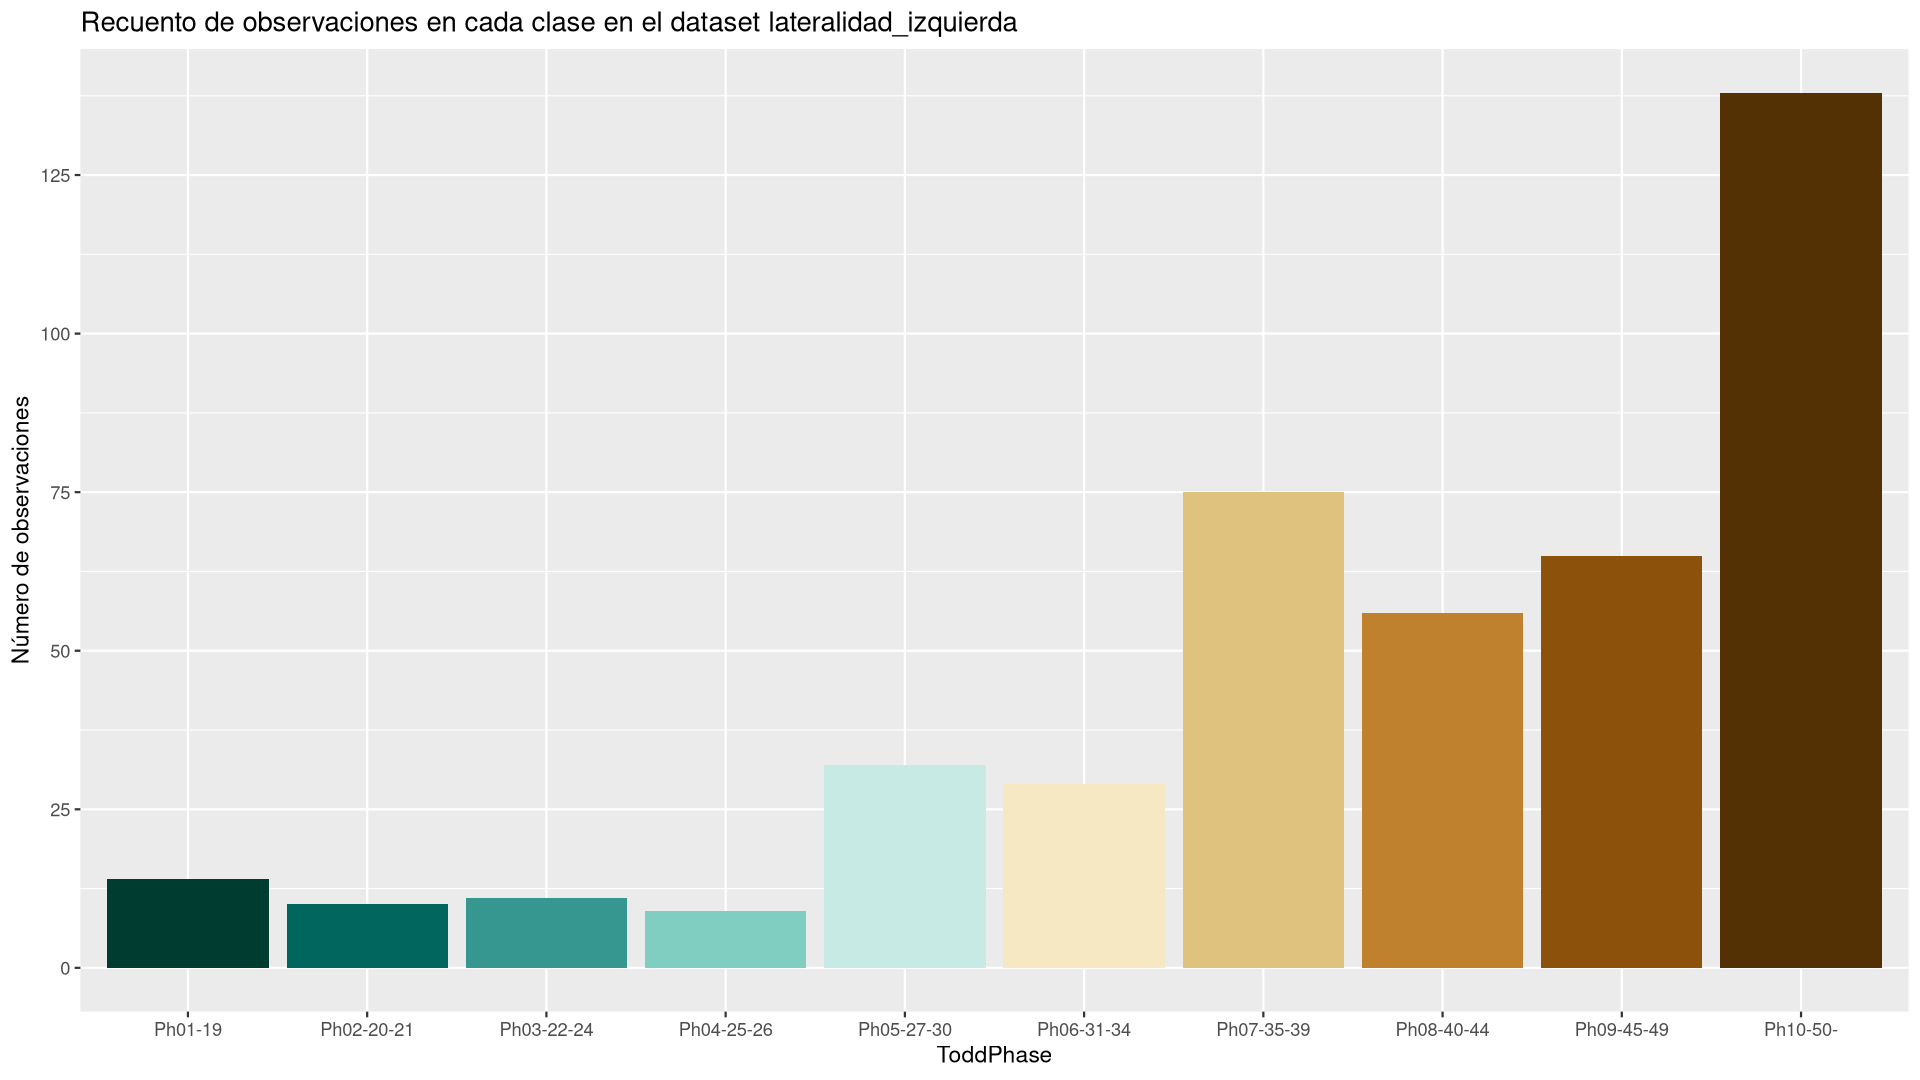
\includegraphics[width = \textwidth]{conjunto_datos/distribucion_clases_lateralidad_izquierda.png}
	\caption{Número de datos por cada fase propuesta por Todd con el conjunto de datos de la lateralidad izquierda.}
	\label{fig:conteo_l0}
\end{figure}

Podemos ver que contamos con una cantidad muy alta de observaciones de las últimas fases en comparación con las primeras fases, en especial de la última fase, de personas de más de cincuenta años.

Debido a que todas las variables del conjunto de datos son categóricas, para este análisis solo podemos observar como se distribuyen los valores de cada predictor para cada fase. Vamos ver cada uno de estos predictores y comentar la información que nos proporcionan.

\begin{figure}[H]
	\centering
	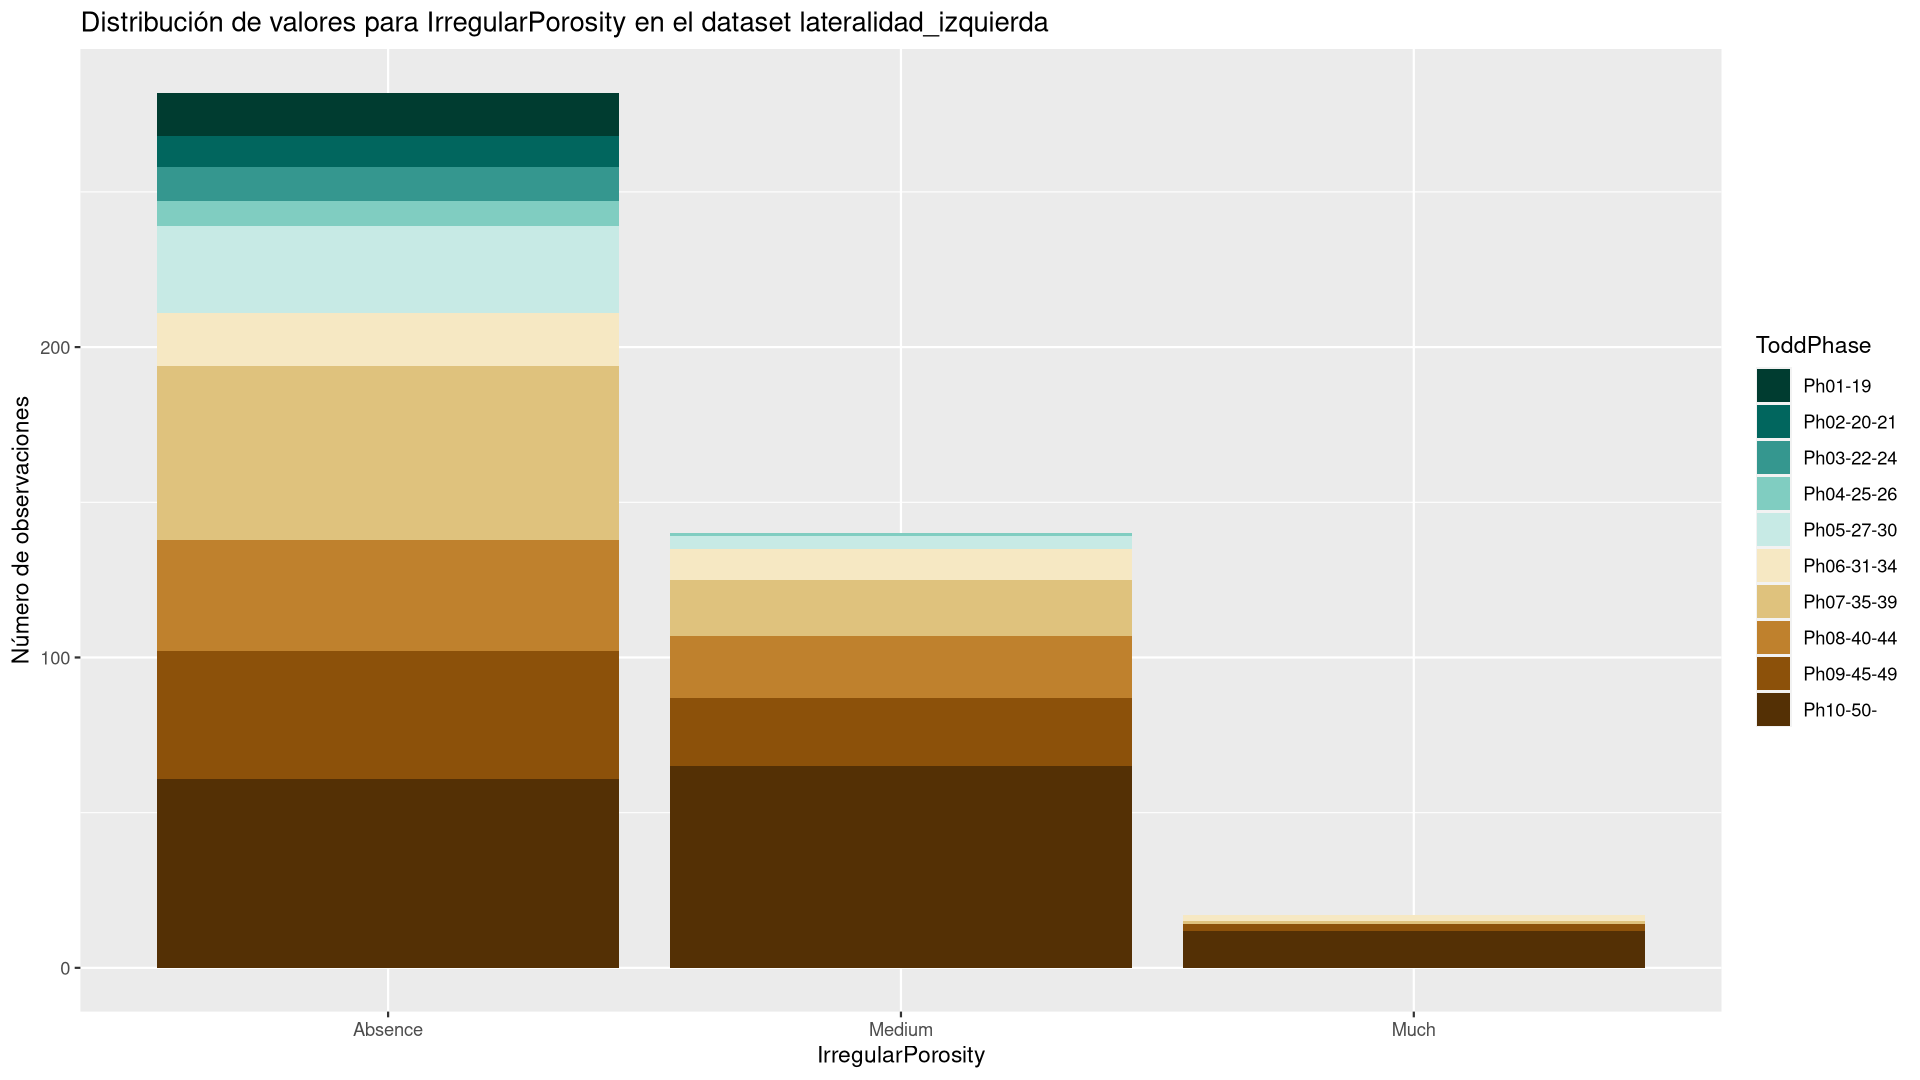
\includegraphics[width = \textwidth]{conjunto_datos/densidad_IrregularPorosity_lateralidad_izquierda.png}
	\caption{Distribución de los valores de IrregularPorosity en el conjunto de datos de la lateralidad izquierda.}
	\label{fig:densidad_IrregularPorosity_lateralidad_izquierda}
\end{figure}

En la figura \ref{fig:densidad_IrregularPorosity_lateralidad_izquierda} podemos observar la distribución de valores de \texttt{IrregularPorosity}. En este vemos como claramente con esta característica podremos clasificar observaciones de clases altas si el valor de esta variable es \texttt{Much}, mientras que con el valor \texttt{Medium} y en especial \texttt{Absence} si hay un mayor solapamiento entre las clases.

Aun así, podemos ver como esta característica tampoco nos aporta gran información para las fases más bajas, donde si se solapa este valor. Vamos a seguir observando el resto de predictores.

\begin{figure}[H]
	\centering
	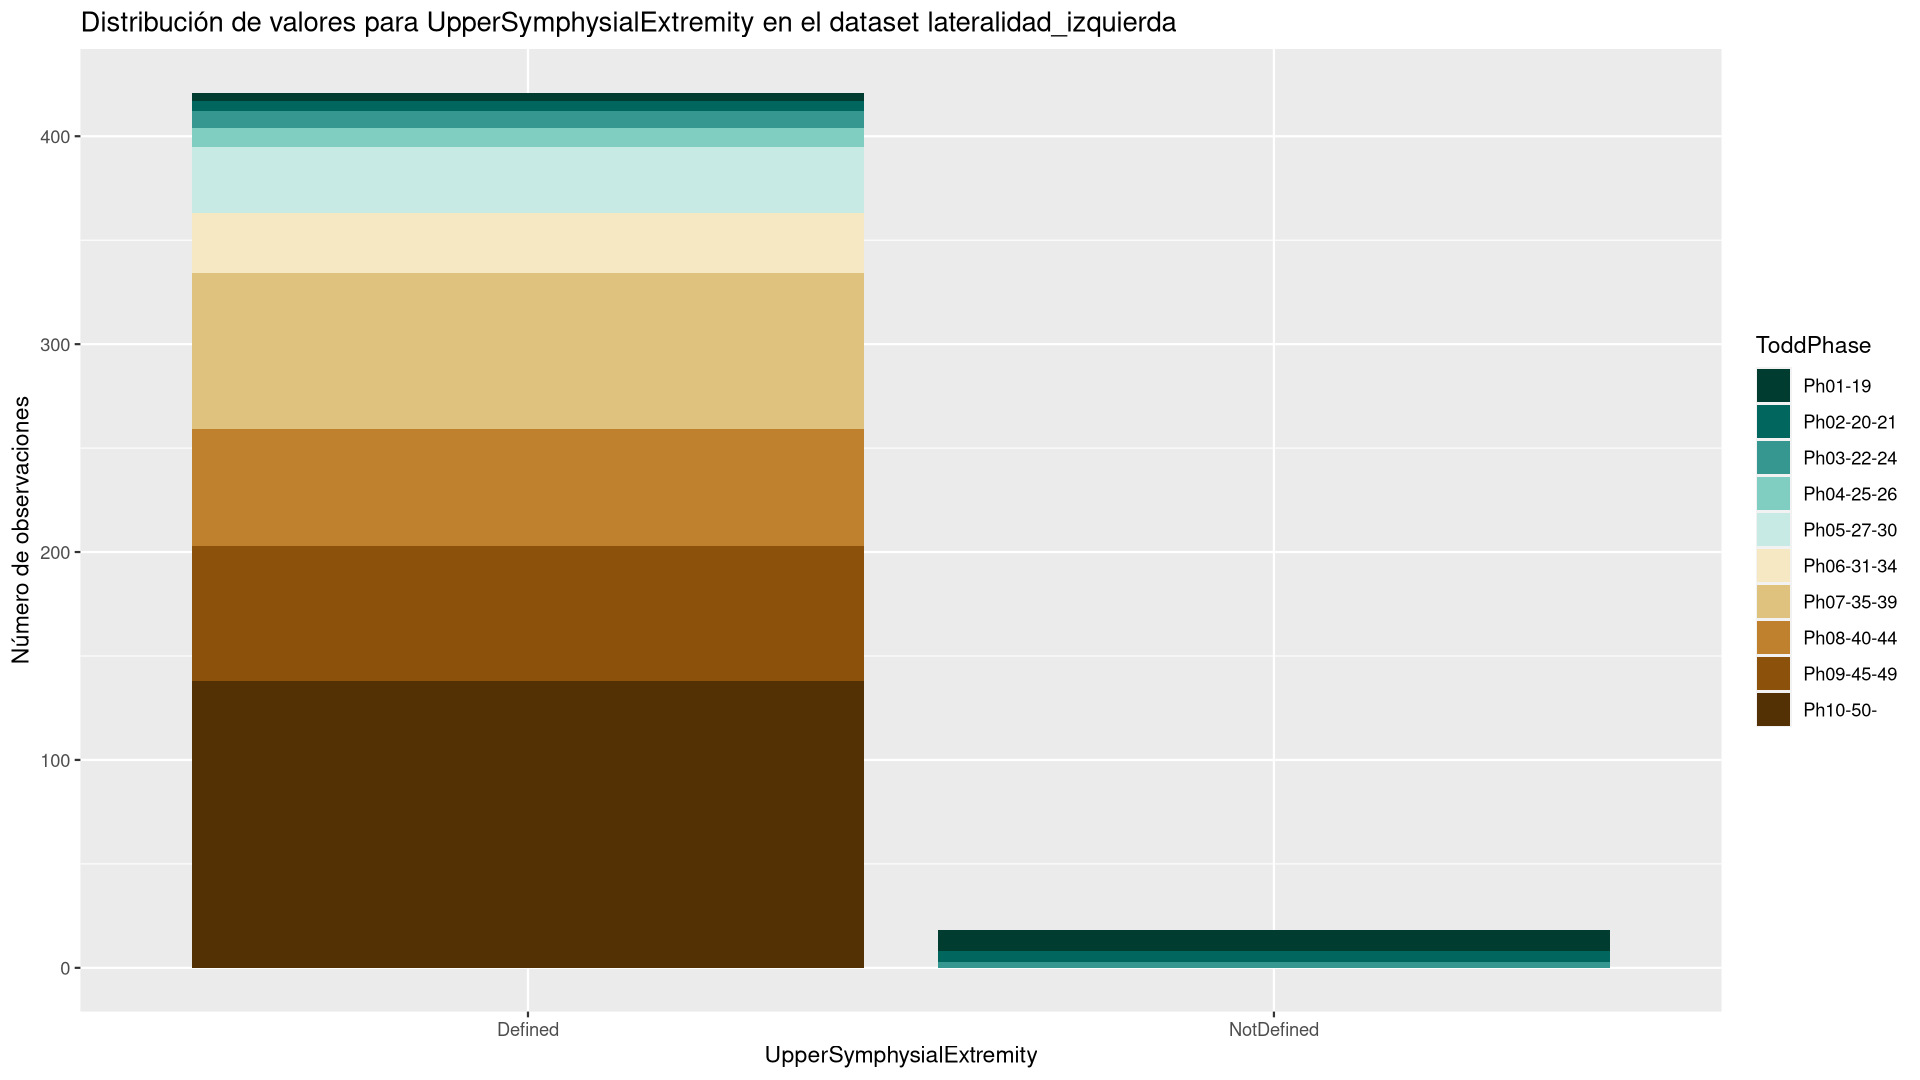
\includegraphics[width = \textwidth]{conjunto_datos/densidad_UpperSymphysialExtremity_lateralidad_izquierda.png}
	\caption{Distribución de los valores de UpperSymphysialExtremity en el conjunto de datos de la lateralidad izquierda.}
	\label{fig:densidad_UpperSymphysialExtremity_lateralidad_izquierda}
\end{figure}

En este caso con \texttt{UpperSymphysialExtremity}, como vemos en la figura \ref{fig:densidad_UpperSymphysialExtremity_lateralidad_izquierda}, ocurre lo contrario que en el caso anterior. Esta característica nos podría servir muy bien para predecir asegurarnos que estamos ante observaciones de fases bajas si toma el valor de \texttt{NotDefined}, sin embargo vemos como las observaciones con este valor siguen existiendo tres posibles clases, por lo que realmente no hemos resuelto por completo estas observaciones, pero si acotado bastante el rango de fases, al ser tres contiguas.

\begin{figure}[H]
	\centering
	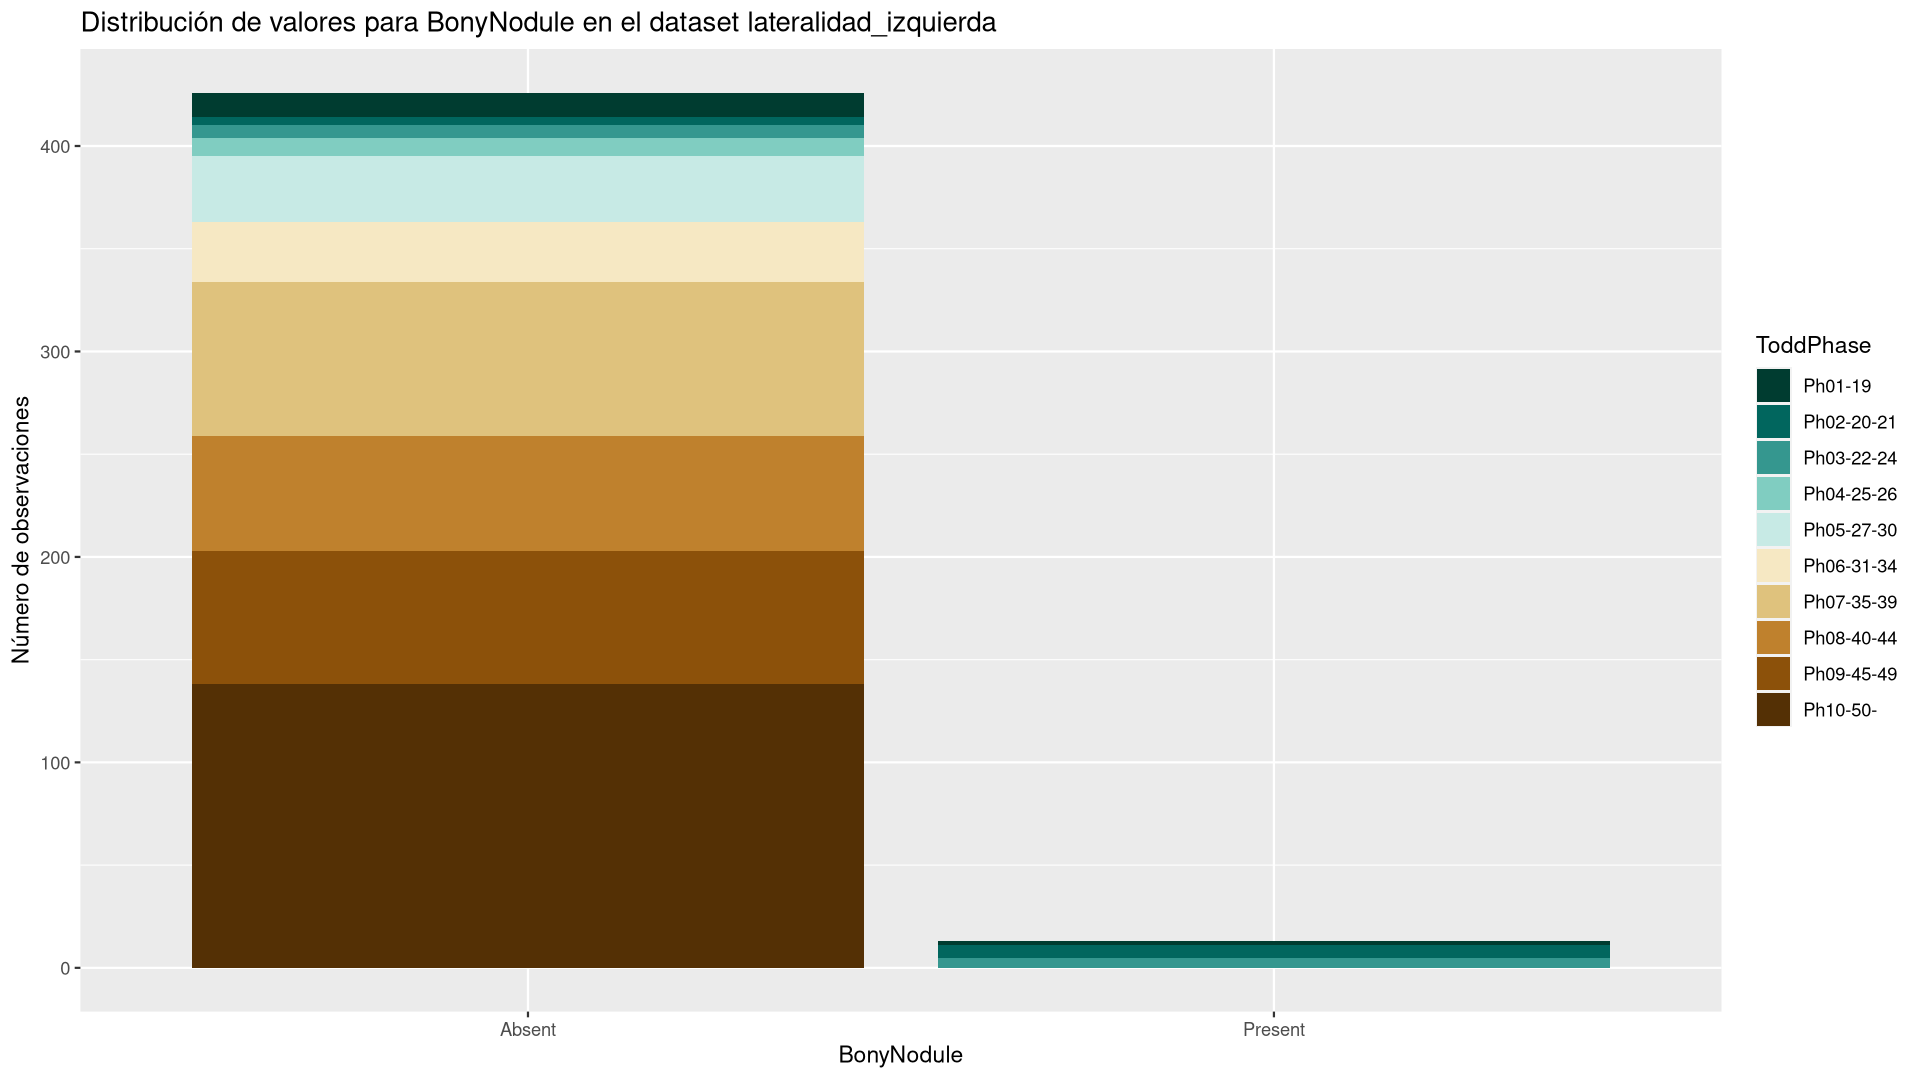
\includegraphics[width = \textwidth]{conjunto_datos/densidad_BonyNodule_lateralidad_izquierda.png}
	\caption{Distribución de los valores de BonyNodule en el conjunto de datos de la lateralidad izquierda.}
	\label{fig:densidad_BonyNodule_lateralidad_izquierda}
\end{figure}

Para la variable \texttt{BonyNodule} ocurre lo mismo que con la variable anterior, \texttt{UpperSymphysialExtremity}. Cuando se toma el valor de \texttt{Present} vemos como todas las observaciones son de fases bajas, aunque sigue existiendo ciertas dudas sobre la fase concreta. Cuando toma el valor de \texttt{Absent} no se puede sacar ninguna conclusión debido a que encontramos valores de todas las clases.

\begin{figure}[H]
	\centering
	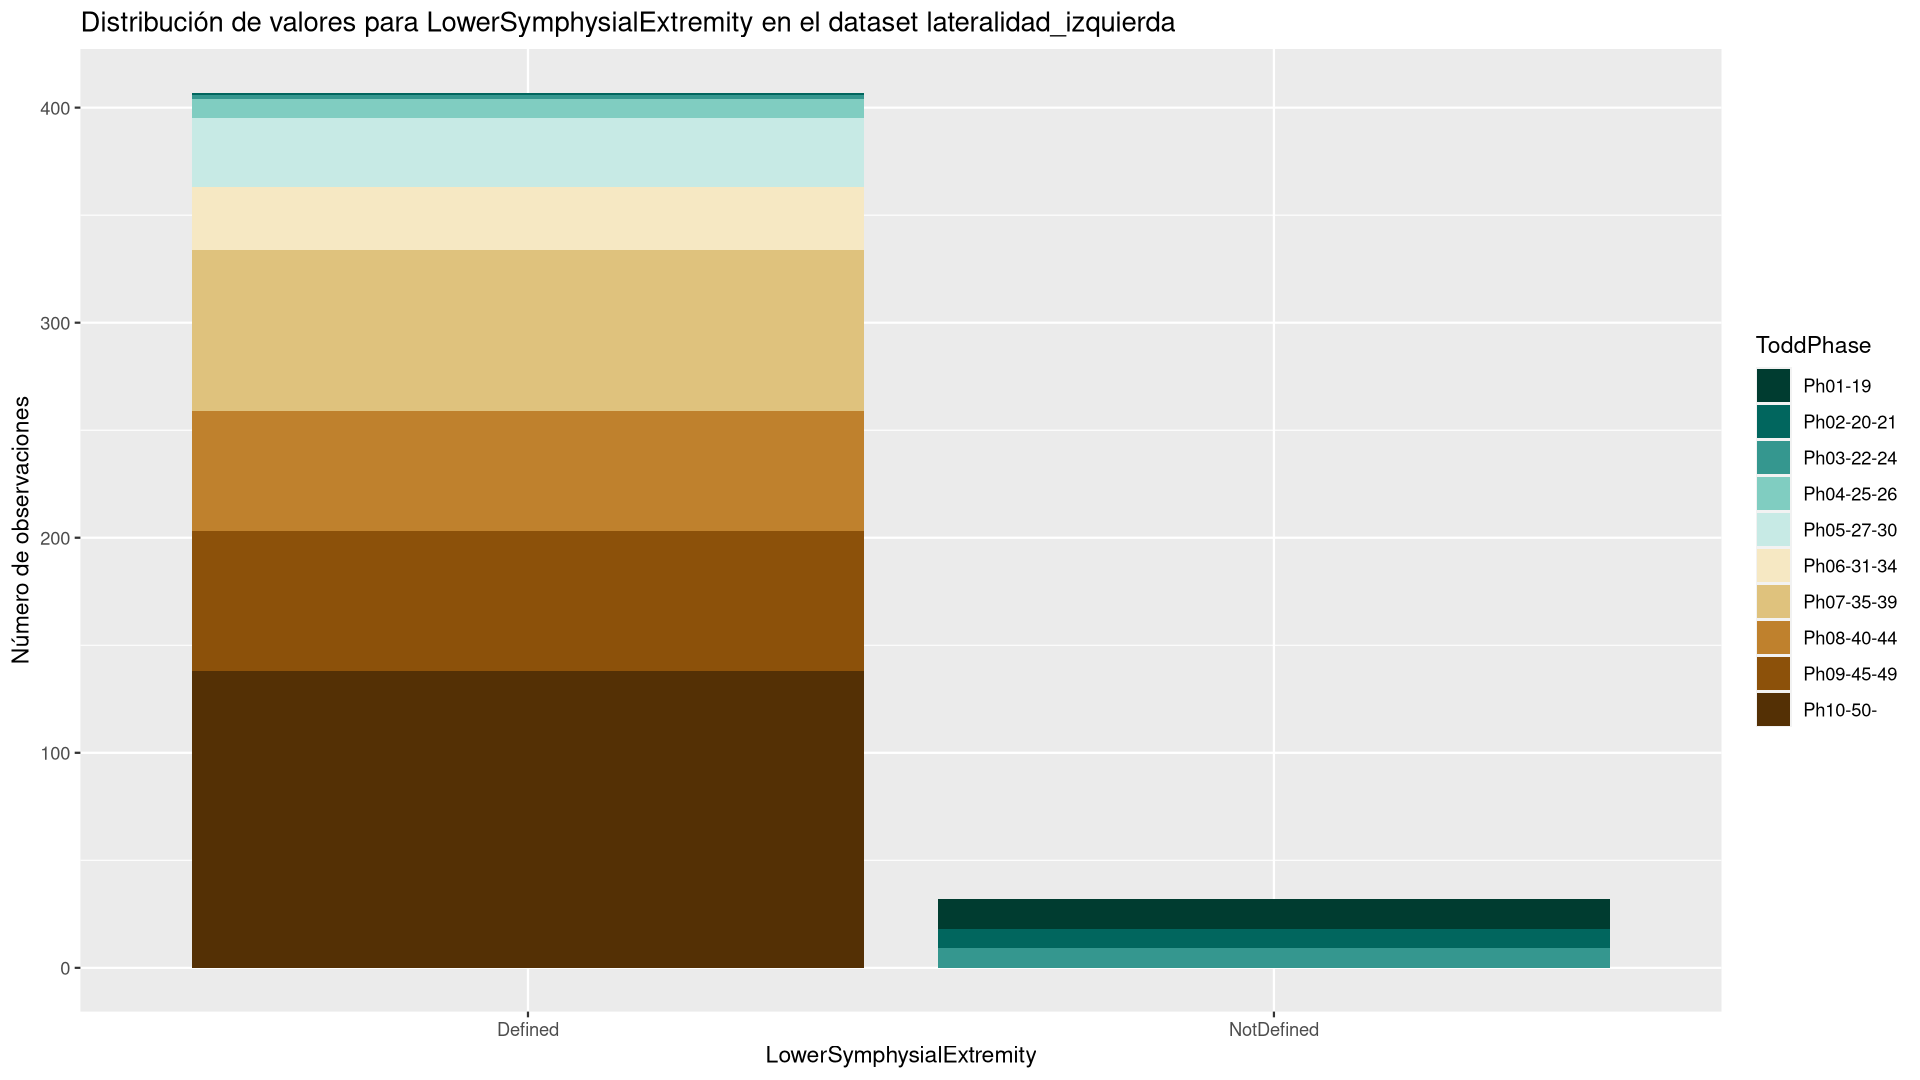
\includegraphics[width = \textwidth]{conjunto_datos/densidad_LowerSymphysialExtremity_lateralidad_izquierda.png}
	\caption{Distribución de los valores de LowerSymphysialExtremity en el conjunto de datos de la lateralidad izquierda.}
	\label{fig:densidad_LowerSymphysialExtremity_lateralidad_izquierda}
\end{figure}

Con \texttt{LowerSymphysialExtremity} se puede observar que ocurre al igual que en casos anteriores, si toma el valor \texttt{NotDefined} podemos ver que se trata de una fase baja, sin embargo, en este caso si que nos llega a aportar algo más de información. En los casos anteriores, aunque un valor nos discriminaba muy bien si era de una fase temprana o no, el valor contrario seguía teniendo valores de todas las clases, es decir, si por ejemplo \texttt{BonyNodule} toma el valor \texttt{Present}, sabemos que se trata de una fase temprana, sin embargo si toma el valor \texttt{Absent} no podemos decir nada, porque podría ser de cualquier fase, sin embargo, con \texttt{LowerSymphysialExtremity} podemos ver claramente como si es \texttt{NotDefined} será de una clase baja, pero si es \texttt{Defined} podemos concluir que, al menos de la primera fase no será esta observación, ya que no encontramos observaciones de esta fase, y muy pocas de la fase dos y tres.

\begin{figure}[H]
	\centering
	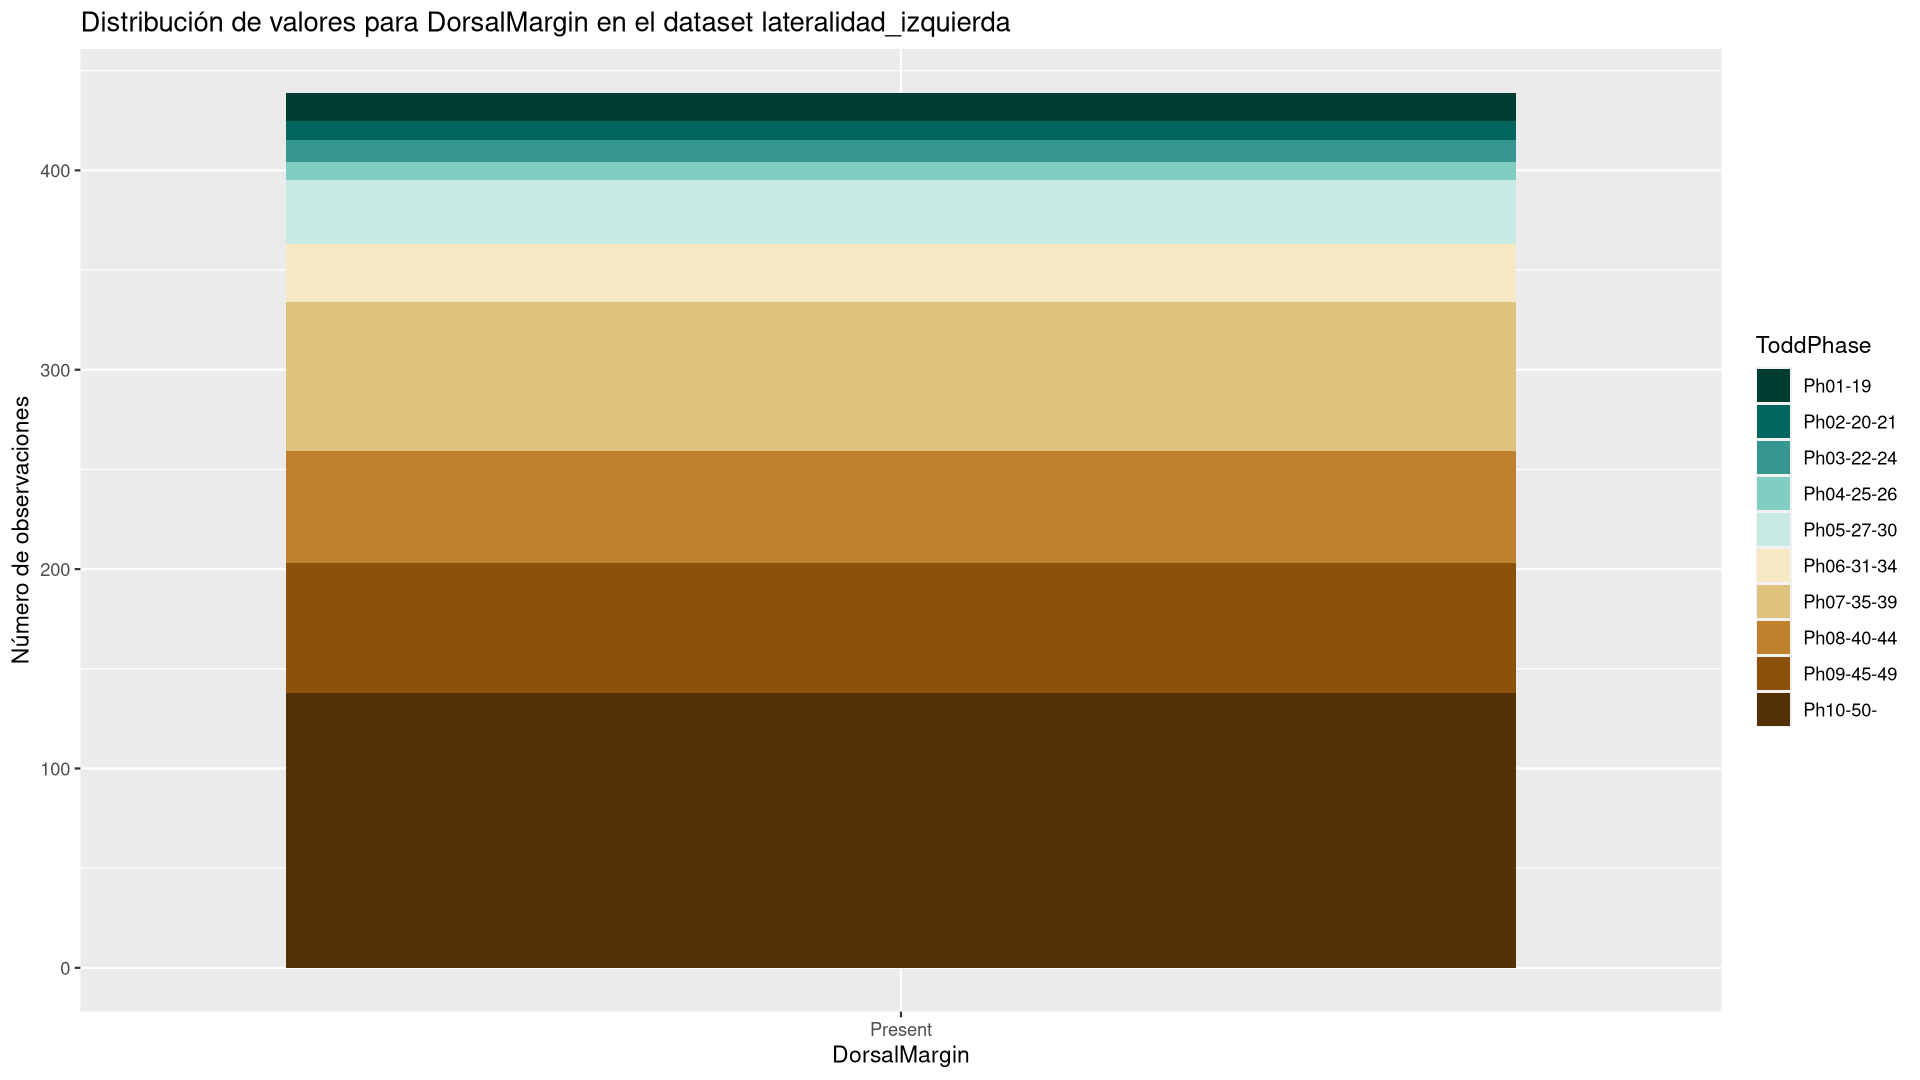
\includegraphics[width = \textwidth]{conjunto_datos/densidad_DorsalMargin_lateralidad_izquierda.png}
	\caption{Distribución de los valores de DorsalMargin en el conjunto de datos de la lateralidad izquierda.}
	\label{fig:densidad_DorsalMargin_izquierda}
\end{figure}

En este caso \texttt{DorsalMargin} vemos como no aporta información alguna, ya que solo toma un valor independientemente de la fase de edad. Si esto sigue ocurriendo en la lateralidad derecha (y por lo tanto en el conjunto completo, al ser la unión de este conjunto y la lateralidad derecha), podemos eliminar esta característica a la hora de entrenar el modelo ya que no aportaría información alguna al modelo.

\begin{figure}[H]
	\centering
	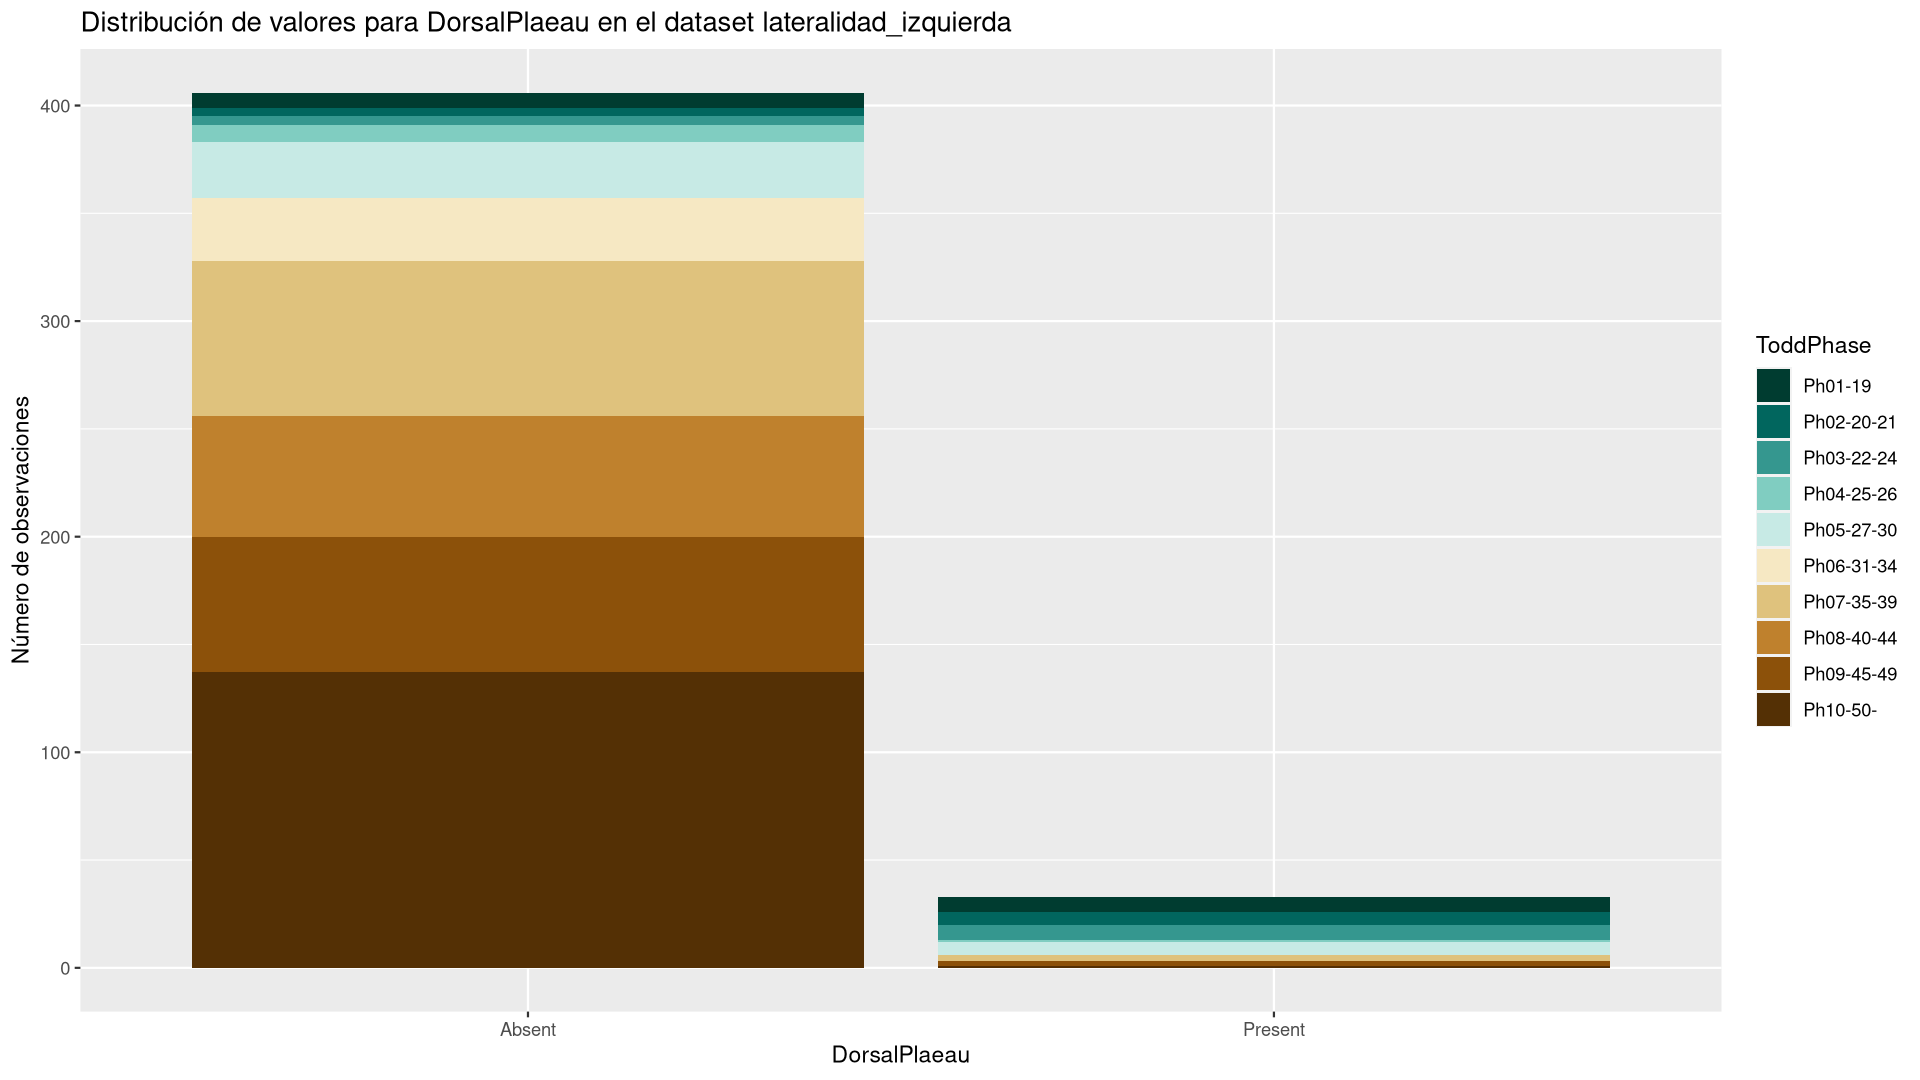
\includegraphics[width = \textwidth]{conjunto_datos/densidad_DorsalPlaeau_lateralidad_izquierda.png}
	\caption{Distribución de los valores de DorsalPlaeau en el conjunto de datos de la lateralidad izquierda.}
	\label{fig:densidad_DorsalPlaeau_izquierda}
\end{figure}

Para los valores de \texttt{DorsalPlaeau} vemos como si que toma distintos valores, sin embargo estos no nos aportan mucha información, ya que tanto para \texttt{Absent} como para \texttt{Present} contamos con observaciones de todo tipo de fases, tanto altas como bajas, luego a priori no podemos saber si este predictor será de gran utilidad.

\begin{figure}[H]
	\centering
	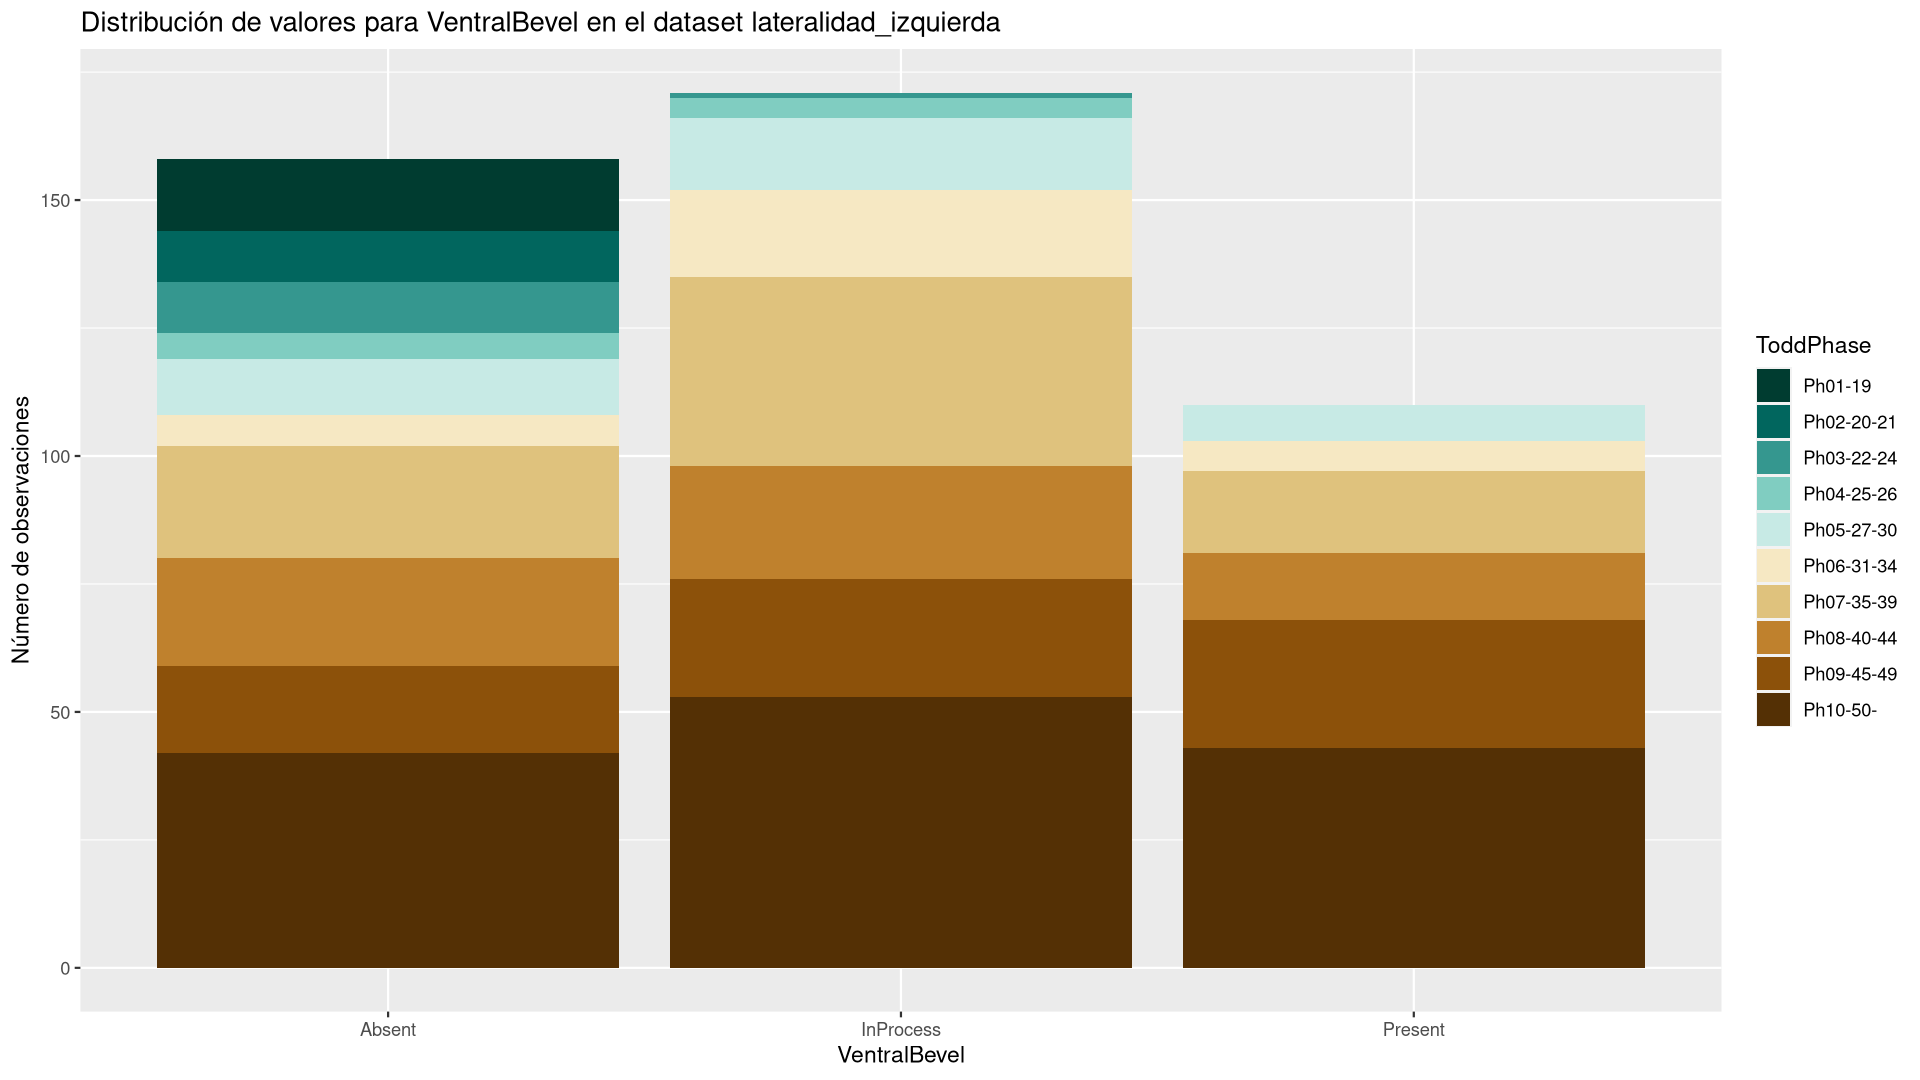
\includegraphics[width = \textwidth]{conjunto_datos/densidad_VentralBevel_lateralidad_izquierda.png}
	\caption{Distribución de los valores de VentralBevel en el conjunto de datos de la lateralidad izquierda.}
	\label{fig:densidad_VentralBevel_izquierda}
\end{figure}

Aunque con \texttt{VentralBevel} vemos como para los distintos valores tenemos una gran variedad de clases, si que podemos sacar algunas conclusiones de este gráfico, voy a comentarlas según cada valor que puede tomar esta variable. Empezando con \texttt{Absent}, podemos ver como no podemos sacar ninguna conclusión, al tener observaciones de todo tipo de fases. Con \texttt{InProcess} se observa que aunque sigue existiendo observaciones de casi todas las fases, no tenemos de la fase uno, y las observaciones de la fase dos sin mínimas. Esto sumado a que con valores de \texttt{Present} solo se tienen observaciones de fases mayores a la fase cinco, este predictor nos puede ser de utilidad para acotar el resultado, ya que gran cantidad de observaciones toman el valor de \texttt{Present}, y con esto sabemos que son de una fase más alta y aunque siga existiendo variedad de clases, hemos conseguido acotarla.


\begin{figure}[H]
	\centering
	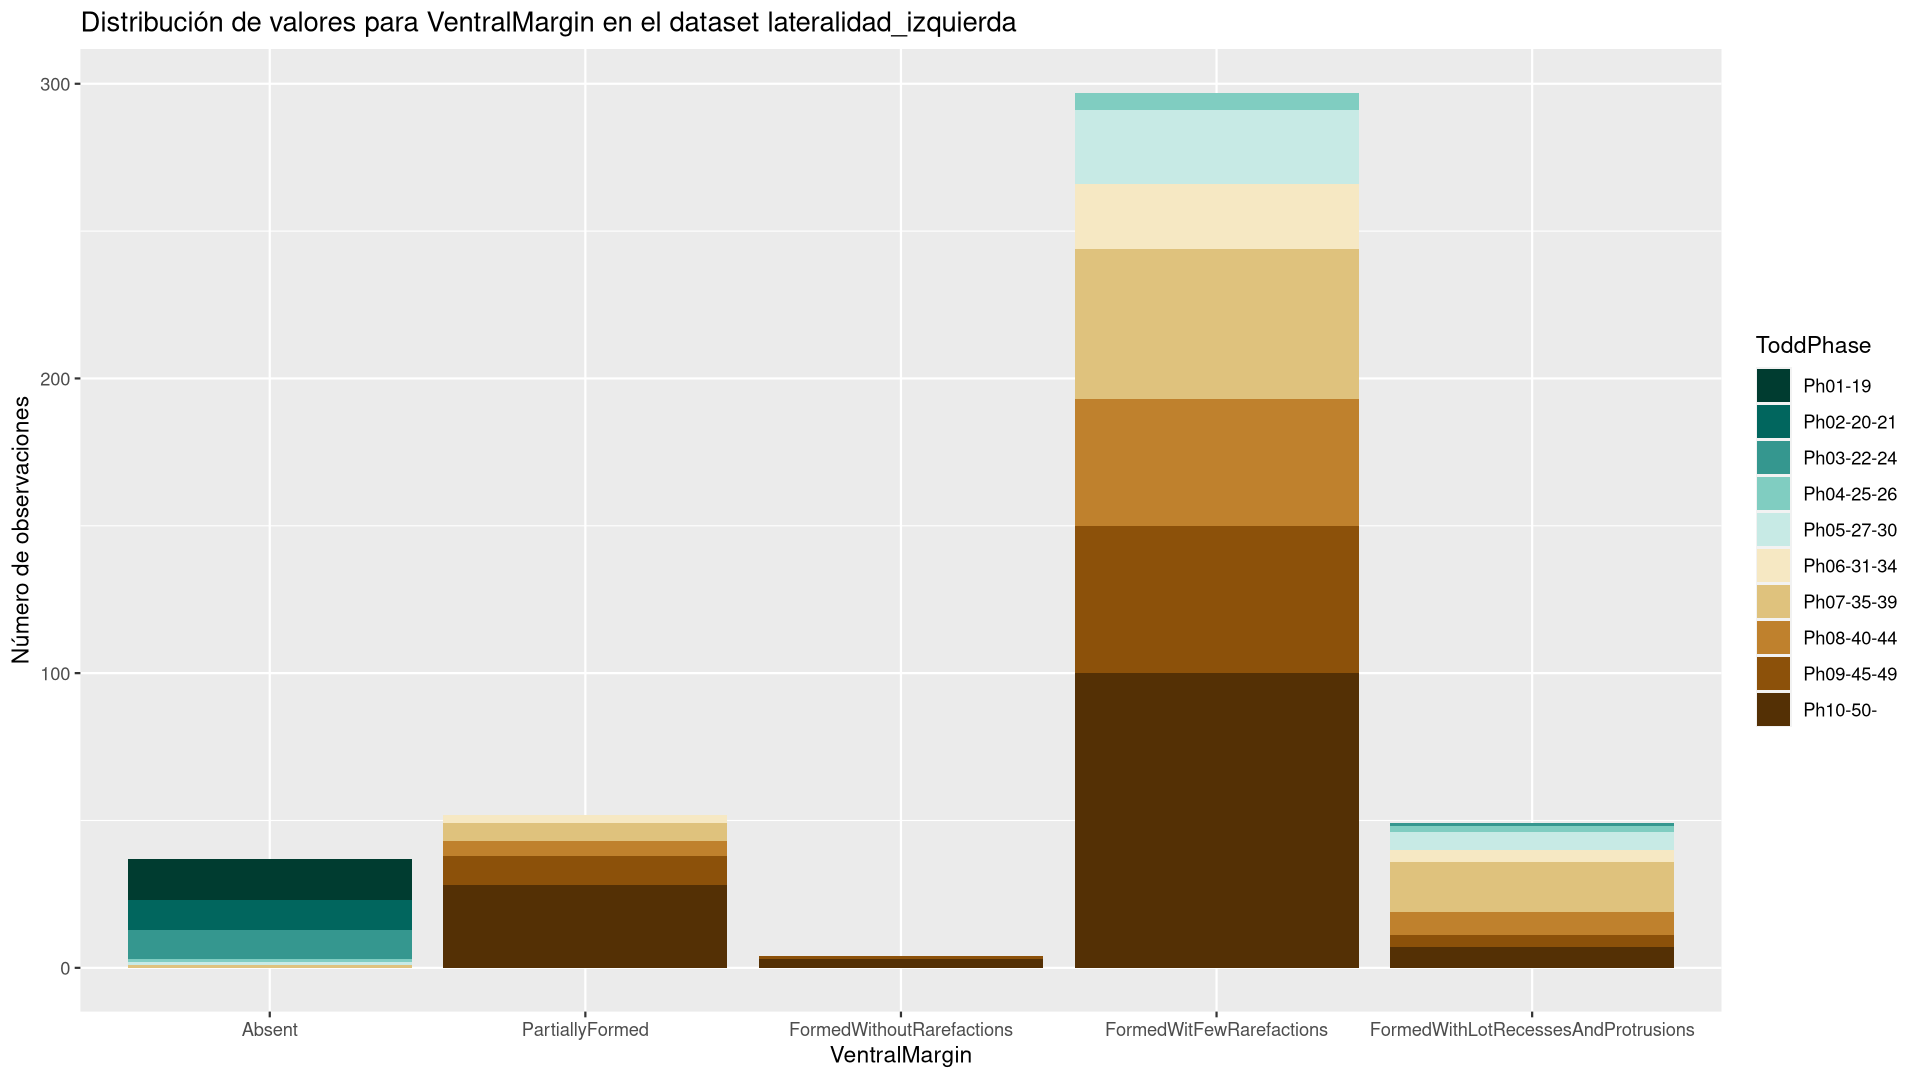
\includegraphics[width = \textwidth]{conjunto_datos/densidad_VentralMargin_lateralidad_izquierda.png}
	\caption{Distribución de los valores de VentralMargin en el conjunto de datos de la lateralidad izquierda.}
	\label{fig:densidad_VentralMargin_izquierda}
\end{figure}

Para \texttt{VentralMargin} vemos como claramente si toma el valor de \texttt{Absent} nos indica que la observación de una fase temprana, si toma el valor de \texttt{PartiallyFormed} estamos ante una observación de una fase mayor o igual a la sexta, y si toma el valor de \texttt{FormedWithoutRarefactions} se trata de una observación de la última fase. Con respecto al resto de valores, \texttt{FormedWithFewRarefactions} sigue teniendo una cantidad alta de fases, pero nos puede dar la información de que la observación no es de las tres fases más tempranas, mientras que \texttt{FormedWithLotRecessesAndProtrusions} no nos da ninguna información de la clase debido al solape de fases que existen.

\newpage

\subsubsection{Análisis de la lateralidad derecha}

Este conjunto de datos cuenta con 453 muestras. Al igual que con la lateralidad izquierda, vamos a ver de forma gráfica como se distribuyen los datos según las fases propuestas por Todd. Debido a la similitud de con la lateralidad izquierda, si las conclusiones obtenidas son semejantes a las obtenidas anteriormente para cada predictor no se comentarán por evitar repetirse:

\begin{figure}[H]
	\centering
	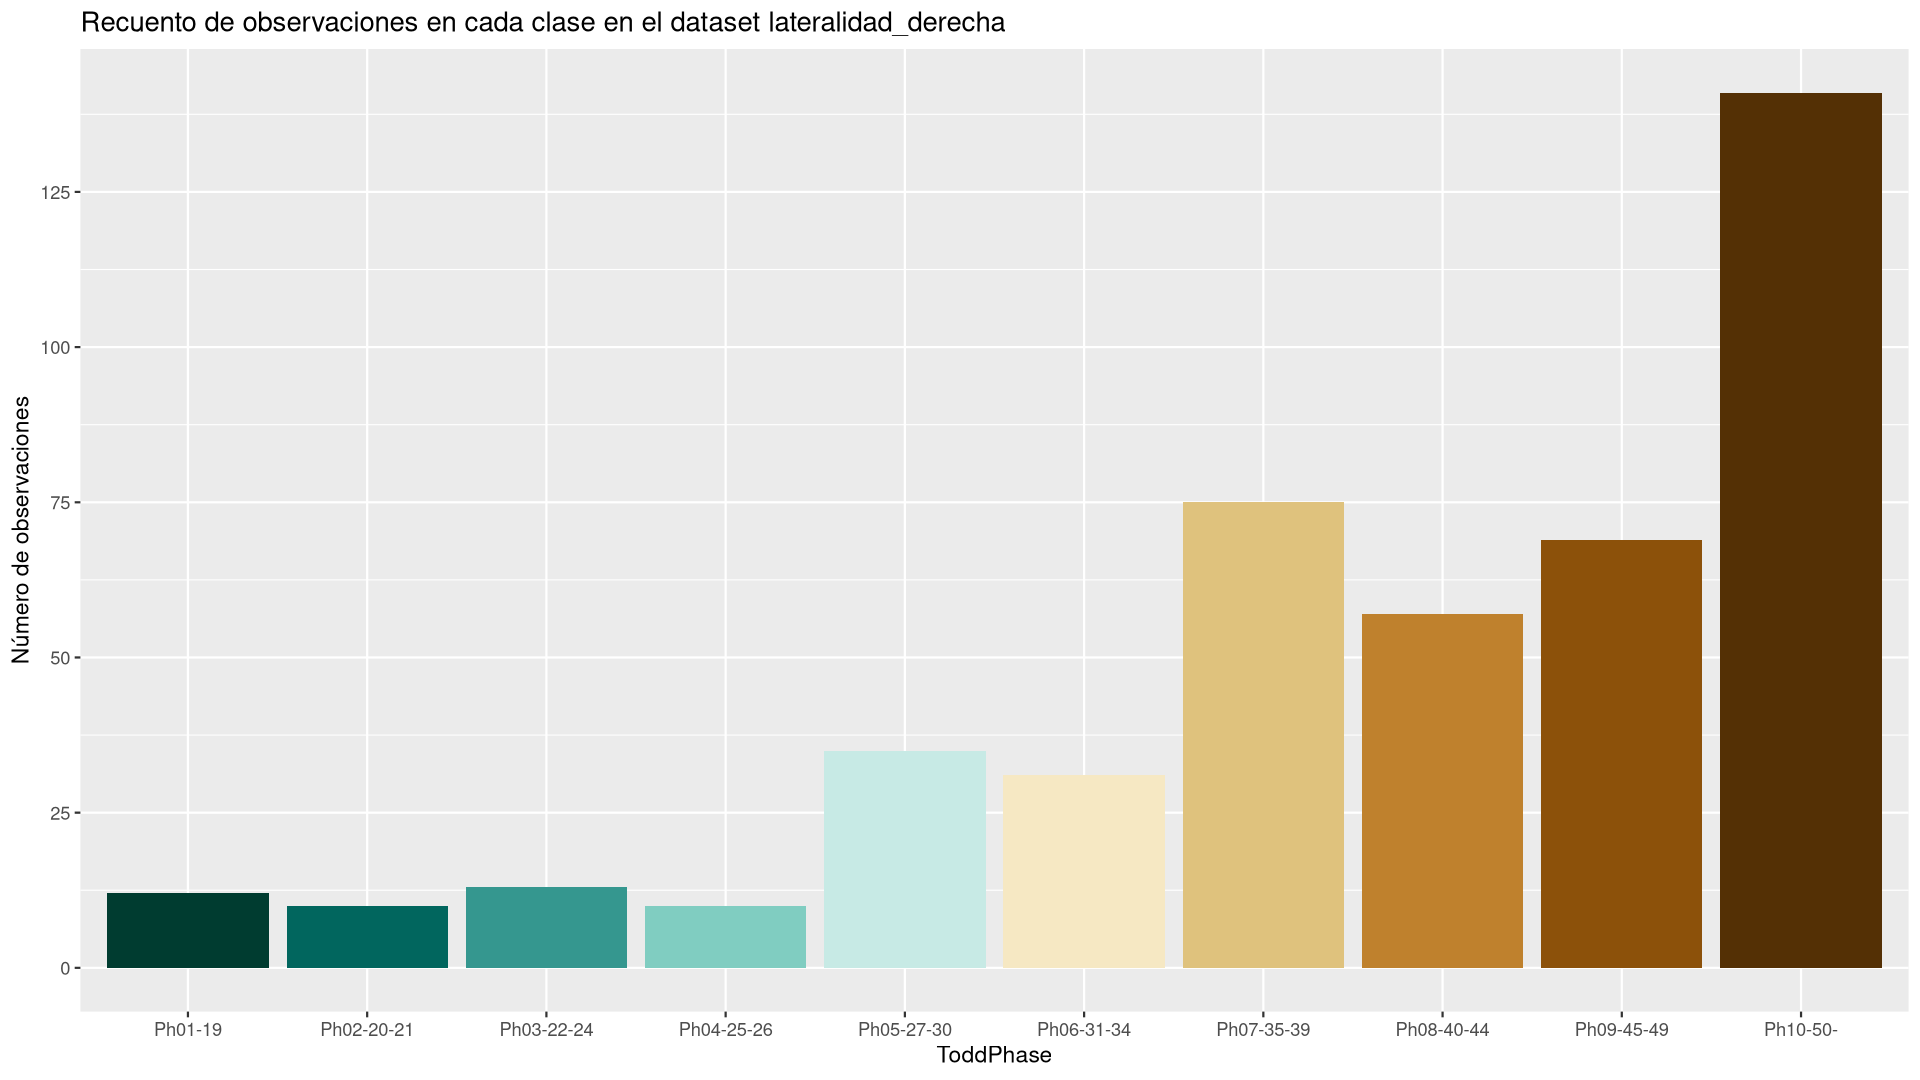
\includegraphics[width = \textwidth]{conjunto_datos/distribucion_clases_lateralidad_derecha.png}
	\caption{Número de datos por cada fase propuesta por Todd con el conjunto de datos de la lateralidad derecha.}
	\label{fig:conteo_l1}
\end{figure}


\begin{figure}[H]
	\centering
	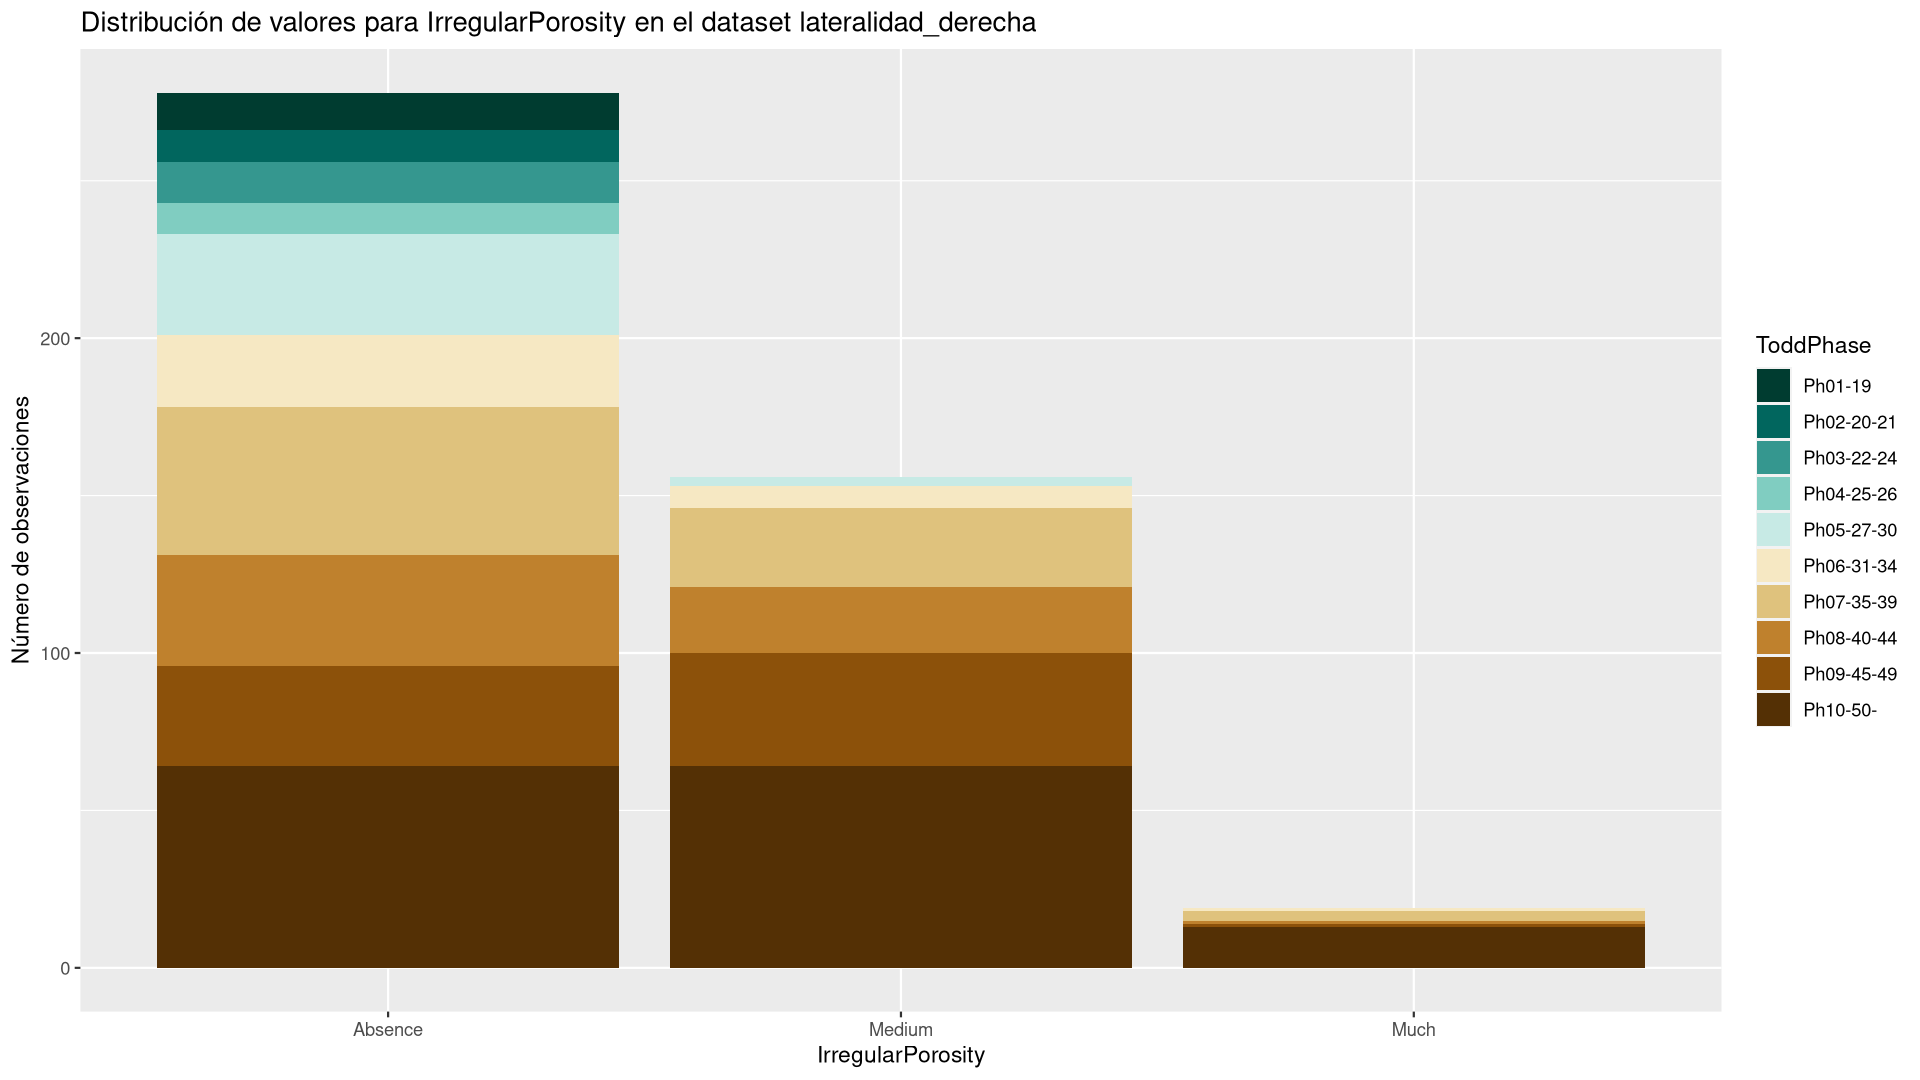
\includegraphics[width = \textwidth]{conjunto_datos/densidad_IrregularPorosity_lateralidad_derecha.png}
	\caption{Distribución de los valores de IrregularPorosity en el conjunto de datos de la lateralidad derecha.}
	\label{fig:densidad_IrregularPorosity_lateralidad_derecha}
\end{figure}

\begin{figure}[H]
	\centering
	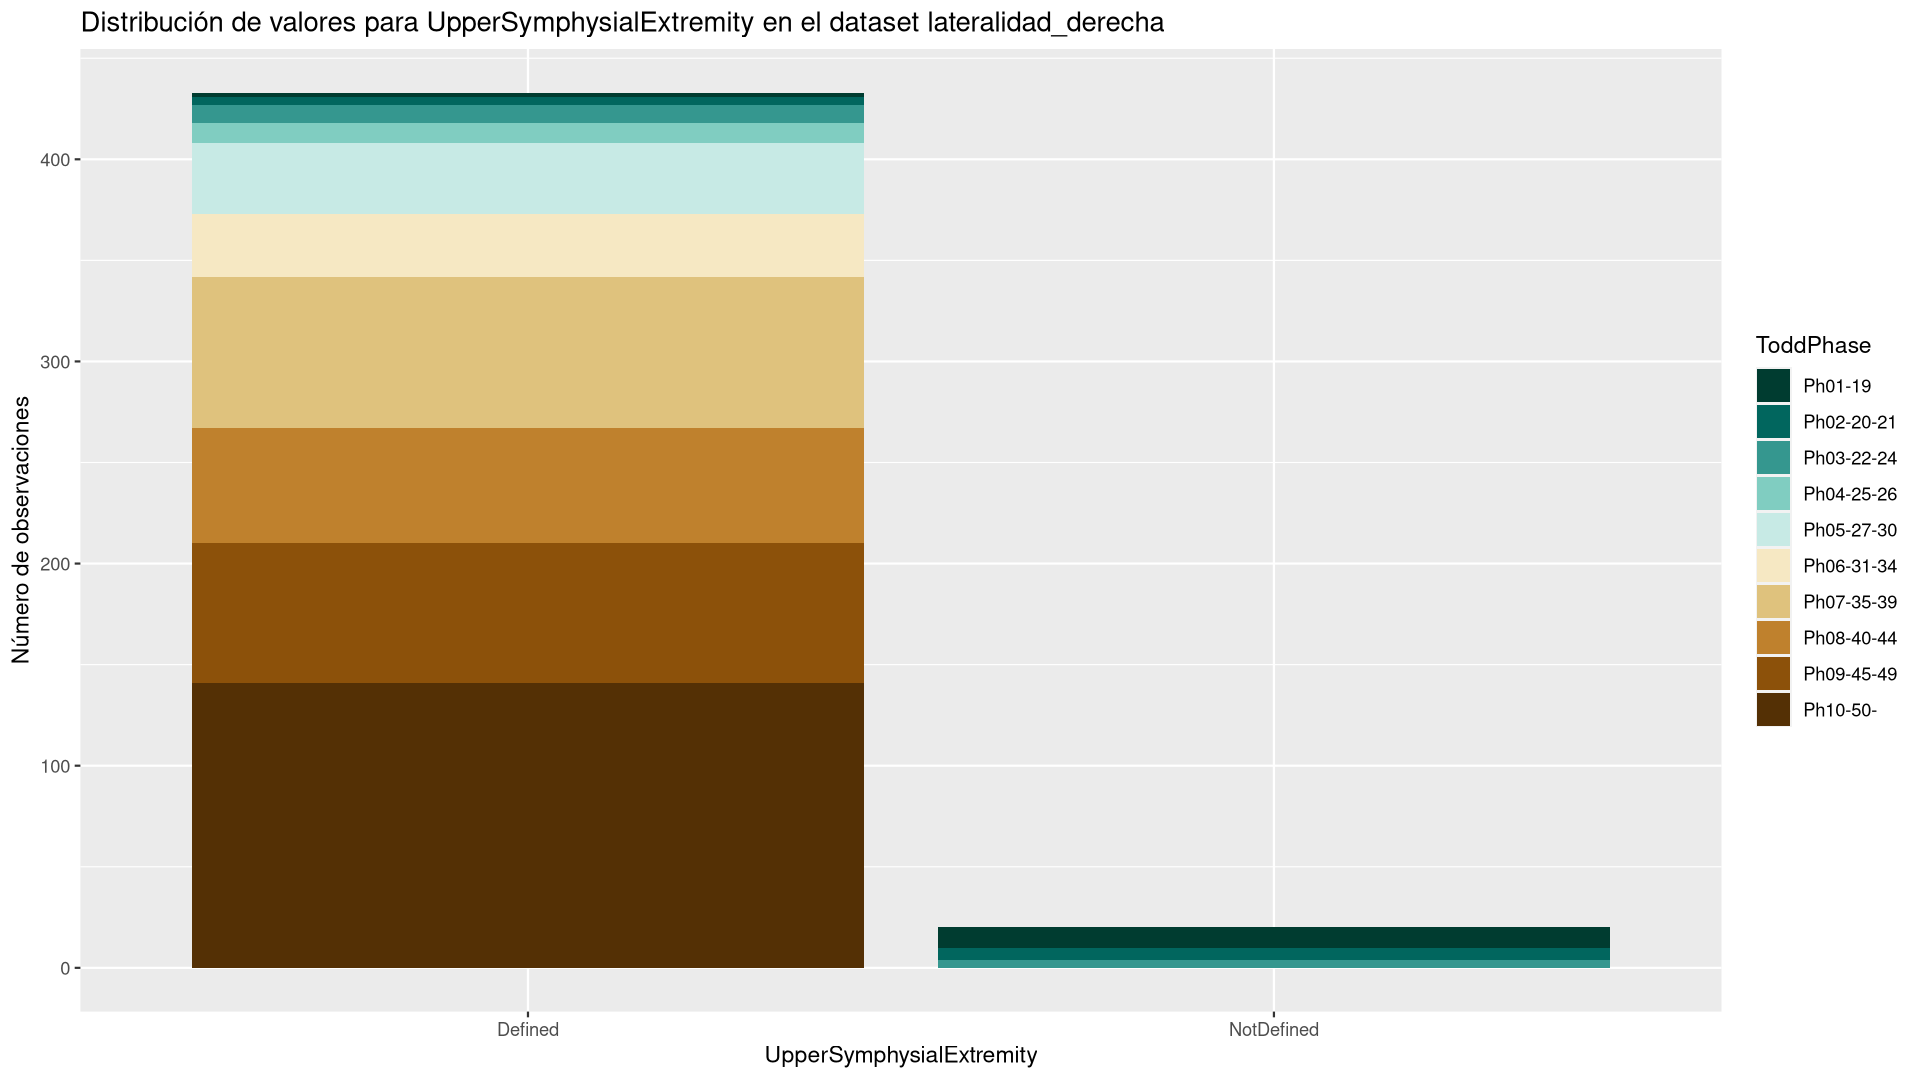
\includegraphics[width = \textwidth]{conjunto_datos/densidad_UpperSymphysialExtremity_lateralidad_derecha.png}
	\caption{Distribución de los valores de UpperSymphysialExtremity en el conjunto de datos de la lateralidad derecha.}
	\label{fig:densidad_UpperSymphysialExtremity_lateralidad_derecha}
\end{figure}


\begin{figure}[H]
	\centering
	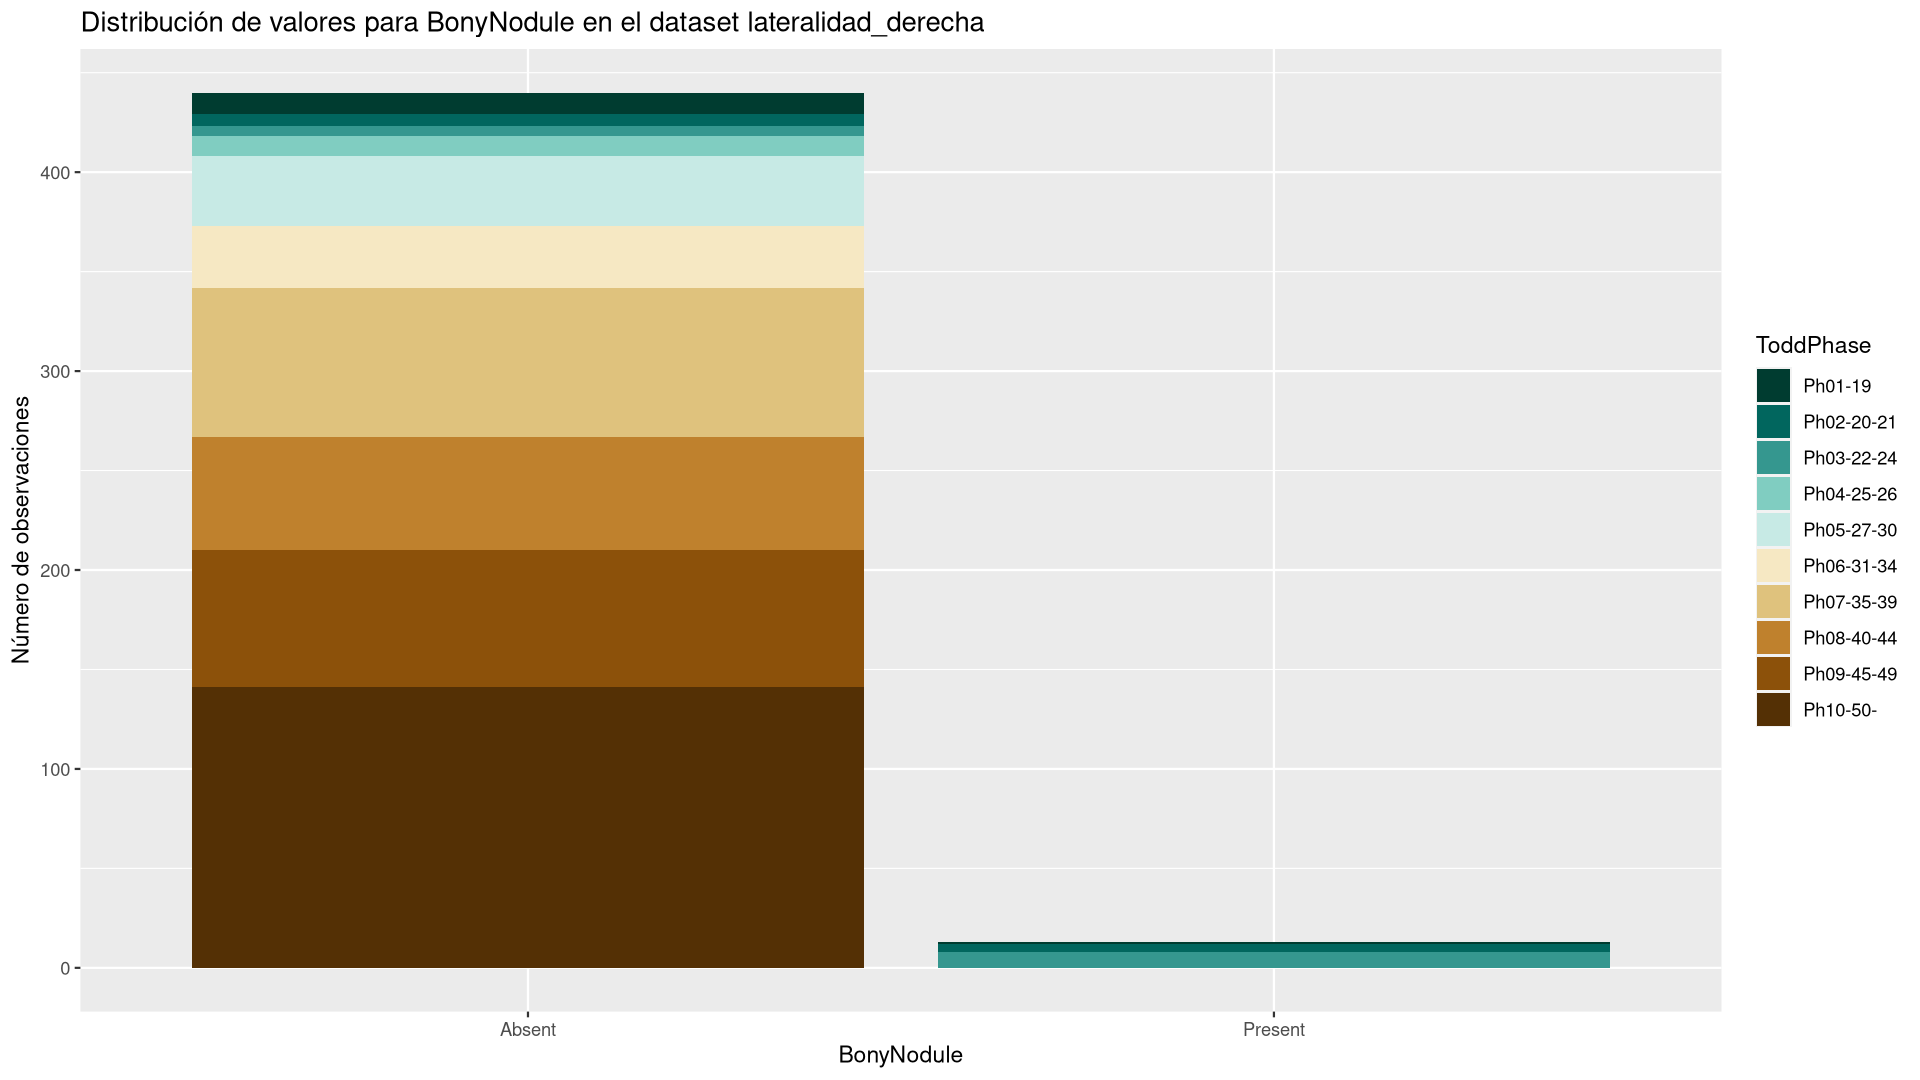
\includegraphics[width = \textwidth]{conjunto_datos/densidad_BonyNodule_lateralidad_derecha.png}
	\caption{Distribución de los valores de BonyNodule en el conjunto de datos de la lateralidad derecha.}
	\label{fig:densidad_BonyNodule_lateralidad_derecha}
\end{figure}



\begin{figure}[H]
	\centering
	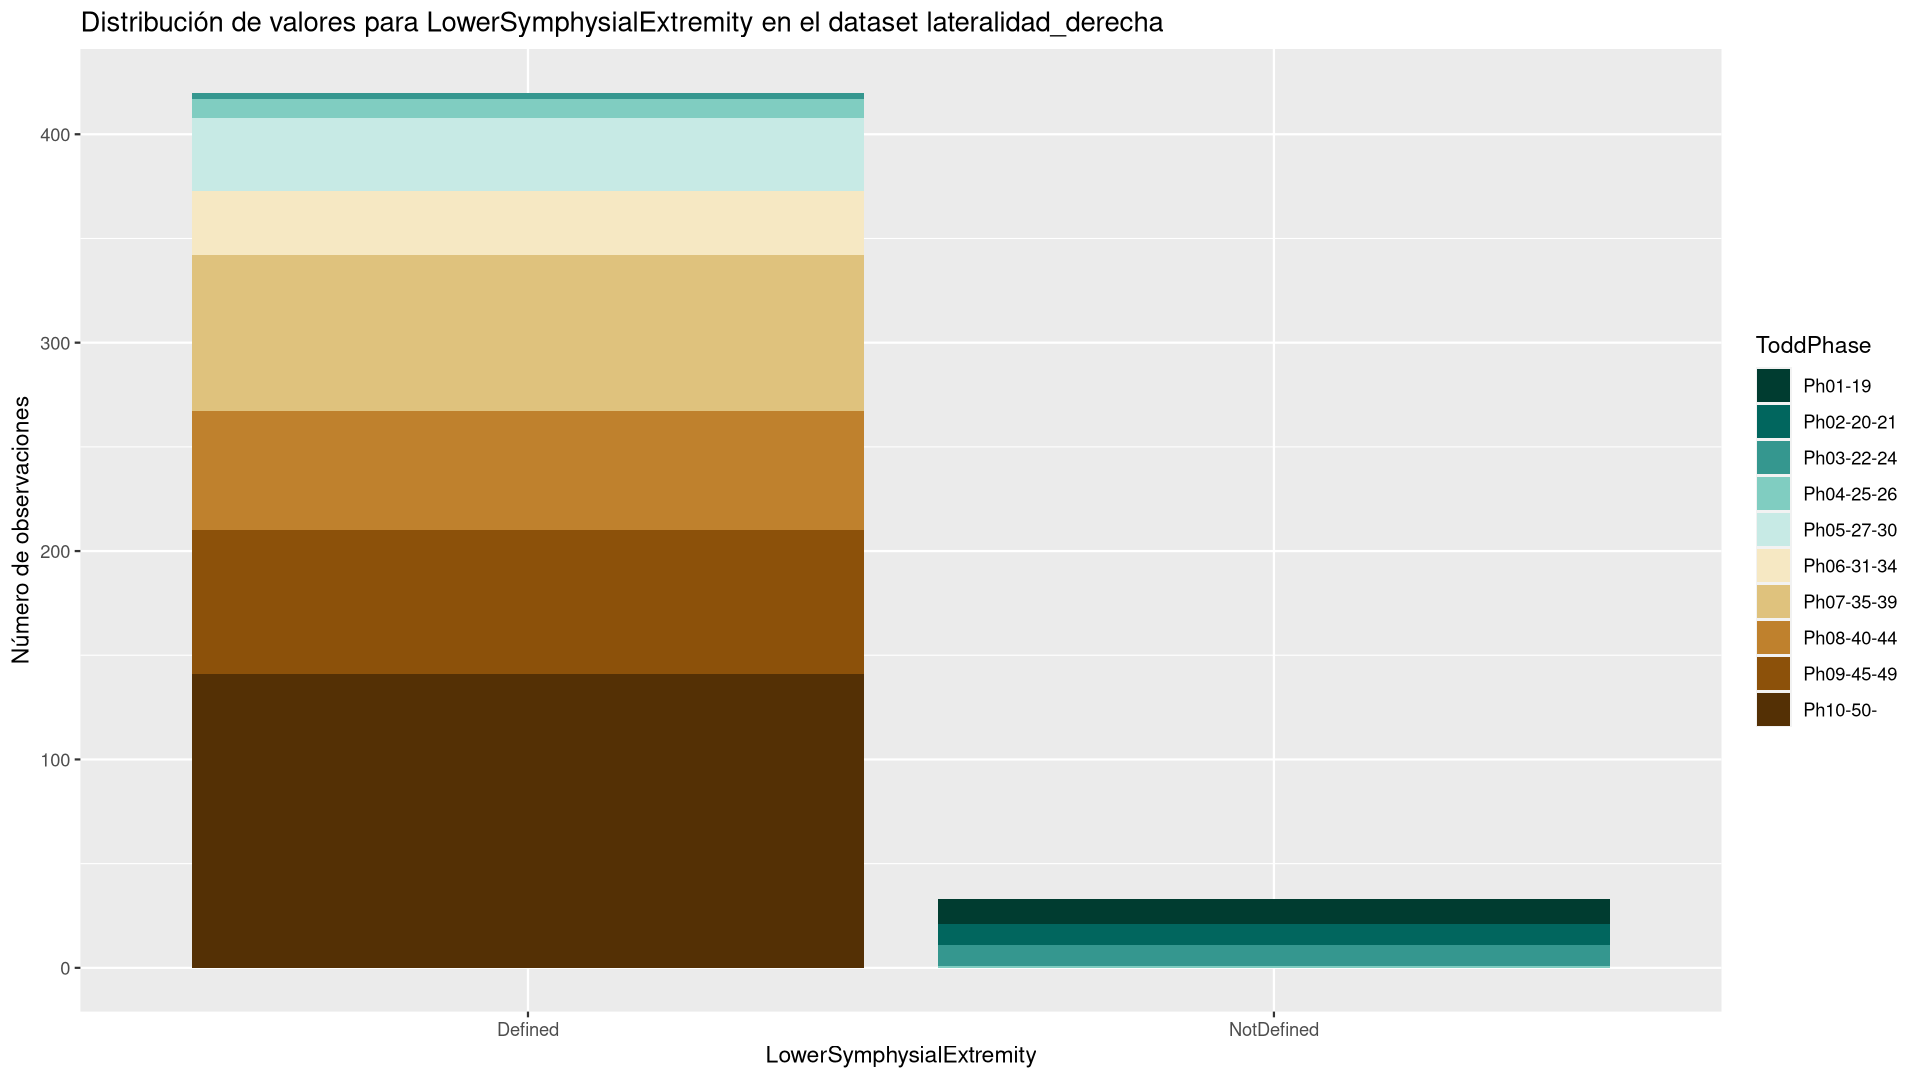
\includegraphics[width = \textwidth]{conjunto_datos/densidad_LowerSymphysialExtremity_lateralidad_derecha.png}
	\caption{Distribución de los valores de LowerSymphysialExtremity en el conjunto de datos de la lateralidad derecha.}
	\label{fig:densidad_LowerSymphysialExtremity_derecha}
\end{figure}


\begin{figure}[H]
	\centering
	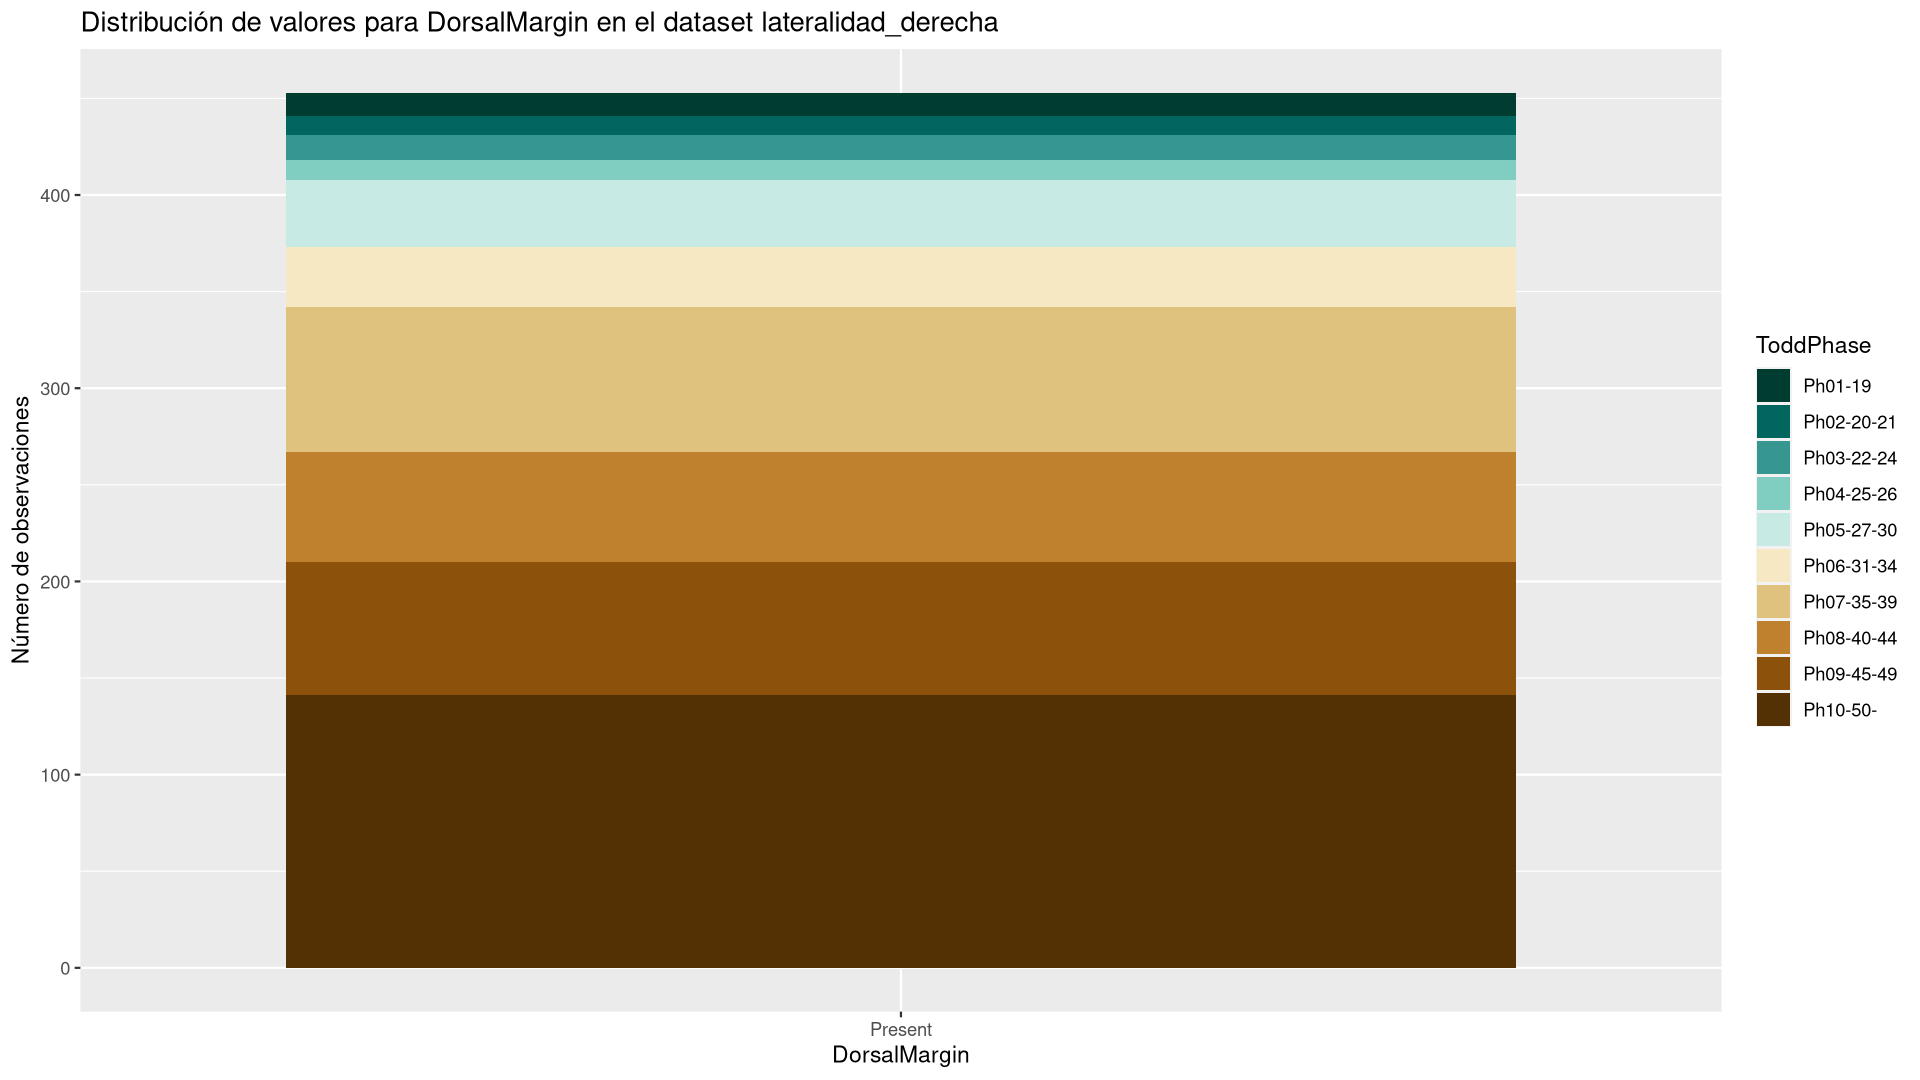
\includegraphics[width = \textwidth]{conjunto_datos/densidad_DorsalMargin_lateralidad_derecha.png}
	\caption{Distribución de los valores de DorsalMargin en el conjunto de datos de la lateralidad derecha.}
	\label{fig:densidad_DorsalMargin_derecha}
\end{figure}

\begin{figure}[H]
	\centering
	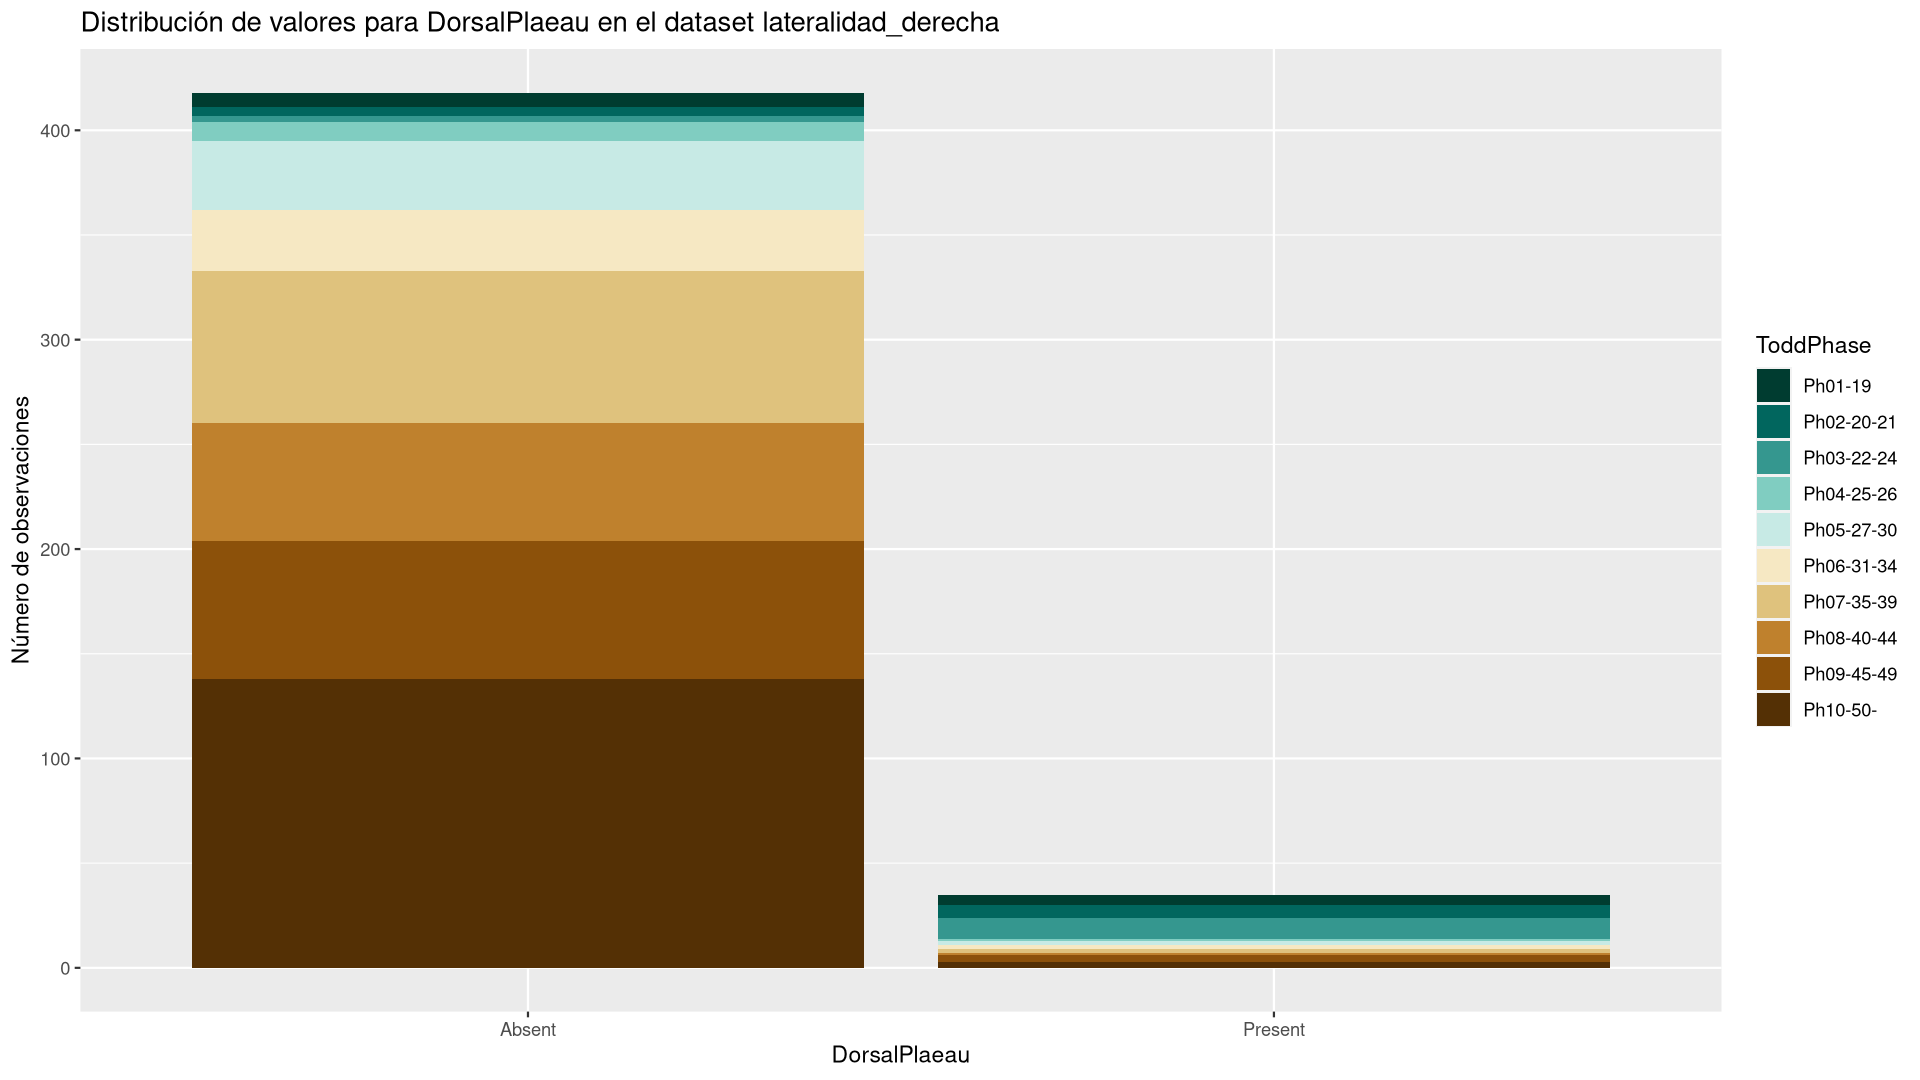
\includegraphics[width = \textwidth]{conjunto_datos/densidad_DorsalPlaeau_lateralidad_derecha.png}
	\caption{Distribución de los valores de DorsalPlaeau en el conjunto de datos de la lateralidad derecha.}
	\label{fig:densidad_DorsalPlaeau_derecha}
\end{figure}


\begin{figure}[H]
	\centering
	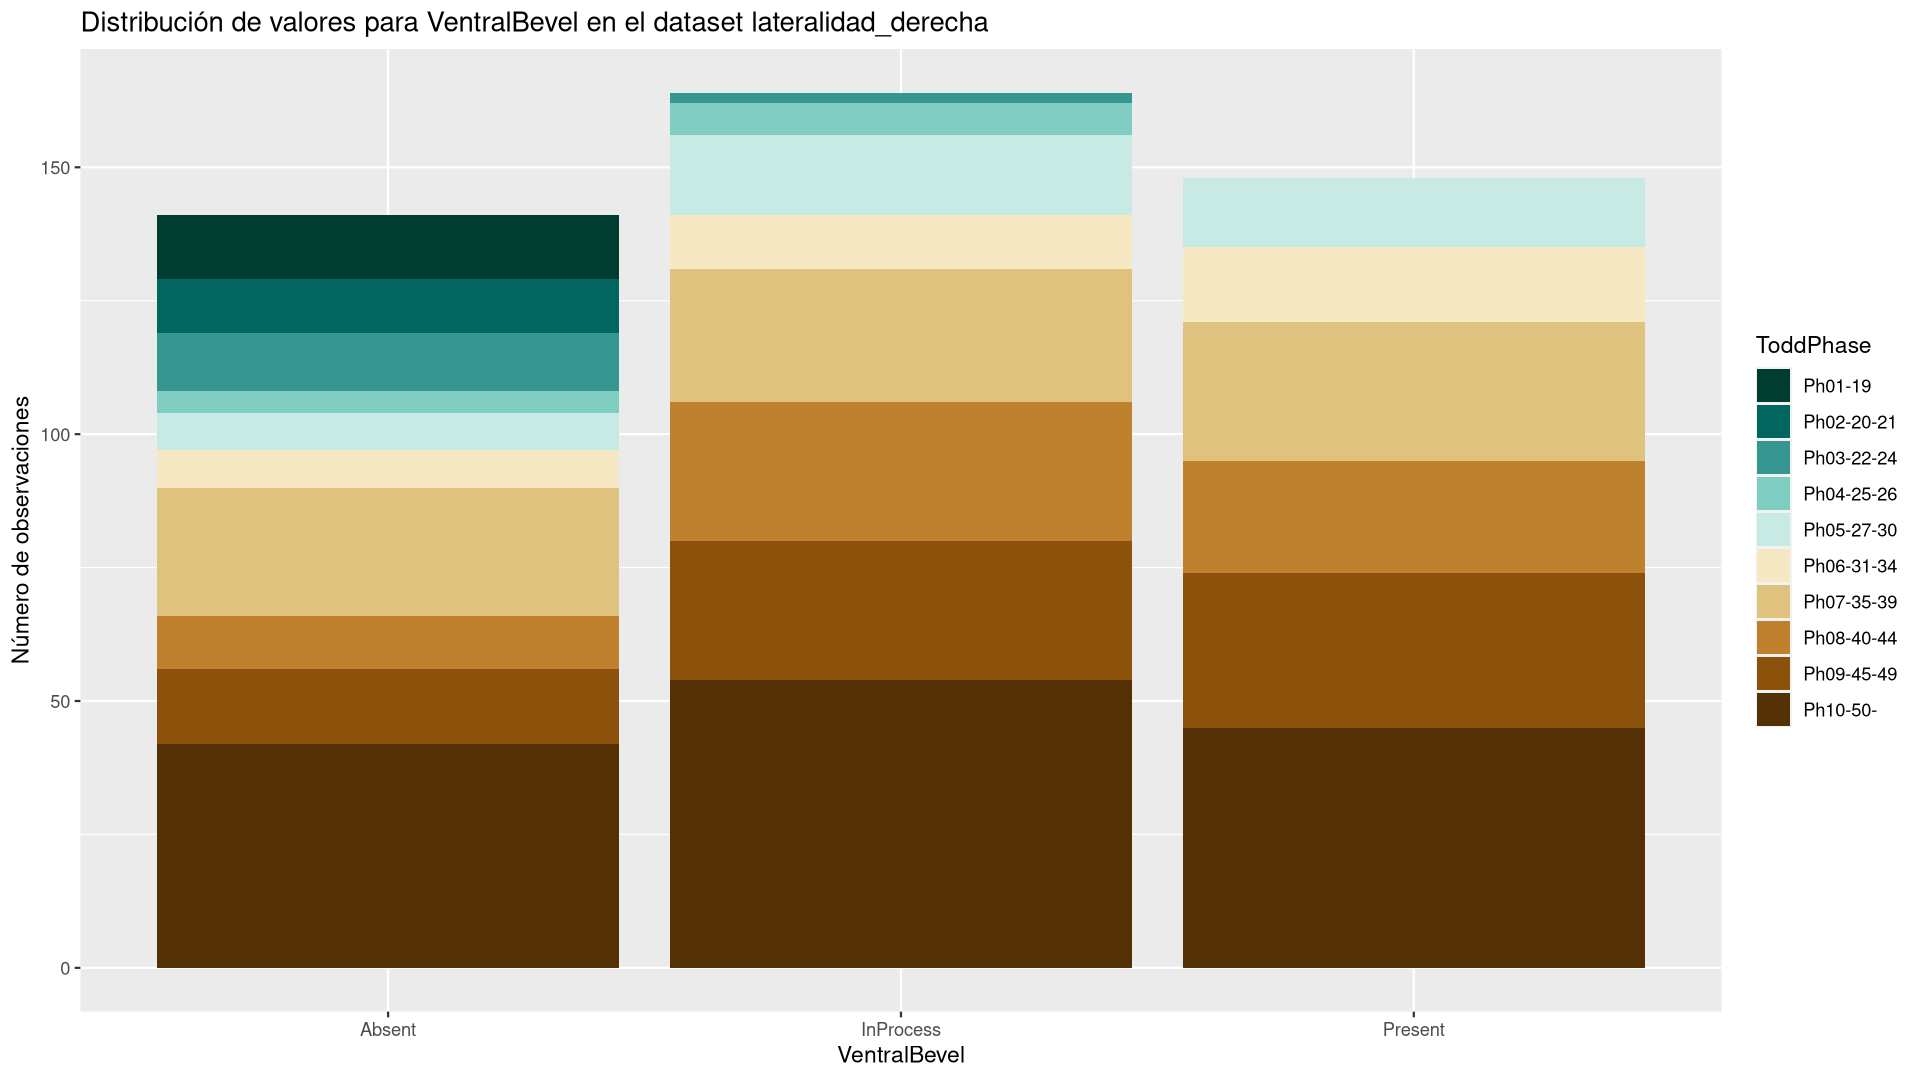
\includegraphics[width = \textwidth]{conjunto_datos/densidad_VentralBevel_lateralidad_derecha.png}
	\caption{Distribución de los valores de VentralBevel en el conjunto de datos de la lateralidad derecha.}
	\label{fig:densidad_VentralBevel_derecha}
\end{figure}

\begin{figure}[H]
	\centering
	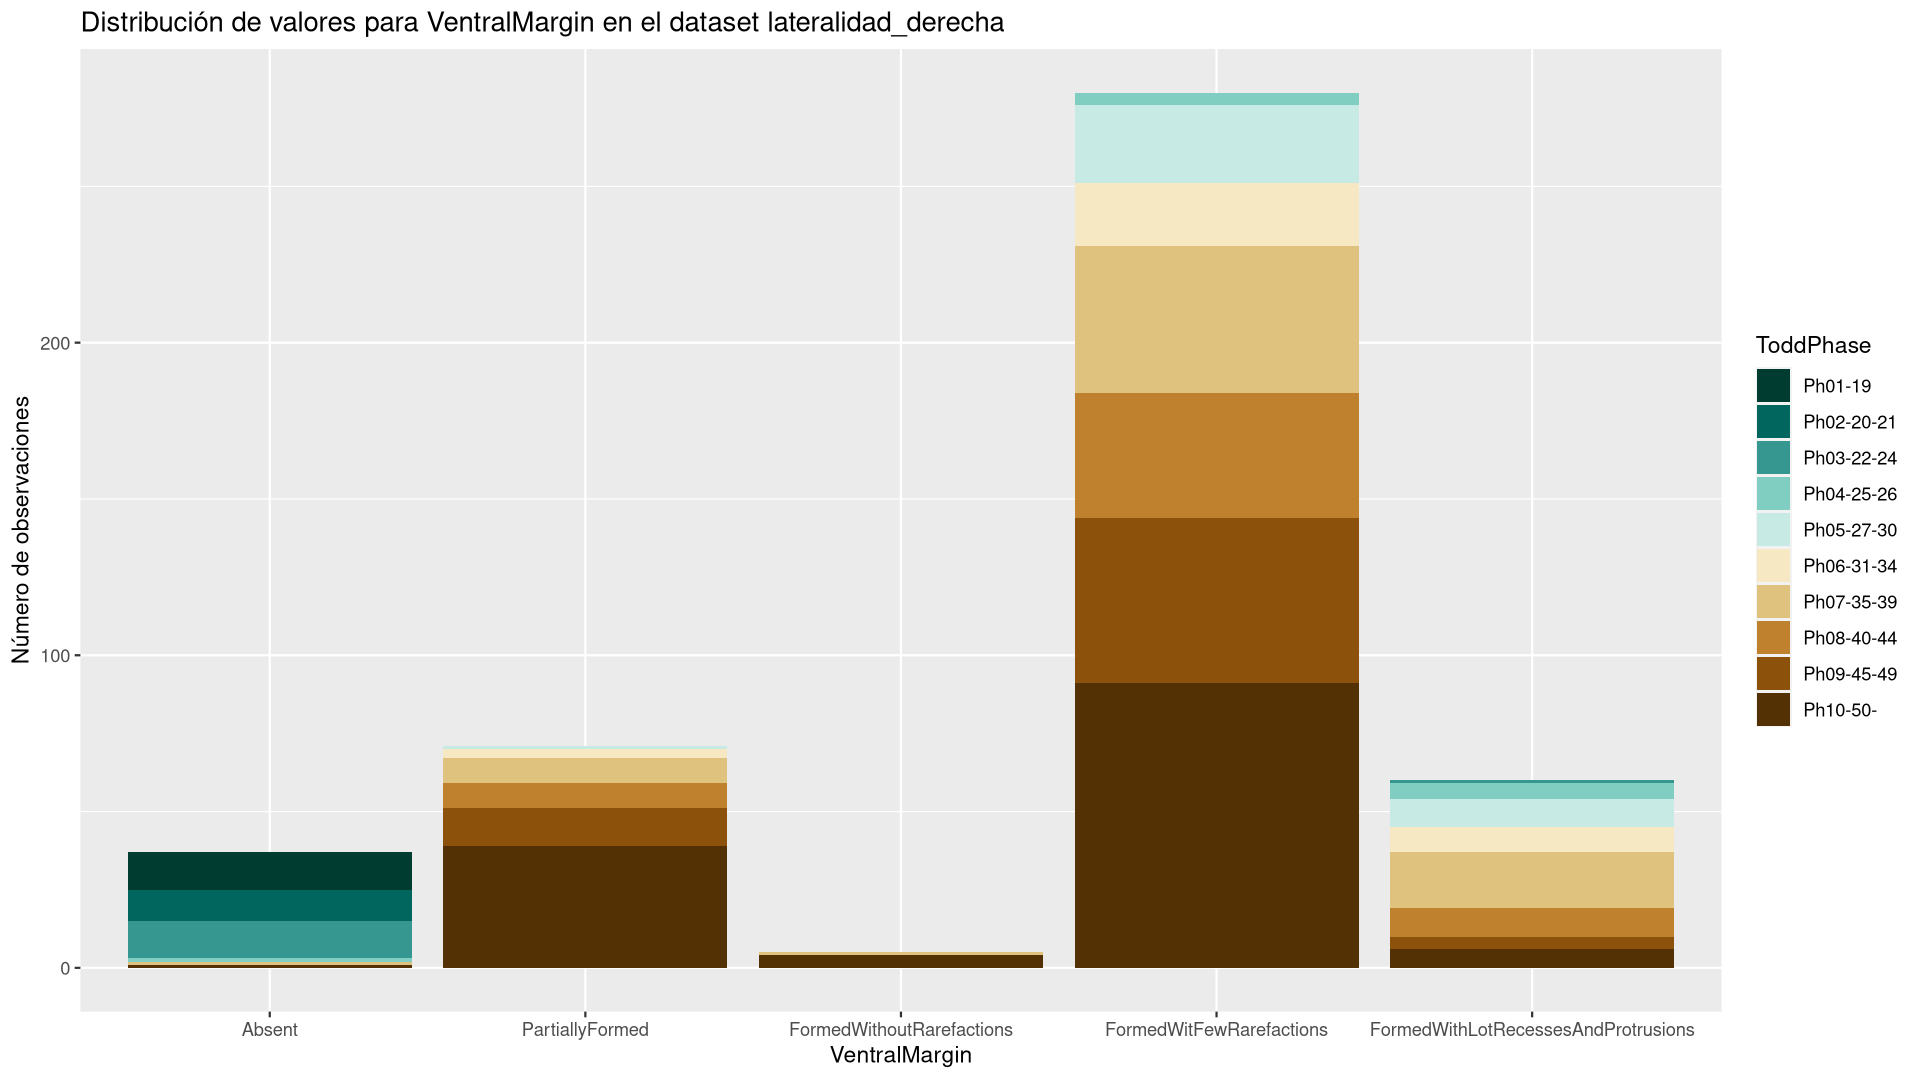
\includegraphics[width = \textwidth]{conjunto_datos/densidad_VentralMargin_lateralidad_derecha.png}
	\caption{Distribución de los valores de VentralMargin en el conjunto de datos de la lateralidad derecha.}
	\label{fig:densidad_VentralMargin_derecha}
\end{figure}

\subsubsection{Análisis del conjunto completo}

El conjunto completo de los datos cuenta con 892 observaciones, las de la lateralidad izquierda y derecha unidas. Por este motivo, al obtener las mismas conclusiones de la lateralidad izquierda y la lateralidad derecha, las conclusiones en el conjunto de datos completo cabe esperar que sean las mismas. Por este motivo simplemente vamos a comentar las más destacadas.

\begin{figure}[H]
	\centering
	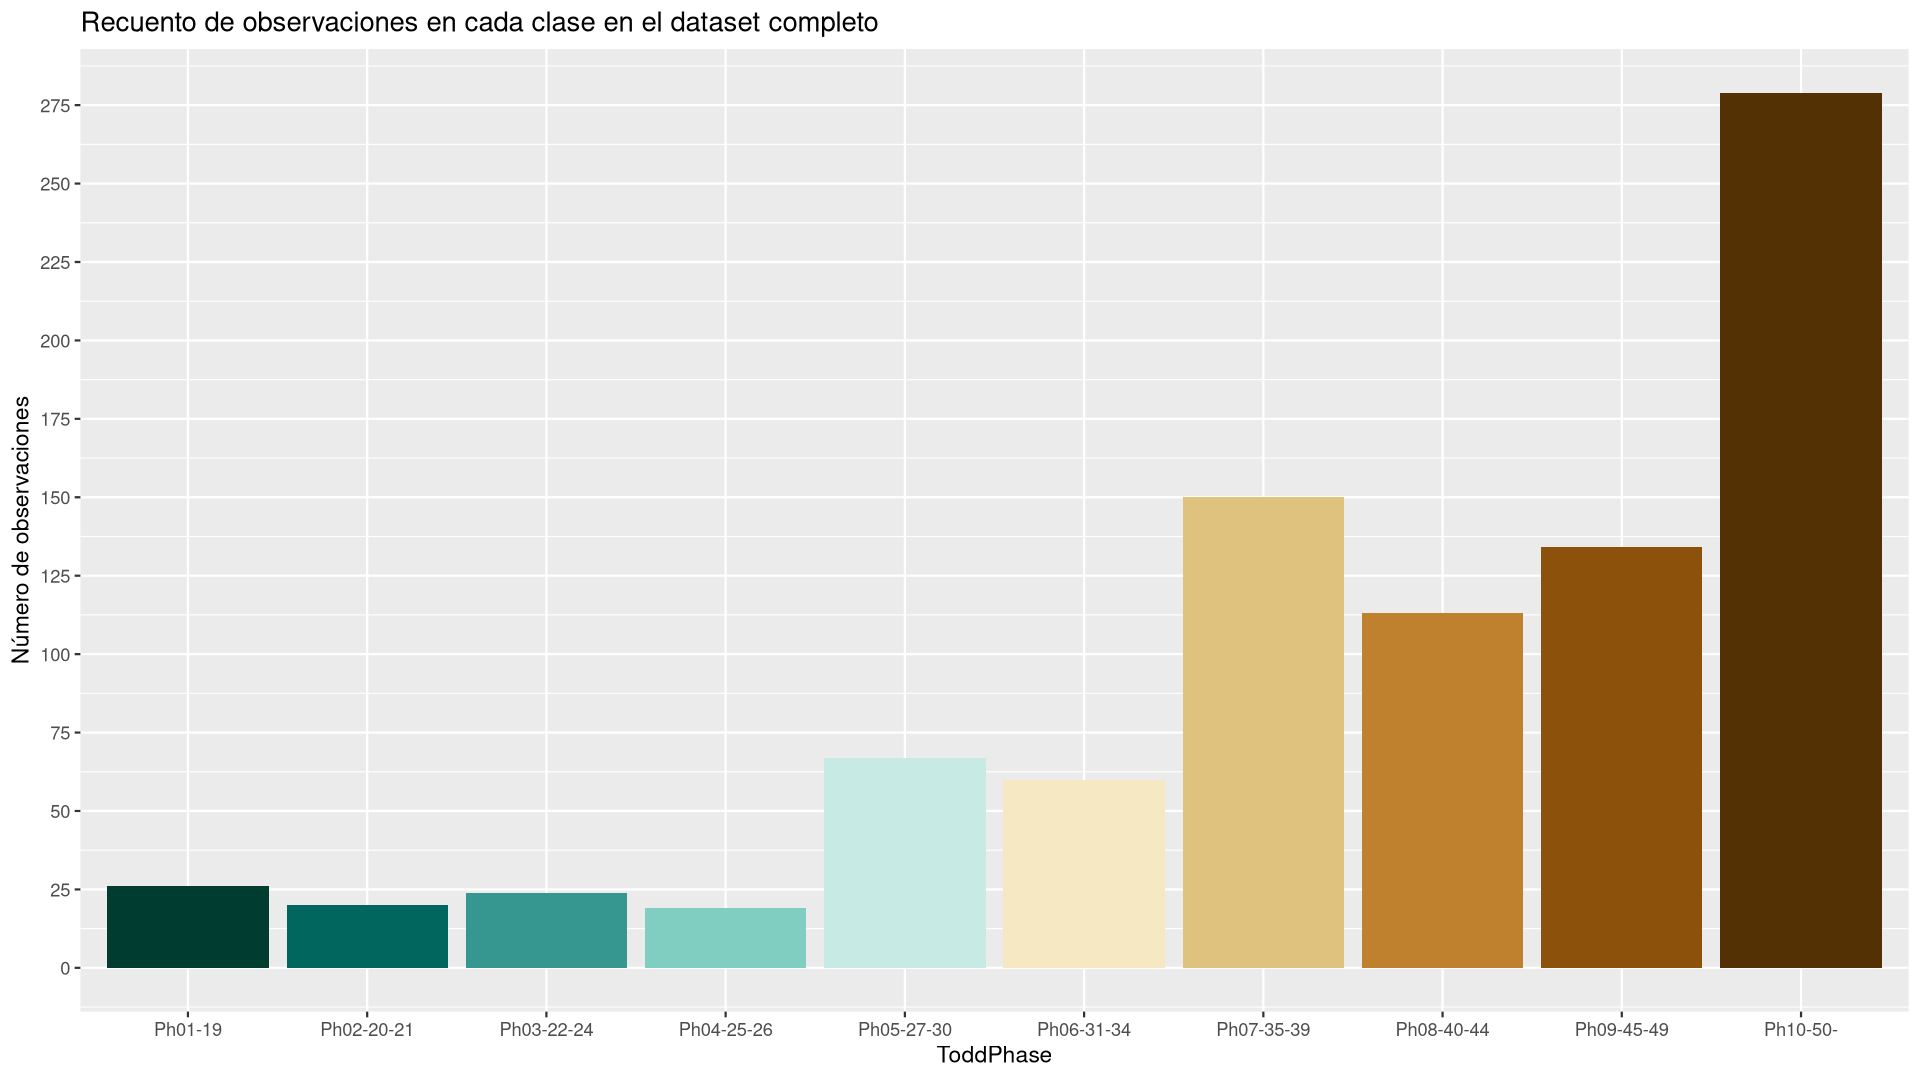
\includegraphics[width = \textwidth]{conjunto_datos/distribucion_clases_completo.png}
	\caption{Número de datos por cada fase propuesta por Todd con el conjunto de datos completo.}
	\label{fig:conteo_c}
\end{figure}


\begin{figure}[H]
	\centering
	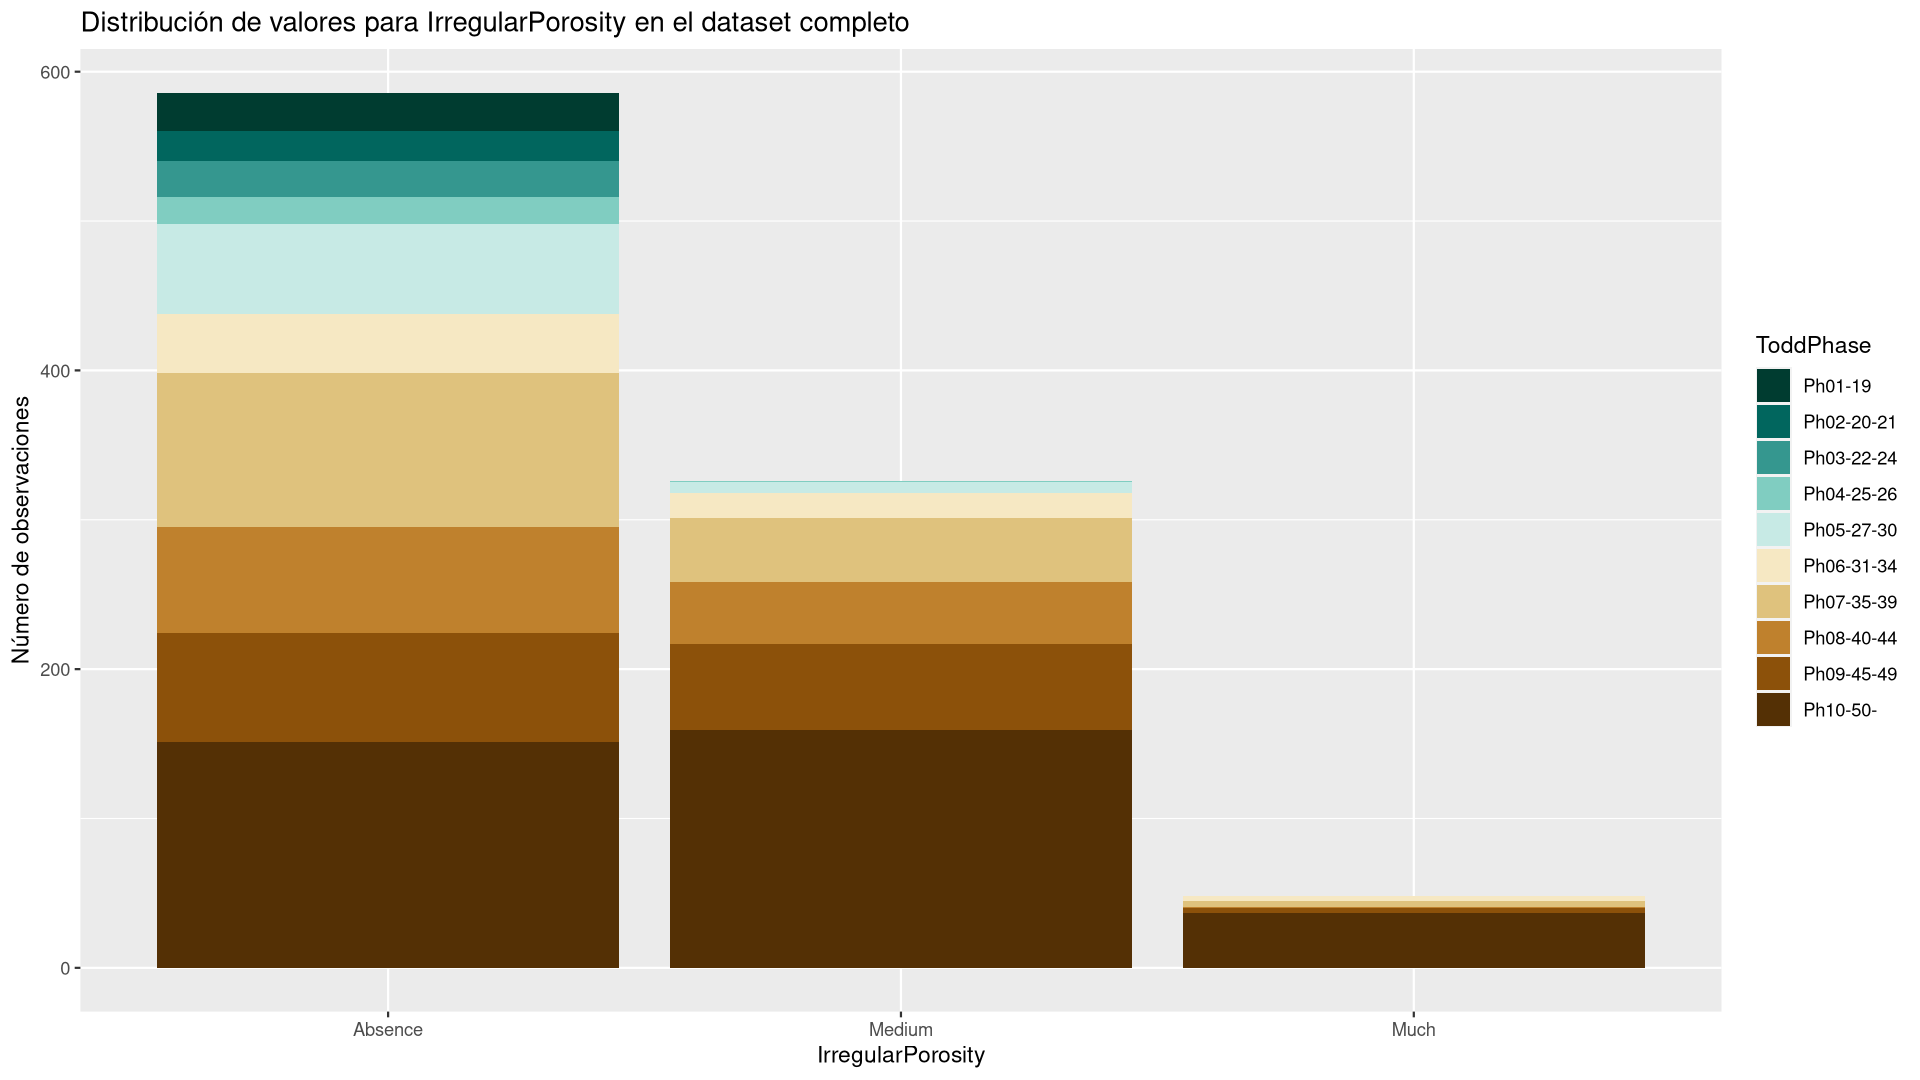
\includegraphics[width = \textwidth]{conjunto_datos/densidad_IrregularPorosity_completo.png}
	\caption{Distribución de los valores de IrregularPorosity en el conjunto de datos completo.}
	\label{fig:densidad_IrregularPorosity_completo}
\end{figure}

\begin{figure}[H]
	\centering
	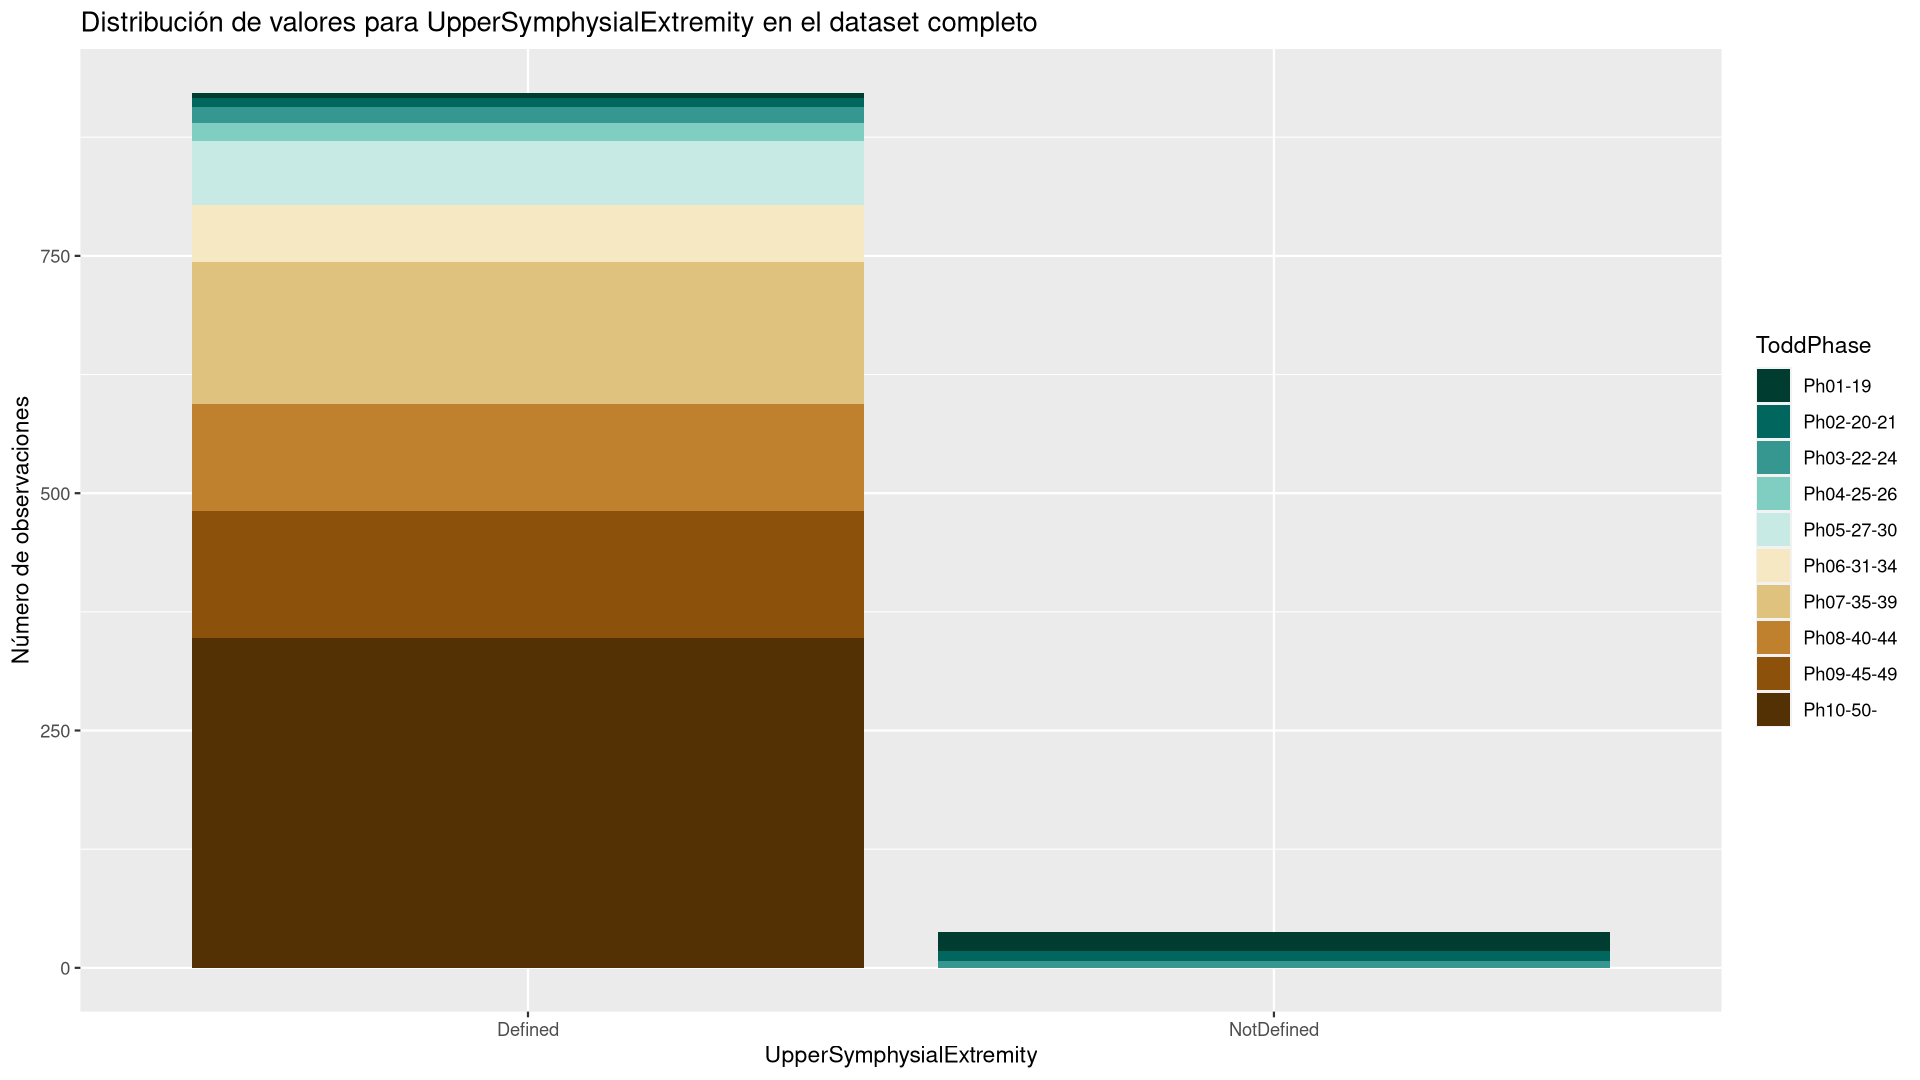
\includegraphics[width = \textwidth]{conjunto_datos/densidad_UpperSymphysialExtremity_completo.png}
	\caption{Distribución de los valores de UpperSymphysialExtremity en el conjunto de datos completo.}
	\label{fig:densidad_UpperSymphysialExtremity_completo}
\end{figure}


\begin{figure}[H]
	\centering
	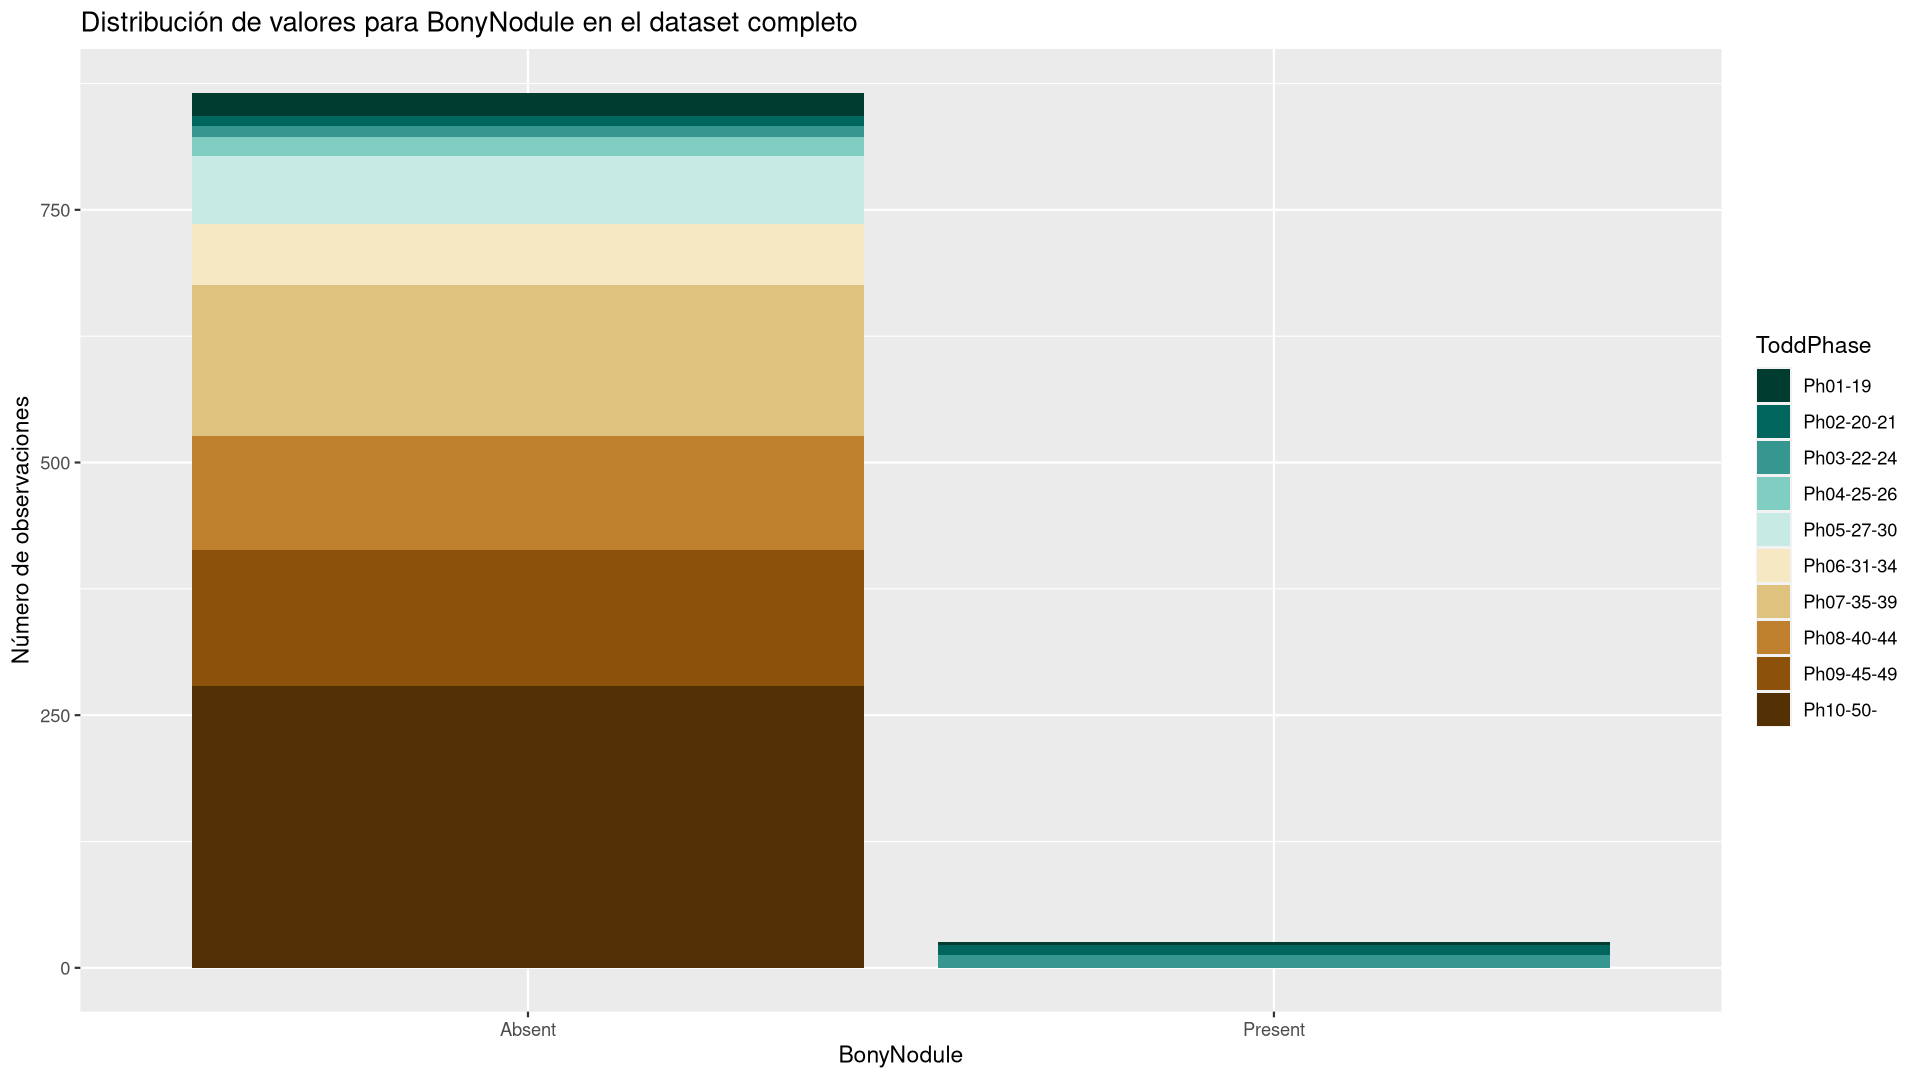
\includegraphics[width = \textwidth]{conjunto_datos/densidad_BonyNodule_completo.png}
	\caption{Distribución de los valores de BonyNodule en el conjunto de datos completo.}
	\label{fig:densidad_BonyNodule_completo}
\end{figure}



\begin{figure}[H]
	\centering
	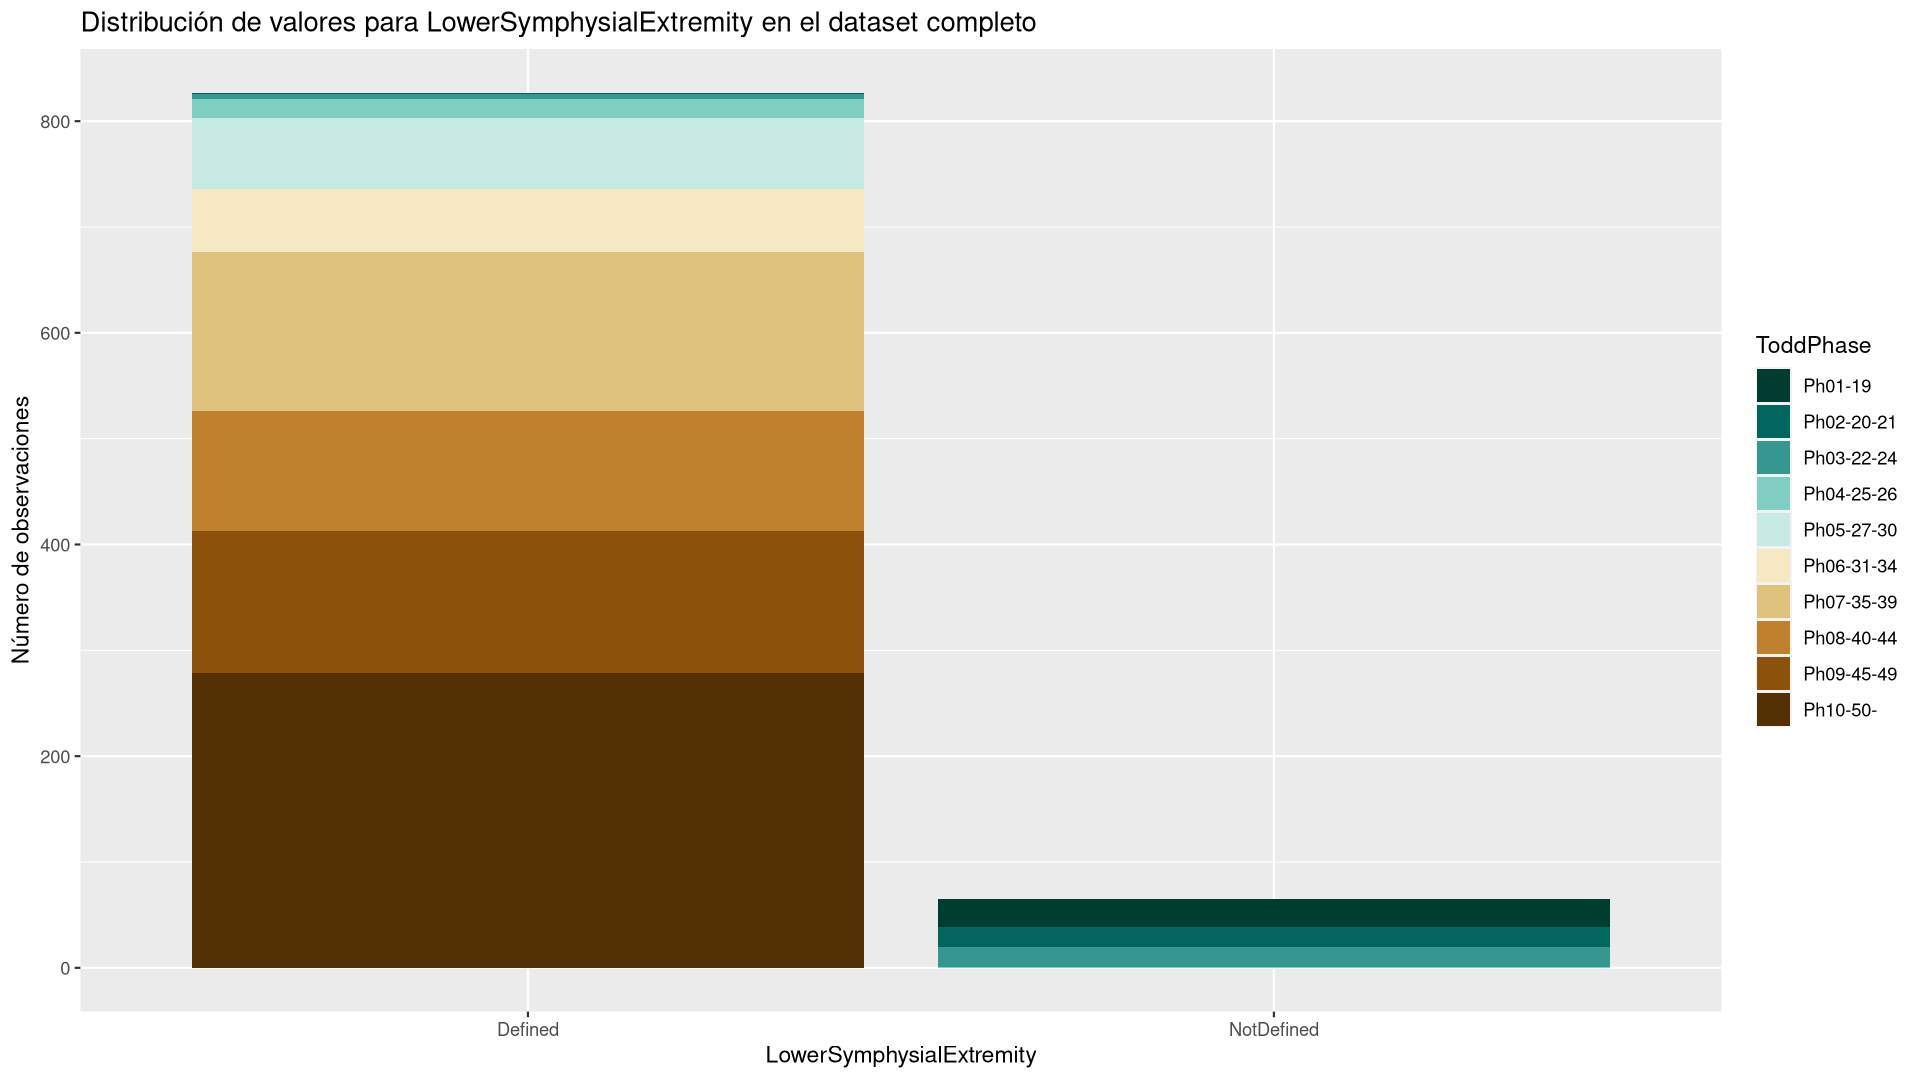
\includegraphics[width = \textwidth]{conjunto_datos/densidad_LowerSymphysialExtremity_completo.png}
	\caption{Distribución de los valores de LowerSymphysialExtremity en el conjunto de datos completo.}
	\label{fig:densidad_LowerSymphysialExtremity_completo}
\end{figure}


\begin{figure}[H]
	\centering
	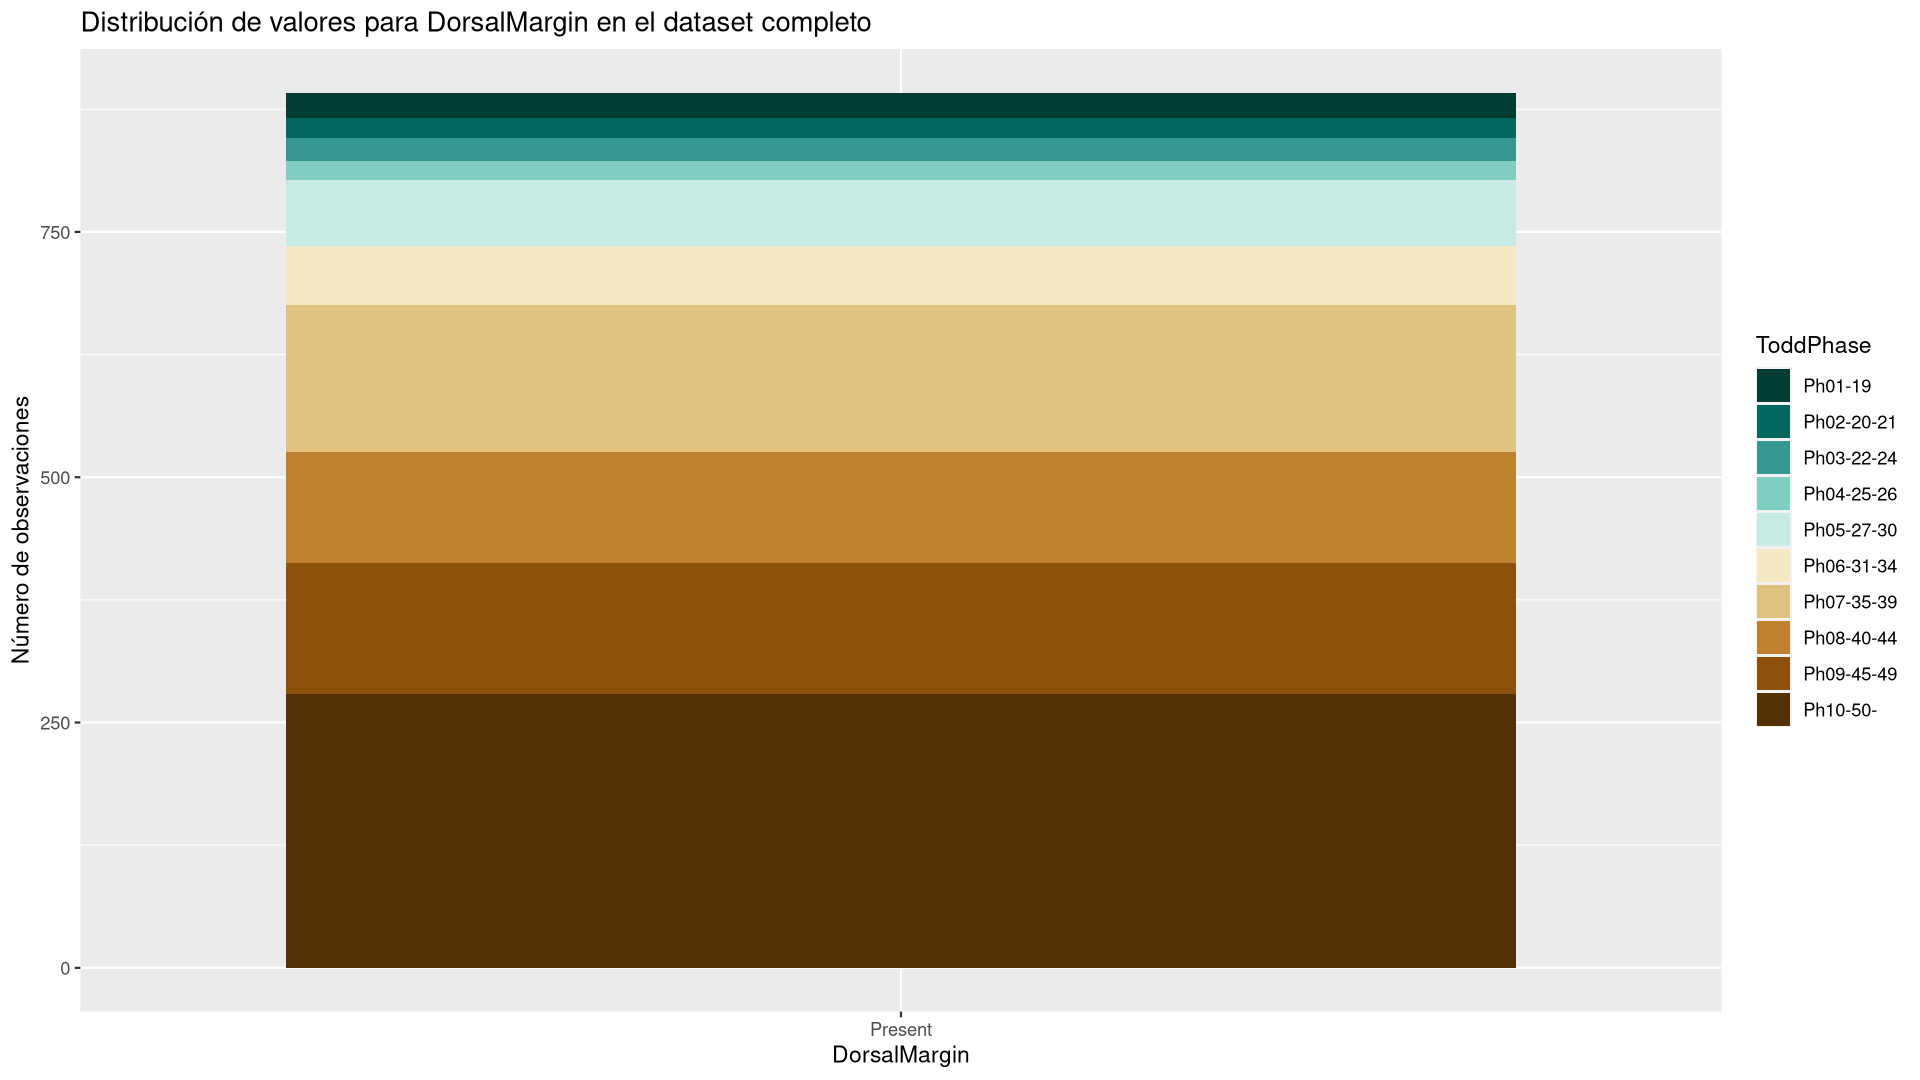
\includegraphics[width = \textwidth]{conjunto_datos/densidad_DorsalMargin_completo.png}
	\caption{Distribución de los valores de DorsalMargin en el conjunto de datos completo.}
	\label{fig:densidad_DorsalMargin_completo}
\end{figure}

En este caso cabe destacar que en todo el conjunto de datos la variable \texttt{DorsalMargin} solo toma el valor de \texttt{Present}, independientemente de la fase a la que pertenezca la observación, por lo que no aporta nada de información a la hora de realizar la clasificación y por lo tanto podemos eliminar este predictor.

\begin{figure}[H]
	\centering
	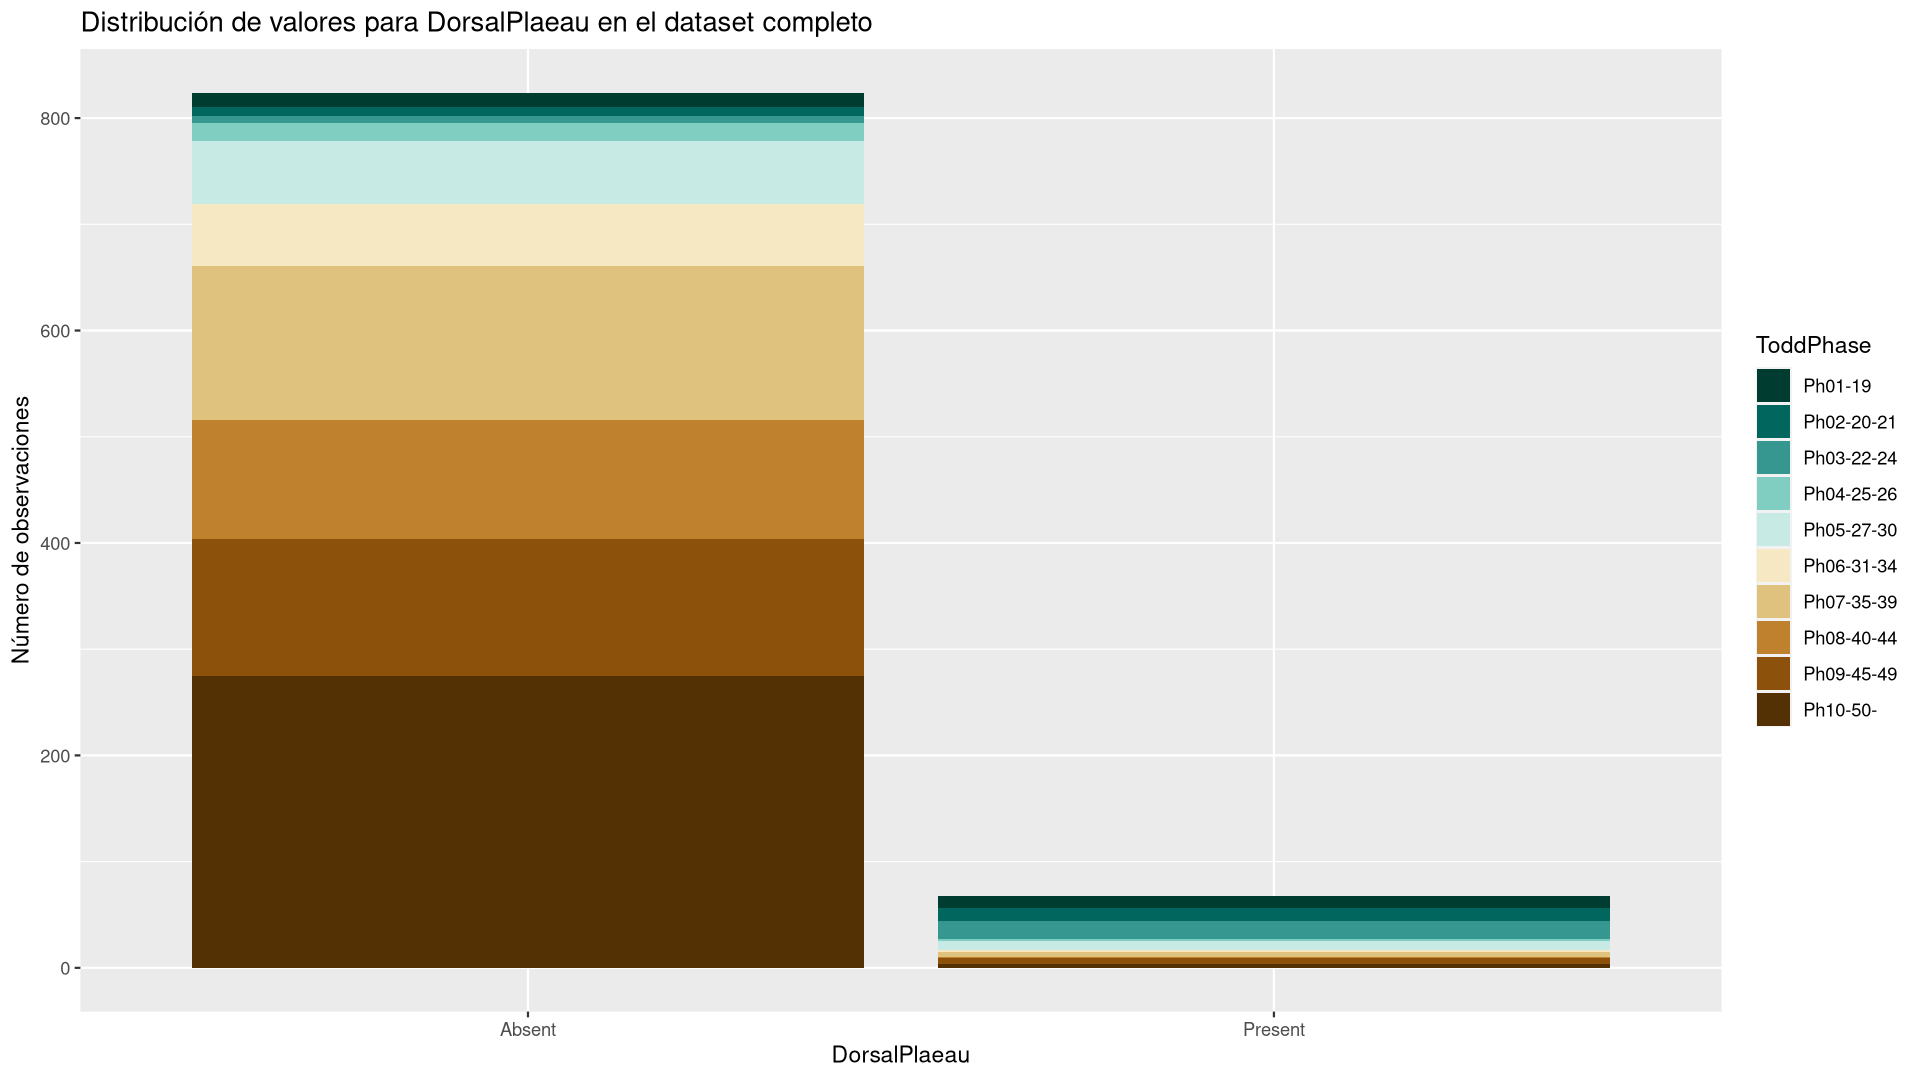
\includegraphics[width = \textwidth]{conjunto_datos/densidad_DorsalPlaeau_completo.png}
	\caption{Distribución de los valores de DorsalPlaeau en el conjunto de datos completo.}
	\label{fig:densidad_DorsalPlaeau_completo}
\end{figure}


\begin{figure}[H]
	\centering
	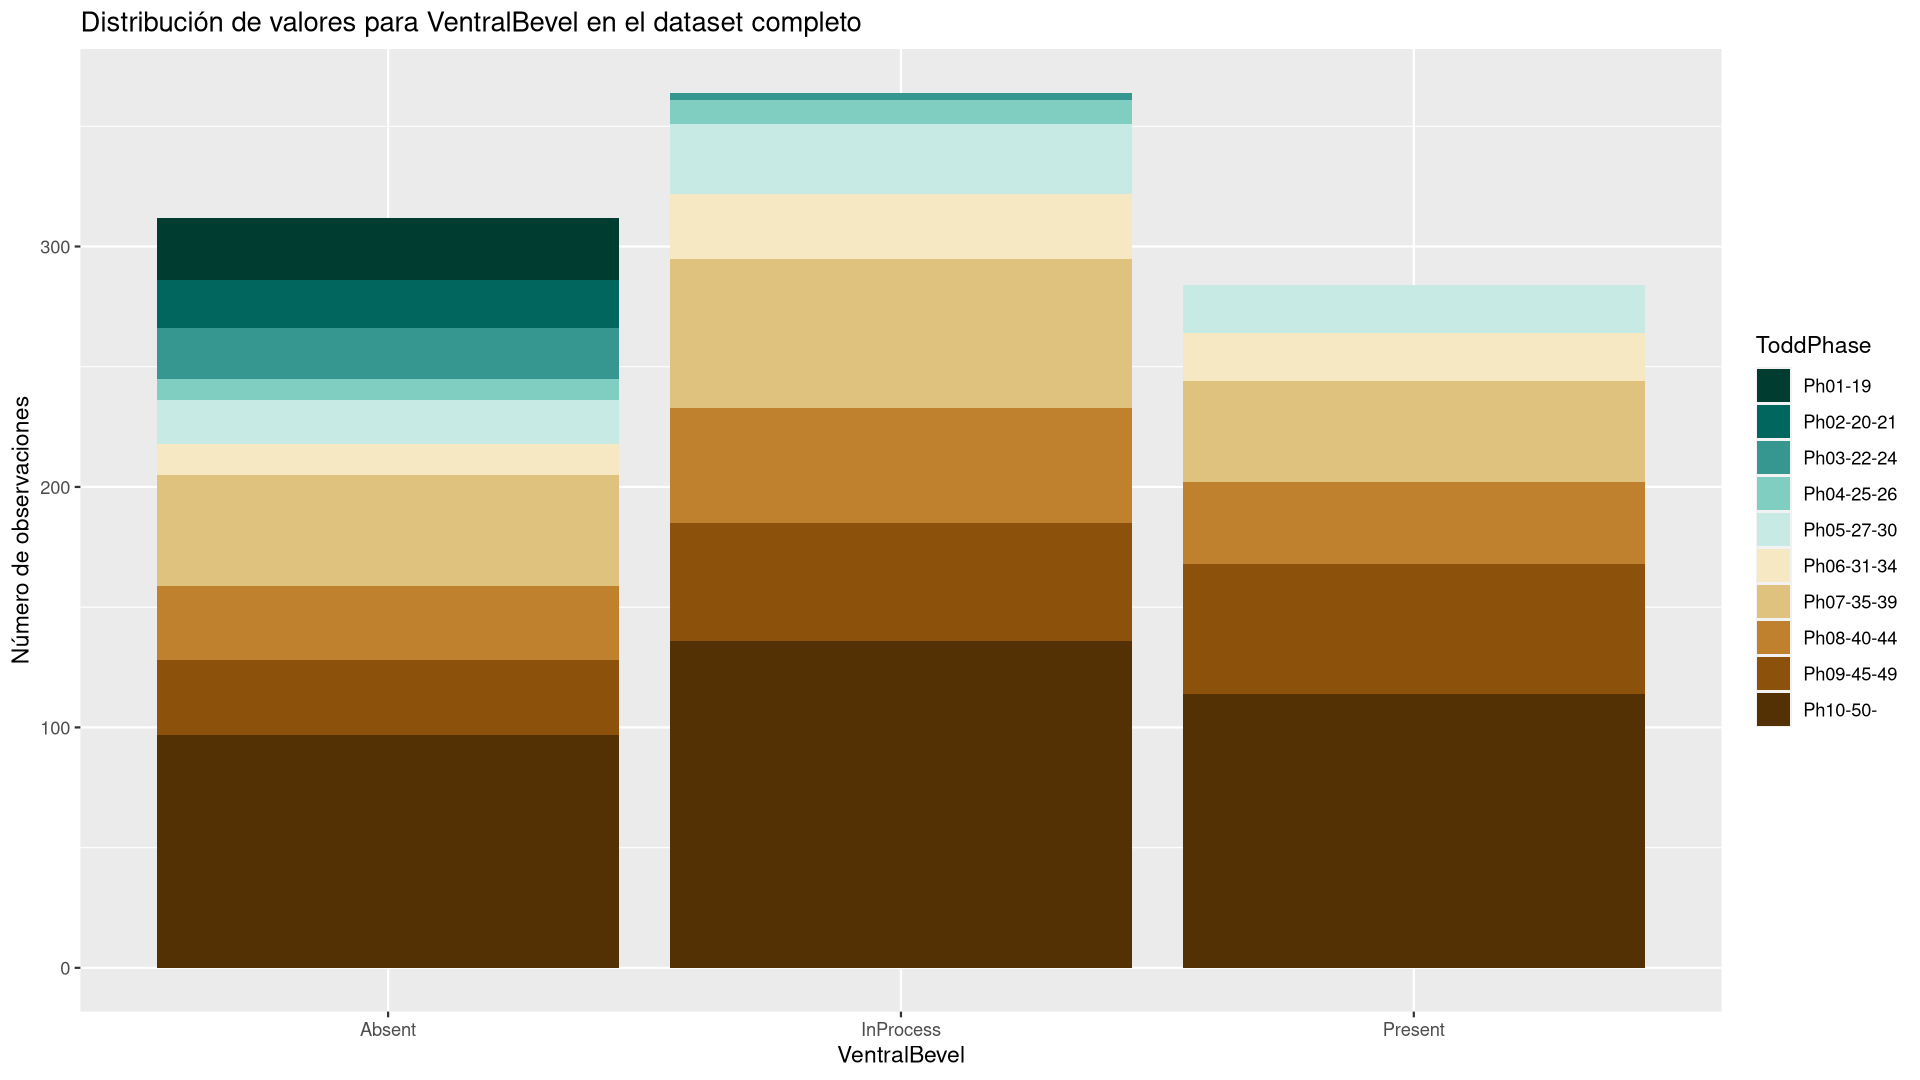
\includegraphics[width = \textwidth]{conjunto_datos/densidad_VentralBevel_completo.png}
	\caption{Distribución de los valores de VentralBevel en el conjunto de datos completo.}
	\label{fig:densidad_VentralBevel_completo}
\end{figure}

\begin{figure}[H]
	\centering
	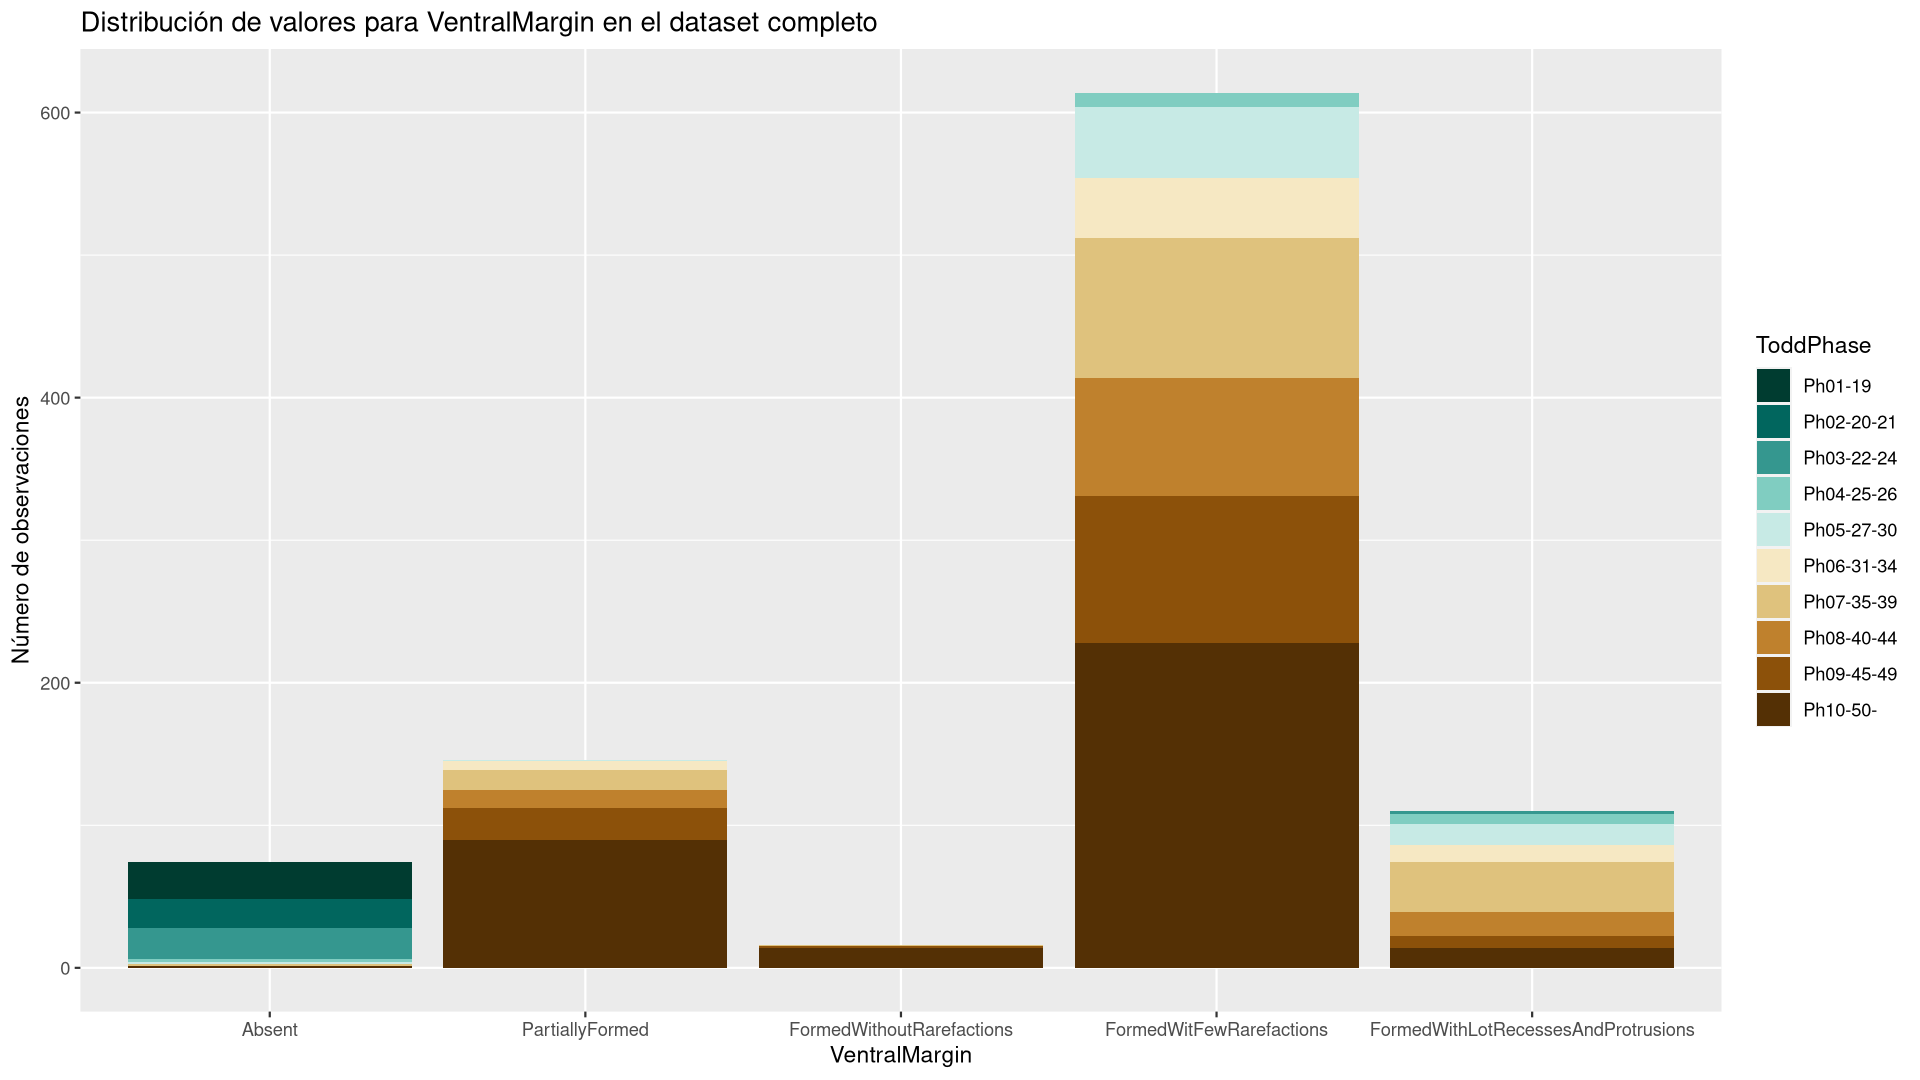
\includegraphics[width = \textwidth]{conjunto_datos/densidad_VentralMargin_completo.png}
	\caption{Distribución de los valores de VentralMargin en el conjunto de datos completo.}
	\label{fig:densidad_VentralMargin_completo}
\end{figure}

% TODO: actualizar toda la parte de sobremuestro, explicando SMOTE, borderline-SMOTE, ADASYN,
% comentar como funciona en nuestro conjunto de datos


\subsubsection{Conclusiones del análisis de datos}

Como breve resumen a este análisis de datos realizado, podemos ver como claramente este problema está desbalanceado y además es de una gran dificultad debido al gran solapamiento entre las clases, haciendo más difícil la clasificación.

También hemos podido observar distintas situaciones donde la decisión de la fase es más clara, acotando el tramo de decisión unicamente a dos o tres fases, sin embargo esto sucede con muy pocas observaciones del conjunto de datos. Hay que recordar que esto se ha hecho con un análisis univariante, es decir, observando por separado cada variable, el modelo que utilicemos tendrá a su disposición cualquier combinación de variables, con lo que se espera encontrar una mayor separabilidad entre las fases de cara a obtener un buen resultado en el problema.

Además, se ha observado que uno de los predictores, \texttt{DorsalMargin}, no aporta información al tomar únicamente un valor para todas las observaciones, independientemente de la clase, por lo que podríamos eliminar esta variable. En caso de no eliminarla, deberíamos observar que o bien no se utiliza en las reglas que obtengamos, o siempre que aparezca el valor utilizado será \texttt{Present}, que es el que siempre toma en el conjunto de datos.

Una vez realizado este análisis de datos, pasamos a las distintas técnicas de preprocesamiento que utilizaremos.


\subsection{Preprocesamiento} \label{sobremuestreo}

En esta sección se discutirá el preprocesamiento a aplicar a los datos de cara a entrenar el modelo, tanto las propias transformaciones que aplicaremos a los datos, como si es necesario aplicar técnicas más avanzadas como sobremuestreo y las algunas propuestas para aplicarlo.

\subsubsection{Transformación de los datos}

Con respecto a las transformaciones de los datos, todo el conjunto de datos está formado por características categóricas, lo que simplificará en gran cantidad tanto la formulación de las reglas como la interpretabilidad, ya que no tendremos que manejar valores reales para las características, en cuyo caso se podría haber propuesto un sistema de reglas difuso. Por este motivo en este caso no será necesario aplicar ninguna transformación a los datos.

Si es cierto que podemos hacer una pequeña selección de características, ya que como hemos visto en el análisis inicial, en concreto en la figura \ref{fig:densidad_DorsalMargin_completo}, la característica \texttt{DorsalMargin} la podemos eliminar del conjunto de datos al no aportar información relevante, al solo tomar un valor.

Tras esto, pasamos a las propuestas para balancear el número de instancias de cada clase.

\subsubsection{Separación en conjunto de entrenamiento y test}

Tras eliminar la característica que no aportaba información, se realizará una separación de los conjuntos de datos en conjuntos de entrenamiento y de test. Esto es importante de cara a la validación del algoritmo, ya que es necesario comprobar que la propuesta se comporta adecuadamente con datos con los que no ha entrenado, aunque dentro de la propia fase de entrenamiento apliquemos una validación cruzada que se explicará más adelante.

Es importante realizar este paso antes de aplicar las técnicas de sobremuestreo para solucionar el balanceo de clases, ya que el conjunto de test no puede contener datos sintéticos, ya que se trata de una prueba real del modelo, como si fueran datos reales que nos han llegado sin etiquetar.

En este caso se ha seleccionado de forma aleatoria uniforme un 80\% de las observaciones del conjunto de datos como datos de entrenamiento y el 20\% restante como datos de test para cada conjunto de datos. Sobre este 80\% de datos serán los datos a los que apliquemos el balanceo de clases, ya que con estos datos son con los que vamos a entrenar el modelo de cara a realizar las predicciones.

\newpage

\subsubsection{Sobremuestreo: Discusión sobre su importancia en este problema}

Ya hemos visto en el análisis de los datos la cantidad de observaciones con las que contamos de cada una de las clases del conjunto de datos \ref{fig:conteo_c}, y observamos como claramente de fases más tempranas apenas tenemos observaciones.

Los conjuntos de datos con esta distribución de observaciones son problemáticos, debido a que cualquier modelo que utilicemos tendrá un sesgo a favor de las clases mayoritarias a la hora de clasificar los datos. Esto se debe a que al realizar la clasificación, cuenta con tan pocos ejemplos de clases minoritarias que simplemente clasificando cualquier observación como de la clase mayoritaria es capaz de obtener un buen resultado de precisión.

Existen varias formas de corregir este problema, dependiendo del enfoque utilizado:

\begin{enumerate}
	\item Adaptando los datos: Se intentan conseguir más muestras de la clase minoritaria, ya sean creados de forma sintética o intentando obtener más información del problema. También se puede reducir el número de observaciones de la clase mayoritaria si contamos con suficientes ejemplos en la clase minoritaria.
	\item Adaptando los algoritmos: Para cada una de las clases se añade un peso de penalización al clasificar erróneamente una observación, de forma que se penaliza más equivocarse al clasificar erróneamente una observación de la clase minoritaria que si el modelo se equivoca en una observación de la clase mayoritaria. Esto en realidad es contrarrestar el sesgo inicial del modelo añadiendo un sesgo manual hacia las clases minoritarias.
\end{enumerate}

En nuestro caso, la primera solución será la que utilicemos debido a que de base el conjunto de datos es pequeño. Utilizaremos sobremuestro ya que no tenemos suficientes datos de las clases minoritarias como para realizar un submuestreo, y eso conllevaría una perdida de información demasiado grande.

% TODO: probar en el algoritmo añadir los pesos para corregir el sesgo
\newpage

\subsubsection{Sobremuestreo: SMOTE}

SMOTE \cite{SMOTE} se trata de un método para conseguir balancear el número de datos para un problema de clasificación creando nuevos datos de las clases minoritarias de forma sintética. Fue propuesto en 2002 por varios investigadores de la Universidad de Florida del sur y la Universidad de Notre Dame.

Su funcionamiento se basa en tomar la clase minoritaria como clase positiva, y para cada elemento de dicha clase positiva buscar los $k$ vecinos más cercanos de la clase positiva. Una vez tenemos los $k$ elementos más cercanos, se crea un dato sintético entre cada vecino seleccionado y el punto original, escogiendo una zona del espacio al azar del segmento que une el vecino seleccionado y el punto original. De esta forma, modificando el número de vecinos a seleccionar, $k$, podemos ajustar el número de nuevos datos sintéticos.

\begin{figure}[H]
	\centering
	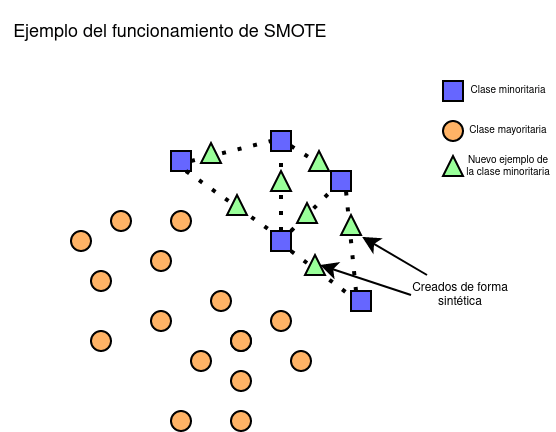
\includegraphics[scale = 0.6]{preprocesamiento/funcionamiento_smote.png}
	\caption{Ilustración de como funciona SMOTE.}
	\label{fig:funcionamiento_smote}
\end{figure}

\newpage

En su propuesta este método fue comparado con otros métodos de sobremuestreo:

\begin{figure}[H]
	\centering
	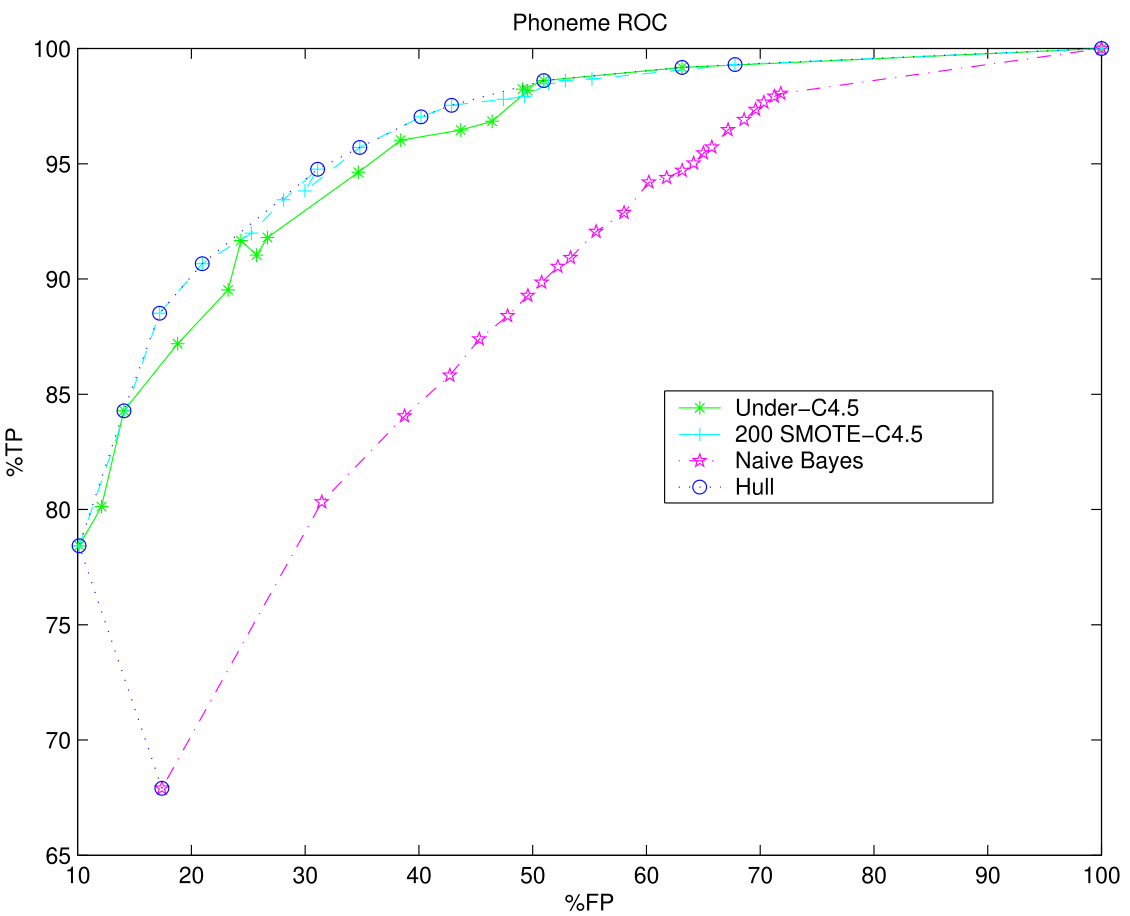
\includegraphics[scale = 1]{preprocesamiento/comparacion_ej_smote.png}
	\caption{Comparación de SMOTE con otros métodos de sobremuestreo en el conjunto de datos Phonome. En el eje X los falsos positivos y en el eje Y los verdaderos positivos. Imagen obtenida de \cite{SMOTE}.}
	\label{fig:comparacionSMOTE}
\end{figure}

Como vemos en la figura \ref{fig:comparacionSMOTE}, este método se comporta bastante bien en comparación con otros métodos y es capaz de obtener buenos resultados, sin embargo, tiene algunos problemas.

Uno de estos problemas es que cuando existe ruido entre las clases, o las clases se encuentran dispersas por el espacio de valores, gran parte de los valores sintéticos se encontrarán en una zona del espacio que no corresponde a su clase.

Este problema se hace mucho más presente en nuestro caso, al contar con tantas clases y con tantas características, y para resolverlo se propuso la variante Borderline-SMOTE.

\subsubsection{Sobremuestreo: Borderline SMOTE}

Borderline SMOTE \cite{BL-SMOTE} se trata de una variante de SMOTE que propone buscar los límites en el espacio de valores de la clase a obtener nuevos datos sintéticos, de forma que cuando se generen dichos datos nuevos, estén dentro de dichos límites. De esta forma evitamos problemas con conjuntos de datos con mucho ruido y múltiples clases.

En su artículo proponen dos variantes, una donde las nuevas muestras sintéticas son creadas a partir de todo el conjunto de datos, y otra donde las nuevas muestras solo se generan a partir de los datos considerados en el límite.


\begin{figure}[H]
    \centering
    \begin{subfigure}[b]{0.33\textwidth}
		  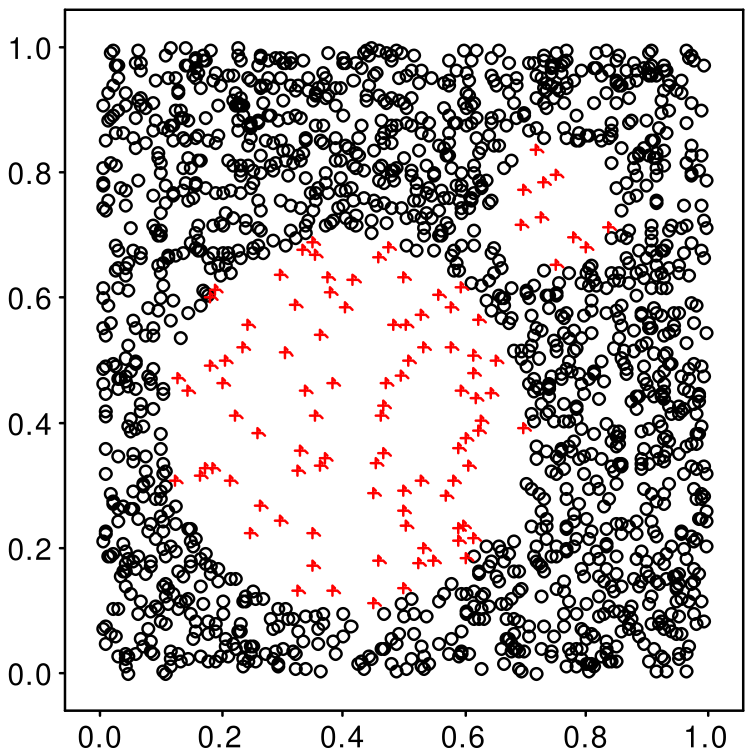
\includegraphics[width=\textwidth]{preprocesamiento/bl-smote-original.png}
        \caption{}
        \label{fig:blSMOTE-orig}
    \end{subfigure}
    \begin{subfigure}[b]{0.33\textwidth}
        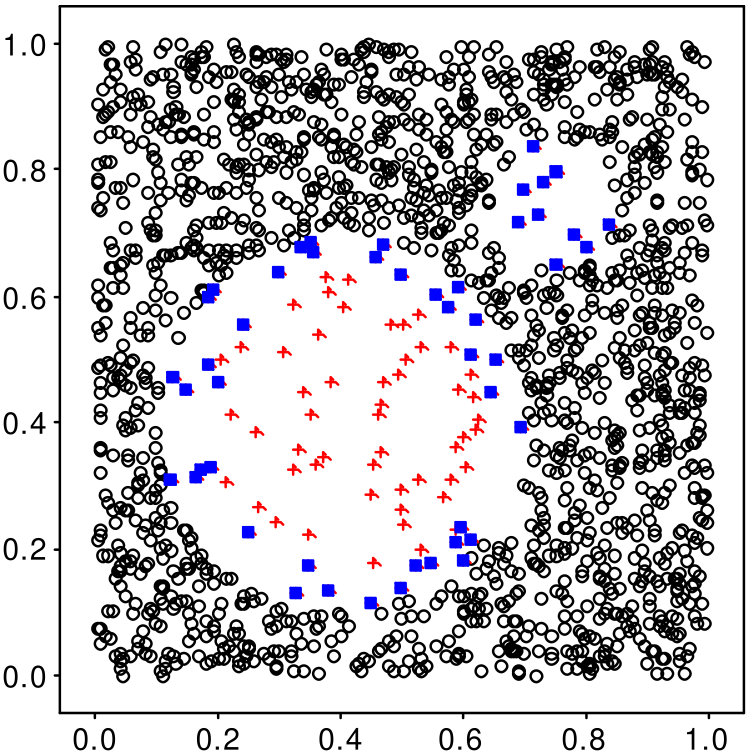
\includegraphics[width=\textwidth]{preprocesamiento/bl-smote-datos-borderline.png}
        \caption{}
        \label{fig:blSMOTE-border}
    \end{subfigure}
    \begin{subfigure}[b]{0.33\textwidth}
        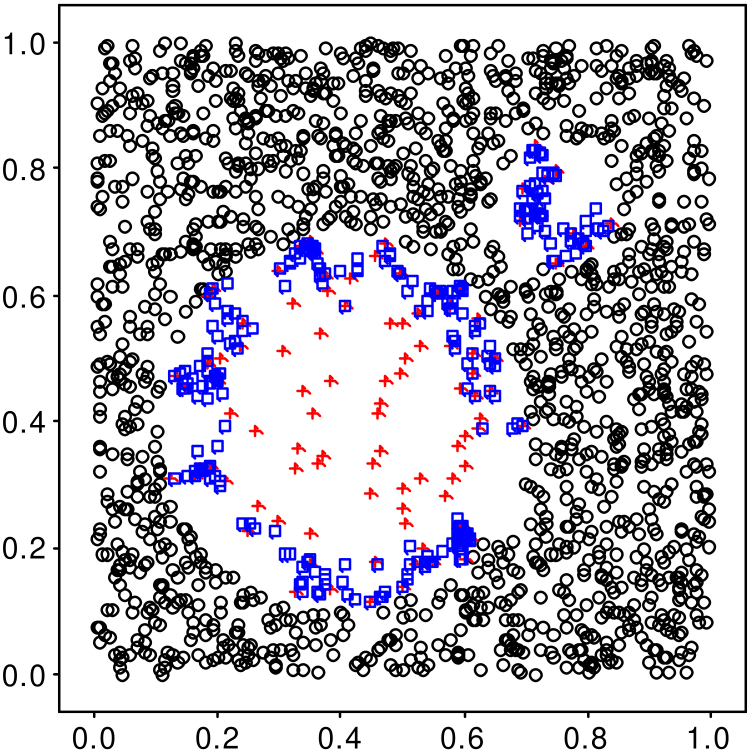
\includegraphics[width=\textwidth]{preprocesamiento/bl-smote-datos-sinteticos.png}
        \caption{}
        \label{fig:blSMOTE-sintetico}
    \end{subfigure}

    \caption{\ref{fig:blSMOTE-orig} Conjunto de datos original. \ref{fig:blSMOTE-border} datos que conforman el límite de la clase minoritaria (cuadros azules rellenos). \ref{fig:blSMOTE-sintetico} Nuevos datos generados de forma sintética dentro de los límites de la clase (cuadros azules no rellenos). Imagen obtenida de \cite{BL-SMOTE}.}
	 \label{fig:ejemploBL-SMOTE}

\end{figure}

Este método funciona de la misma forma que SMOTE a la hora de generar a los nuevos datos sintéticos, sin embargo, lo que hace es en lugar de utilizar todos los datos de la clase minoritaria, hace una preselección de datos, evitando los datos que son considerados como ruido y los datos donde es indiferente crear nuevas observaciones ya que no afectan a la frontera de decisión, es decir, se trata de una zona donde está claro que la clase es minoritaria. Esto hace que los puntos escogidos estén en la zona donde nos interesa tener datos, las fronteras entre las distintas clases, de forma que sea más facil diferenciar una clase de otra. Todo este proceso se ve ilustrado en figura \ref{fig:ejemploBL-SMOTE}.


Para comparar de forma gráfica SMOTE y BorderlineSMOTE podemos observar la siguiente ilustración utilizando datos generados de forma aleatoria con dos dimensiones:

\begin{figure}[H]
    \centering
	 \begin{subfigure}[b]{\textwidth}
		 \centering
		 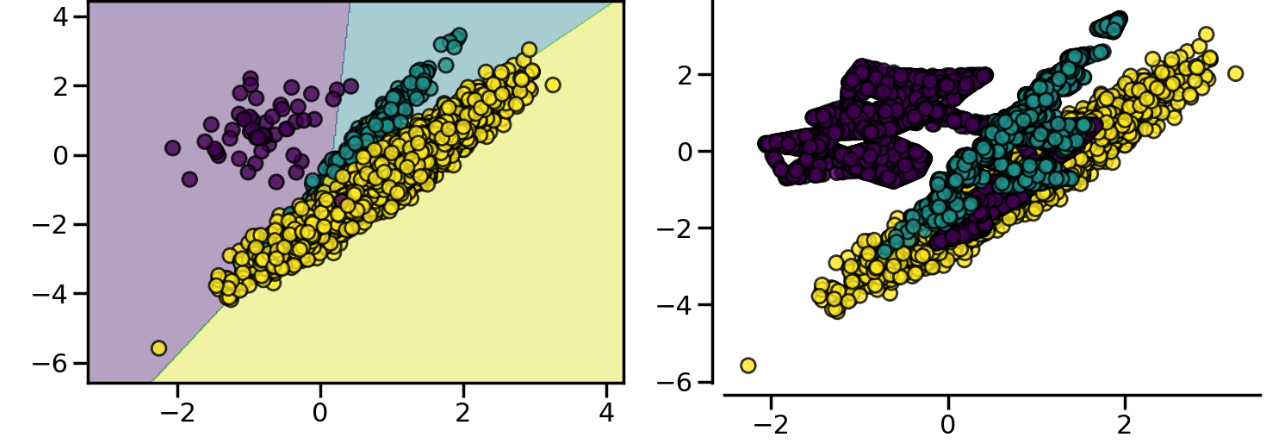
\includegraphics[width=0.8\textwidth]{preprocesamiento/resampling_smote.png}
		 \caption{A la izquierda bordes de las clases, y a la derecha sobremuestreo con SMOTE}
		 \label{fig:SMOTE-cmp}
	 \end{subfigure}

    \begin{subfigure}[b]{\textwidth}
		 \centering
		  \includegraphics[width=0.8\textwidth]{preprocesamiento/resampling_blsmote.png}
        \caption{A la izquierda bordes de las clases, y a la derecha sobremuestreo con BorderlineSMOTE}
        \label{fig:BLSMOTE-cmp}
    \end{subfigure}

    \caption{Comparación de SMOTE y BorderlineSMOTE para un conjunto de datos generado aleatoriamente.}\label{fig:BLSMOTE-SMOTE}

\end{figure}

Esta claro que, como vemos en la figura \ref{fig:ejemploBL-SMOTE} y la figura \ref{fig:BLSMOTE-SMOTE}, esta técnica es mucho más versátil y conveniente que SMOTE.

% TODO: Ampliar a otros métodos de sobremuestreo como ADASYN
% \subsubsection{Sobremuestreo: ADASYN}

\subsubsection{Sobremuestreo: Aplicación sobre datos categóricos}

La propuesta de SMOTE original utiliza el algoritmo k-NN para obtener los vecinos más cercanos, sin embargo, en nuestro caso tenemos un conjunto de datos donde todas las variables son categóricas, y por lo tanto no se puede realizar esta búsqueda de vecinos.

Para solucionar este problema utilizaremos la propuesta de SMOTE-N \cite{SMOTE}, también propuesta en el mismo trabajo donde se propuso SMOTE. Esta propuesta se basa en modificar el algoritmo k-NN utilizado en SMOTE por el k-NN propuesto por Stanfill y Waltz en 1986 \cite{kNNSMOTEN}, donde para aplicar el k-NN a un conjunto de datos categóricos utilizaban una versión modificada de la métrica de diferencia de valor, donde la distancia se basaba en el grado de diferencia entre los valores categóricos.

Por otro lado, BorderlineSMOTE no propone ninguna modificación para solucionar este problema, sin embargo como las características de nuestro conjunto de datos toman valores ordenados, como por ejemplo el nivel de porosidad, o el nivel de surcos presentes, se han codificado los datos de forma ordinal, transformando cada observación a un vector de enteros, asignando un entero a cada nivel de los valores que pueden tomar para cada una de sus características. Con esta modificación hemos podido aplicar BorderlineSMOTE y después deshacer la codificación para obtener los resultados del sobremuestreo con las etiquetas originales.

\subsection{Análisis de datos tras el preprocesado}

Como vimos en la sección de análisis del conjunto de datos, vamos a analizar los datos obtenidos tanto por SMOTE como por Borderline SMOTE. Debido a la similitud entre ambas lateralidades, en esta ocasión solo comentaremos los efectos que podemos ver en el conjunto de datos completo. Este análisis nos servirá para observar si la aplicación de estas técnicas de sobremuestreo ha funcionado para equilibrar el número de clases, y si ha tenido algún efecto negativo que podamos ver utilizando la información de cada variable por separado, como añadir ruido o solape a las clases aplicar estas técnicas.

\subsubsection{Análisis del conjunto completo tras aplicar SMOTE}


\begin{figure}[H]
	\centering
	\includegraphics[width = \textwidth]{conjunto_datos_smote/distribucion_clases_completo_SMOTE.png}
	\caption{Número de datos por cada fase propuesta por Todd con el conjunto de datos completo.}
	\label{fig:conteo_c_smote}
\end{figure}

Como era de esperar, claramente se han balanceado el número de observaciones de cada clase, como era de esperar. Un detalle a tener en cuenta es que SMOTE no ha sido capaz de generar tantas instancias de las otras clases como la clase mayoritaria, por lo que ha tenido que hacer un submuestreo para esta clase, pasando la última fase de 279 observaciones a 222 observaciones.

\begin{figure}[H]
	\centering
	\includegraphics[width = \textwidth]{conjunto_datos_smote/densidad_IrregularPorosity_completo_SMOTE.png}
	\caption{Distribución de los valores de IrregularPorosity en el conjunto de datos completo.}
	\label{fig:densidad_IrregularPorosity_completo_smote}
\end{figure}

Para \texttt{IrregularPorosity} vemos como ahora para el valor \texttt{Absence} todas las fases tienen un número de observaciones similar, cuando antes aunque existían observaciones de todas las clases con este valor, las de la fase cuatro al ser tan minoritaria podría pasar desapercibida. Por otro lado vemos como el número de observaciones con valor \texttt{Medium} casi se ha duplicado, pero manteniendo las observaciones que vimos anteriormente, este valor solo lo toman observaciones de fases altas. Esto último también ha ocurrido con el valor \texttt{Much}.

\begin{figure}[H]
	\centering
	\includegraphics[width = \textwidth]{conjunto_datos_smote/densidad_UpperSymphysialExtremity_completo_SMOTE.png}
	\caption{Distribución de los valores de UpperSymphysialExtremity en el conjunto de datos completo.}
	\label{fig:densidad_UpperSymphysialExtremity_completo_smote}
\end{figure}

Con \texttt{UpperSymphysialExtremity} de nuevo vuelve a ocurrir que la distribución de las fases para valores de \texttt{Defined} se equilibra, al añadir más instancias de las clases minoritarias, sin embargo hay que tener en cuenta que cuanto más baja es la fase, menos observaciones aparecen y más pasan al valor \texttt{NotDefined}, luego la aplicación de SMOTE nos ha confirmado que aunque algunas observaciones de fases bajas toman el valor de \texttt{Defined}, esto no es lo común y suelen tomar el valor de \texttt{NotDefined}.

\begin{figure}[H]
	\centering
	\includegraphics[width = \textwidth]{conjunto_datos_smote/densidad_BonyNodule_completo_SMOTE.png}
	\caption{Distribución de los valores de BonyNodule en el conjunto de datos completo.}
	\label{fig:densidad_BonyNodule_completo_smote}
\end{figure}

En el caso de \texttt{BonyNodule} vuelve a ocurrir lo mismo que con \texttt{UpperSymphysialExtremity} pero con la segunda y tercera fase.


\begin{figure}[H]
	\centering
	\includegraphics[width = \textwidth]{conjunto_datos_smote/densidad_LowerSymphysialExtremity_completo_SMOTE.png}
	\caption{Distribución de los valores de LowerSymphysialExtremity en el conjunto de datos completo.}
	\label{fig:densidad_LowerSymphysialExtremity_completo_smote}
\end{figure}

Con \texttt{LowerSymphysialExtremity} se vuelve a repetir lo comentado anteriormente, pero en este caso dejando todavía más claro que el valor \texttt{NotDefined} solo lo toman valores de la primera y segunda fase, mientras que existe algo de solape entre \texttt{Defined} y \texttt{NotDefined} en la tercera fase, y de la cuarta fase en adelante siempre toma el valor de \texttt{Defined}.

\begin{figure}[H]
	\centering
	\includegraphics[width = \textwidth]{conjunto_datos_smote/densidad_DorsalPlaeau_completo_SMOTE.png}
	\caption{Distribución de los valores de DorsalPlaeau en el conjunto de datos completo.}
	\label{fig:densidad_DorsalPlaeau_completo_smote}
\end{figure}

Observando como se ha comportado SMOTE con \texttt{DorsalPlaeau} podemos sacar unas conclusiones más interesantes. Al principio parecía que este predictor no aportaba información debido a que tanto con \texttt{Absent} como con \texttt{Present} había observaciones de todas las clases, sin embargo tras aplicar SMOTE podemos ver como ha encontrado muchos más vecinos de las tres primeras clases con valor \texttt{Present} que con \texttt{Absent}, mientras que el resto de clases no ha encontrado vecinos con los que aumentar el número de observaciones con \texttt{Present}, haciendo que ahora este valor sea mayormente indicador de que la observación se encuentra en las tres primeras fases.

\begin{figure}[H]
	\centering
	\includegraphics[width = \textwidth]{conjunto_datos_smote/densidad_VentralBevel_completo_SMOTE.png}
	\caption{Distribución de los valores de VentralBevel en el conjunto de datos completo.}
	\label{fig:densidad_VentralBevel_completo_smote}
\end{figure}

Para \texttt{VentralBevel}, como con otros predictores, con SMOTE ha mantenido lo que observamos al analizar los datos originales. Si se toma el valor de \texttt{InProcess} y en especial \texttt{Present} es indicador de que la observación se trata de una fase alta.


\begin{figure}[H]
	\centering
	\includegraphics[width = \textwidth]{conjunto_datos_smote/densidad_VentralMargin_completo_SMOTE.png}
	\caption{Distribución de los valores de VentralMargin en el conjunto de datos completo.}
	\label{fig:densidad_VentralMargin_completo_smote}
\end{figure}

Por último, para la variable \texttt{VentralMargin} es para la única que se ha modificado muy notablemente la distribución de clases con respecto a los valores que toma la característica. Empezando por lo que esperábamos, para el valor \texttt{Absent} siguen siendo observaciones de fases tempranas. Para \texttt{PartiallyFormed}, lo que en principio parecía un poco de solape de la quinta fase, pero nos dejaba bastante claro que se trataban de observaciones de la fase seis en adelante, ha pasado a ser una distribución de observaciones equitativa entre todas las fases de la cuarta a la décima, esto se puede explicar debido a la falta de observaciones, que muchas de estas al tomar otros valores de \texttt{VentralMargin} no disponiamos de la información suficiente para saber que en realidad también forma parte de \texttt{PartiallyFormed}. Lo mismo sucede con \texttt{FormedWithoutRarefactions}, lo que parecía una clara clasificación a la última fase debido a la falta de muestras ahora no está tan claro, al haber encontrado vecinos más cercanos de otras fases con este valor. De nuevo, con \texttt{FormedWithFewRarefactions} pasa al contrario, y parece ser que el detalle del submuestreo comentado en el número de observaciones por cada clase se ha realizado para observaciones con este valor, aunque con las otras características no es visible a simple vista, aquí esta claro, al pasar de casi seiscientas observaciones a menos de cincuenta. Esto puede ser debido a que al aplicar el proceso de búsqueda de vecinos sea la zona donde menos vecinos ha podido encontrar, decidiendo eliminar observaciones de esta zona.

\newpage


\subsubsection{Análisis del conjunto completo tras aplicar BorderlineSMOTE}

Debido a que las soluciones para BorderlineSMOTE son muy parecidas a nivel gráfico que las de SMOTE, no se han añadido las imágenes para no extender de forma innecesaria el análisis, debido a que se sacarían las mismas conclusiones.

Lo importante de aplicar este algoritmo sería si las observaciones generadas realmente se encuentran en una zona crucial de la frontera de decisión, sin embargo esto no lo podemos observar de forma gráfica al contar con demasiadas dimensiones.

\subsubsection{Conclusiones de la aplicación de sobremuestreo}


Como conclusiones comentar que, a priori, con este pequeño análisis de datos, parece que estas técnicas de sobremuestreo pueden ayudar a la hora de entrenar el modelo.

La aplicación de estas técnicas nos puede ayudar a reafirmar la utilidad de ciertos valores para decidir la fase o al menos acotarla, por lo que podría disminuir el sesgo del modelo sin haber añadido información errónea. La única excepción a esto puede ser con la última característica, \texttt{VentralMargin}, donde si hemos visto una gran diferencia entre el conjunto original y el conjunto con sobremuestreo, aunque esto puede ser tanto por falta de información en el conjunto completo, o porque realmente ha añadido información incorrecta en este caso.



\newpage


\section{Programación Genética}

Programación Genética es un tipo de algoritmo evolutivo, inspirado en la evolución biológica y sus mecanismos principales. Antes de comentar las principales particularidades de Programación Genética explicaremos en que se basan los algoritmos evolutivos.

\subsection{Bases de algoritmos evolutivos}

Los algoritmos evolutivos son algoritmos que utilizan los mecanismos la evolución biológica, para intentar optimizar soluciones a un problema dado. Este tipo de algoritmos surgen tras diversas propuestas a finales de la década de 1950 \cite{historiaAlgoritmosEvolutivos} donde se proponen utilizar mecanismos basados en la biología para aplicarlos a máquinas de Turing. Tras estas propuestas, en la década de 1960 Hans-Joachim Bremermann desarrollo lo que sería la teoría de los algoritmos evolutivos.

\subsubsection{Funcionamiento de los algoritmos evolutivos}

La idea principal de este tipo de algoritmos es utilizar una población de individuos que serán soluciones al problema, de forma que aplicando ciertos mecanismos como la reproducción, mutación, recombinación, elitismo y selección la población evolucione hacia mejores soluciones. Estas soluciones se evaluarán utilizando una función objetivo que será la función a minimizar o maximizar.

El funcionamiento básico de este tipo de algoritmos es el siguiente:

\begin{enumerate}
	\item Generar una población inicial.
	\item Repetir hasta la condición de parada:
	\begin{enumerate}
		\item Evaluar la población actual para la función objetivo.
		\item Seleccionar los individuos que generarán la próxima generación.
		\item Aplicar la reproducción, mutación o recombinación de los individuos seleccionados, generando la población de hijos.
		\item Reemplazar la población de hijos por la población actual (con elitismo si así se quiere).
	\end{enumerate}
\end{enumerate}

Estos pasos generales son los que todo algoritmo evolutivo suele seguir, aunque existen muchas variantes. La condición de parada puede variar dependiendo de que se busque conseguir, puede ser, por ejemplo, que se realicen cierto número de evaluaciones de la población, o que se consiga cierto valor mínimo de la función objetivo.

Los distintos operadores de mutación, reproducción o recombinación no siempre son aplicados. Cada uno de estos eventos tendrá cierta probabilidad, de forma que el proceso será en parte aleatorio. Normalmente la recombinación o reproducción serán muy comunes, mientras que la mutación será más atípica.


\subsubsection{Modelos de población en algoritmos evolutivos}

También podemos hacer dos distinciones claras a la hora de como funcionan las poblaciones de este tipo de algoritmos:

\begin{itemize}
	\item Modelo de población generacional (figura \ref{fig:modelo_generacioal}): En este modelo la población es reemplazada por completo en cada iteración, de forma que se tienen que generar tantos hijos como elementos tiene la población.
	\item Modelo de población estacionario (figura \ref{fig:modelo_estacionario}): En este modelo solo se generan dos hijos, y esos dos hijos compiten por entrar en la población, reemplazando a los dos peores individuos de esta.
\end{itemize}

\begin{figure}[H]
    \centering
	  \includegraphics[width=\textwidth]{generacional.png}
    \caption{Esquema de un algoritmo evolutivo con un modelo generacional.}
	 \label{fig:modelo_generacioal}
\end{figure}

\begin{figure}[H]
    \centering
	  \includegraphics[width=\textwidth]{estacionario.png}
    \caption{Esquema de un algoritmo evolutivo con un modelo estacionario.}
	 \label{fig:modelo_estacionario}
\end{figure}


\subsubsection{Principales paradigmas de algoritmos evolutivos}

Existen cuatro enfoques básicos de algoritmos evolutivos.

\begin{enumerate}
	\item Estrategias de Evolución.
	\item Programación Evolutiva.
	\item Algoritmos Genéticos.
	\item Programación Genética.
\end{enumerate}

El primer enfoque, Estrategias de Evolución, es desarrollado por Hans-Paul Schwefel e Ingo Rechenberg a partir de 1964 y presentado en 1971 como su tesis doctoral \cite{estrategiasEvolucion}. En este trabajo se enfatiza en como los individuos de la población realizan sus cambios, haciendo un análisis más exhaustivo en como aplicar los cambios a los individuos, y no en su representación como tal.

El segundo enfoque, Programación Evolutiva, fue propuesto por Lawrence J. Fogel en 1966 \cite{programacionEvolutiva}, y es de los primeros trabajos donde se propone un algoritmos basado en algoritmos evolutivos y la teoría desarrollada por Bremermann.

El tercer enfoque, Algoritmos Genéticos, propuesto en 1975 por John Holland, de la Universidad de Michigan, en su libro publicado ese mismo año \cite{libroAlgoritmosGeneticos}. Este enfoque se basaba en dar a los elementos de la población una representación en cromosomas, de forma que se aplicaban operadores genéticos sobre dichos cromosomas para hacerlos evolucionar y mejorar su valor de la función objetivo.

El último enfoque, Programación Genética, es el que utilizaremos, y se explicará más en detalle en los siguientes apartados.


\subsection{Como funciona Programación Genética}

Programación Genética fue impulsada por John Koza a comienzos de la década de 1990 \cite{kozaGP}. Este enfoque de algoritmo evolutivo se basa en utilizar expresiones en forma de árbol como individuos de la población. Con esta representación en árbol se puede llegar a entrenar desde fórmulas matemáticas o lógicas, hasta programas escritos en C o cualquier otro lenguaje de programación cuya gramática se pueda expresar como un árbol.

\begin{figure}[H]
    \centering
	 \begin{subfigure}[b]{0.49\textwidth}
		 \centering
		 \includegraphics[width=0.5\textwidth]{arbol_exp_matematica.png}
		 \caption{Expresión matemática $4 \cdot ( (-x / 2) + y)$ representada como un árbol.}
		 \label{fig:exp_matematica}
	 \end{subfigure}
	 \begin{subfigure}[b]{0.49\textwidth}
		 \centering
		\includegraphics[width=0.5\textwidth]{arbol_exp_logica.png}
		\caption{Expresión lógica $ a \wedge (\neg (b \vee c) ) $ representada como un árbol.}
		\label{fig:exp_logica}
   \end{subfigure}
	\caption{Algunos ejemplos de expresiones representadas como árboles.}
	\label{fig:arbol_exp}
\end{figure}

Como podemos imaginar, estos árboles no son de un tamaño ni profundidad fijas, si no que el tamaño de los individuos será variable, a diferencia de los cromosomas utilizados en Algoritmos Genéticos.

También tenemos que tener en cuenta que en este caso evaluar la población requiere recorrer cada árbol por completo de forma recursiva, por lo que esto será una operación bastante costosa.

De cara a funcionar con expresiones en forma de árbol, los operadores de Programación Genética deben tener en cuenta esta estructura.

\subsection{Operadores de Programación Genética}

\subsubsection{Operador de cruce}

El operador de cruce de Programación Genética se trata de una recombinación de subárboles escogidos de forma aleatoria.

\begin{figure}[H]
    \centering
	 \begin{subfigure}[b]{\textwidth}
		 \centering
		 \includegraphics[width=0.5\textwidth]{cruce_GP.png}
		 \caption{Dos expresiones a cruzar.}
		 \label{fig:cruce_GP}
	 \end{subfigure}

	\begin{subfigure}[b]{\textwidth}
		 \centering
		\includegraphics[width=0.5\textwidth]{cruce_GP_seleccion.png}
		\caption{Selección aleatoria de los subárboles a cruzar.}
		\label{fig:cruce_GP_seleccion}
   \end{subfigure}

	\begin{subfigure}[b]{\textwidth}
		\centering
	  \includegraphics[width=0.5\textwidth]{cruce_GP_final.png}
	  \caption{Expresiones tras realizar el cruce.}
	  \label{fig:cruce_GP_final}
   \end{subfigure}

	\caption{Ejemplo del operador de cruce en dos árboles.}
	\label{fig:ej_cruce_GP}
\end{figure}

Como vemos en la figura \ref{fig:ej_cruce_GP}, se trata simplemente de escoger dos puntos al azar en el árbol e intercambiar los respectivos subárboles, aunque esto puede acarrear problemas ya que podríamos llegar a tener árboles excesivamente grandes.

\subsubsection{Operador de mutación}

El operador de mutación puede tener dos comportamientos. Este operador escogerá un punto al azar del árbol, y puede:

\begin{enumerate}
	\item Reemplazar de forma aleatoria el valor del nodo actual (siempre por un nodo del mismo tipo) (figura \ref{fig:mutacion_suave}).
	\item Reemplazar el subárbol a partir del punto escogido (figura \ref{fig:mutacion_fuerte}).
\end{enumerate}

\begin{figure}[H]
    \centering
	 \begin{subfigure}[b]{0.49\textwidth}
		 \centering
		 \includegraphics[width=0.5\textwidth]{arbol_mutar.png}
		 \caption{Expresión a mutar.}
		 \label{fig:arbol_mutar}
	 \end{subfigure}
	\begin{subfigure}[b]{0.49\textwidth}
		 \centering
		\includegraphics[width=0.5\textwidth]{punto_mutacion.png}
		\caption{Selección aleatoria del punto a mutar.}
		\label{fig:punto_mutacion}
   \end{subfigure}

	\begin{subfigure}[b]{0.49\textwidth}
		\centering
	  \includegraphics[width=0.5\textwidth]{mutacion_suave.png}
	  \caption{Expresiones tras realizar la mutación de tipo 1.}
	  \label{fig:mutacion_suave}
   \end{subfigure}
	\begin{subfigure}[b]{0.49\textwidth}
		\centering
	  \includegraphics[width=0.5\textwidth]{mutacion_fuerte.png}
	  \caption{Expresiones tras realizar la mutación de tipo 2.}
	  \label{fig:mutacion_fuerte}
	\end{subfigure}

	\caption{Ejemplo del operador de mutación sobre un individuo.}
	\label{fig:ej_mutacion_GP}
\end{figure}

En este caso el segundo tipo de mutación nos ofrece una mayor diversidad en las expresiones y por eso es la que se suele utilizar, aunque cabe mencionar que el propio operador de cruce ya añade suficiente diversidad y por este motivo la mutación no es tan importante en Programación Genética.


\subsection{Elitismo}

En este algoritmo también se podrá aplicar elitismo. Tras evaluar la población de hijos se buscará el mejor individuo de la población anterior, y si no está presente en la nueva población generada se introducirá, de cara a mantener el mejor individuo si este no ha sido seleccionado como padre o si los hijos derivados de este conforman una solución peor.


\subsection{Problemas de Programación Genética}

También tenemos que tener en cuenta que, por como funciona Programación Genética y sus operadores, existen algunos problemas con este algoritmo.

\subsubsection{Sobreajuste en el tamaño de los árboles}

Uno de los problemas principales en todos los modelos de Aprendizaje Automático es el sobreajuste de un modelo a los datos con los que se entrena.

En Programación Genética este problema se acentúa, ya que la estructura utilizada, los árboles, pueden variar su tamaño, y por lo tanto crecer tanto como sea necesario para ajustarse lo máximo posible a los datos de entrenamiento.

De cara a evitar esto se suele utilizar una longitud máxima para los árboles, de forma que todo operador que se aplique a un árbol ha de asegurar que dicha longitud máxima no se ha sobrepasado.

\subsubsection{Aprendizaje de constantes numéricas}

Programación Genética utilizará como variables de entrada las características del conjunto de datos que queramos entrenar, sin embargo aplicará operaciones matemáticas a dichas características y será necesario utilizar valores constantes para obtener la salida deseada como etiqueta.

Esto será uno de los problemas de Programación Genética, ya que, por ejemplo, si de forma aleatoria no se obtienen los valores deseados se deberán realizar esas operaciones con las constantes actuales, llenando gran parte de la expresión de operaciones entre constantes, que en realidad podrían ser un único nodo.

Este problema se ha solucionado de distintas formas, desde propuestas de modificaciones a Programación Genética como veremos más adelante, o aplicando algún tipo de búsqueda de mínimos (como una búsqueda local) a las constantes numéricas cada ciertas iteraciones del algoritmo.


\newpage


\section{Implementación}

Respecto a la implementación, el software para balancear las clases está implementado en Python mientras que las ejecuciones experimentales se han realizado en R utilizando la biblioteca RKEEL.

% TODO: Explicar el algoritmo de Bojarczuk_GP

\subsubsection{Otras funciones auxiliares}

También disponemos de algunas funciones auxiliares, que nos servirán a lo largo de todo el código, como la comprobación de si dos valores reales son iguales teniendo en cuenta los problemas de representación de números en coma flotante de C++, o distintas posibles funciones de evaluación que hemos predefinido.

\newpage

\subsection{Validación de las pruebas}


Uno de los problemas que nos encontramos en los algoritmos de aprendizaje automático es la validación del algoritmo, es decir, como podemos asegurar que nuestro algoritmo realmente funciona, y no se trata de que ha hecho un sobreajuste con los datos con los que ha entrenado y fuera de dichos datos no es capaz de realizar buenas predicciones.

Para comprobar y asegurarnos que los algoritmos son capaces de realizar buenas predicciones fuera de los datos con los que ha entrenado utilizaremos validación cruzada con $k$ iteraciones.

Este método consiste en dividir el conjunto de entrenamiento en $k$ partes de mismo tamaño, de forma que realizaremos $k$ iteraciones para entrenar nuestro modelo. En cada iteración utilizaremos una de estas partes como conjunto de validación y las otras $k - 1$ partes como conjunto de entrenamiento, de forma que el algoritmo no haya entrenado con esa parte de validación. Finalmente para obtener el error del algoritmo para dicho conjunto de datos utilizaremos la media del error en los distintos conjuntos de validación de cada iteración.

Es importante destacar que antes de hacer las separaciones en $k$ subconjuntos de datos el conjunto de entrenamiento se reordenará de forma aleatoria para evitar que un conjunto en el que los datos estén ordenados por clase se excluya del entrenamiento cierta clase, porque todas sus muestras están en el conjunto de validación.

De esta forma podremos obtener un valor del error del algoritmo para unos datos con los que no ha entrenado, a la vez que comprobamos que nuestro algoritmo es capaz de ajustarse bien o no a un conjunto de datos.


\begin{figure}[H]
    \centering

	 \begin{subfigure}[b]{\textwidth}
		\centering
		\includegraphics[width=0.8\textwidth]{cross_validation/conjunto_datos.png}
		\caption{Ejemplo de un conjunto de 16 datos.}
	  \label{fig:ej_16_datos}
   \end{subfigure}
	\vspace{1cm}

	 \begin{subfigure}[b]{\textwidth}
		 \centering
		 \includegraphics[width=0.8\textwidth]{cross_validation/iteracion1.png}
 		 \caption{Separación entre validación y entrenamiento en la primera iteración.}
 	    \label{fig:cv_iteracion1}
	 \end{subfigure}
	 \vspace{1cm}

	\begin{subfigure}[b]{\textwidth}
		 \centering
		 \includegraphics[width=0.8\textwidth]{cross_validation/iteracion2.png}
 		 \caption{Separación entre validación y entrenamiento en la segunda iteración.}
 	    \label{fig:cv_iteracion2}
   \end{subfigure}
	\vspace{1cm}

	\begin{subfigure}[b]{\textwidth}
		 \centering
		 \includegraphics[width=0.8\textwidth]{cross_validation/iteracion3.png}
 		 \caption{Separación entre validación y entrenamiento en la tercera iteración.}
 	    \label{fig:cv_iteracion3}
	\end{subfigure}
	\vspace{1cm}

	\begin{subfigure}[b]{\textwidth}
		 \centering
		 \includegraphics[width=0.8\textwidth]{cross_validation/iteracion4.png}
 		 \caption{Separación entre validación y entrenamiento en la cuarta iteración.}
 	    \label{fig:cv_iteracion4}
	\end{subfigure}

	\caption{Ejemplo de validación cruzada de 4 iteraciones.}
	\label{fig:4-cv-ejemplo}
\end{figure}


\subsubsection{Validación cruzada utilizando 5x2cv}

En nuestro caso utilizaremos 5x2cv para validación. Este método fue propuesto por Thomas G. Dietterich en el año 1998 \cite{propuesta5x2cv}.

Este método se basa en realizar cinco repeticiones de una validación cruzada con dos iteraciones, cada una de estas repeticiones utilizando particiones distintas de los datos al 50\%. De esta forma, con cada una de las cinco particiones que realicemos a los datos aplicaremos una validación cruzada con dos folds, entrenando con la primera mitad de los datos y validando con la segunda mitad en el primer fold, y al contrario en el segundo fold.

Como podemos ver, con cinco repeticiones y siendo cada una de estas un 2-cv (de ahí el nombre 5x2cv) obtendremos diez valores de error, siendo el error final obtenido en validación la media de estos diez valores.



\newpage

\subsection{Funciones de evaluación}

De cara a evaluar los algoritmos necesitaremos una función de evaluación que nos permita saber el error que estamos cometiendo en las estimaciones.

En nuestro caso, al estar ante un problema de clasificación utilizaremos las siguientes:

\begin{itemize}
	\item Precisión.
	\item Área bajo la curva ROC.
	\item Error absoluto medio ordinal.
\end{itemize}

\subsubsection{Precisión}


\subsubsection{Área bajo la curva ROC}


\subsubsection{Error absoluto medio ordinal}



\newpage

\subsection{Documentación del proyecto}

Todo el proyecto se ha documentado con Doxygen, y se puede acceder a la documentación a través del fichero \texttt{index.html} de la carpeta \texttt{docs/} en el código o bien en la web \url{https://advy99.github.io/algoritmos_poblacion_expresiones/}, ya que se ha utilizado la herramienta GitHub Pages \cite{GHPages} para alojar la documentación del proyecto.

En este documento se puede encontrar la estructura del proyecto, así como las distintas opciones de compilación.

\begin{figure}[H]
	 \centering
	 \includegraphics[width=\textwidth]{documentacion.png}
	 \caption{Página principal de la documentación del proyecto.}
	\label{fig:documentación}
\end{figure}

\newpage

\subsection{Verificación del software desarrollado}

De cara a verificar que las distintas clases y métodos desarrollados funcionan utilizaremos GoogleTest \cite{gtest}.

GoogleTest es un entorno de trabajo para verificar software a través de test unitarios.

Los test unitarios son test que evalúan una sección concreta de un software, con el objetivo de comprobar que dicha sección de código funciona de forma correcta, y de esta forma aislar las secciones de código que no se comportan como esperábamos, facilitando la tarea de prueba y corrección de errores en un código.

Para que estos tests nos sean útiles tienen que cumplir las siguientes condiciones:

\begin{enumerate}
	\item Tienen que ser independientes y repetibles. El resultado de un test no debe depender de otros test, de forma que si un test falla este falle por la sección de código que estamos probando, no porque existe un test que no se comporta como creíamos.
	\item Tienen que estar estructurados, y reflejar como funciona todo el conjunto del software. De esta forma es sencillo separar como funcionan las distintas partes del software, permitiendo centrarnos en comprobar que cada parte funciona de forma correcta.
	\item Deben de ser portables y reutilizables. Los tests deben finalizar correctamente independientemente del sistema y compilador utilizado.
	\item Cuando un test falla debe proporcionar tanta información como le sea posible.
	\item Los test han de ser rápidos. El objetivo es comprobar que el software funciona como queremos de una forma rápida, sin perder más tiempo en ejecutar los tests que en compilar y ejecutar el sistema.
\end{enumerate}

Siguiendo estas premisas, se han diseñado tests para cada una de las clases y el conjunto del sistema software. Dichos tests están disponibles en la carpeta \texttt{test} del software, y además el fichero para generar el software ejecutará dichos tests, de forma que si estos tests no son completados correctamente detendrá la compilación.

\newpage

\subsection{Como utilizar y compilar el software}

Existen diversas formas de compilar, todas ellas utilizando el comando `make`.

\begin{itemize}
	\item Sin parámetros (\texttt{make}): Compilar con optimización y utilizando OpenMP para añadir paralelismo.
	\item Target \texttt{test} (\texttt{make test}): Compilar los test de GTest.
	\item Target \texttt{doc} (\texttt{make doc}): Compilar la documentación.
	\item Target \texttt{clean} (\texttt{make clean}): Limpiar los objetos tras una compilación.
	\item Variable \texttt{OPTIMIZACION} (\texttt{make OPTIMIZACION=3}): Por defecto 3, asignar un nivel de compilación. Los posibles valores son 0, 1, 2, 3 y g.
	\item Variable \texttt{OPENMP} (\texttt{make OPENMP=1}): Por defecto 1. Activar o desactivar la compilación con OpenMP, 0 desactivado, 1 activado.
	\item Variable \texttt{DEBUG} (\texttt{make DEBUG=0}): Por defecto 0. Activar o desactivar la compilación con símbolos de depuración.
	\item Variable \texttt{GPROF} (\texttt{make GPROF=0}): Por defecto 0. Activar o desactivar la compilación con GPROF de cara a hacer profiling al software.

\end{itemize}

Siempre que se compile se recompilará la documentación, de cara a posibles cambios.

Todas las variables se pueden combinar, por ejemplo, es posible cambiar el nivel de optimización y a la vez desactivar OpenMP.

Los binarios se generarán en la carpeta \texttt{bin} y cada uno de ellos tiene instrucciones de como utilizarlos.

\newpage

\subsection{Ejecución con un conjunto de datos de prueba}

De cara a probar que nuestra implementación funciona vamos a utilizar un conjunto de datos sencillo, con pocos datos y cuyo funcionamiento es muy simple, Iris \cite{irisDataset}. Este dataset contiene tres características de tres variantes de la flor Iris: Setosa, Versicolour y Virginica. Existen 50 muestras de cada clase, siendo 150 muestras en total.

% TODO: lanzar iris como conjunto de prueba


\newpage

\subsection{Uso de paralelismo}

Una de las tareas más costosas que nos podemos encontrar en ambos algoritmos es evaluar la población cuando esta tiene un gran número de individuos y el número de datos es muy elevado.

Para reducir el tiempo utilizado por estas tareas podemos aprovechar el paralelismo de los datos. Evaluar una expresión es totalmente independiente de evaluar otra, de forma que esta tarea se puede realizar en paralelo y así reducir el tiempo de ejecución.

También se ha probado el paralelizar la generación de la nueva población en cada generación del algoritmo, ya que en las operaciones de cruce y mutación son independientes entre sí al seleccionar a priori que elementos formarán parte del cruce y mutación, sin embargo esto no ha dado buenos resultados ya que el coste de crear y eliminar los hilos que se ejecutarán en paralelo, sumado a las esperas en secciones críticas esto hacía que el tiempo de ejecución fuera igual o superior a ejecutarlo en secuencial.

\newpage


\section{Resultados} \label{resultados}

De cara a comentar los resultados, vamos a recordar el entorno de experimentación utilizad. Para comenzar, se ha dividido el conjunto de datos original en un 80\% para entrenamiento y un 20\% para test, luego, tras esa separación, se ha aplicado sobremuestreo al conjunto de entrenamiento, sin modificar el conjunto de test, y ya en la ejecución de los algoritmos se ha utilizado una validación cruzada de 5 folds (5-cv) sobre el conjunto de entrenamiento, mientras que el conjunto de test que aparece en estos resultados es siempre el mismo, el 20\% original sin sobremuestreo, aplicado sobre el clasificador obtenido en cada fold.

La sección se dividirá en tres apartados, uno por conjunto de datos utilizado:

\begin{enumerate}
	\item Conjunto con sobremuestreo aleatorio.
	\item Conjunto con sobremuestro usando SMOTE.
	\item Conjunto con sobremuestro usando BL-SMOTE.
\end{enumerate}

Dentro de cada una de estas secciones habrá otro apartado para cada uno de los algoritmos utilizados:

\begin{enumerate}
	\item Algoritmo de Bjorczuk.
	\item Algoritmo de Falco.
	\item Algoritmo de Tan.
\end{enumerate}

\subsection{Resultados con sobremuestreo aleatorio}

\subsubsection{Algoritmo de Bjorczuk original}


\begin{table}[H]
\centering
\resizebox{\textwidth}{!}{%
\begin{tabular}{|ccccccc|}
\hline
\multicolumn{7}{|c|}{\textbf{\begin{tabular}[c]{@{}c@{}}Resultados de Bjorczuk con sobremuestreo aleatorio y función\\ de fitness por defecto.\end{tabular}}}                                                                                                             \\ \hline
\multicolumn{1}{|c|}{\multirow{2}{*}{}} & \multicolumn{3}{c|}{\textbf{OMAE}}                                                                                        & \multicolumn{3}{c|}{\textbf{Accuracy}}                                                              \\ \cline{2-7}
\multicolumn{1}{|c|}{}                  & \multicolumn{1}{c|}{\textbf{Training}} & \multicolumn{1}{c|}{\textbf{Validacion}} & \multicolumn{1}{c|}{\textbf{Test}}    & \multicolumn{1}{c|}{\textbf{Training}} & \multicolumn{1}{c|}{\textbf{Validacion}} & \textbf{Test}   \\ \hline
\multicolumn{1}{|c|}{\textbf{Fold 1}}   & \multicolumn{1}{c|}{2,5189}           & \multicolumn{1}{c|}{2,5053}             & \multicolumn{1}{c|}{\textbf{2,5219}} & \multicolumn{1}{c|}{0,1}               & \multicolumn{1}{c|}{0,1}                 & 0,0677          \\ \hline
\multicolumn{1}{|c|}{\textbf{Fold 2}}   & \multicolumn{1}{c|}{3,0986}           & \multicolumn{1}{c|}{3,0964}             & \multicolumn{1}{c|}{3,1068}          & \multicolumn{1}{c|}{0,1009}            & \multicolumn{1}{c|}{0,1018}              & 0,1198          \\ \hline
\multicolumn{1}{|c|}{\textbf{Fold 3}}   & \multicolumn{1}{c|}{3,0982}            & \multicolumn{1}{c|}{3,1}                  & \multicolumn{1}{c|}{3,1083}          & \multicolumn{1}{c|}{0,1014}            & \multicolumn{1}{c|}{0,1}                 & 0,1198          \\ \hline
\multicolumn{1}{|c|}{\textbf{Fold 4}}   & \multicolumn{1}{c|}{4,5}                & \multicolumn{1}{c|}{4,5}                  & \multicolumn{1}{c|}{4,5}               & \multicolumn{1}{c|}{0,1}               & \multicolumn{1}{c|}{0,1}                 & \textbf{0,3594} \\ \hline
\multicolumn{1}{|c|}{\textbf{Fold 5}}   & \multicolumn{1}{c|}{3,1004}           & \multicolumn{1}{c|}{3,0963}             & \multicolumn{1}{c|}{3,1058}           & \multicolumn{1}{c|}{0,1013}            & \multicolumn{1}{c|}{0,1036}              & 0,1198          \\ \hline
\multicolumn{1}{|c|}{\textbf{Media}}   & \multicolumn{1}{c|}{3,2632}           & \multicolumn{1}{c|}{3,2596}             & \multicolumn{1}{c|}{3,2685}           & \multicolumn{1}{c|}{0,1007}            & \multicolumn{1}{c|}{0,1010}              & 0,1573          \\ \hline
\end{tabular}%
}
\caption{Tabla de resultados de Bjorczuk sobre el conjunto con sobremuestreo aleatorio.}\label{tablaBJORCZUKdefecto}
\end{table}



Si nos fijamos en los resultados, vemos que los resultados de tasa de precisión en entrenamiento y validación es del 10\%. Si vemos la matriz de confusión obtenida esto se debe a que el algoritmo se está centrando solo en una de las diez clases, y clasifica todas las instancias siempre con la misma clase, también de ahí la gran variación en el valor de la tasa de acierto, si la clase en la que siempre clasifica es, por ejemplo, la clase 10, la fase de mayores de 50, como en el caso del cuarto fold, obtenemos una tasa muy alta, sin embargo, si se centra en una clase central, como el fold 1 que clasifica todas las instancias como la quinta fase, obtiene una tasa de acierto mucho menor. Esto se debe a que en el conjunto de test, a diferencia del conjunto de entrenamiento, al no estar balanceadas las clases obtiene un valor de tasa de acierto mucho más alto en el cuarto fold, al centrarse en la fase donde más observaciones tenemos.

Por este motivo, es importante también observar el OMAE, ya que en este problema tan complejo nos puede resultar más interesante el hecho de que nos equivoquemos en clases cercanas, aunque nos equivoquemos de clase.


\begin{table}[H]
\centering
\resizebox{\textwidth}{!}{%
\begin{tabular}{|ccccccccccccc|}
\hline
\multicolumn{13}{|c|}{\textbf{\begin{tabular}[c]{@{}c@{}}Matriz de confusión obtenida en el fold 4 sobre el conjunto de test con el algoritmo \\ de Bjorczuk con sobremuestreo aleatorio y función de fitness por defecto.\end{tabular}}}                                                                                                                                                              \\ \hline
\multicolumn{2}{|c|}{\multirow{2}{*}{}}                                               & \multicolumn{10}{c|}{\textbf{Clase predicha}}                                                                                                                                                                                                                              & \multirow{2}{*}{} \\ \cline{3-12}
\multicolumn{2}{|c|}{}                                                                & \multicolumn{1}{c|}{C0} & \multicolumn{1}{c|}{C1} & \multicolumn{1}{c|}{C2} & \multicolumn{1}{c|}{C3} & \multicolumn{1}{c|}{C4} & \multicolumn{1}{c|}{C5} & \multicolumn{1}{c|}{C6} & \multicolumn{1}{c|}{C7} & \multicolumn{1}{c|}{C8} & \multicolumn{1}{c|}{C9}          &                   \\ \hline
\multicolumn{1}{|c|}{\multirow{10}{*}{\textbf{Clase real}}} & \multicolumn{1}{c|}{C0} & \multicolumn{1}{c|}{0}  & \multicolumn{1}{c|}{0}  & \multicolumn{1}{c|}{0}  & \multicolumn{1}{c|}{0}  & \multicolumn{1}{c|}{0}  & \multicolumn{1}{c|}{0}  & \multicolumn{1}{c|}{0}  & \multicolumn{1}{c|}{0}  & \multicolumn{1}{c|}{0}  & \multicolumn{1}{c|}{\textbf{5}}  & C0 = Ph01-19      \\ \cline{2-13}
\multicolumn{1}{|c|}{}                                      & \multicolumn{1}{c|}{C1} & \multicolumn{1}{c|}{0}  & \multicolumn{1}{c|}{0}  & \multicolumn{1}{c|}{0}  & \multicolumn{1}{c|}{0}  & \multicolumn{1}{c|}{0}  & \multicolumn{1}{c|}{0}  & \multicolumn{1}{c|}{0}  & \multicolumn{1}{c|}{0}  & \multicolumn{1}{c|}{0}  & \multicolumn{1}{c|}{\textbf{4}}  & C1 = Ph02-20-21   \\ \cline{2-13}
\multicolumn{1}{|c|}{}                                      & \multicolumn{1}{c|}{C2} & \multicolumn{1}{c|}{0}  & \multicolumn{1}{c|}{0}  & \multicolumn{1}{c|}{0}  & \multicolumn{1}{c|}{0}  & \multicolumn{1}{c|}{0}  & \multicolumn{1}{c|}{0}  & \multicolumn{1}{c|}{0}  & \multicolumn{1}{c|}{0}  & \multicolumn{1}{c|}{0}  & \multicolumn{1}{c|}{\textbf{5}}  & C2 = Ph03-22-24   \\ \cline{2-13}
\multicolumn{1}{|c|}{}                                      & \multicolumn{1}{c|}{C3} & \multicolumn{1}{c|}{0}  & \multicolumn{1}{c|}{0}  & \multicolumn{1}{c|}{0}  & \multicolumn{1}{c|}{0}  & \multicolumn{1}{c|}{0}  & \multicolumn{1}{c|}{0}  & \multicolumn{1}{c|}{0}  & \multicolumn{1}{c|}{0}  & \multicolumn{1}{c|}{0}  & \multicolumn{1}{c|}{\textbf{4}}  & C3 = Ph04-25-26   \\ \cline{2-13}
\multicolumn{1}{|c|}{}                                      & \multicolumn{1}{c|}{C4} & \multicolumn{1}{c|}{0}  & \multicolumn{1}{c|}{0}  & \multicolumn{1}{c|}{0}  & \multicolumn{1}{c|}{0}  & \multicolumn{1}{c|}{0}  & \multicolumn{1}{c|}{0}  & \multicolumn{1}{c|}{0}  & \multicolumn{1}{c|}{0}  & \multicolumn{1}{c|}{0}  & \multicolumn{1}{c|}{\textbf{13}} & C4 = Ph05-27-30   \\ \cline{2-13}
\multicolumn{1}{|c|}{}                                      & \multicolumn{1}{c|}{C5} & \multicolumn{1}{c|}{0}  & \multicolumn{1}{c|}{0}  & \multicolumn{1}{c|}{0}  & \multicolumn{1}{c|}{0}  & \multicolumn{1}{c|}{0}  & \multicolumn{1}{c|}{0}  & \multicolumn{1}{c|}{0}  & \multicolumn{1}{c|}{0}  & \multicolumn{1}{c|}{0}  & \multicolumn{1}{c|}{\textbf{12}} & C5 = Ph06-31-34   \\ \cline{2-13}
\multicolumn{1}{|c|}{}                                      & \multicolumn{1}{c|}{C6} & \multicolumn{1}{c|}{0}  & \multicolumn{1}{c|}{0}  & \multicolumn{1}{c|}{0}  & \multicolumn{1}{c|}{0}  & \multicolumn{1}{c|}{0}  & \multicolumn{1}{c|}{0}  & \multicolumn{1}{c|}{0}  & \multicolumn{1}{c|}{0}  & \multicolumn{1}{c|}{0}  & \multicolumn{1}{c|}{\textbf{30}} & C6 = Ph07-35-39   \\ \cline{2-13}
\multicolumn{1}{|c|}{}                                      & \multicolumn{1}{c|}{C7} & \multicolumn{1}{c|}{0}  & \multicolumn{1}{c|}{0}  & \multicolumn{1}{c|}{0}  & \multicolumn{1}{c|}{0}  & \multicolumn{1}{c|}{0}  & \multicolumn{1}{c|}{0}  & \multicolumn{1}{c|}{0}  & \multicolumn{1}{c|}{0}  & \multicolumn{1}{c|}{0}  & \multicolumn{1}{c|}{\textbf{23}} & C7 = Ph08-40-44   \\ \cline{2-13}
\multicolumn{1}{|c|}{}                                      & \multicolumn{1}{c|}{C8} & \multicolumn{1}{c|}{0}  & \multicolumn{1}{c|}{0}  & \multicolumn{1}{c|}{0}  & \multicolumn{1}{c|}{0}  & \multicolumn{1}{c|}{0}  & \multicolumn{1}{c|}{0}  & \multicolumn{1}{c|}{0}  & \multicolumn{1}{c|}{0}  & \multicolumn{1}{c|}{0}  & \multicolumn{1}{c|}{\textbf{27}} & C8 = Ph09-45-49   \\ \cline{2-13}
\multicolumn{1}{|c|}{}                                      & \multicolumn{1}{c|}{C9} & \multicolumn{1}{c|}{0}  & \multicolumn{1}{c|}{0}  & \multicolumn{1}{c|}{0}  & \multicolumn{1}{c|}{0}  & \multicolumn{1}{c|}{0}  & \multicolumn{1}{c|}{0}  & \multicolumn{1}{c|}{0}  & \multicolumn{1}{c|}{0}  & \multicolumn{1}{c|}{0}  & \multicolumn{1}{c|}{\textbf{69}} & C9 = Ph10-50-     \\ \hline
\end{tabular}%
}
\caption{Matriz de confusión del fold 4 del cuadro \ref{tablaBJORCZUKdefecto}.}
\end{table}

En el fold 1, el de menor OMAE, ocurre esta misma situación, solo que con la clase 5, Ph05-27-30, sin embargo, al ser una clase mucho más central el error del OMAE es menor:

\begin{table}[H]
\centering
\resizebox{\textwidth}{!}{%
\begin{tabular}{|ccccccccccccc|}
\hline
\multicolumn{13}{|c|}{\textbf{\begin{tabular}[c]{@{}c@{}}Matriz de confusión obtenida en el fold 1 sobre el conjunto de test con el algoritmo \\ de Bjorczuk con sobremuestreo aleatorio y función de fitness por defecto.\end{tabular}}}                                                                                                                                                              \\ \hline
\multicolumn{2}{|c|}{\multirow{2}{*}{}}                                               & \multicolumn{10}{c|}{\textbf{Clase predicha}}                                                                                                                                                                                                                              & \multirow{2}{*}{} \\ \cline{3-12}
\multicolumn{2}{|c|}{}                                                                & \multicolumn{1}{c|}{C0} & \multicolumn{1}{c|}{C1} & \multicolumn{1}{c|}{C2} & \multicolumn{1}{c|}{C3} & \multicolumn{1}{c|}{C4} & \multicolumn{1}{c|}{C5} & \multicolumn{1}{c|}{C6} & \multicolumn{1}{c|}{C7} & \multicolumn{1}{c|}{C8} & \multicolumn{1}{c|}{C9}          &                   \\ \hline
\multicolumn{1}{|c|}{\multirow{10}{*}{\textbf{Clase real}}} & \multicolumn{1}{c|}{C0} & \multicolumn{1}{c|}{0}  & \multicolumn{1}{c|}{0}  & \multicolumn{1}{c|}{0}  & \multicolumn{1}{c|}{0}  & \multicolumn{1}{c|}{\textbf{5}}  & \multicolumn{1}{c|}{0}  & \multicolumn{1}{c|}{0}  & \multicolumn{1}{c|}{0}  & \multicolumn{1}{c|}{0}  & \multicolumn{1}{c|}{0}  & C0 = Ph01-19      \\ \cline{2-13}
\multicolumn{1}{|c|}{}                                      & \multicolumn{1}{c|}{C1} & \multicolumn{1}{c|}{0}  & \multicolumn{1}{c|}{0}  & \multicolumn{1}{c|}{0}  & \multicolumn{1}{c|}{0}  & \multicolumn{1}{c|}{\textbf{4}}  & \multicolumn{1}{c|}{0}  & \multicolumn{1}{c|}{0}  & \multicolumn{1}{c|}{0}  & \multicolumn{1}{c|}{0}  & \multicolumn{1}{c|}{0}  & C1 = Ph02-20-21   \\ \cline{2-13}
\multicolumn{1}{|c|}{}                                      & \multicolumn{1}{c|}{C2} & \multicolumn{1}{c|}{0}  & \multicolumn{1}{c|}{0}  & \multicolumn{1}{c|}{0}  & \multicolumn{1}{c|}{0}  & \multicolumn{1}{c|}{\textbf{5}}  & \multicolumn{1}{c|}{0}  & \multicolumn{1}{c|}{0}  & \multicolumn{1}{c|}{0}  & \multicolumn{1}{c|}{0}  & \multicolumn{1}{c|}{0}  & C2 = Ph03-22-24   \\ \cline{2-13}
\multicolumn{1}{|c|}{}                                      & \multicolumn{1}{c|}{C3} & \multicolumn{1}{c|}{0}  & \multicolumn{1}{c|}{0}  & \multicolumn{1}{c|}{0}  & \multicolumn{1}{c|}{0}  & \multicolumn{1}{c|}{\textbf{5}}  & \multicolumn{1}{c|}{0}  & \multicolumn{1}{c|}{0}  & \multicolumn{1}{c|}{0}  & \multicolumn{1}{c|}{0}  & \multicolumn{1}{c|}{0}  & C3 = Ph04-25-26   \\ \cline{2-13}
\multicolumn{1}{|c|}{}                                      & \multicolumn{1}{c|}{C4} & \multicolumn{1}{c|}{0}  & \multicolumn{1}{c|}{0}  & \multicolumn{1}{c|}{0}  & \multicolumn{1}{c|}{0}  & \multicolumn{1}{c|}{\textbf{13}}  & \multicolumn{1}{c|}{0}  & \multicolumn{1}{c|}{0}  & \multicolumn{1}{c|}{0}  & \multicolumn{1}{c|}{0}  & \multicolumn{1}{c|}{0} & C4 = Ph05-27-30   \\ \cline{2-13}
\multicolumn{1}{|c|}{}                                      & \multicolumn{1}{c|}{C5} & \multicolumn{1}{c|}{0}  & \multicolumn{1}{c|}{0}  & \multicolumn{1}{c|}{0}  & \multicolumn{1}{c|}{0}  & \multicolumn{1}{c|}{\textbf{11}}  & \multicolumn{1}{c|}{0}  & \multicolumn{1}{c|}{0}  & \multicolumn{1}{c|}{0}  & \multicolumn{1}{c|}{0}  & \multicolumn{1}{c|}{0} & C5 = Ph06-31-34   \\ \cline{2-13}
\multicolumn{1}{|c|}{}                                      & \multicolumn{1}{c|}{C6} & \multicolumn{1}{c|}{0}  & \multicolumn{1}{c|}{0}  & \multicolumn{1}{c|}{0}  & \multicolumn{1}{c|}{0}  & \multicolumn{1}{c|}{\textbf{29}}  & \multicolumn{1}{c|}{0}  & \multicolumn{1}{c|}{0}  & \multicolumn{1}{c|}{0}  & \multicolumn{1}{c|}{0}  & \multicolumn{1}{c|}{0} & C6 = Ph07-35-39   \\ \cline{2-13}
\multicolumn{1}{|c|}{}                                      & \multicolumn{1}{c|}{C7} & \multicolumn{1}{c|}{0}  & \multicolumn{1}{c|}{0}  & \multicolumn{1}{c|}{0}  & \multicolumn{1}{c|}{0}  & \multicolumn{1}{c|}{\textbf{23}}  & \multicolumn{1}{c|}{0}  & \multicolumn{1}{c|}{0}  & \multicolumn{1}{c|}{0}  & \multicolumn{1}{c|}{0}  & \multicolumn{1}{c|}{0} & C7 = Ph08-40-44   \\ \cline{2-13}
\multicolumn{1}{|c|}{}                                      & \multicolumn{1}{c|}{C8} & \multicolumn{1}{c|}{0}  & \multicolumn{1}{c|}{0}  & \multicolumn{1}{c|}{0}  & \multicolumn{1}{c|}{0}  & \multicolumn{1}{c|}{\textbf{25}}  & \multicolumn{1}{c|}{0}  & \multicolumn{1}{c|}{0}  & \multicolumn{1}{c|}{0}  & \multicolumn{1}{c|}{0}  & \multicolumn{1}{c|}{0} & C8 = Ph09-45-49   \\ \cline{2-13}
\multicolumn{1}{|c|}{}                                      & \multicolumn{1}{c|}{C9} & \multicolumn{1}{c|}{0}  & \multicolumn{1}{c|}{0}  & \multicolumn{1}{c|}{0}  & \multicolumn{1}{c|}{0}  & \multicolumn{1}{c|}{\textbf{62}}  & \multicolumn{1}{c|}{0}  & \multicolumn{1}{c|}{0}  & \multicolumn{1}{c|}{0}  & \multicolumn{1}{c|}{0}  & \multicolumn{1}{c|}{0} & C9 = Ph10-50-     \\ \hline
\end{tabular}%
}
\caption{Matriz de confusión del fold 1 del cuadro \ref{tablaBJORCZUKdefecto}.}
\end{table}



El clasificador obtenido por el mejor fold de este caso es el siguiente:

\begin{lstlisting}
Rule: IF (AND = VentralMargin FormedWithoutRarefactions AND != VentralMargin FormedWithoutRarefactions AND != VentralMargin PartiallyFormed AND != VentralMargin FormedWithoutRarefactions AND != VentralMargin FormedWithoutRarefactions ) THEN (ToddPhase = Ph10-50-)
Rule: ELSE IF (OR = VentralMargin PartiallyFormed OR != IrregularPorosity Much AND = VentralMargin PartiallyFormed AND != BonyNodule Absent = VentralMargin PartiallyFormed ) THEN (ToddPhase = Ph05-27-30)
Rule: ELSE IF (AND != BonyNodule Present AND = VentralMargin FormedWithoutRarefactions AND != VentralMargin PartiallyFormed AND = DorsalPlaeau Present != VentralMargin Absent ) THEN (ToddPhase = Ph09-45-49)
Rule: ELSE IF (AND != LowerSymphysialExtremity Defined AND = ArticularFace RidgesAndGrooves AND != UpperSymphysialExtremity Defined AND != IrregularPorosity Much = BonyNodule Present ) THEN (ToddPhase = Ph02-20-21)
Rule: ELSE IF (AND != VentralMargin Absent AND = BonyNodule Absent = LowerSymphysialExtremity NotDefined ) THEN (ToddPhase = Ph03-22-24)
Rule: ELSE IF (OR = LowerSymphysialExtremity NotDefined OR != LowerSymphysialExtremity Defined OR AND != VentralBevel Present != VentralMargin FormedWitFewRarefactions != IrregularPorosity Medium ) THEN (ToddPhase = Ph04-25-26)
Rule: ELSE IF (AND = DorsalPlaeau Absent = VentralBevel Absent ) THEN (ToddPhase = Ph01-19)
Rule: ELSE (ToddPhase = Ph01-19)
\end{lstlisting}

Como vemos en este caso, el algoritmo de Bojarczuk no solo tiene reglas que no se disparan nunca (la de la clase diez), si no que la segunda regla es tan general que se dispara con todas las instancias. Además, por este motivo, vemos que directamente no genera reglas para todas las clases, algo que puede pasar en este algoritmo.

Este comportamiento por parte del algoritmo no es para nada normal, sobre todo teniendo en cuenta que ya no tiene el problema del desbalanceo de clases. Uno de los motivos puede ser la dificultad del problema y a la forma de escoger las reglas del clasificador final, por lo que se ha extendido la experimentación modificando la función de evaluación de los algoritmos de cara a guiar de una mejor forma la búsqueda.

\subsubsection{Algoritmo de Bjorczuk con OMAE como función de ajuste}



\begin{table}[H]
\centering
\resizebox{\textwidth}{!}{%
\begin{tabular}{|ccccccc|}
\hline
\multicolumn{7}{|c|}{\textbf{\begin{tabular}[c]{@{}c@{}}Resultados de Bjorczuk con sobremuestreo aleatorio y función\\ de fitness OMAE.\end{tabular}}}                                                                                                                    \\ \hline
\multicolumn{1}{|c|}{\multirow{2}{*}{}} & \multicolumn{3}{c|}{\textbf{OMAE}}                                                                                        & \multicolumn{3}{c|}{\textbf{Accuracy}}                                                              \\ \cline{2-7}
\multicolumn{1}{|c|}{}                  & \multicolumn{1}{c|}{\textbf{Training}} & \multicolumn{1}{c|}{\textbf{Validacion}} & \multicolumn{1}{c|}{\textbf{Test}}    & \multicolumn{1}{c|}{\textbf{Training}} & \multicolumn{1}{c|}{\textbf{Validacion}} & \textbf{Test}   \\ \hline
\multicolumn{1}{|c|}{\textbf{Fold 1}}   & \multicolumn{1}{c|}{1,5837}           & \multicolumn{1}{c|}{1,6553}             & \multicolumn{1}{c|}{1,8300}          & \multicolumn{1}{c|}{0,2275}            & \multicolumn{1}{c|}{0,2161}              & 0,0885          \\ \hline
\multicolumn{1}{|c|}{\textbf{Fold 2}}   & \multicolumn{1}{c|}{2,2459}           & \multicolumn{1}{c|}{2,3160}             & \multicolumn{1}{c|}{2,4029}          & \multicolumn{1}{c|}{0,1928}            & \multicolumn{1}{c|}{0,1714}              & 0,0781          \\ \hline
\multicolumn{1}{|c|}{\textbf{Fold 3}}   & \multicolumn{1}{c|}{2,0734}           & \multicolumn{1}{c|}{2,1303}             & \multicolumn{1}{c|}{2,1887}          & \multicolumn{1}{c|}{0,2185}            & \multicolumn{1}{c|}{0,1964}              & 0,0938          \\ \hline
\multicolumn{1}{|c|}{\textbf{Fold 4}}   & \multicolumn{1}{c|}{1,8009}            & \multicolumn{1}{c|}{1,7818}             & \multicolumn{1}{c|}{\textbf{1,5954}} & \multicolumn{1}{c|}{0,2426}            & \multicolumn{1}{c|}{0,2418}              & \textbf{0,1094} \\ \hline
\multicolumn{1}{|c|}{\textbf{Fold 5}}   & \multicolumn{1}{c|}{1,5825}           & \multicolumn{1}{c|}{1,6727}             & \multicolumn{1}{c|}{1,8285}          & \multicolumn{1}{c|}{0,2269}            & \multicolumn{1}{c|}{0,2145}              & 0,0938          \\ \hline
\multicolumn{1}{|c|}{\textbf{Media}}   & \multicolumn{1}{c|}{1,8573}           & \multicolumn{1}{c|}{1,9112}             & \multicolumn{1}{c|}{1,9691}          & \multicolumn{1}{c|}{0,2216}            & \multicolumn{1}{c|}{0,2080}              & 0,0927          \\ \hline
\end{tabular}%
}
\caption{Tabla de resultados de Bjorczuk sobre el conjunto con sobremuestreo aleatorio y búsqueda guiada por OMAE.}\label{tablaBJORCZUKconOMAE}
\end{table}



Vemos como el modificar la función de fitness en el algoritmo ha mejorado los resultados notablemente. Es cierto que las tasas de acierto siguen siendo muy malas, sin embargo, si vemos el OMAE obtenido vemos como en promedio al predecir las clases se equivoca por menos de dos clases de distancia, mientras que en el mejor de los casos el OMAE es de menos de $1.6$ lo que es bastante notable en comparación con los resultados anteriores, y como comentaremos en el análisis de resultados, es un resultado comparable con el estado del arte en los trabajos que se toma un enfoque de clasificación para el problema.

% Please add the following required packages to your document preamble:
% \usepackage{multirow}
% \usepackage{graphicx}
\begin{table}[H]
\centering
\resizebox{\textwidth}{!}{%
\begin{tabular}{|ccccccccccccc|}
\hline
\multicolumn{13}{|c|}{\textbf{\begin{tabular}[c]{@{}c@{}}Matriz de confusión obtenida en el fold 4 sobre el conjunto de test con el algoritmo\\  de Bjorczuk con sobremuestreo aleatorio y función de fitness OMAE.\end{tabular}}}                                                                                                                                                                                                                      \\ \hline
\multicolumn{2}{|c|}{\multirow{2}{*}{}}                                               & \multicolumn{10}{c|}{\textbf{Clase predicha}}                                                                                                                                                                                                                                                                                               & \multirow{2}{*}{} \\ \cline{3-12}
\multicolumn{2}{|c|}{}                                                                & \multicolumn{1}{c|}{C0}         & \multicolumn{1}{c|}{C1}         & \multicolumn{1}{c|}{C2}         & \multicolumn{1}{c|}{C3}         & \multicolumn{1}{c|}{C4}         & \multicolumn{1}{c|}{C5}          & \multicolumn{1}{c|}{C6}         & \multicolumn{1}{c|}{C7} & \multicolumn{1}{c|}{C8}          & \multicolumn{1}{c|}{C9}         &                   \\ \hline
\multicolumn{1}{|c|}{\multirow{10}{*}{\textbf{Clase real}}} & \multicolumn{1}{c|}{C0} & \multicolumn{1}{c|}{\textbf{5}} & \multicolumn{1}{c|}{0}          & \multicolumn{1}{c|}{0}          & \multicolumn{1}{c|}{0}          & \multicolumn{1}{c|}{0}          & \multicolumn{1}{c|}{0}           & \multicolumn{1}{c|}{0}          & \multicolumn{1}{c|}{0}  & \multicolumn{1}{c|}{0}           & \multicolumn{1}{c|}{0}          & C0 = Ph01-19      \\ \cline{2-13}
\multicolumn{1}{|c|}{}                                      & \multicolumn{1}{c|}{C1} & \multicolumn{1}{c|}{\textbf{2}} & \multicolumn{1}{c|}{\textbf{2}} & \multicolumn{1}{c|}{0}          & \multicolumn{1}{c|}{0}          & \multicolumn{1}{c|}{0}          & \multicolumn{1}{c|}{0}           & \multicolumn{1}{c|}{0}          & \multicolumn{1}{c|}{0}  & \multicolumn{1}{c|}{0}           & \multicolumn{1}{c|}{0}          & C1 = Ph02-20-21   \\ \cline{2-13}
\multicolumn{1}{|c|}{}                                      & \multicolumn{1}{c|}{C2} & \multicolumn{1}{c|}{\textbf{1}} & \multicolumn{1}{c|}{\textbf{4}} & \multicolumn{1}{c|}{0}          & \multicolumn{1}{c|}{0}          & \multicolumn{1}{c|}{0}          & \multicolumn{1}{c|}{0}           & \multicolumn{1}{c|}{0}          & \multicolumn{1}{c|}{0}  & \multicolumn{1}{c|}{0}           & \multicolumn{1}{c|}{0}          & C2 = Ph03-22-24   \\ \cline{2-13}
\multicolumn{1}{|c|}{}                                      & \multicolumn{1}{c|}{C3} & \multicolumn{1}{c|}{\textbf{1}} & \multicolumn{1}{c|}{0}          & \multicolumn{1}{c|}{\textbf{1}} & \multicolumn{1}{c|}{\textbf{2}} & \multicolumn{1}{c|}{0}          & \multicolumn{1}{c|}{0}           & \multicolumn{1}{c|}{0}          & \multicolumn{1}{c|}{0}  & \multicolumn{1}{c|}{0}           & \multicolumn{1}{c|}{0}          & C3 = Ph04-25-26   \\ \cline{2-13}
\multicolumn{1}{|c|}{}                                      & \multicolumn{1}{c|}{C4} & \multicolumn{1}{c|}{\textbf{1}} & \multicolumn{1}{c|}{\textbf{1}} & \multicolumn{1}{c|}{0}          & \multicolumn{1}{c|}{\textbf{3}} & \multicolumn{1}{c|}{0}          & \multicolumn{1}{c|}{\textbf{7}}  & \multicolumn{1}{c|}{0}          & \multicolumn{1}{c|}{0}  & \multicolumn{1}{c|}{\textbf{1}}  & \multicolumn{1}{c|}{0}          & C4 = Ph05-27-30   \\ \cline{2-13}
\multicolumn{1}{|c|}{}                                      & \multicolumn{1}{c|}{C5} & \multicolumn{1}{c|}{0}          & \multicolumn{1}{c|}{0}          & \multicolumn{1}{c|}{0}          & \multicolumn{1}{c|}{\textbf{5}} & \multicolumn{1}{c|}{0}          & \multicolumn{1}{c|}{\textbf{2}}  & \multicolumn{1}{c|}{0}          & \multicolumn{1}{c|}{0}  & \multicolumn{1}{c|}{\textbf{5}}  & \multicolumn{1}{c|}{0}          & C5 = Ph06-31-34   \\ \cline{2-13}
\multicolumn{1}{|c|}{}                                      & \multicolumn{1}{c|}{C6} & \multicolumn{1}{c|}{\textbf{1}} & \multicolumn{1}{c|}{0}          & \multicolumn{1}{c|}{0}          & \multicolumn{1}{c|}{\textbf{6}} & \multicolumn{1}{c|}{\textbf{3}} & \multicolumn{1}{c|}{\textbf{13}} & \multicolumn{1}{c|}{0}          & \multicolumn{1}{c|}{0}  & \multicolumn{1}{c|}{\textbf{7}}  & \multicolumn{1}{c|}{0}          & C6 = Ph07-35-39   \\ \cline{2-13}
\multicolumn{1}{|c|}{}                                      & \multicolumn{1}{c|}{C7} & \multicolumn{1}{c|}{\textbf{1}} & \multicolumn{1}{c|}{0}          & \multicolumn{1}{c|}{0}          & \multicolumn{1}{c|}{\textbf{3}} & \multicolumn{1}{c|}{\textbf{1}} & \multicolumn{1}{c|}{\textbf{10}} & \multicolumn{1}{c|}{0}          & \multicolumn{1}{c|}{0}  & \multicolumn{1}{c|}{\textbf{8}}  & \multicolumn{1}{c|}{0}          & C7 = Ph08-40-44   \\ \cline{2-13}
\multicolumn{1}{|c|}{}                                      & \multicolumn{1}{c|}{C8} & \multicolumn{1}{c|}{\textbf{2}} & \multicolumn{1}{c|}{0}          & \multicolumn{1}{c|}{0}          & \multicolumn{1}{c|}{\textbf{1}} & \multicolumn{1}{c|}{\textbf{2}} & \multicolumn{1}{c|}{\textbf{12}} & \multicolumn{1}{c|}{\textbf{1}} & \multicolumn{1}{c|}{0}  & \multicolumn{1}{c|}{\textbf{9}}  & \multicolumn{1}{c|}{0}          & C8 = Ph09-45-49   \\ \cline{2-13}
\multicolumn{1}{|c|}{}                                      & \multicolumn{1}{c|}{C9} & \multicolumn{1}{c|}{\textbf{6}} & \multicolumn{1}{c|}{0}          & \multicolumn{1}{c|}{0}          & \multicolumn{1}{c|}{\textbf{3}} & \multicolumn{1}{c|}{\textbf{3}} & \multicolumn{1}{c|}{\textbf{20}} & \multicolumn{1}{c|}{\textbf{2}} & \multicolumn{1}{c|}{0}  & \multicolumn{1}{c|}{\textbf{34}} & \multicolumn{1}{c|}{\textbf{1}} & C9 = Ph10-50-     \\ \hline
\end{tabular}%
}
\caption{Matriz de confusión del fold 4 del cuadro \ref{tablaBJORCZUKconOMAE}.}
\end{table}

Si analizamos la matriz de confusión vemos como todavía sigue fallando en muchas clases, como la clase Ph08-40-44, o la clase Ph07-35-39, sin embargo el resultado general es muy positivo, clasificando mucho mejor las clases más tempranas, y no alejándose tanto de las clases altas.

El conjunto de reglas obtenido es el siguiente:

\begin{lstlisting}
Rule: IF (AND != BonyNodule Absent AND != LowerSymphysialExtremity Defined AND != IrregularPorosity Much AND != LowerSymphysialExtremity Defined AND = ArticularFace RidgesFormation AND != IrregularPorosity Much = LowerSymphysialExtremity Defined ) THEN (ToddPhase = Ph01-19)
Rule: ELSE IF (AND = IrregularPorosity Much AND != VentralBevel InProcess AND = UpperSymphysialExtremity Defined AND != BonyNodule Present != ArticularFace NoGrooves ) THEN (ToddPhase = Ph10-50-)
Rule: ELSE IF (AND = IrregularPorosity Much AND = VentralBevel Absent = LowerSymphysialExtremity Defined ) THEN (ToddPhase = Ph07-35-39)
Rule: ELSE IF (AND != VentralMargin Absent AND = BonyNodule Absent = LowerSymphysialExtremity NotDefined ) THEN (ToddPhase = Ph03-22-24)
Rule: ELSE IF (= VentralMargin PartiallyFormed ) THEN (ToddPhase = Ph04-25-26)
Rule: ELSE IF (!= IrregularPorosity Absence ) THEN (ToddPhase = Ph09-45-49)
Rule: ELSE IF (OR = DorsalPlaeau Present = ArticularFace RidgesFormation ) THEN (ToddPhase = Ph02-20-21)
Rule: ELSE IF (AND != VentralBevel Absent AND = DorsalPlaeau Absent = VentralMargin FormedWithoutRarefactions ) THEN (ToddPhase = Ph06-31-34)
Rule: ELSE IF (OR != DorsalPlaeau Absent != VentralBevel Absent ) THEN (ToddPhase = Ph05-27-30)

Rule: ELSE (ToddPhase = Ph01-19)
\end{lstlisting}


\newpage

\subsubsection{Algoritmo de Bjorczuk con MMAE como función de ajuste}

Otra de las pruebas realizadas es usando el MMAE \cite{funcionesClasificacionOrdinal}, una métrica utilizada en clasificación ordinal, que en lugar de usar el OMAE total utiliza el máximo OMAE obtenido en cada clase.


% Please add the following required packages to your document preamble:
% \usepackage{graphicx}
\begin{table}[H]
\centering
\resizebox{\textwidth}{!}{%
\begin{tabular}{|ccccccc|}
\hline
\multicolumn{7}{|c|}{\textbf{\begin{tabular}[c]{@{}c@{}}Resultados de Bjorczuk con sobremuestreo aleatorio y función\\ de fitness MMAE\end{tabular}}}                                                                                                                   \\ \hline
\multicolumn{1}{|c|}{\textbf{}}       & \multicolumn{3}{c|}{\textbf{OMAE}}                                                                                        & \multicolumn{3}{c|}{\textbf{Accuracy}}                                                              \\ \hline
\multicolumn{1}{|c|}{\textbf{}}       & \multicolumn{1}{c|}{\textbf{Training}} & \multicolumn{1}{c|}{\textbf{Validacion}} & \multicolumn{1}{c|}{\textbf{Test}}    & \multicolumn{1}{c|}{\textbf{Training}} & \multicolumn{1}{c|}{\textbf{Validacion}} & \textbf{Test}   \\ \hline
\multicolumn{1}{|c|}{\textbf{Fold 1}} & \multicolumn{1}{c|}{2,2495}           & \multicolumn{1}{c|}{2,3517}             & \multicolumn{1}{c|}{2,7153}          & \multicolumn{1}{c|}{0,1892}            & \multicolumn{1}{c|}{0,1661}              & 0,0469          \\ \hline
\multicolumn{1}{|c|}{\textbf{Fold 2}} & \multicolumn{1}{c|}{2,0873}           & \multicolumn{1}{c|}{2,0464}             & \multicolumn{1}{c|}{2,4749}          & \multicolumn{1}{c|}{0,1986}            & \multicolumn{1}{c|}{0,1982}              & 0,0885          \\ \hline
\multicolumn{1}{|c|}{\textbf{Fold 3}} & \multicolumn{1}{c|}{2,2504}           & \multicolumn{1}{c|}{2,1125}              & \multicolumn{1}{c|}{2,2384}          & \multicolumn{1}{c|}{0,1644}            & \multicolumn{1}{c|}{0,1714}              & \textbf{0,1198} \\ \hline
\multicolumn{1}{|c|}{\textbf{Fold 4}} & \multicolumn{1}{c|}{1,8636}           & \multicolumn{1}{c|}{1,9745}             & \multicolumn{1}{c|}{2,3413}          & \multicolumn{1}{c|}{0,2179}            & \multicolumn{1}{c|}{0,1927}              & 0,0885          \\ \hline
\multicolumn{1}{|c|}{\textbf{Fold 5}} & \multicolumn{1}{c|}{1,7089}           & \multicolumn{1}{c|}{1,7636}             & \multicolumn{1}{c|}{\textbf{2,1382}} & \multicolumn{1}{c|}{0,1991}            & \multicolumn{1}{c|}{0,18}                & 0,099           \\ \hline
\multicolumn{1}{|c|}{\textbf{Media}} & \multicolumn{1}{c|}{2,0320}           & \multicolumn{1}{c|}{2,0497}             & \multicolumn{1}{c|}{2,3816} & \multicolumn{1}{c|}{0,1938}            & \multicolumn{1}{c|}{0,1816}                & 0,0885           \\ \hline
\end{tabular}%
}
\caption{Tabla de resultados de Bjorczuk sobre el conjunto con sobremuestreo aleatorio y búsqueda guiada por MMAE.}\label{tablaBJORCZUKconMMAE}
\end{table}

En este caso ha obtenido un resultado algo peor al obtenido usando OMAE, sin embargo mucho mejor que con la función de fitness original. La matriz de confusión obtenida por el quinto fold, el mejor OMAE en el conjunto de test, es la siguiente:


% Please add the following required packages to your document preamble:
% \usepackage{multirow}
% \usepackage{graphicx}
\begin{table}[H]
\centering
\resizebox{\textwidth}{!}{%
\begin{tabular}{|ccrrrrrrrrrrc|}
\hline
\multicolumn{13}{|c|}{\textbf{\begin{tabular}[c]{@{}c@{}}Matriz de confusión obtenida en el fold 5 sobre el conjunto de test con el algoritmo\\  de Bjorczuk con sobremuestreo aleatorio y función de fitness MMAE.\end{tabular}}}                                                                                                                                                                                                                      \\ \hline
\multicolumn{2}{|c|}{\multirow{2}{*}{}}                                               & \multicolumn{10}{c|}{\textbf{Clase predicha}}                                                                                                                                                                                                                                                                                               & \multirow{2}{*}{} \\ \cline{3-12}
\multicolumn{2}{|c|}{}                                                                & \multicolumn{1}{c|}{C0} & \multicolumn{1}{c|}{C1}         & \multicolumn{1}{c|}{C2}         & \multicolumn{1}{c|}{C3}         & \multicolumn{1}{c|}{C4}         & \multicolumn{1}{c|}{C5}          & \multicolumn{1}{c|}{C6}         & \multicolumn{1}{c|}{C7}          & \multicolumn{1}{c|}{C8}         & \multicolumn{1}{c|}{C9}         &                   \\ \hline
\multicolumn{1}{|c|}{\multirow{10}{*}{\textbf{Clase real}}} & \multicolumn{1}{c|}{C0} & \multicolumn{1}{c|}{0}  & \multicolumn{1}{c|}{0}          & \multicolumn{1}{c|}{0}          & \multicolumn{1}{c|}{0}          & \multicolumn{1}{c|}{0}          & \multicolumn{1}{c|}{\textbf{5}}  & \multicolumn{1}{c|}{0}          & \multicolumn{1}{c|}{0}           & \multicolumn{1}{c|}{0}          & \multicolumn{1}{c|}{0}          & C0 = Ph01-19      \\ \cline{2-13}
\multicolumn{1}{|c|}{}                                      & \multicolumn{1}{c|}{C1} & \multicolumn{1}{c|}{0}  & \multicolumn{1}{c|}{\textbf{2}} & \multicolumn{1}{c|}{0}          & \multicolumn{1}{c|}{0}          & \multicolumn{1}{c|}{0}          & \multicolumn{1}{c|}{\textbf{2}}  & \multicolumn{1}{c|}{0}          & \multicolumn{1}{c|}{0}           & \multicolumn{1}{c|}{0}          & \multicolumn{1}{c|}{0}          & C1 = Ph02-20-21   \\ \cline{2-13}
\multicolumn{1}{|c|}{}                                      & \multicolumn{1}{c|}{C2} & \multicolumn{1}{c|}{0}  & \multicolumn{1}{c|}{\textbf{1}} & \multicolumn{1}{c|}{0}          & \multicolumn{1}{c|}{\textbf{2}} & \multicolumn{1}{c|}{0}          & \multicolumn{1}{c|}{\textbf{1}}  & \multicolumn{1}{c|}{\textbf{1}} & \multicolumn{1}{c|}{0}           & \multicolumn{1}{c|}{0}          & \multicolumn{1}{c|}{0}          & C2 = Ph03-22-24   \\ \cline{2-13}
\multicolumn{1}{|c|}{}                                      & \multicolumn{1}{c|}{C3} & \multicolumn{1}{c|}{0}  & \multicolumn{1}{c|}{0}          & \multicolumn{1}{c|}{\textbf{1}} & \multicolumn{1}{c|}{0}          & \multicolumn{1}{c|}{\textbf{3}} & \multicolumn{1}{c|}{0}           & \multicolumn{1}{c|}{0}          & \multicolumn{1}{c|}{0}           & \multicolumn{1}{c|}{0}          & \multicolumn{1}{c|}{0}          & C3 = Ph04-25-26   \\ \cline{2-13}
\multicolumn{1}{|c|}{}                                      & \multicolumn{1}{c|}{C4} & \multicolumn{1}{c|}{0}  & \multicolumn{1}{c|}{0}          & \multicolumn{1}{c|}{0}          & \multicolumn{1}{c|}{\textbf{1}} & \multicolumn{1}{c|}{\textbf{4}} & \multicolumn{1}{c|}{\textbf{6}}  & \multicolumn{1}{c|}{0}          & \multicolumn{1}{c|}{\textbf{1}}  & \multicolumn{1}{c|}{\textbf{1}} & \multicolumn{1}{c|}{0}          & C4 = Ph05-27-30   \\ \cline{2-13}
\multicolumn{1}{|c|}{}                                      & \multicolumn{1}{c|}{C5} & \multicolumn{1}{c|}{0}  & \multicolumn{1}{c|}{\textbf{1}} & \multicolumn{1}{c|}{0}          & \multicolumn{1}{c|}{0}          & \multicolumn{1}{c|}{\textbf{3}} & \multicolumn{1}{c|}{\textbf{4}}  & \multicolumn{1}{c|}{0}          & \multicolumn{1}{c|}{\textbf{3}}  & \multicolumn{1}{c|}{\textbf{1}} & \multicolumn{1}{c|}{0}          & C5 = Ph06-31-34   \\ \cline{2-13}
\multicolumn{1}{|c|}{}                                      & \multicolumn{1}{c|}{C6} & \multicolumn{1}{c|}{0}  & \multicolumn{1}{c|}{\textbf{1}} & \multicolumn{1}{c|}{0}          & \multicolumn{1}{c|}{0}          & \multicolumn{1}{c|}{\textbf{6}} & \multicolumn{1}{c|}{\textbf{12}} & \multicolumn{1}{c|}{0}          & \multicolumn{1}{c|}{\textbf{11}} & \multicolumn{1}{c|}{0}          & \multicolumn{1}{c|}{0}          & C6 = Ph07-35-39   \\ \cline{2-13}
\multicolumn{1}{|c|}{}                                      & \multicolumn{1}{c|}{C7} & \multicolumn{1}{c|}{0}  & \multicolumn{1}{c|}{0}          & \multicolumn{1}{c|}{0}          & \multicolumn{1}{c|}{0}          & \multicolumn{1}{c|}{\textbf{6}} & \multicolumn{1}{c|}{\textbf{11}} & \multicolumn{1}{c|}{0}          & \multicolumn{1}{c|}{\textbf{6}}  & \multicolumn{1}{c|}{0}          & \multicolumn{1}{c|}{0}          & C7 = Ph08-40-44   \\ \cline{2-13}
\multicolumn{1}{|c|}{}                                      & \multicolumn{1}{c|}{C8} & \multicolumn{1}{c|}{0}  & \multicolumn{1}{c|}{0}          & \multicolumn{1}{c|}{0}          & \multicolumn{1}{c|}{0}          & \multicolumn{1}{c|}{\textbf{4}} & \multicolumn{1}{c|}{\textbf{13}} & \multicolumn{1}{c|}{0}          & \multicolumn{1}{c|}{\textbf{10}} & \multicolumn{1}{c|}{0}          & \multicolumn{1}{c|}{0}          & C8 = Ph09-45-49   \\ \cline{2-13}
\multicolumn{1}{|c|}{}                                      & \multicolumn{1}{c|}{C9} & \multicolumn{1}{c|}{0}  & \multicolumn{1}{c|}{0}          & \multicolumn{1}{c|}{0}          & \multicolumn{1}{c|}{\textbf{1}} & \multicolumn{1}{c|}{\textbf{9}} & \multicolumn{1}{c|}{\textbf{39}} & \multicolumn{1}{c|}{0}          & \multicolumn{1}{c|}{\textbf{17}} & \multicolumn{1}{c|}{0}          & \multicolumn{1}{c|}{\textbf{3}} & C9 = Ph10-50-     \\ \hline
\end{tabular}%
}
\caption{Matriz de confusión del fold 5 del cuadro \ref{tablaBJORCZUKconMMAE}.}
\end{table}

En este caso esta segunda métrica ha mejorado los resultados, sin llegar a alcanzar los obtenidos por OMAE. En el análisis de resultados se discutirá si ha sido de interés realizar pruebas con estas modificaciones.

El conjunto de reglas que conforma el clasificador es el siguiente:

\begin{lstlisting}
Rule: IF (AND = VentralBevel InProcess AND = VentralMargin FormedWithLotRecessesAndProtrusions AND = VentralMargin Absent AND != VentralBevel InProcess AND != DorsalPlaeau Present AND != VentralMargin FormedWithLotRecessesAndProtrusions = VentralMargin FormedWithLotRecessesAndProtrusions ) THEN (ToddPhase = Ph01-19)
Rule: ELSE IF (AND != VentralMargin FormedWithLotRecessesAndProtrusions AND != VentralMargin FormedWithLotRecessesAndProtrusions AND = VentralMargin Absent AND = VentralMargin Absent AND = BonyNodule Absent = VentralBevel InProcess ) THEN (ToddPhase = Ph07-35-39)
Rule: ELSE IF (AND = VentralMargin FormedWithLotRecessesAndProtrusions AND != ArticularFace RidgesAndGrooves AND != LowerSymphysialExtremity NotDefined AND = UpperSymphysialExtremity Defined = VentralBevel InProcess ) THEN (ToddPhase = Ph10-50-)
Rule: ELSE IF (AND = DorsalPlaeau Present AND != VentralBevel InProcess AND = UpperSymphysialExtremity Defined AND != BonyNodule Present = ArticularFace NoGrooves ) THEN (ToddPhase = Ph09-45-49)
Rule: ELSE IF (AND != VentralMargin Absent AND = BonyNodule Absent = LowerSymphysialExtremity NotDefined ) THEN (ToddPhase = Ph03-22-24)
Rule: ELSE IF (AND = DorsalPlaeau Present AND != VentralMargin PartiallyFormed = LowerSymphysialExtremity Defined ) THEN (ToddPhase = Ph04-25-26)
Rule: ELSE IF (OR = VentralBevel Present AND != VentralMargin Absent AND = BonyNodule Absent = LowerSymphysialExtremity NotDefined ) THEN (ToddPhase = Ph08-40-44)
Rule: ELSE IF (OR = DorsalPlaeau Present = ArticularFace RidgesFormation ) THEN (ToddPhase = Ph02-20-21)
Rule: ELSE IF (OR != DorsalPlaeau Absent OR != ArticularFace GroovesRest != IrregularPorosity Absence ) THEN (ToddPhase = Ph06-31-34)
Rule: ELSE IF (OR != VentralMargin Absent OR != VentralBevel InProcess OR != UpperSymphysialExtremity Defined != DorsalPlaeau Absent ) THEN (ToddPhase = Ph05-27-30)
Rule: ELSE (ToddPhase = Ph01-19)
\end{lstlisting}

\newpage

\subsubsection{Algoritmo de Bjorczuk con AMAE como función de ajuste}


AMAE \cite{funcionesClasificacionOrdinal} es otra modificación de OMAE, utilizada en clasificación ordinal, que en lugar de usar el OMAE total utiliza una media del OMAE obtenido en cada clase.

% Please add the following required packages to your document preamble:
% \usepackage{graphicx}
\begin{table}[H]
\centering
\resizebox{\textwidth}{!}{%
\begin{tabular}{|ccccccc|}
\hline
\multicolumn{7}{|c|}{\textbf{\begin{tabular}[c]{@{}c@{}}Resultados de Bjorczuk con sobremuestreo aleatorio y\\  función de fitness AMAE.\end{tabular}}}                                                                                                                           \\ \hline
\multicolumn{1}{|c|}{\multirow{2}{*}{\textbf{}}} & \multicolumn{3}{c|}{\textbf{OMAE}}                                                                                       & \multicolumn{3}{c|}{\textbf{Accuracy}}                                                              \\ \cline{2-7}
\multicolumn{1}{|c|}{}                           & \multicolumn{1}{c|}{\textbf{Training}} & \multicolumn{1}{c|}{\textbf{Validacion}} & \multicolumn{1}{c|}{\textbf{Test}}   & \multicolumn{1}{c|}{\textbf{Training}} & \multicolumn{1}{c|}{\textbf{Validacion}} & \textbf{Test}   \\ \hline
\multicolumn{1}{|c|}{\textbf{Fold 1}}            & \multicolumn{1}{c|}{2,3018}            & \multicolumn{1}{c|}{2,2911}              & \multicolumn{1}{c|}{2,2806}          & \multicolumn{1}{c|}{0,2113}            & \multicolumn{1}{c|}{0,2036}              & 0,1823          \\ \hline
\multicolumn{1}{|c|}{\textbf{Fold 2}}            & \multicolumn{1}{c|}{2,6716}            & \multicolumn{1}{c|}{2,8589}              & \multicolumn{1}{c|}{2,5564}          & \multicolumn{1}{c|}{0,2392}            & \multicolumn{1}{c|}{0,2214}              & 0,1562          \\ \hline
\multicolumn{1}{|c|}{\textbf{Fold 3}}            & \multicolumn{1}{c|}{1,7784}            & \multicolumn{1}{c|}{1,8321}              & \multicolumn{1}{c|}{\textbf{1,6492}} & \multicolumn{1}{c|}{0,2541}            & \multicolumn{1}{c|}{0,2375}              & 0,1875          \\ \hline
\multicolumn{1}{|c|}{\textbf{Fold 4}}            & \multicolumn{1}{c|}{1,8135}            & \multicolumn{1}{c|}{1,8745}              & \multicolumn{1}{c|}{1,719}           & \multicolumn{1}{c|}{0,2408}            & \multicolumn{1}{c|}{0,2291}              & \textbf{0,2135} \\ \hline
\multicolumn{1}{|c|}{\textbf{Fold 5}}            & \multicolumn{1}{c|}{2,1399}            & \multicolumn{1}{c|}{2,1127}              & \multicolumn{1}{c|}{1,9012}          & \multicolumn{1}{c|}{0,2229}            & \multicolumn{1}{c|}{0,2145}              & 0,1927          \\ \hline
\multicolumn{1}{|c|}{\textbf{Media}}             & \multicolumn{1}{c|}{2,1410}           & \multicolumn{1}{c|}{2,1938}             & \multicolumn{1}{c|}{2,0212}         & \multicolumn{1}{c|}{0,2336}           & \multicolumn{1}{c|}{0,2212}             & 0,1864         \\ \hline
\end{tabular}%
}
\caption{Tabla de resultados de Bjorczuk sobre el conjunto con sobremuestreo aleatorio y búsqueda guiada por AMAE.}\label{tablaBJORCZUKconAMAE}
\end{table}


En este caso hemos obtenido unos resultados bastantes similares a la ejecución guiada por OMAE, si vemos la matriz de confusión del tercer fold, el mejor de todos, vemos que es también muy similar:


\begin{table}[H]
\centering
\resizebox{\textwidth}{!}{%
\begin{tabular}{|ccccccccccccc|}
\hline
\multicolumn{13}{|c|}{\textbf{\begin{tabular}[c]{@{}c@{}}Matriz de confusión obtenida en el fold 3 sobre el conjunto de test con el algoritmo \\ de Bjorczuk con sobremuestreo aleatorio y función de fitness AMAE.\end{tabular}}}                                                                                                                                            \\ \hline
\multicolumn{2}{|c|}{\multirow{2}{*}{\textbf{}}}                                      & \multicolumn{10}{c|}{\textbf{Clase predicha}}                                                                                                                                                                                                                     & \multirow{2}{*}{} \\ \cline{3-12}
\multicolumn{2}{|c|}{}                                                                & \multicolumn{1}{c|}{C0} & \multicolumn{1}{c|}{C1} & \multicolumn{1}{c|}{C2} & \multicolumn{1}{c|}{C3} & \multicolumn{1}{c|}{C4} & \multicolumn{1}{c|}{C5} & \multicolumn{1}{c|}{C6} & \multicolumn{1}{c|}{C7} & \multicolumn{1}{c|}{C8} & \multicolumn{1}{c|}{C9} &                   \\ \hline
\multicolumn{1}{|c|}{\multirow{10}{*}{\textbf{Clase real}}} & \multicolumn{1}{c|}{C0} & \multicolumn{1}{c|}{\textbf{4}}  & \multicolumn{1}{c|}{\textbf{1}}  & \multicolumn{1}{c|}{0}  & \multicolumn{1}{c|}{0}  & \multicolumn{1}{c|}{0}  & \multicolumn{1}{c|}{0}  & \multicolumn{1}{c|}{0}  & \multicolumn{1}{c|}{0}  & \multicolumn{1}{c|}{0}  & \multicolumn{1}{c|}{0}  & C0 = Ph01-19      \\ \cline{2-13}
\multicolumn{1}{|c|}{}                                      & \multicolumn{1}{c|}{C1} & \multicolumn{1}{c|}{\textbf{3}}  & \multicolumn{1}{c|}{\textbf{1}}  & \multicolumn{1}{c|}{0}  & \multicolumn{1}{c|}{0}  & \multicolumn{1}{c|}{0}  & \multicolumn{1}{c|}{0}  & \multicolumn{1}{c|}{0}  & \multicolumn{1}{c|}{0}  & \multicolumn{1}{c|}{0}  & \multicolumn{1}{c|}{0}  & C1 = Ph02-20-21   \\ \cline{2-13}
\multicolumn{1}{|c|}{}                                      & \multicolumn{1}{c|}{C2} & \multicolumn{1}{c|}{\textbf{4}}  & \multicolumn{1}{c|}{0}  & \multicolumn{1}{c|}{0}  & \multicolumn{1}{c|}{0}  & \multicolumn{1}{c|}{\textbf{1}}  & \multicolumn{1}{c|}{0}  & \multicolumn{1}{c|}{0}  & \multicolumn{1}{c|}{0}  & \multicolumn{1}{c|}{0}  & \multicolumn{1}{c|}{0}  & C2 = Ph03-22-24   \\ \cline{2-13}
\multicolumn{1}{|c|}{}                                      & \multicolumn{1}{c|}{C3} & \multicolumn{1}{c|}{\textbf{2}}  & \multicolumn{1}{c|}{0}  & \multicolumn{1}{c|}{0}  & \multicolumn{1}{c|}{\textbf{2}}  & \multicolumn{1}{c|}{0}  & \multicolumn{1}{c|}{0}  & \multicolumn{1}{c|}{0}  & \multicolumn{1}{c|}{0}  & \multicolumn{1}{c|}{0}  & \multicolumn{1}{c|}{0}  & C3 = Ph04-25-26   \\ \cline{2-13}
\multicolumn{1}{|c|}{}                                      & \multicolumn{1}{c|}{C4} & \multicolumn{1}{c|}{\textbf{2}}  & \multicolumn{1}{c|}{0}  & \multicolumn{1}{c|}{0}  & \multicolumn{1}{c|}{\textbf{2}}  & \multicolumn{1}{c|}{0}  & \multicolumn{1}{c|}{\textbf{7}}  & \multicolumn{1}{c|}{\textbf{2}}  & \multicolumn{1}{c|}{0}  & \multicolumn{1}{c|}{0}  & \multicolumn{1}{c|}{0}  & C4 = Ph05-27-30   \\ \cline{2-13}
\multicolumn{1}{|c|}{}                                      & \multicolumn{1}{c|}{C5} & \multicolumn{1}{c|}{\textbf{1}}  & \multicolumn{1}{c|}{0}  & \multicolumn{1}{c|}{0}  & \multicolumn{1}{c|}{\textbf{3}}  & \multicolumn{1}{c|}{0}  & \multicolumn{1}{c|}{\textbf{3}}  & \multicolumn{1}{c|}{\textbf{3}}  & \multicolumn{1}{c|}{0}  & \multicolumn{1}{c|}{\textbf{1}}  & \multicolumn{1}{c|}{\textbf{1}}  & C5 = Ph06-31-34   \\ \cline{2-13}
\multicolumn{1}{|c|}{}                                      & \multicolumn{1}{c|}{C6} & \multicolumn{1}{c|}{\textbf{4}}  & \multicolumn{1}{c|}{0}  & \multicolumn{1}{c|}{0}  & \multicolumn{1}{c|}{0}  & \multicolumn{1}{c|}{\textbf{1}}  & \multicolumn{1}{c|}{\textbf{11}} & \multicolumn{1}{c|}{\textbf{10}} & \multicolumn{1}{c|}{0}  & \multicolumn{1}{c|}{0}  & \multicolumn{1}{c|}{\textbf{4}}  & C6 = Ph07-35-39   \\ \cline{2-13}
\multicolumn{1}{|c|}{}                                      & \multicolumn{1}{c|}{C7} & \multicolumn{1}{c|}{\textbf{1}}  & \multicolumn{1}{c|}{0}  & \multicolumn{1}{c|}{0}  & \multicolumn{1}{c|}{\textbf{2}}  & \multicolumn{1}{c|}{0}  & \multicolumn{1}{c|}{\textbf{10}} & \multicolumn{1}{c|}{\textbf{9}}  & \multicolumn{1}{c|}{0}  & \multicolumn{1}{c|}{0}  & \multicolumn{1}{c|}{\textbf{1}}  & C7 = Ph08-40-44   \\ \cline{2-13}
\multicolumn{1}{|c|}{}                                      & \multicolumn{1}{c|}{C8} & \multicolumn{1}{c|}{\textbf{1}}  & \multicolumn{1}{c|}{0}  & \multicolumn{1}{c|}{0}  & \multicolumn{1}{c|}{0}  & \multicolumn{1}{c|}{0}  & \multicolumn{1}{c|}{\textbf{9}}  & \multicolumn{1}{c|}{\textbf{11}} & \multicolumn{1}{c|}{0}  & \multicolumn{1}{c|}{0}  & \multicolumn{1}{c|}{\textbf{6}}  & C8 = Ph09-45-49   \\ \cline{2-13}
\multicolumn{1}{|c|}{}                                      & \multicolumn{1}{c|}{C9} & \multicolumn{1}{c|}{0}  & \multicolumn{1}{c|}{0}  & \multicolumn{1}{c|}{0}  & \multicolumn{1}{c|}{\textbf{2}}  & \multicolumn{1}{c|}{0}  & \multicolumn{1}{c|}{\textbf{24}} & \multicolumn{1}{c|}{\textbf{26}} & \multicolumn{1}{c|}{0}  & \multicolumn{1}{c|}{\textbf{1}}  & \multicolumn{1}{c|}{\textbf{16}} & C9 = Ph10-50-     \\ \hline
\end{tabular}%
}
\caption{Matriz de confusión del fold 3 del cuadro \ref{tablaBJORCZUKconAMAE}.}
\end{table}


Las reglas obtenidas son las siguientes:

\begin{lstlisting}
Rule: IF (AND = VentralBevel InProcess AND != VentralBevel InProcess = DorsalPlaeau Absent ) THEN (ToddPhase = Ph01-19)
Rule: ELSE IF (AND != DorsalPlaeau Absent AND != DorsalPlaeau Absent = VentralBevel Present ) THEN (ToddPhase = Ph09-45-49)
Rule: ELSE IF (AND = VentralBevel InProcess AND != BonyNodule Present AND != ArticularFace RidgesFormation = DorsalPlaeau Present ) THEN (ToddPhase = Ph05-27-30)
Rule: ELSE IF (AND = VentralBevel InProcess AND != LowerSymphysialExtremity Defined AND = DorsalPlaeau Absent = LowerSymphysialExtremity NotDefined ) THEN (ToddPhase = Ph03-22-24)
Rule: ELSE IF (AND = DorsalPlaeau Absent != BonyNodule Absent ) THEN (ToddPhase = Ph02-20-21)
Rule: ELSE IF (AND = VentralMargin PartiallyFormed AND = VentralBevel InProcess AND != ArticularFace RegularPorosity AND != VentralBevel Absent != LowerSymphysialExtremity NotDefined ) THEN (ToddPhase = Ph04-25-26)
Rule: ELSE IF (OR = VentralMargin FormedWitFewRarefactions AND = DorsalPlaeau Absent != BonyNodule Absent ) THEN (ToddPhase = Ph10-50-)
Rule: ELSE IF (= VentralBevel InProcess ) THEN (ToddPhase = Ph06-31-34)
Rule: ELSE IF (OR = ArticularFace NoGrooves OR != IrregularPorosity Absence AND = ArticularFace NoGrooves = LowerSymphysialExtremity Defined ) THEN (ToddPhase = Ph07-35-39)
Rule: ELSE (ToddPhase = Ph01-19)
\end{lstlisting}


\newpage

\subsubsection{Algoritmo de Falco original}

Tras ver los resultados del algoritmo de Bjorczuk pasamos al algortimo de Falco. En principio es de esperar que este algoritmo obtenga unos resultados algo peores al algoritmo de Bjorczuk ya que al usar un enfoque Michigan las reglas obtenidas de una clase no tienen en cuenta si se está solapando con otra clase, en el análisis de resultados se estudiará si efectivamente los resultados son peores.

\begin{table}[H]
\centering
\resizebox{\textwidth}{!}{%
\begin{tabular}{|ccccccc|}
\hline
\multicolumn{7}{|c|}{\textbf{\begin{tabular}[c]{@{}c@{}}Resultados de Falco con sobremuestreo aleatorio y función\\ de fitness original\end{tabular}}}                                                                                                                 \\ \hline
\multicolumn{1}{|c|}{\textbf{}}       & \multicolumn{3}{c|}{\textbf{OMAE}}                                                                                       & \multicolumn{3}{c|}{\textbf{Accuracy}}                                                              \\ \hline
\multicolumn{1}{|c|}{\textbf{}}       & \multicolumn{1}{c|}{\textbf{Training}} & \multicolumn{1}{c|}{\textbf{Validacion}} & \multicolumn{1}{c|}{\textbf{Test}}   & \multicolumn{1}{c|}{\textbf{Training}} & \multicolumn{1}{c|}{\textbf{Validacion}} & \textbf{Test}   \\ \hline
\multicolumn{1}{|c|}{\textbf{Fold 1}} & \multicolumn{1}{c|}{4,3757}            & \multicolumn{1}{c|}{4,3643}              & \multicolumn{1}{c|}{4,46}            & \multicolumn{1}{c|}{0,1707}            & \multicolumn{1}{c|}{0,1804}              & 0,0312          \\ \hline
\multicolumn{1}{|c|}{\textbf{Fold 2}} & \multicolumn{1}{c|}{4,3649}            & \multicolumn{1}{c|}{4,3554}              & \multicolumn{1}{c|}{4,3989}          & \multicolumn{1}{c|}{0,155}             & \multicolumn{1}{c|}{0,1661}              & 0,0521          \\ \hline
\multicolumn{1}{|c|}{\textbf{Fold 3}} & \multicolumn{1}{c|}{4,2275}            & \multicolumn{1}{c|}{4,2857}              & \multicolumn{1}{c|}{\textbf{4,3308}} & \multicolumn{1}{c|}{0,1901}            & \multicolumn{1}{c|}{0,1571}              & \textbf{0,0625} \\ \hline
\multicolumn{1}{|c|}{\textbf{Fold 4}} & \multicolumn{1}{c|}{4,3404}            & \multicolumn{1}{c|}{4,36}                & \multicolumn{1}{c|}{4,3589}          & \multicolumn{1}{c|}{0,1789}            & \multicolumn{1}{c|}{0,1636}              & 0,0573          \\ \hline
\multicolumn{1}{|c|}{\textbf{Fold 5}} & \multicolumn{1}{c|}{4,3484}            & \multicolumn{1}{c|}{4,3273}              & \multicolumn{1}{c|}{4,3989}          & \multicolumn{1}{c|}{0,1722}            & \multicolumn{1}{c|}{0,1909}              & 0,0521          \\ \hline
\multicolumn{1}{|c|}{\textbf{Media}}  & \multicolumn{1}{c|}{4,3314}            & \multicolumn{1}{c|}{4,3385}              & \multicolumn{1}{c|}{4,3895}          & \multicolumn{1}{c|}{0,1734}            & \multicolumn{1}{c|}{0,1716}              & 0,0510          \\ \hline
\end{tabular}%
}
\caption{Tabla de resultados de Falco sobre el conjunto con sobremuestreo aleatorio.}\label{tablaFALCOdefecto}
\end{table}

Para empezar podemos ver que, al igual que antes, la función de ajuste por defecto no está consiguiendo buenos resultados. Vamos a comprobar la matriz de confusión, a ver si se trata del mismo caso que con el algoritmo de Bjorczuk:

% Please add the following required packages to your document preamble:
% \usepackage{multirow}
% \usepackage{graphicx}
\begin{table}[H]
\centering
\resizebox{\textwidth}{!}{%
\begin{tabular}{|ccccccccccccc|}
\hline
\multicolumn{13}{|c|}{\textbf{\begin{tabular}[c]{@{}c@{}}Matriz de confusión obtenida en el fold 3 sobre el conjunto de test con el algoritmo \\ de Falco con sobremuestreo aleatorio y función de fitness por defecto.\end{tabular}}}                                                                                                                                                                         \\ \hline
\multicolumn{2}{|c|}{\multirow{2}{*}{\textbf{}}}                                      & \multicolumn{10}{c|}{\textbf{Clase predicha}}                                                                                                                                                                                                                                                      & \multirow{2}{*}{} \\ \cline{3-12}
\multicolumn{2}{|c|}{}                                                                & \multicolumn{1}{c|}{C0}          & \multicolumn{1}{c|}{C1}         & \multicolumn{1}{c|}{C2}         & \multicolumn{1}{c|}{C3} & \multicolumn{1}{c|}{C4} & \multicolumn{1}{c|}{C5} & \multicolumn{1}{c|}{C6} & \multicolumn{1}{c|}{C7} & \multicolumn{1}{c|}{C8} & \multicolumn{1}{c|}{C9}         &                   \\ \hline
\multicolumn{1}{|c|}{\multirow{10}{*}{\textbf{Clase real}}} & \multicolumn{1}{c|}{C0} & \multicolumn{1}{c|}{\textbf{4}}  & \multicolumn{1}{c|}{0}          & \multicolumn{1}{c|}{\textbf{1}} & \multicolumn{1}{c|}{0}  & \multicolumn{1}{c|}{0}  & \multicolumn{1}{c|}{0}  & \multicolumn{1}{c|}{0}  & \multicolumn{1}{c|}{0}  & \multicolumn{1}{c|}{0}  & \multicolumn{1}{c|}{0}          & C0 = Ph01-19      \\ \cline{2-13}
\multicolumn{1}{|c|}{}                                      & \multicolumn{1}{c|}{C1} & \multicolumn{1}{c|}{\textbf{1}}  & \multicolumn{1}{c|}{0}          & \multicolumn{1}{c|}{\textbf{3}} & \multicolumn{1}{c|}{0}  & \multicolumn{1}{c|}{0}  & \multicolumn{1}{c|}{0}  & \multicolumn{1}{c|}{0}  & \multicolumn{1}{c|}{0}  & \multicolumn{1}{c|}{0}  & \multicolumn{1}{c|}{0}          & C1 = Ph02-20-21   \\ \cline{2-13}
\multicolumn{1}{|c|}{}                                      & \multicolumn{1}{c|}{C2} & \multicolumn{1}{c|}{\textbf{4}}  & \multicolumn{1}{c|}{0}          & \multicolumn{1}{c|}{\textbf{1}} & \multicolumn{1}{c|}{0}  & \multicolumn{1}{c|}{0}  & \multicolumn{1}{c|}{0}  & \multicolumn{1}{c|}{0}  & \multicolumn{1}{c|}{0}  & \multicolumn{1}{c|}{0}  & \multicolumn{1}{c|}{0}          & C2 = Ph03-22-24   \\ \cline{2-13}
\multicolumn{1}{|c|}{}                                      & \multicolumn{1}{c|}{C3} & \multicolumn{1}{c|}{\textbf{4}}  & \multicolumn{1}{c|}{0}          & \multicolumn{1}{c|}{0}          & \multicolumn{1}{c|}{0}  & \multicolumn{1}{c|}{0}  & \multicolumn{1}{c|}{0}  & \multicolumn{1}{c|}{0}  & \multicolumn{1}{c|}{0}  & \multicolumn{1}{c|}{0}  & \multicolumn{1}{c|}{0}          & C3 = Ph04-25-26   \\ \cline{2-13}
\multicolumn{1}{|c|}{}                                      & \multicolumn{1}{c|}{C4} & \multicolumn{1}{c|}{\textbf{12}} & \multicolumn{1}{c|}{\textbf{1}} & \multicolumn{1}{c|}{0}          & \multicolumn{1}{c|}{0}  & \multicolumn{1}{c|}{0}  & \multicolumn{1}{c|}{0}  & \multicolumn{1}{c|}{0}  & \multicolumn{1}{c|}{0}  & \multicolumn{1}{c|}{0}  & \multicolumn{1}{c|}{0}          & C4 = Ph05-27-30   \\ \cline{2-13}
\multicolumn{1}{|c|}{}                                      & \multicolumn{1}{c|}{C5} & \multicolumn{1}{c|}{\textbf{11}} & \multicolumn{1}{c|}{0}          & \multicolumn{1}{c|}{0}          & \multicolumn{1}{c|}{0}  & \multicolumn{1}{c|}{0}  & \multicolumn{1}{c|}{0}  & \multicolumn{1}{c|}{0}  & \multicolumn{1}{c|}{0}  & \multicolumn{1}{c|}{0}  & \multicolumn{1}{c|}{\textbf{1}} & C5 = Ph06-31-34   \\ \cline{2-13}
\multicolumn{1}{|c|}{}                                      & \multicolumn{1}{c|}{C6} & \multicolumn{1}{c|}{\textbf{29}} & \multicolumn{1}{c|}{0}          & \multicolumn{1}{c|}{0}          & \multicolumn{1}{c|}{0}  & \multicolumn{1}{c|}{0}  & \multicolumn{1}{c|}{0}  & \multicolumn{1}{c|}{0}  & \multicolumn{1}{c|}{0}  & \multicolumn{1}{c|}{0}  & \multicolumn{1}{c|}{\textbf{1}} & C6 = Ph07-35-39   \\ \cline{2-13}
\multicolumn{1}{|c|}{}                                      & \multicolumn{1}{c|}{C7} & \multicolumn{1}{c|}{\textbf{23}} & \multicolumn{1}{c|}{0}          & \multicolumn{1}{c|}{0}          & \multicolumn{1}{c|}{0}  & \multicolumn{1}{c|}{0}  & \multicolumn{1}{c|}{0}  & \multicolumn{1}{c|}{0}  & \multicolumn{1}{c|}{0}  & \multicolumn{1}{c|}{0}  & \multicolumn{1}{c|}{0}          & C7 = Ph08-40-44   \\ \cline{2-13}
\multicolumn{1}{|c|}{}                                      & \multicolumn{1}{c|}{C8} & \multicolumn{1}{c|}{\textbf{25}} & \multicolumn{1}{c|}{0}          & \multicolumn{1}{c|}{0}          & \multicolumn{1}{c|}{0}  & \multicolumn{1}{c|}{0}  & \multicolumn{1}{c|}{0}  & \multicolumn{1}{c|}{0}  & \multicolumn{1}{c|}{0}  & \multicolumn{1}{c|}{0}  & \multicolumn{1}{c|}{\textbf{2}} & C8 = Ph09-45-49   \\ \cline{2-13}
\multicolumn{1}{|c|}{}                                      & \multicolumn{1}{c|}{C9} & \multicolumn{1}{c|}{\textbf{62}} & \multicolumn{1}{c|}{0}          & \multicolumn{1}{c|}{0}          & \multicolumn{1}{c|}{0}  & \multicolumn{1}{c|}{0}  & \multicolumn{1}{c|}{0}  & \multicolumn{1}{c|}{0}  & \multicolumn{1}{c|}{0}  & \multicolumn{1}{c|}{0}  & \multicolumn{1}{c|}{\textbf{7}} & C9 = Ph10-50-     \\ \hline
\end{tabular}%
}
\caption{Matriz de confusión del fold 3 del cuadro \ref{tablaFALCOdefecto}.}
\end{table}

Como vemos en la matriz de confusión, parece ser que las reglas obtenidas no son nada buenas, vamos a probar a modificar la función de ajuste a OMAE para comprobar si esta modificación permite mejorar los resultados.

\begin{lstlisting}
Rule: IF (!= BonyNodule Absent ) THEN (ToddPhase = Ph03-22-24)
Rule: ELSE IF (= ArticularFace RidgesAndGrooves ) THEN (ToddPhase = Ph01-19)
Rule: ELSE IF (= IrregularPorosity Much ) THEN (ToddPhase = Ph10-50-)
Rule: ELSE IF (= ArticularFace GroovesShallow ) THEN (ToddPhase = Ph02-20-21)
Rule: ELSE IF (= DorsalPlaeau Absent ) THEN (ToddPhase = Ph09-45-49)
Rule: ELSE IF (= DorsalPlaeau Absent ) THEN (ToddPhase = Ph08-40-44)
Rule: ELSE IF (= DorsalPlaeau Absent ) THEN (ToddPhase = Ph07-35-39)
Rule: ELSE IF (!= DorsalPlaeau Present ) THEN (ToddPhase = Ph06-31-34)
Rule: ELSE IF (= DorsalPlaeau Absent ) THEN (ToddPhase = Ph05-27-30)
Rule: ELSE IF (!= DorsalPlaeau Present ) THEN (ToddPhase = Ph04-25-26)
Rule: ELSE (ToddPhase = Ph01-19)
\end{lstlisting}

Es más, observando las reglas obtenidas vemos como las últimas usan siempre el mismo antecedente, por lo que claramente hay un solape al usar esta métrica con este algoritmo, y será un problema del algoritmo, que no tenga en cuenta las reglas de otras clases para generar las reglas de una nueva clase.

\subsubsection{Algoritmo de Falco con OMAE como función de ajuste}

\begin{table}[H]
\centering
\resizebox{\textwidth}{!}{%
\begin{tabular}{|crrrrrr|}
\hline
\multicolumn{7}{|c|}{\textbf{\begin{tabular}[c]{@{}c@{}}Resultados de Falco con sobremuestreo aleatorio y función\\ de fitness OMAE\end{tabular}}}                                                                                                                                        \\ \hline
\multicolumn{1}{|c|}{\textbf{}}       & \multicolumn{3}{c|}{\textbf{OMAE}}                                                                                       & \multicolumn{3}{c|}{\textbf{Accuracy}}                                                                                 \\ \hline
\multicolumn{1}{|c|}{\textbf{}}       & \multicolumn{1}{c|}{\textbf{Training}} & \multicolumn{1}{c|}{\textbf{Validacion}} & \multicolumn{1}{c|}{\textbf{Test}}   & \multicolumn{1}{c|}{\textbf{Training}} & \multicolumn{1}{c|}{\textbf{Validacion}} & \multicolumn{1}{c|}{\textbf{Test}} \\ \hline
\multicolumn{1}{|c|}{\textbf{Fold 1}} & \multicolumn{1}{c|}{2,182}             & \multicolumn{1}{c|}{2,2}                 & \multicolumn{1}{c|}{2,122}           & \multicolumn{1}{c|}{0,3018}            & \multicolumn{1}{c|}{0,3054}              & \textbf{0,2812}                    \\ \hline
\multicolumn{1}{|c|}{\textbf{Fold 2}} & \multicolumn{1}{c|}{1,7635}            & \multicolumn{1}{c|}{1,8179}              & \multicolumn{1}{c|}{1,8264}          & \multicolumn{1}{c|}{0,309}             & \multicolumn{1}{c|}{0,3089}              & 0,1875                             \\ \hline
\multicolumn{1}{|c|}{\textbf{Fold 3}} & \multicolumn{1}{c|}{1,6982}            & \multicolumn{1}{c|}{1,6911}              & \multicolumn{1}{c|}{1,7016}          & \multicolumn{1}{c|}{0,3568}            & \multicolumn{1}{c|}{0,3375}              & 0,1979                             \\ \hline
\multicolumn{1}{|c|}{\textbf{Fold 4}} & \multicolumn{1}{c|}{1,8031}            & \multicolumn{1}{c|}{1,9255}              & \multicolumn{1}{c|}{1,6174}          & \multicolumn{1}{c|}{0,3233}            & \multicolumn{1}{c|}{0,2982}              & 0,2292                             \\ \hline
\multicolumn{1}{|c|}{\textbf{Fold 5}} & \multicolumn{1}{c|}{1,6538}            & \multicolumn{1}{c|}{1,7364}              & \multicolumn{1}{c|}{\textbf{1,5033}} & \multicolumn{1}{c|}{0,3381}            & \multicolumn{1}{c|}{0,3091}              & 0,2135                             \\ \hline
\multicolumn{1}{|c|}{\textbf{Media}}  & \multicolumn{1}{c|}{1,8201}           & \multicolumn{1}{c|}{1,8741}             & \multicolumn{1}{c|}{1,7541}         & \multicolumn{1}{c|}{0,3258}            & \multicolumn{1}{c|}{0,3118}             & 0,2218                            \\ \hline
\end{tabular}%
}
\caption{Tabla de resultados de Falco sobre el conjunto con sobremuestreo aleatorio con OMAE como función de ajuste.}\label{tablaFALCOconOMAE}
\end{table}

Podemos ver que el cambiar la métrica a OMAE ha mejorado los resultados, incluso obteniendo mejores resultados que el algoritmo de Bjorczuk, llegando a tener un OMAE de $1.5$ en el mejor fold, y un OMAE de $1.75$ en promedio. Parece ser que en este problema es de gran importancia la elección de la función de ajuste del algoritmo para guiar la búsqueda durante el aprendizaje.

% Please add the following required packages to your document preamble:
% \usepackage{multirow}
% \usepackage{graphicx}
\begin{table}[H]
\centering
\resizebox{\textwidth}{!}{%
\begin{tabular}{|ccrrrrrrrrrrc|}
\hline
\multicolumn{13}{|c|}{\textbf{\begin{tabular}[c]{@{}c@{}}Matriz de confusión obtenida en el fold 5 sobre el conjunto de test con el algoritmo \\ de Falco con sobremuestreo aleatorio y función de fitness OMAE.\end{tabular}}}                                                                                                                                                                                                                          \\ \hline
\multicolumn{2}{|c|}{\multirow{2}{*}{\textbf{}}}                                      & \multicolumn{10}{c|}{\textbf{Clase predicha}}                                                                                                                                                                                                                                                                                                & \multirow{2}{*}{} \\ \cline{3-12}
\multicolumn{2}{|c|}{}                                                                & \multicolumn{1}{c|}{C0}         & \multicolumn{1}{c|}{C1}         & \multicolumn{1}{c|}{C2}         & \multicolumn{1}{c|}{C3}         & \multicolumn{1}{c|}{C4}         & \multicolumn{1}{c|}{C5}          & \multicolumn{1}{c|}{C6} & \multicolumn{1}{c|}{C7}         & \multicolumn{1}{c|}{C8}          & \multicolumn{1}{c|}{C9}          &                   \\ \hline
\multicolumn{1}{|c|}{\multirow{10}{*}{\textbf{Clase real}}} & \multicolumn{1}{c|}{C0} & \multicolumn{1}{c|}{\textbf{5}} & \multicolumn{1}{c|}{0}          & \multicolumn{1}{c|}{0}          & \multicolumn{1}{c|}{0}          & \multicolumn{1}{c|}{0}          & \multicolumn{1}{c|}{0}           & \multicolumn{1}{c|}{0}  & \multicolumn{1}{c|}{0}          & \multicolumn{1}{c|}{0}           & \multicolumn{1}{c|}{0}           & C0 = Ph01-19      \\ \cline{2-13}
\multicolumn{1}{|c|}{}                                      & \multicolumn{1}{c|}{C1} & \multicolumn{1}{c|}{\textbf{2}} & \multicolumn{1}{c|}{\textbf{2}} & \multicolumn{1}{c|}{0}          & \multicolumn{1}{c|}{0}          & \multicolumn{1}{c|}{0}          & \multicolumn{1}{c|}{0}           & \multicolumn{1}{c|}{0}  & \multicolumn{1}{c|}{0}          & \multicolumn{1}{c|}{0}           & \multicolumn{1}{c|}{0}           & C1 = Ph02-20-21   \\ \cline{2-13}
\multicolumn{1}{|c|}{}                                      & \multicolumn{1}{c|}{C2} & \multicolumn{1}{c|}{\textbf{3}} & \multicolumn{1}{c|}{0}          & \multicolumn{1}{c|}{\textbf{1}} & \multicolumn{1}{c|}{\textbf{1}} & \multicolumn{1}{c|}{0}          & \multicolumn{1}{c|}{0}           & \multicolumn{1}{c|}{0}  & \multicolumn{1}{c|}{0}          & \multicolumn{1}{c|}{0}           & \multicolumn{1}{c|}{0}           & C2 = Ph03-22-24   \\ \cline{2-13}
\multicolumn{1}{|c|}{}                                      & \multicolumn{1}{c|}{C3} & \multicolumn{1}{c|}{\textbf{1}} & \multicolumn{1}{c|}{0}          & \multicolumn{1}{c|}{\textbf{1}} & \multicolumn{1}{c|}{\textbf{2}} & \multicolumn{1}{c|}{0}          & \multicolumn{1}{c|}{0}           & \multicolumn{1}{c|}{0}  & \multicolumn{1}{c|}{0}          & \multicolumn{1}{c|}{0}           & \multicolumn{1}{c|}{0}           & C3 = Ph04-25-26   \\ \cline{2-13}
\multicolumn{1}{|c|}{}                                      & \multicolumn{1}{c|}{C4} & \multicolumn{1}{c|}{\textbf{2}} & \multicolumn{1}{c|}{0}          & \multicolumn{1}{c|}{0}          & \multicolumn{1}{c|}{\textbf{4}} & \multicolumn{1}{c|}{\textbf{1}} & \multicolumn{1}{c|}{\textbf{5}}  & \multicolumn{1}{c|}{0}  & \multicolumn{1}{c|}{0}          & \multicolumn{1}{c|}{\textbf{1}}  & \multicolumn{1}{c|}{0}           & C4 = Ph05-27-30   \\ \cline{2-13}
\multicolumn{1}{|c|}{}                                      & \multicolumn{1}{c|}{C5} & \multicolumn{1}{c|}{0}          & \multicolumn{1}{c|}{0}          & \multicolumn{1}{c|}{0}          & \multicolumn{1}{c|}{\textbf{2}} & \multicolumn{1}{c|}{\textbf{3}} & \multicolumn{1}{c|}{\textbf{2}}  & \multicolumn{1}{c|}{0}  & \multicolumn{1}{c|}{0}          & \multicolumn{1}{c|}{\textbf{3}}  & \multicolumn{1}{c|}{\textbf{2}}  & C5 = Ph06-31-34   \\ \cline{2-13}
\multicolumn{1}{|c|}{}                                      & \multicolumn{1}{c|}{C6} & \multicolumn{1}{c|}{\textbf{1}} & \multicolumn{1}{c|}{0}          & \multicolumn{1}{c|}{0}          & \multicolumn{1}{c|}{\textbf{3}} & \multicolumn{1}{c|}{\textbf{5}} & \multicolumn{1}{c|}{\textbf{11}} & \multicolumn{1}{c|}{0}  & \multicolumn{1}{c|}{0}          & \multicolumn{1}{c|}{\textbf{5}}  & \multicolumn{1}{c|}{\textbf{5}}  & C6 = Ph07-35-39   \\ \cline{2-13}
\multicolumn{1}{|c|}{}                                      & \multicolumn{1}{c|}{C7} & \multicolumn{1}{c|}{\textbf{1}} & \multicolumn{1}{c|}{0}          & \multicolumn{1}{c|}{0}          & \multicolumn{1}{c|}{\textbf{2}} & \multicolumn{1}{c|}{\textbf{1}} & \multicolumn{1}{c|}{\textbf{10}} & \multicolumn{1}{c|}{0}  & \multicolumn{1}{c|}{0}          & \multicolumn{1}{c|}{\textbf{8}}  & \multicolumn{1}{c|}{\textbf{1}}  & C7 = Ph08-40-44   \\ \cline{2-13}
\multicolumn{1}{|c|}{}                                      & \multicolumn{1}{c|}{C8} & \multicolumn{1}{c|}{\textbf{1}} & \multicolumn{1}{c|}{0}          & \multicolumn{1}{c|}{0}          & \multicolumn{1}{c|}{\textbf{3}} & \multicolumn{1}{c|}{\textbf{1}} & \multicolumn{1}{c|}{\textbf{9}}  & \multicolumn{1}{c|}{0}  & \multicolumn{1}{c|}{0}          & \multicolumn{1}{c|}{\textbf{5}}  & \multicolumn{1}{c|}{\textbf{8}}  & C8 = Ph09-45-49   \\ \cline{2-13}
\multicolumn{1}{|c|}{}                                      & \multicolumn{1}{c|}{C9} & \multicolumn{1}{c|}{\textbf{3}} & \multicolumn{1}{c|}{0}          & \multicolumn{1}{c|}{0}          & \multicolumn{1}{c|}{\textbf{4}} & \multicolumn{1}{c|}{0}          & \multicolumn{1}{c|}{\textbf{18}} & \multicolumn{1}{c|}{0}  & \multicolumn{1}{c|}{\textbf{1}} & \multicolumn{1}{c|}{\textbf{20}} & \multicolumn{1}{c|}{\textbf{23}} & C9 = Ph10-50-     \\ \hline
\end{tabular}%
}
\caption{Matriz de confusión del fold 5 del cuadro \ref{tablaFALCOconOMAE}.}
\end{table}


\begin{lstlisting}
Rule: IF (NOT OR NOT != ArticularFace GroovesRest NOT AND != LowerSymphysialExtremity Defined AND != ArticularFace GroovesShallow AND != LowerSymphysialExtremity Defined != ArticularFace GroovesRest ) THEN (ToddPhase = Ph01-19)
Rule: ELSE IF (OR = ArticularFace RidgesAndGrooves AND OR AND != ArticularFace GroovesRest != ArticularFace RidgesAndGrooves != ArticularFace GroovesRest = LowerSymphysialExtremity NotDefined ) THEN (ToddPhase = Ph02-20-21)
Rule: ELSE IF (NOT AND NOT AND = BonyNodule Present AND = ArticularFace GroovesShallow NOT AND NOT = ArticularFace GroovesShallow = BonyNodule Absent = LowerSymphysialExtremity Defined ) THEN (ToddPhase = Ph03-22-24)
Rule: ELSE IF (OR OR = VentralMargin FormedWitFewRarefactions = VentralMargin FormedWitFewRarefactions OR = IrregularPorosity Much OR = IrregularPorosity Much OR = VentralMargin FormedWitFewRarefactions = VentralMargin FormedWithLotRecessesAndProtrusions ) THEN (ToddPhase = Ph10-50-)
Rule: ELSE IF (AND NOT AND OR AND = VentralMargin PartiallyFormed = LowerSymphysialExtremity Defined = VentralMargin FormedWithLotRecessesAndProtrusions = IrregularPorosity Medium = IrregularPorosity Medium ) THEN (ToddPhase = Ph09-45-49)
Rule: ELSE IF (NOT OR = LowerSymphysialExtremity NotDefined NOT AND OR = VentralBevel InProcess OR = LowerSymphysialExtremity NotDefined = VentralMargin Absent = ArticularFace GroovesRest ) THEN (ToddPhase = Ph04-25-26)
Rule: ELSE IF (AND AND NOT OR OR != IrregularPorosity Absence = VentralBevel Absent != DorsalPlaeau Absent NOT != VentralMargin FormedWithoutRarefactions = VentralMargin FormedWithoutRarefactions ) THEN (ToddPhase = Ph06-31-34)
Rule: ELSE IF (AND != VentralMargin Absent AND != VentralBevel InProcess AND AND != VentralBevel InProcess != VentralMargin FormedWithLotRecessesAndProtrusions = IrregularPorosity Medium ) THEN (ToddPhase = Ph08-40-44)
Rule: ELSE IF (AND OR AND OR = VentralBevel InProcess NOT = IrregularPorosity Medium != VentralBevel InProcess = ArticularFace NoGrooves = VentralMargin PartiallyFormed ) THEN (ToddPhase = Ph05-27-30)
Rule: ELSE IF (AND OR = VentralBevel Absent OR != ArticularFace GroovesRest NOT AND NOT = VentralBevel Absent != IrregularPorosity Medium = VentralMargin PartiallyFormed ) THEN (ToddPhase = Ph07-35-39)
Rule: ELSE (ToddPhase = Ph01-19)
\end{lstlisting}

\newpage

\subsubsection{Algoritmo de Tan original}

El algoritmo de Tan, aunque se trata de otro algoritmo con el enfoque Michigan, si que ordena las reglas al dar el clasificador final, y una clase puede tener más de una regla, teniendo en cuenta estas diferencias, vamos a observar los resultados.

\begin{table}[H]
\centering
\resizebox{\textwidth}{!}{%
\begin{tabular}{|crrrrrr|}
\hline
\multicolumn{7}{|c|}{\textbf{\begin{tabular}[c]{@{}c@{}}Resultados de Tan con sobremuestreo aleatorio y función\\ de fitness por defecto.\end{tabular}}}                                                                                                                                  \\ \hline
\multicolumn{1}{|c|}{\textbf{}}       & \multicolumn{3}{c|}{\textbf{OMAE}}                                                                                       & \multicolumn{3}{c|}{\textbf{Accuracy}}                                                                                 \\ \hline
\multicolumn{1}{|c|}{\textbf{}}       & \multicolumn{1}{c|}{\textbf{Training}} & \multicolumn{1}{c|}{\textbf{Validacion}} & \multicolumn{1}{c|}{\textbf{Test}}   & \multicolumn{1}{c|}{\textbf{Training}} & \multicolumn{1}{c|}{\textbf{Validacion}} & \multicolumn{1}{c|}{\textbf{Test}} \\ \hline
\multicolumn{1}{|c|}{\textbf{Fold 1}} & \multicolumn{1}{c|}{3,1572}            & \multicolumn{1}{c|}{3,1089}              & \multicolumn{1}{c|}{\textbf{3,2345}} & \multicolumn{1}{c|}{0,0919}            & \multicolumn{1}{c|}{0,0911}              & 0,0677                             \\ \hline
\multicolumn{1}{|c|}{\textbf{Fold 2}} & \multicolumn{1}{c|}{5,6162}            & \multicolumn{1}{c|}{5,5929}              & \multicolumn{1}{c|}{5,8598}          & \multicolumn{1}{c|}{0,0185}            & \multicolumn{1}{c|}{0,025}               & 0,0625                             \\ \hline
\multicolumn{1}{|c|}{\textbf{Fold 3}} & \multicolumn{1}{c|}{3,909}             & \multicolumn{1}{c|}{3,9196}              & \multicolumn{1}{c|}{3,7518}          & \multicolumn{1}{c|}{0,1081}            & \multicolumn{1}{c|}{0,1089}              & 0,1823                             \\ \hline
\multicolumn{1}{|c|}{\textbf{Fold 4}} & \multicolumn{1}{c|}{2,7987}            & \multicolumn{1}{c|}{2,7727}              & \multicolumn{1}{c|}{2,8668}          & \multicolumn{1}{c|}{0,157}             & \multicolumn{1}{c|}{0,1545}              & 0,2188                             \\ \hline
\multicolumn{1}{|c|}{\textbf{Fold 5}} & \multicolumn{1}{c|}{4,5}               & \multicolumn{1}{c|}{4,5}                 & \multicolumn{1}{c|}{4,5}             & \multicolumn{1}{c|}{0,1}               & \multicolumn{1}{c|}{0,1}                 & \textbf{0,3594}                    \\ \hline
\multicolumn{1}{|c|}{\textbf{Media}}  & \multicolumn{1}{c|}{3,9962}           & \multicolumn{1}{c|}{3,9788}             & \multicolumn{1}{c|}{4,0425}         & \multicolumn{1}{c|}{0,0951}            & \multicolumn{1}{c|}{0,0959}              & 0,1781                            \\ \hline
\end{tabular}%
}
\caption{Tabla de resultados de Tan sobre el conjunto con sobremuestreo aleatorio con la función de por defecto.}\label{tablaTANdefecto}
\end{table}



% Please add the following required packages to your document preamble:
% \usepackage{multirow}
% \usepackage{graphicx}
\begin{table}[H]
\centering
\resizebox{\textwidth}{!}{%
\begin{tabular}{|ccrrrrrrrrrrc|}
\hline
\multicolumn{13}{|c|}{\textbf{\begin{tabular}[c]{@{}c@{}}Matriz de confusión obtenida en el fold 1 sobre el conjunto de test con el algoritmo \\ de Tan con sobremuestreo aleatorio y función de fitness por defecto.\end{tabular}}}                                                                                                                                                            \\ \hline
\multicolumn{2}{|c|}{\multirow{2}{*}{\textbf{}}}                                      & \multicolumn{10}{c|}{\textbf{Clase predicha}}                                                                                                                                                                                                                                       & \multirow{2}{*}{} \\ \cline{3-12}
\multicolumn{2}{|c|}{}                                                                & \multicolumn{1}{c|}{C0} & \multicolumn{1}{c|}{C1}          & \multicolumn{1}{c|}{C2} & \multicolumn{1}{c|}{C3} & \multicolumn{1}{c|}{C4} & \multicolumn{1}{c|}{C5} & \multicolumn{1}{c|}{C6} & \multicolumn{1}{c|}{C7} & \multicolumn{1}{c|}{C8} & \multicolumn{1}{c|}{C9}          &                   \\ \hline
\multicolumn{1}{|c|}{\multirow{10}{*}{\textbf{Clase real}}} & \multicolumn{1}{c|}{C0} & \multicolumn{1}{c|}{0}  & \multicolumn{1}{c|}{\textbf{5}}  & \multicolumn{1}{c|}{0}  & \multicolumn{1}{c|}{0}  & \multicolumn{1}{c|}{0}  & \multicolumn{1}{c|}{0}  & \multicolumn{1}{c|}{0}  & \multicolumn{1}{c|}{0}  & \multicolumn{1}{c|}{0}  & \multicolumn{1}{c|}{0}           & C0 = Ph01-19      \\ \cline{2-13}
\multicolumn{1}{|c|}{}                                      & \multicolumn{1}{c|}{C1} & \multicolumn{1}{c|}{0}  & \multicolumn{1}{c|}{\textbf{4}}  & \multicolumn{1}{c|}{0}  & \multicolumn{1}{c|}{0}  & \multicolumn{1}{c|}{0}  & \multicolumn{1}{c|}{0}  & \multicolumn{1}{c|}{0}  & \multicolumn{1}{c|}{0}  & \multicolumn{1}{c|}{0}  & \multicolumn{1}{c|}{0}           & C1 = Ph02-20-21   \\ \cline{2-13}
\multicolumn{1}{|c|}{}                                      & \multicolumn{1}{c|}{C2} & \multicolumn{1}{c|}{0}  & \multicolumn{1}{c|}{\textbf{5}}  & \multicolumn{1}{c|}{0}  & \multicolumn{1}{c|}{0}  & \multicolumn{1}{c|}{0}  & \multicolumn{1}{c|}{0}  & \multicolumn{1}{c|}{0}  & \multicolumn{1}{c|}{0}  & \multicolumn{1}{c|}{0}  & \multicolumn{1}{c|}{0}           & C2 = Ph03-22-24   \\ \cline{2-13}
\multicolumn{1}{|c|}{}                                      & \multicolumn{1}{c|}{C3} & \multicolumn{1}{c|}{0}  & \multicolumn{1}{c|}{\textbf{4}}  & \multicolumn{1}{c|}{0}  & \multicolumn{1}{c|}{0}  & \multicolumn{1}{c|}{0}  & \multicolumn{1}{c|}{0}  & \multicolumn{1}{c|}{0}  & \multicolumn{1}{c|}{0}  & \multicolumn{1}{c|}{0}  & \multicolumn{1}{c|}{0}           & C3 = Ph04-25-26   \\ \cline{2-13}
\multicolumn{1}{|c|}{}                                      & \multicolumn{1}{c|}{C4} & \multicolumn{1}{c|}{0}  & \multicolumn{1}{c|}{\textbf{12}} & \multicolumn{1}{c|}{0}  & \multicolumn{1}{c|}{0}  & \multicolumn{1}{c|}{0}  & \multicolumn{1}{c|}{0}  & \multicolumn{1}{c|}{0}  & \multicolumn{1}{c|}{0}  & \multicolumn{1}{c|}{0}  & \multicolumn{1}{c|}{\textbf{1}}  & C4 = Ph05-27-30   \\ \cline{2-13}
\multicolumn{1}{|c|}{}                                      & \multicolumn{1}{c|}{C5} & \multicolumn{1}{c|}{0}  & \multicolumn{1}{c|}{\textbf{7}}  & \multicolumn{1}{c|}{0}  & \multicolumn{1}{c|}{0}  & \multicolumn{1}{c|}{0}  & \multicolumn{1}{c|}{0}  & \multicolumn{1}{c|}{0}  & \multicolumn{1}{c|}{0}  & \multicolumn{1}{c|}{0}  & \multicolumn{1}{c|}{\textbf{5}}  & C5 = Ph06-31-34   \\ \cline{2-13}
\multicolumn{1}{|c|}{}                                      & \multicolumn{1}{c|}{C6} & \multicolumn{1}{c|}{0}  & \multicolumn{1}{c|}{\textbf{23}} & \multicolumn{1}{c|}{0}  & \multicolumn{1}{c|}{0}  & \multicolumn{1}{c|}{0}  & \multicolumn{1}{c|}{0}  & \multicolumn{1}{c|}{0}  & \multicolumn{1}{c|}{0}  & \multicolumn{1}{c|}{0}  & \multicolumn{1}{c|}{\textbf{7}}  & C6 = Ph07-35-39   \\ \cline{2-13}
\multicolumn{1}{|c|}{}                                      & \multicolumn{1}{c|}{C7} & \multicolumn{1}{c|}{0}  & \multicolumn{1}{c|}{\textbf{15}} & \multicolumn{1}{c|}{0}  & \multicolumn{1}{c|}{0}  & \multicolumn{1}{c|}{0}  & \multicolumn{1}{c|}{0}  & \multicolumn{1}{c|}{0}  & \multicolumn{1}{c|}{0}  & \multicolumn{1}{c|}{0}  & \multicolumn{1}{c|}{\textbf{8}}  & C7 = Ph08-40-44   \\ \cline{2-13}
\multicolumn{1}{|c|}{}                                      & \multicolumn{1}{c|}{C8} & \multicolumn{1}{c|}{0}  & \multicolumn{1}{c|}{\textbf{17}} & \multicolumn{1}{c|}{0}  & \multicolumn{1}{c|}{0}  & \multicolumn{1}{c|}{0}  & \multicolumn{1}{c|}{0}  & \multicolumn{1}{c|}{0}  & \multicolumn{1}{c|}{0}  & \multicolumn{1}{c|}{0}  & \multicolumn{1}{c|}{\textbf{10}} & C8 = Ph09-45-49   \\ \cline{2-13}
\multicolumn{1}{|c|}{}                                      & \multicolumn{1}{c|}{C9} & \multicolumn{1}{c|}{0}  & \multicolumn{1}{c|}{\textbf{31}} & \multicolumn{1}{c|}{0}  & \multicolumn{1}{c|}{0}  & \multicolumn{1}{c|}{0}  & \multicolumn{1}{c|}{0}  & \multicolumn{1}{c|}{0}  & \multicolumn{1}{c|}{0}  & \multicolumn{1}{c|}{0}  & \multicolumn{1}{c|}{\textbf{38}} & C9 = Ph10-50-     \\ \hline
\end{tabular}%
}
\caption{Matriz de confusión del fold 1 del cuadro \ref{tablaTANdefecto}.}
\end{table}

Al igual que con los otros algoritmos, parece que el algoritmo con la función de ajuste por defecto no funciona para este problema, vamos a comprobar si en este caso modificando la función de ajuste también se corrige este comportamiento.

\begin{lstlisting}
Rule: IF (AND AND AND NOT AND = BonyNodule Absent != UpperSymphysialExtremity Defined != UpperSymphysialExtremity NotDefined != LowerSymphysialExtremity NotDefined = VentralMargin Absent ) THEN (ToddPhase = Ph02-20-21)
Rule: ELSE IF (AND AND NOT AND AND AND AND != DorsalPlaeau Absent != VentralBevel InProcess != LowerSymphysialExtremity NotDefined = UpperSymphysialExtremity NotDefined = LowerSymphysialExtremity Defined != UpperSymphysialExtremity Defined != DorsalPlaeau Absent ) THEN (ToddPhase = Ph02-20-21)
Rule: ELSE IF (AND AND NOT AND AND AND AND != LowerSymphysialExtremity NotDefined != DorsalPlaeau Present != VentralBevel Absent = UpperSymphysialExtremity Defined = VentralBevel Absent = IrregularPorosity Absence = IrregularPorosity Absence ) THEN (ToddPhase = Ph02-20-21)
Rule: ELSE IF (= DorsalPlaeau Present ) THEN (ToddPhase = Ph10-50-)
Rule: ELSE IF (NOT AND AND AND AND = UpperSymphysialExtremity Defined != DorsalPlaeau Present = UpperSymphysialExtremity NotDefined = UpperSymphysialExtremity NotDefined = IrregularPorosity Much ) THEN (ToddPhase = Ph09-45-49)
Rule: ELSE IF (NOT AND AND AND AND AND = ArticularFace NoGrooves = ArticularFace NoGrooves != UpperSymphysialExtremity NotDefined != UpperSymphysialExtremity Defined != UpperSymphysialExtremity Defined = ArticularFace RidgesAndGrooves ) THEN (ToddPhase = Ph08-40-44)
Rule: ELSE IF (NOT AND AND AND != UpperSymphysialExtremity Defined != IrregularPorosity Absence = ArticularFace GroovesRest = VentralBevel InProcess ) THEN (ToddPhase = Ph07-35-39)
Rule: ELSE IF (NOT AND AND NOT = UpperSymphysialExtremity Defined = VentralMargin FormedWithLotRecessesAndProtrusions = BonyNodule Present ) THEN (ToddPhase = Ph06-31-34)
Rule: ELSE IF (AND AND AND AND AND NOT != DorsalPlaeau Absent != VentralMargin FormedWitFewRarefactions = UpperSymphysialExtremity NotDefined != BonyNodule Absent = IrregularPorosity Absence ) THEN (ToddPhase = Ph05-27-30)
Rule: ELSE IF (AND AND NOT Absent = ArticularFace RegularPorosity = DorsalPlaeau Absent ) THEN (ToddPhase = Ph04-25-26)
Rule: ELSE IF (NOT AND NOT AND AND = UpperSymphysialExtremity Defined = BonyNodule Absent = BonyNodule Absent != VentralMargin Absent ) THEN (ToddPhase = Ph01-19)
Rule: ELSE IF (NOT AND NOT AND AND = UpperSymphysialExtremity Defined = BonyNodule Absent = BonyNodule Absent != VentralMargin Absent ) THEN (ToddPhase = Ph01-19)
Rule: ELSE (ToddPhase = Ph01-19)
\end{lstlisting}



\subsubsection{Algoritmo de Tan con OMAE como función de ajuste}


% Please add the following required packages to your document preamble:
% \usepackage{graphicx}
\begin{table}[H]
\centering
\resizebox{\textwidth}{!}{%
\begin{tabular}{|crrrrrr|}
\hline
\multicolumn{7}{|c|}{\textbf{\begin{tabular}[c]{@{}c@{}}Resultados de Tan con sobremuestreo aleatorio y función\\ de fitness OMAE.\end{tabular}}}                                                                                                                                         \\ \hline
\multicolumn{1}{|c|}{\textbf{}}       & \multicolumn{3}{c|}{\textbf{OMAE}}                                                                                       & \multicolumn{3}{c|}{\textbf{Accuracy}}                                                                                 \\ \hline
\multicolumn{1}{|c|}{\textbf{}}       & \multicolumn{1}{c|}{\textbf{Training}} & \multicolumn{1}{c|}{\textbf{Validacion}} & \multicolumn{1}{c|}{\textbf{Test}}   & \multicolumn{1}{c|}{\textbf{Training}} & \multicolumn{1}{c|}{\textbf{Validacion}} & \multicolumn{1}{c|}{\textbf{Test}} \\ \hline
\multicolumn{1}{|c|}{\textbf{Fold 1}} & \multicolumn{1}{c|}{1,5315}            & \multicolumn{1}{c|}{1,5804}              & \multicolumn{1}{c|}{1,5444}          & \multicolumn{1}{c|}{0,268}             & \multicolumn{1}{c|}{0,2571}              & 0,1042                             \\ \hline
\multicolumn{1}{|c|}{\textbf{Fold 2}} & \multicolumn{1}{c|}{1,6667}            & \multicolumn{1}{c|}{1,5946}              & \multicolumn{1}{c|}{1,6634}          & \multicolumn{1}{c|}{0,232}             & \multicolumn{1}{c|}{0,2411}              & \textbf{0,2917}                    \\ \hline
\multicolumn{1}{|c|}{\textbf{Fold 3}} & \multicolumn{1}{c|}{1,5608}            & \multicolumn{1}{c|}{1,4857}              & \multicolumn{1}{c|}{1,5453}          & \multicolumn{1}{c|}{0,2734}            & \multicolumn{1}{c|}{0,2804}              & 0,1771                             \\ \hline
\multicolumn{1}{|c|}{\textbf{Fold 4}} & \multicolumn{1}{c|}{1,5471}            & \multicolumn{1}{c|}{1,54}                & \multicolumn{1}{c|}{1,6551}          & \multicolumn{1}{c|}{0,2735}            & \multicolumn{1}{c|}{0,2855}              & 0,1771                             \\ \hline
\multicolumn{1}{|c|}{\textbf{Fold 5}} & \multicolumn{1}{c|}{1,6682}            & \multicolumn{1}{c|}{1,6727}              & \multicolumn{1}{c|}{\textbf{1,5199}} & \multicolumn{1}{c|}{0,2363}            & \multicolumn{1}{c|}{0,22}                & 0,1979                             \\ \hline
\multicolumn{1}{|c|}{\textbf{Media}}  & \multicolumn{1}{c|}{1,5948}           & \multicolumn{1}{c|}{1,5746}             & \multicolumn{1}{c|}{1,5856}         & \multicolumn{1}{c|}{0,2566}           & \multicolumn{1}{c|}{0,2568}             & 0,1896                             \\ \hline
\end{tabular}%
}
\caption{Tabla de resultados de Tan sobre el conjunto con sobremuestreo aleatorio con OMAE como función de ajuste.}\label{tablaTANconOMAE}
\end{table}

Al igual que con los resultados anteriores, el usar OMAE como función de ajuste si que ha mejorado los resultados, y parece ser que el poder tener varias reglas para cada clase ha permitido obtener un resultado tan bueno como el mejor resultado del algoritmo de Falco en muchos de los folds, por lo que en media este algoritmo se comporta mejor.

% Please add the following required packages to your document preamble:
% \usepackage{multirow}
% \usepackage{graphicx}
\begin{table}[H]
\centering
\resizebox{\textwidth}{!}{%
\begin{tabular}{|ccrrrrrrrrrrc|}
\hline
\multicolumn{13}{|c|}{\textbf{\begin{tabular}[c]{@{}c@{}}Matriz de confusión obtenida en el fold 5 sobre el conjunto de test con el algoritmo \\ de Tan con sobremuestreo aleatorio y función de fitness OMAE.\end{tabular}}}                                                                                                                                                                                            \\ \hline
\multicolumn{2}{|c|}{\multirow{2}{*}{\textbf{}}}                                      & \multicolumn{10}{c|}{\textbf{Clase predicha}}                                                                                                                                                                                                                                                                & \multirow{2}{*}{} \\ \cline{3-12}
\multicolumn{2}{|c|}{}                                                                & \multicolumn{1}{c|}{C0}         & \multicolumn{1}{c|}{C1}         & \multicolumn{1}{c|}{C2} & \multicolumn{1}{c|}{C3} & \multicolumn{1}{c|}{C4}          & \multicolumn{1}{c|}{C5} & \multicolumn{1}{c|}{C6} & \multicolumn{1}{c|}{C7} & \multicolumn{1}{c|}{C8}          & \multicolumn{1}{c|}{C9}          &                   \\ \hline
\multicolumn{1}{|c|}{\multirow{10}{*}{\textbf{Clase real}}} & \multicolumn{1}{c|}{C0} & \multicolumn{1}{c|}{\textbf{5}} & \multicolumn{1}{c|}{0}          & \multicolumn{1}{c|}{0}  & \multicolumn{1}{c|}{0}  & \multicolumn{1}{c|}{0}           & \multicolumn{1}{c|}{0}  & \multicolumn{1}{c|}{0}  & \multicolumn{1}{c|}{0}  & \multicolumn{1}{c|}{0}           & \multicolumn{1}{c|}{0}           & C0 = Ph01-19      \\ \cline{2-13}
\multicolumn{1}{|c|}{}                                      & \multicolumn{1}{c|}{C1} & \multicolumn{1}{c|}{\textbf{4}} & \multicolumn{1}{c|}{0}          & \multicolumn{1}{c|}{0}  & \multicolumn{1}{c|}{0}  & \multicolumn{1}{c|}{0}           & \multicolumn{1}{c|}{0}  & \multicolumn{1}{c|}{0}  & \multicolumn{1}{c|}{0}  & \multicolumn{1}{c|}{0}           & \multicolumn{1}{c|}{0}           & C1 = Ph02-20-21   \\ \cline{2-13}
\multicolumn{1}{|c|}{}                                      & \multicolumn{1}{c|}{C2} & \multicolumn{1}{c|}{\textbf{2}} & \multicolumn{1}{c|}{\textbf{2}} & \multicolumn{1}{c|}{0}  & \multicolumn{1}{c|}{\textbf{1}}  & \multicolumn{1}{c|}{0}           & \multicolumn{1}{c|}{0}  & \multicolumn{1}{c|}{0}  & \multicolumn{1}{c|}{0}  & \multicolumn{1}{c|}{0}           & \multicolumn{1}{c|}{0}           & C2 = Ph03-22-24   \\ \cline{2-13}
\multicolumn{1}{|c|}{}                                      & \multicolumn{1}{c|}{C3} & \multicolumn{1}{c|}{\textbf{1}} & \multicolumn{1}{c|}{0}          & \multicolumn{1}{c|}{0}  & \multicolumn{1}{c|}{0}  & \multicolumn{1}{c|}{\textbf{3}}  & \multicolumn{1}{c|}{0}  & \multicolumn{1}{c|}{0}  & \multicolumn{1}{c|}{0}  & \multicolumn{1}{c|}{0}           & \multicolumn{1}{c|}{0}           & C3 = Ph04-25-26   \\ \cline{2-13}
\multicolumn{1}{|c|}{}                                      & \multicolumn{1}{c|}{C4} & \multicolumn{1}{c|}{0}          & \multicolumn{1}{c|}{\textbf{2}} & \multicolumn{1}{c|}{0}  & \multicolumn{1}{c|}{0}  & \multicolumn{1}{c|}{\textbf{8}}  & \multicolumn{1}{c|}{0}  & \multicolumn{1}{c|}{0}  & \multicolumn{1}{c|}{0}  & \multicolumn{1}{c|}{\textbf{3}}  & \multicolumn{1}{c|}{0}  & C4 = Ph05-27-30   \\ \cline{2-13}
\multicolumn{1}{|c|}{}                                      & \multicolumn{1}{c|}{C5} & \multicolumn{1}{c|}{0}          & \multicolumn{1}{c|}{\textbf{1}} & \multicolumn{1}{c|}{0}  & \multicolumn{1}{c|}{0}  & \multicolumn{1}{c|}{\textbf{5}}  & \multicolumn{1}{c|}{0}  & \multicolumn{1}{c|}{0}  & \multicolumn{1}{c|}{0}  & \multicolumn{1}{c|}{\textbf{5}}  & \multicolumn{1}{c|}{\textbf{1}}  & C5 = Ph06-31-34   \\ \cline{2-13}
\multicolumn{1}{|c|}{}                                      & \multicolumn{1}{c|}{C6} & \multicolumn{1}{c|}{0}          & \multicolumn{1}{c|}{0}          & \multicolumn{1}{c|}{0}  & \multicolumn{1}{c|}{0}  & \multicolumn{1}{c|}{\textbf{15}} & \multicolumn{1}{c|}{0}  & \multicolumn{1}{c|}{0}  & \multicolumn{1}{c|}{0}  & \multicolumn{1}{c|}{\textbf{11}} & \multicolumn{1}{c|}{\textbf{4}}  & C6 = Ph07-35-39   \\ \cline{2-13}
\multicolumn{1}{|c|}{}                                      & \multicolumn{1}{c|}{C7} & \multicolumn{1}{c|}{0}          & \multicolumn{1}{c|}{0}          & \multicolumn{1}{c|}{0}  & \multicolumn{1}{c|}{0}  & \multicolumn{1}{c|}{\textbf{11}} & \multicolumn{1}{c|}{0}  & \multicolumn{1}{c|}{0}  & \multicolumn{1}{c|}{0}  & \multicolumn{1}{c|}{\textbf{11}} & \multicolumn{1}{c|}{\textbf{1}}  & C7 = Ph08-40-44   \\ \cline{2-13}
\multicolumn{1}{|c|}{}                                      & \multicolumn{1}{c|}{C8} & \multicolumn{1}{c|}{0}          & \multicolumn{1}{c|}{\textbf{1}} & \multicolumn{1}{c|}{0}  & \multicolumn{1}{c|}{0}  & \multicolumn{1}{c|}{\textbf{8}}  & \multicolumn{1}{c|}{0}  & \multicolumn{1}{c|}{0}  & \multicolumn{1}{c|}{0}  & \multicolumn{1}{c|}{\textbf{14}} & \multicolumn{1}{c|}{\textbf{4}}  & C8 = Ph09-45-49   \\ \cline{2-13}
\multicolumn{1}{|c|}{}                                      & \multicolumn{1}{c|}{C9} & \multicolumn{1}{c|}{0}          & \multicolumn{1}{c|}{\textbf{2}} & \multicolumn{1}{c|}{0}  & \multicolumn{1}{c|}{0}  & \multicolumn{1}{c|}{\textbf{14}} & \multicolumn{1}{c|}{0}  & \multicolumn{1}{c|}{0}  & \multicolumn{1}{c|}{0}  & \multicolumn{1}{c|}{\textbf{42}} & \multicolumn{1}{c|}{\textbf{11}} & C9 = Ph10-50-     \\ \hline
\end{tabular}%
}
\caption{Matriz de confusión del fold 5 del cuadro \ref{tablaTANconOMAE}.}
\end{table}


Por otro lado, aunque el comportamiento es mejor en media, una de las desventajas de usar este algoritmo es que el conjunto de reglas puede llegar a ser demasiado grande, como es este caso:

\begin{lstlisting}
Rule: IF (NOT != LowerSymphysialExtremity NotDefined ) THEN (ToddPhase = Ph01-19)
Rule: ELSE IF (AND NOT AND AND AND = LowerSymphysialExtremity Defined != IrregularPorosity Much != DorsalPlaeau Present = DorsalPlaeau Absent = VentralBevel Absent ) THEN (ToddPhase = Ph02-20-21)
Rule: ELSE IF (AND NOT AND NOT = DorsalPlaeau Present = VentralBevel Present != LowerSymphysialExtremity Defined ) THEN (ToddPhase = Ph03-22-24)
Rule: ELSE IF (AND AND AND = LowerSymphysialExtremity Defined != UpperSymphysialExtremity NotDefined = IrregularPorosity Medium != LowerSymphysialExtremity NotDefined ) THEN (ToddPhase = Ph09-45-49)
Rule: ELSE IF (AND AND AND NOT AND AND != LowerSymphysialExtremity Defined = LowerSymphysialExtremity Defined = UpperSymphysialExtremity NotDefined = VentralMargin FormedWitFewRarefactions = LowerSymphysialExtremity Defined = LowerSymphysialExtremity Defined ) THEN (ToddPhase = Ph10-50-)
Rule: ELSE IF (!= IrregularPorosity Absence ) THEN (ToddPhase = Ph10-50-)
Rule: ELSE IF (AND AND = UpperSymphysialExtremity Defined != ArticularFace GroovesShallow = IrregularPorosity Medium ) THEN (ToddPhase = Ph08-40-44)
Rule: ELSE IF (AND AND NOT AND AND != VentralMargin FormedWithLotRecessesAndProtrusions = ArticularFace GroovesRest != LowerSymphysialExtremity NotDefined != LowerSymphysialExtremity NotDefined = VentralMargin FormedWithLotRecessesAndProtrusions ) THEN (ToddPhase = Ph10-50-)
Rule: ELSE IF (AND NOT AND AND AND NOT != BonyNodule Present = VentralBevel InProcess = UpperSymphysialExtremity NotDefined = VentralBevel Present ) THEN (ToddPhase = Ph09-45-49)
Rule: ELSE IF (AND AND AND AND NOT AND AND = BonyNodule Present = UpperSymphysialExtremity Defined != ArticularFace RidgesAndGrooves != BonyNodule Present = IrregularPorosity Absence = VentralMargin Absent = UpperSymphysialExtremity Defined ) THEN (ToddPhase = Ph04-25-26)
Rule: ELSE IF (AND  AND AND NOT AND NOT = BonyNodule Absent = IrregularPorosity Much != IrregularPorosity Much = ArticularFace GroovesRest = VentralBevel Present ) THEN (ToddPhase = Ph06-31-34)
Rule: ELSE IF (= VentralMargin PartiallyFormed ) THEN (ToddPhase = Ph05-27-30)
Rule: ELSE IF (AND AND AND AND != IrregularPorosity Much != DorsalPlaeau Absent = ArticularFace NoGrooves = DorsalPlaeau Present != ArticularFace RidgesFormation ) THEN (ToddPhase = Ph09-45-49)
Rule: ELSE IF (AND AND AND AND AND AND NOT != DorsalPlaeau Present = DorsalPlaeau Present != IrregularPorosity Medium != ArticularFace GroovesRest = UpperSymphysialExtremity Defined != BonyNodule Present != VentralBevel Absent ) THEN (ToddPhase = Ph05-27-30)
Rule: ELSE IF (AND AND AND AND AND AND NOT = VentralBevel Absent = UpperSymphysialExtremity Defined != IrregularPorosity Medium != VentralBevel Absent = VentralMargin FormedWithoutRarefactions != VentralBevel InProcess != DorsalPlaeau Present ) THEN (ToddPhase = Ph05-27-30)
Rule: ELSE IF (NOT AND NOT AND AND NOT AND = DorsalPlaeau Present = VentralMargin FormedWithLotRecessesAndProtrusions = UpperSymphysialExtremity NotDefined = LowerSymphysialExtremity Defined != VentralMargin PartiallyFormed ) THEN (ToddPhase = Ph04-25-26)
Rule: ELSE IF (AND AND AND AND AND = BonyNodule Absent != VentralMargin FormedWithLotRecessesAndProtrusions = VentralBevel InProcess = IrregularPorosity Much = VentralBevel InProcess ) THEN (ToddPhase = Ph06-31-34)
Rule: ELSE IF (AND AND AND AND = ArticularFace NoGrooves = VentralBevel Present != BonyNodule Present = BonyNodule Absent = VentralMargin FormedWitFewRarefactions ) THEN (ToddPhase = Ph06-31-34)
Rule: ELSE IF (AND AND AND AND AND != BonyNodule Present = VentralBevel InProcess != IrregularPorosity Much != IrregularPorosity Medium != IrregularPorosity Much ) THEN (ToddPhase = Ph05-27-30)
Rule: ELSE IF (AND AND AND NOT AND AND AND = UpperSymphysialExtremity Defined != IrregularPorosity Medium = ArticularFace NoGrooves != BonyNodule Absent = VentralMargin PartiallyFormed = UpperSymphysialExtremity Defined != IrregularPorosity Much ) THEN (ToddPhase = Ph06-31-34)
Rule: ELSE IF (AND AND NOT AND AND AND AND NOT = DorsalPlaeau Present = UpperSymphysialExtremity Defined != BonyNodule Absent != VentralBevel Absent != UpperSymphysialExtremity Defined = VentralBevel InProcess != VentralMargin FormedWitFewRarefactions ) THEN (ToddPhase = Ph04-25-26)
Rule: ELSE IF (AND AND AND != DorsalPlaeau Absent != LowerSymphysialExtremity NotDefined != DorsalPlaeau Absent = LowerSymphysialExtremity Defined ) THEN (ToddPhase = Ph08-40-44)
Rule: ELSE IF (AND AND AND = ArticularFace NoGrooves != DorsalPlaeau Present != VentralBevel InProcess ) THEN (ToddPhase = Ph09-45-49)
Rule: ELSE IF (AND AND AND AND NOT AND AND != IrregularPorosity Much = VentralMargin PartiallyFormed != UpperSymphysialExtremity Defined = BonyNodule Absent != VentralMargin FormedWithoutRarefactions = VentralBevel InProcess = BonyNodule Absent ) THEN (ToddPhase = Ph03-22-24)
Rule: ELSE IF (AND AND AND AND = LowerSymphysialExtremity Defined = VentralMargin PartiallyFormed = IrregularPorosity Absence != DorsalPlaeau Present = DorsalPlaeau Absent ) THEN (ToddPhase = Ph09-45-49)
Rule: ELSE IF (AND AND NOT = IrregularPorosity Much != VentralMargin FormedWithLotRecessesAndProtrusions = VentralMargin FormedWithoutRarefactions ) THEN (ToddPhase = Ph05-27-30)
Rule: ELSE IF (AND AND AND != IrregularPorosity Much != IrregularPorosity Much != LowerSymphysialExtremity NotDefined != ArticularFace RegularPorosity ) THEN (ToddPhase = Ph06-31-34)
Rule: ELSE IF (= LowerSymphysialExtremity Defined ) THEN (ToddPhase = Ph08-40-44)
Rule: ELSE IF (AND AND AND AND NOT != VentralBevel Absent != IrregularPorosity Much = UpperSymphysialExtremity Defined = DorsalPlaeau Absent != IrregularPorosity Much ) THEN (ToddPhase = Ph10-50-)
Rule: ELSE IF (AND AND AND NOT AND = ArticularFace GroovesShallow = LowerSymphysialExtremity Defined != VentralBevel InProcess = LowerSymphysialExtremity Defined != DorsalPlaeau Present ) THEN (ToddPhase = Ph10-50-)
Rule: ELSE IF (AND AND NOT AND != IrregularPorosity Much != VentralMargin FormedWithoutRarefactions != IrregularPorosity Medium != VentralMargin FormedWithLotRecessesAndProtrusions ) THEN (ToddPhase = Ph09-45-49)
Rule: ELSE IF (NOT AND NOT AND != VentralMargin Absent = UpperSymphysialExtremity NotDefined != IrregularPorosity Medium ) THEN (ToddPhase = Ph05-27-30)
Rule: ELSE IF (AND AND AND != VentralBevel Absent = LowerSymphysialExtremity Defined != IrregularPorosity Much = VentralBevel InProcess ) THEN (ToddPhase = Ph10-50-)
Rule: ELSE IF (AND AND NOT AND AND = UpperSymphysialExtremity Defined = ArticularFace RidgesFormation != IrregularPorosity Medium = IrregularPorosity Absence = IrregularPorosity Absence ) THEN (ToddPhase = Ph04-25-26)
Rule: ELSE IF (AND AND NOT = UpperSymphysialExtremity NotDefined = DorsalPlaeau Present != DorsalPlaeau Absent ) THEN (ToddPhase = Ph10-50-)
Rule: ELSE IF (AND AND AND != VentralBevel InProcess = BonyNodule Absent != VentralMargin FormedWithoutRarefactions = IrregularPorosity Absence ) THEN (ToddPhase = Ph09-45-49)
Rule: ELSE IF (NOT AND AND NOT != BonyNodule Present != UpperSymphysialExtremity NotDefined != BonyNodule Absent ) THEN (ToddPhase = Ph07-35-39)
Rule: ELSE (ToddPhase = Ph01-19)
\end{lstlisting}

\newpage

\subsection{Comentarios sobre los resultados con las funciones de ajuste originales}

Debido a que en el resto de ejecuciones, utilizando el conjunto de datos aplicando SMOTE y BL-SMOTE como técnicas de sobremuestreo, los resultados son iguales que los vistos en la sección anterior, donde se centran en clasificar una única clase, por lo que son resultados engañosos y no son coherentes, de cara a no extender innecesariamente esta memoria no se han incluido estos resultados en las siguientes secciones.


\subsection{Resultados con SMOTE}

Tras haber analizado los resultados con sobremuestro aleatorio, vamos a pasar a los resultados utilizando el conjunto de datos balanceado usando SMOTE. En esta sección, para no repetir las conclusiones obtenidas en la sección anterior, solo se comentarán los resultados relevantes con respecto a la diferencia entre usar un conjunto de datos u otro, y no al comportamiento en concreto de los algoritmos si se comportan de la misma forma que en el apartado anterior. En caso de que ocurra algún comportamiento distinto si se comentará más a fondo.


\subsubsection{Algoritmo de Bjorczuk con OMAE como función de ajuste}

% Please add the following required packages to your document preamble:
% \usepackage{graphicx}
\begin{table}[H]
\centering
\resizebox{\textwidth}{!}{%
\begin{tabular}{|crrrrrr|}
\hline
\multicolumn{7}{|c|}{\textbf{\begin{tabular}[c]{@{}c@{}}Resultados de Bjorczuk con SMOTE \\ y función de fitness OMAE.\end{tabular}}}                                                                                                                                                    \\ \hline
\multicolumn{1}{|c|}{\textbf{}}       & \multicolumn{3}{c|}{\textbf{OMAE}}                                                                                      & \multicolumn{3}{c|}{\textbf{Accuracy}}                                                                                 \\ \hline
\multicolumn{1}{|c|}{\textbf{}}       & \multicolumn{1}{c|}{\textbf{Training}} & \multicolumn{1}{c|}{\textbf{Validacion}} & \multicolumn{1}{c|}{\textbf{Test}}  & \multicolumn{1}{c|}{\textbf{Training}} & \multicolumn{1}{c|}{\textbf{Validacion}} & \multicolumn{1}{c|}{\textbf{Test}} \\ \hline
\multicolumn{1}{|c|}{\textbf{Fold 1}} & \multicolumn{1}{c|}{1,9441}            & \multicolumn{1}{c|}{1,9904}              & \multicolumn{1}{c|}{2,1125}         & \multicolumn{1}{c|}{0,272}             & \multicolumn{1}{c|}{0,241}               & 0,0625                             \\ \hline
\multicolumn{1}{|c|}{\textbf{Fold 2}} & \multicolumn{1}{c|}{1,5339}            & \multicolumn{1}{c|}{1,4183}              & \multicolumn{1}{c|}{1,5618}         & \multicolumn{1}{c|}{0,2343}            & \multicolumn{1}{c|}{0,2518}              & 0,1146                             \\ \hline
\multicolumn{1}{|c|}{\textbf{Fold 3}} & \multicolumn{1}{c|}{1,7457}            & \multicolumn{1}{c|}{1,5732}              & \multicolumn{1}{c|}{\textbf{1,527}} & \multicolumn{1}{c|}{0,2644}            & \multicolumn{1}{c|}{0,2824}              & \textbf{0,125}                     \\ \hline
\multicolumn{1}{|c|}{\textbf{Fold 4}} & \multicolumn{1}{c|}{1,7897}            & \multicolumn{1}{c|}{1,7994}              & \multicolumn{1}{c|}{1,8449}         & \multicolumn{1}{c|}{0,2397}            & \multicolumn{1}{c|}{0,2446}              & 0,0833                             \\ \hline
\multicolumn{1}{|c|}{\textbf{Fold 5}} & \multicolumn{1}{c|}{1,668}             & \multicolumn{1}{c|}{1,6216}              & \multicolumn{1}{c|}{1,94}           & \multicolumn{1}{c|}{0,2617}            & \multicolumn{1}{c|}{0,2392}              & 0,099                              \\ \hline
\multicolumn{1}{|c|}{\textbf{Media}}  & \multicolumn{1}{c|}{1,7362}           & \multicolumn{1}{c|}{1,6805}             & \multicolumn{1}{c|}{1,7972}        & \multicolumn{1}{c|}{0,2544}           & \multicolumn{1}{c|}{0,2518}              & 0,0968                            \\ \hline
\end{tabular}%
}
\caption{Tabla de resultados de Bjorczuk sobre el conjunto con SMOTE y con OMAE como función de ajuste.}\label{tablaBJORCZUKconSMOTEconOMAE}
\end{table}

Parece que en este caso si que ha influido el conjunto de datos, ya que obtenemos un $0.2$ menos de OMAE en media de los cinco folds, aunque la diferencia de la mejor ejecución no es tan alta, tan solo de un $0.07$ en OMAE.

% Please add the following required packages to your document preamble:
% \usepackage{multirow}
% \usepackage{graphicx}
\begin{table}[H]
\centering
\resizebox{\textwidth}{!}{%
\begin{tabular}{|ccrrrrrrrrrrc|}
\hline
\multicolumn{13}{|c|}{\textbf{\begin{tabular}[c]{@{}c@{}}Matriz de confusión obtenida en el fold 3 sobre el conjunto de test con el algoritmo \\ de Bjorczuk con SMOTE y función de fitness OMAE.\end{tabular}}}                                                                                                                                                                                                                                 \\ \hline
\multicolumn{2}{|c|}{\multirow{2}{*}{\textbf{}}}                                      & \multicolumn{10}{c|}{\textbf{Clase predicha}}                                                                                                                                                                                                                                                                                        & \multirow{2}{*}{} \\ \cline{3-12}
\multicolumn{2}{|c|}{}                                                                & \multicolumn{1}{c|}{C0}         & \multicolumn{1}{c|}{C1} & \multicolumn{1}{c|}{C2}         & \multicolumn{1}{c|}{C3}         & \multicolumn{1}{c|}{C4}          & \multicolumn{1}{c|}{C5}          & \multicolumn{1}{c|}{C6}         & \multicolumn{1}{c|}{C7} & \multicolumn{1}{c|}{C8}          & \multicolumn{1}{c|}{C9}         &                   \\ \hline
\multicolumn{1}{|c|}{\multirow{10}{*}{\textbf{Clase real}}} & \multicolumn{1}{c|}{C0} & \multicolumn{1}{c|}{\textbf{5}} & \multicolumn{1}{c|}{0}  & \multicolumn{1}{c|}{0}          & \multicolumn{1}{c|}{0}          & \multicolumn{1}{c|}{0}           & \multicolumn{1}{c|}{0}           & \multicolumn{1}{c|}{0}          & \multicolumn{1}{c|}{0}  & \multicolumn{1}{c|}{0}           & \multicolumn{1}{c|}{0}          & C0 = Ph01-19      \\ \cline{2-13}
\multicolumn{1}{|c|}{}                                      & \multicolumn{1}{c|}{C1} & \multicolumn{1}{c|}{\textbf{1}} & \multicolumn{1}{c|}{0}  & \multicolumn{1}{c|}{\textbf{3}} & \multicolumn{1}{c|}{0}          & \multicolumn{1}{c|}{0}           & \multicolumn{1}{c|}{0}           & \multicolumn{1}{c|}{0}          & \multicolumn{1}{c|}{0}  & \multicolumn{1}{c|}{0}           & \multicolumn{1}{c|}{0}          & C1 = Ph02-20-21   \\ \cline{2-13}
\multicolumn{1}{|c|}{}                                      & \multicolumn{1}{c|}{C2} & \multicolumn{1}{c|}{\textbf{1}} & \multicolumn{1}{c|}{0}  & \multicolumn{1}{c|}{\textbf{1}} & \multicolumn{1}{c|}{0}          & \multicolumn{1}{c|}{\textbf{2}}  & \multicolumn{1}{c|}{0}           & \multicolumn{1}{c|}{\textbf{1}} & \multicolumn{1}{c|}{0}  & \multicolumn{1}{c|}{0}           & \multicolumn{1}{c|}{0}          & C2 = Ph03-22-24   \\ \cline{2-13}
\multicolumn{1}{|c|}{}                                      & \multicolumn{1}{c|}{C3} & \multicolumn{1}{c|}{0}          & \multicolumn{1}{c|}{0}  & \multicolumn{1}{c|}{0}          & \multicolumn{1}{c|}{\textbf{3}} & \multicolumn{1}{c|}{\textbf{1}}  & \multicolumn{1}{c|}{0}           & \multicolumn{1}{c|}{0}          & \multicolumn{1}{c|}{0}  & \multicolumn{1}{c|}{0}           & \multicolumn{1}{c|}{0}          & C3 = Ph04-25-26   \\ \cline{2-13}
\multicolumn{1}{|c|}{}                                      & \multicolumn{1}{c|}{C4} & \multicolumn{1}{c|}{0}          & \multicolumn{1}{c|}{0}  & \multicolumn{1}{c|}{0}          & \multicolumn{1}{c|}{\textbf{3}} & \multicolumn{1}{c|}{\textbf{3}}  & \multicolumn{1}{c|}{\textbf{6}}  & \multicolumn{1}{c|}{0}          & \multicolumn{1}{c|}{0}  & \multicolumn{1}{c|}{\textbf{1}}  & \multicolumn{1}{c|}{0}          & C4 = Ph05-27-30   \\ \cline{2-13}
\multicolumn{1}{|c|}{}                                      & \multicolumn{1}{c|}{C5} & \multicolumn{1}{c|}{0}          & \multicolumn{1}{c|}{0}  & \multicolumn{1}{c|}{0}          & \multicolumn{1}{c|}{\textbf{5}} & \multicolumn{1}{c|}{\textbf{1}}  & \multicolumn{1}{c|}{\textbf{1}}  & \multicolumn{1}{c|}{0}          & \multicolumn{1}{c|}{0}  & \multicolumn{1}{c|}{\textbf{5}}  & \multicolumn{1}{c|}{0}          & C5 = Ph06-31-34   \\ \cline{2-13}
\multicolumn{1}{|c|}{}                                      & \multicolumn{1}{c|}{C6} & \multicolumn{1}{c|}{0}          & \multicolumn{1}{c|}{0}  & \multicolumn{1}{c|}{0}          & \multicolumn{1}{c|}{\textbf{6}} & \multicolumn{1}{c|}{\textbf{8}}  & \multicolumn{1}{c|}{\textbf{9}}  & \multicolumn{1}{c|}{0}          & \multicolumn{1}{c|}{0}  & \multicolumn{1}{c|}{\textbf{7}}  & \multicolumn{1}{c|}{0}          & C6 = Ph07-35-39   \\ \cline{2-13}
\multicolumn{1}{|c|}{}                                      & \multicolumn{1}{c|}{C7} & \multicolumn{1}{c|}{0}          & \multicolumn{1}{c|}{0}  & \multicolumn{1}{c|}{0}          & \multicolumn{1}{c|}{\textbf{3}} & \multicolumn{1}{c|}{\textbf{4}}  & \multicolumn{1}{c|}{\textbf{8}}  & \multicolumn{1}{c|}{0}          & \multicolumn{1}{c|}{0}  & \multicolumn{1}{c|}{\textbf{8}}  & \multicolumn{1}{c|}{0}          & C7 = Ph08-40-44   \\ \cline{2-13}
\multicolumn{1}{|c|}{}                                      & \multicolumn{1}{c|}{C8} & \multicolumn{1}{c|}{0}          & \multicolumn{1}{c|}{0}  & \multicolumn{1}{c|}{0}          & \multicolumn{1}{c|}{\textbf{1}} & \multicolumn{1}{c|}{\textbf{6}}  & \multicolumn{1}{c|}{\textbf{10}} & \multicolumn{1}{c|}{0}          & \multicolumn{1}{c|}{0}  & \multicolumn{1}{c|}{\textbf{10}} & \multicolumn{1}{c|}{0}          & C8 = Ph09-45-49   \\ \cline{2-13}
\multicolumn{1}{|c|}{}                                      & \multicolumn{1}{c|}{C9} & \multicolumn{1}{c|}{0}          & \multicolumn{1}{c|}{0}  & \multicolumn{1}{c|}{0}          & \multicolumn{1}{c|}{\textbf{3}} & \multicolumn{1}{c|}{\textbf{15}} & \multicolumn{1}{c|}{\textbf{14}} & \multicolumn{1}{c|}{0}          & \multicolumn{1}{c|}{0}  & \multicolumn{1}{c|}{\textbf{36}} & \multicolumn{1}{c|}{\textbf{1}} & C9 = Ph10-50-     \\ \hline
\end{tabular}%
}
\caption{Matriz de confusión del fold 3 del cuadro \ref{tablaBJORCZUKconSMOTEconOMAE}.}
\end{table}

\begin{lstlisting}
Rule: IF (AND = IrregularPorosity Medium AND != UpperSymphysialExtremity Defined = BonyNodule Present ) THEN (ToddPhase = Ph02-20-21)
Rule: ELSE IF (AND != BonyNodule Present AND = VentralMargin Absent != VentralBevel Absent ) THEN (ToddPhase = Ph07-35-39)
Rule: ELSE IF (AND = ArticularFace GroovesRest = IrregularPorosity Much ) THEN (ToddPhase = Ph10-50-)
Rule: ELSE IF (AND = ArticularFace RidgesAndGrooves AND != UpperSymphysialExtremity Defined AND != IrregularPorosity Medium != LowerSymphysialExtremity Defined ) THEN (ToddPhase = Ph01-19)
Rule: ELSE IF (= VentralMargin PartiallyFormed ) THEN (ToddPhase = Ph04-25-26)
Rule: ELSE IF (AND = BonyNodule Present = VentralBevel Absent ) THEN (ToddPhase = Ph03-22-24)
Rule: ELSE IF (!= IrregularPorosity Absence ) THEN (ToddPhase = Ph09-45-49)
Rule: ELSE IF (AND = VentralBevel InProcess != ArticularFace RidgesFormation ) THEN (ToddPhase = Ph06-31-34)
Rule: ELSE IF (OR = LowerSymphysialExtremity NotDefined OR != LowerSymphysialExtremity Defined OR = ArticularFace RidgesAndGrooves OR AND != VentralBevel Present != VentralMargin FormedWitFewRarefactions != IrregularPorosity Medium ) THEN (ToddPhase = Ph05-27-30)
Rule: ELSE (ToddPhase = Ph01-19)
\end{lstlisting}

\subsubsection{Algoritmo de Bjorczuk con MMAE como función de ajuste}


% Please add the following required packages to your document preamble:
% \usepackage{graphicx}
\begin{table}[H]
\centering
\resizebox{\textwidth}{!}{%
\begin{tabular}{|crrrrrr|}
\hline
\multicolumn{7}{|c|}{\textbf{\begin{tabular}[c]{@{}c@{}}Resultados de Bjorczuk con SMOTE \\ y función de fitness MMAE.\end{tabular}}}                                                                                                                                                     \\ \hline
\multicolumn{1}{|c|}{\textbf{}}       & \multicolumn{3}{c|}{\textbf{OMAE}}                                                                                       & \multicolumn{3}{c|}{\textbf{Accuracy}}                                                                                 \\ \hline
\multicolumn{1}{|c|}{\textbf{}}       & \multicolumn{1}{c|}{\textbf{Training}} & \multicolumn{1}{c|}{\textbf{Validacion}} & \multicolumn{1}{c|}{\textbf{Test}}   & \multicolumn{1}{c|}{\textbf{Training}} & \multicolumn{1}{c|}{\textbf{Validacion}} & \multicolumn{1}{c|}{\textbf{Test}} \\ \hline
\multicolumn{1}{|c|}{\textbf{Fold 1}} & \multicolumn{1}{c|}{2,0139}            & \multicolumn{1}{c|}{2,3025}              & \multicolumn{1}{c|}{\textbf{1,8769}} & \multicolumn{1}{c|}{0,2657}            & \multicolumn{1}{c|}{0,2284}              & \textbf{0,1458}                    \\ \hline
\multicolumn{1}{|c|}{\textbf{Fold 2}} & \multicolumn{1}{c|}{2,2475}            & \multicolumn{1}{c|}{1,987}               & \multicolumn{1}{c|}{2,0428}          & \multicolumn{1}{c|}{0,2491}            & \multicolumn{1}{c|}{0,2806}              & 0,1406                             \\ \hline
\multicolumn{1}{|c|}{\textbf{Fold 3}} & \multicolumn{1}{c|}{3,1442}            & \multicolumn{1}{c|}{3,1595}              & \multicolumn{1}{c|}{2,9654}          & \multicolumn{1}{c|}{0,2001}            & \multicolumn{1}{c|}{0,1924}              & 0,0781                             \\ \hline
\multicolumn{1}{|c|}{\textbf{Fold 4}} & \multicolumn{1}{c|}{2,5573}            & \multicolumn{1}{c|}{2,5416}              & \multicolumn{1}{c|}{2,3997}          & \multicolumn{1}{c|}{0,2091}            & \multicolumn{1}{c|}{0,2194}              & 0,1042                             \\ \hline
\multicolumn{1}{|c|}{\textbf{Fold 5}} & \multicolumn{1}{c|}{3,098}             & \multicolumn{1}{c|}{3,1355}              & \multicolumn{1}{c|}{2,8384}          & \multicolumn{1}{c|}{0,1996}            & \multicolumn{1}{c|}{0,1888}              & 0,0938                             \\ \hline
\multicolumn{1}{|c|}{\textbf{Media}}  & \multicolumn{1}{c|}{2,6121}           & \multicolumn{1}{c|}{2,6252}             & \multicolumn{1}{c|}{2,4246}         & \multicolumn{1}{c|}{0,2247}           & \multicolumn{1}{c|}{0,2219}             & 0,1125                             \\ \hline
\end{tabular}%
}
\caption{Tabla de resultados de Bjorczuk sobre el conjunto con SMOTE y con MMAE como función de ajuste.}\label{tablaBJORCZUKconSMOTEconMMAE}
\end{table}



% Please add the following required packages to your document preamble:
% \usepackage{multirow}
% \usepackage{graphicx}
\begin{table}[H]
\centering
\resizebox{\textwidth}{!}{%
\begin{tabular}{|ccrrrrrrrrrrc|}
\hline
\multicolumn{13}{|c|}{\textbf{\begin{tabular}[c]{@{}c@{}}Matriz de confusión obtenida en el fold 1 sobre el conjunto de test con el algoritmo \\ de Bjorczuk con SMOTE y función de fitness MMAE.\end{tabular}}}                                                                                                                                                                                                                                                  \\ \hline
\multicolumn{2}{|c|}{\multirow{2}{*}{\textbf{}}}                                      & \multicolumn{10}{c|}{\textbf{Clase predicha}}                                                                                                                                                                                                                                                                                                         & \multirow{2}{*}{} \\ \cline{3-12}
\multicolumn{2}{|c|}{}                                                                & \multicolumn{1}{c|}{C0}          & \multicolumn{1}{c|}{C1}         & \multicolumn{1}{c|}{C2}         & \multicolumn{1}{c|}{C3}         & \multicolumn{1}{c|}{C4}          & \multicolumn{1}{c|}{C5}          & \multicolumn{1}{c|}{C6}         & \multicolumn{1}{c|}{C7}         & \multicolumn{1}{c|}{C8}          & \multicolumn{1}{c|}{C9}         &                   \\ \hline
\multicolumn{1}{|c|}{\multirow{10}{*}{\textbf{Clase real}}} & \multicolumn{1}{c|}{C0} & \multicolumn{1}{c|}{\textbf{5}}  & \multicolumn{1}{c|}{0}          & \multicolumn{1}{c|}{0}          & \multicolumn{1}{c|}{0}          & \multicolumn{1}{c|}{0}           & \multicolumn{1}{c|}{0}           & \multicolumn{1}{c|}{0}          & \multicolumn{1}{c|}{0}          & \multicolumn{1}{c|}{0}           & \multicolumn{1}{c|}{0}          & C0 = Ph01-19      \\ \cline{2-13}
\multicolumn{1}{|c|}{}                                      & \multicolumn{1}{c|}{C1} & \multicolumn{1}{c|}{\textbf{3}}  & \multicolumn{1}{c|}{0}          & \multicolumn{1}{c|}{\textbf{1}} & \multicolumn{1}{c|}{0}          & \multicolumn{1}{c|}{0}           & \multicolumn{1}{c|}{0}           & \multicolumn{1}{c|}{0}          & \multicolumn{1}{c|}{0}          & \multicolumn{1}{c|}{0}           & \multicolumn{1}{c|}{0}          & C1 = Ph02-20-21   \\ \cline{2-13}
\multicolumn{1}{|c|}{}                                      & \multicolumn{1}{c|}{C2} & \multicolumn{1}{c|}{\textbf{2}}  & \multicolumn{1}{c|}{\textbf{2}} & \multicolumn{1}{c|}{0}          & \multicolumn{1}{c|}{0}          & \multicolumn{1}{c|}{0}  & \multicolumn{1}{c|}{0}           & \multicolumn{1}{c|}{\textbf{1}} & \multicolumn{1}{c|}{0}          & \multicolumn{1}{c|}{0}           & \multicolumn{1}{c|}{0}          & C2 = Ph03-22-24   \\ \cline{2-13}
\multicolumn{1}{|c|}{}                                      & \multicolumn{1}{c|}{C3} & \multicolumn{1}{c|}{\textbf{1}}  & \multicolumn{1}{c|}{0}          & \multicolumn{1}{c|}{0}          & \multicolumn{1}{c|}{\textbf{3}} & \multicolumn{1}{c|}{0}  & \multicolumn{1}{c|}{0}           & \multicolumn{1}{c|}{0}          & \multicolumn{1}{c|}{0}          & \multicolumn{1}{c|}{0}           & \multicolumn{1}{c|}{0}          & C3 = Ph04-25-26   \\ \cline{2-13}
\multicolumn{1}{|c|}{}                                      & \multicolumn{1}{c|}{C4} & \multicolumn{1}{c|}{\textbf{2}}  & \multicolumn{1}{c|}{0}          & \multicolumn{1}{c|}{0}          & \multicolumn{1}{c|}{\textbf{3}} & \multicolumn{1}{c|}{\textbf{6}}  & \multicolumn{1}{c|}{\textbf{1}}  & \multicolumn{1}{c|}{0}          & \multicolumn{1}{c|}{0}          & \multicolumn{1}{c|}{\textbf{1}}  & \multicolumn{1}{c|}{0}          & C4 = Ph05-27-30   \\ \cline{2-13}
\multicolumn{1}{|c|}{}                                      & \multicolumn{1}{c|}{C5} & \multicolumn{1}{c|}{0}  & \multicolumn{1}{c|}{0}          & \multicolumn{1}{c|}{0}          & \multicolumn{1}{c|}{\textbf{5}} & \multicolumn{1}{c|}{\textbf{1}}  & \multicolumn{1}{c|}{\textbf{2}}  & \multicolumn{1}{c|}{0}          & \multicolumn{1}{c|}{0}          & \multicolumn{1}{c|}{\textbf{4}}  & \multicolumn{1}{c|}{0}          & C5 = Ph06-31-34   \\ \cline{2-13}
\multicolumn{1}{|c|}{}                                      & \multicolumn{1}{c|}{C6} & \multicolumn{1}{c|}{\textbf{2}}  & \multicolumn{1}{c|}{0}          & \multicolumn{1}{c|}{0}          & \multicolumn{1}{c|}{\textbf{6}} & \multicolumn{1}{c|}{\textbf{9}}  & \multicolumn{1}{c|}{\textbf{2}}  & \multicolumn{1}{c|}{0}          & \multicolumn{1}{c|}{0}          & \multicolumn{1}{c|}{\textbf{10}} & \multicolumn{1}{c|}{\textbf{1}} & C6 = Ph07-35-39   \\ \cline{2-13}
\multicolumn{1}{|c|}{}                                      & \multicolumn{1}{c|}{C7} & \multicolumn{1}{c|}{\textbf{3}}  & \multicolumn{1}{c|}{0}          & \multicolumn{1}{c|}{0}          & \multicolumn{1}{c|}{\textbf{3}} & \multicolumn{1}{c|}{\textbf{7}}  & \multicolumn{1}{c|}{\textbf{3}}  & \multicolumn{1}{c|}{0}          & \multicolumn{1}{c|}{\textbf{1}} & \multicolumn{1}{c|}{\textbf{6}}  & \multicolumn{1}{c|}{0}          & C7 = Ph08-40-44   \\ \cline{2-13}
\multicolumn{1}{|c|}{}                                      & \multicolumn{1}{c|}{C8} & \multicolumn{1}{c|}{\textbf{4}}  & \multicolumn{1}{c|}{0}          & \multicolumn{1}{c|}{0}          & \multicolumn{1}{c|}{\textbf{1}} & \multicolumn{1}{c|}{\textbf{8}}  & \multicolumn{1}{c|}{\textbf{1}}  & \multicolumn{1}{c|}{0}          & \multicolumn{1}{c|}{\textbf{3}} & \multicolumn{1}{c|}{\textbf{9}}  & \multicolumn{1}{c|}{\textbf{1}} & C8 = Ph09-45-49   \\ \cline{2-13}
\multicolumn{1}{|c|}{}                                      & \multicolumn{1}{c|}{C9} & \multicolumn{1}{c|}{\textbf{11}} & \multicolumn{1}{c|}{0}          & \multicolumn{1}{c|}{0}          & \multicolumn{1}{c|}{\textbf{3}} & \multicolumn{1}{c|}{\textbf{12}} & \multicolumn{1}{c|}{\textbf{12}} & \multicolumn{1}{c|}{0}          & \multicolumn{1}{c|}{\textbf{5}} & \multicolumn{1}{c|}{\textbf{24}} & \multicolumn{1}{c|}{\textbf{2}} & C9 = Ph10-50-     \\ \hline
\end{tabular}%
}
\caption{Matriz de confusión del fold 1 del cuadro \ref{tablaBJORCZUKconSMOTEconMMAE}.}
\end{table}


\begin{lstlisting}
Rule: IF (AND = BonyNodule Present AND = ArticularFace NoGrooves AND = VentralMargin Absent = VentralMargin FormedWitFewRarefactions ) THEN (ToddPhase = Ph01-19)
Rule: ELSE IF (AND != BonyNodule Present AND = VentralMargin Absent != VentralBevel Absent ) THEN (ToddPhase = Ph07-35-39)
Rule: ELSE IF (AND = VentralMargin FormedWithLotRecessesAndProtrusions AND != VentralBevel InProcess AND = UpperSymphysialExtremity Defined AND != BonyNodule Present = ArticularFace NoGrooves ) THEN (ToddPhase = Ph10-50-)
Rule: ELSE IF (AND != VentralMargin FormedWitFewRarefactions AND = VentralBevel Absent AND = ArticularFace RidgesFormation AND = BonyNodule Present != IrregularPorosity Medium ) THEN (ToddPhase = Ph03-22-24)
Rule: ELSE IF (AND = VentralMargin FormedWitFewRarefactions = VentralBevel InProcess ) THEN (ToddPhase = Ph08-40-44)
Rule: ELSE IF (= VentralMargin PartiallyFormed ) THEN (ToddPhase = Ph04-25-26)
Rule: ELSE IF (= ArticularFace RidgesFormation ) THEN (ToddPhase = Ph02-20-21)
Rule: ELSE IF (AND = IrregularPorosity Absence = VentralBevel InProcess ) THEN (ToddPhase = Ph05-27-30)
Rule: ELSE IF (OR = VentralBevel Present = VentralMargin FormedWitFewRarefactions ) THEN (ToddPhase = Ph09-45-49)
Rule: ELSE IF (AND = VentralBevel InProcess != ArticularFace RidgesFormation ) THEN (ToddPhase = Ph06-31-34)
Rule: ELSE (ToddPhase = Ph01-19)
\end{lstlisting}


\subsubsection{Algoritmo de Bjorczuk con AMAE como función de ajuste}

% Please add the following required packages to your document preamble:
% \usepackage{multirow}
% \usepackage{graphicx}
\begin{table}[H]
\centering
\resizebox{\textwidth}{!}{%
\begin{tabular}{|ccccccc|}
\hline
\multicolumn{7}{|c|}{\textbf{\begin{tabular}[c]{@{}c@{}}Resultados de Bjorczuk con SMOTE y\\  función de fitness AMAE.\end{tabular}}}                                                                                                                                             \\ \hline
\multicolumn{1}{|c|}{\multirow{2}{*}{\textbf{}}} & \multicolumn{3}{c|}{\textbf{OMAE}}                                                                                       & \multicolumn{3}{c|}{\textbf{Accuracy}}                                                              \\ \cline{2-7}
\multicolumn{1}{|c|}{}                           & \multicolumn{1}{c|}{\textbf{Training}} & \multicolumn{1}{c|}{\textbf{Validacion}} & \multicolumn{1}{c|}{\textbf{Test}}   & \multicolumn{1}{c|}{\textbf{Training}} & \multicolumn{1}{c|}{\textbf{Validacion}} & \textbf{Test}   \\ \hline
\multicolumn{1}{|c|}{\textbf{Fold 1}}            & \multicolumn{1}{c|}{2,1191}            & \multicolumn{1}{c|}{2,3181}              & \multicolumn{1}{c|}{2,4206}          & \multicolumn{1}{c|}{0,2149}            & \multicolumn{1}{c|}{0,1871}              & \textbf{0,1823} \\ \hline
\multicolumn{1}{|c|}{\textbf{Fold 2}}            & \multicolumn{1}{c|}{2,9497}            & \multicolumn{1}{c|}{3,0012}              & \multicolumn{1}{c|}{2,8283}          & \multicolumn{1}{c|}{0,2172}            & \multicolumn{1}{c|}{0,2068}              & 0,0729          \\ \hline
\multicolumn{1}{|c|}{\textbf{Fold 3}}            & \multicolumn{1}{c|}{2,8823}            & \multicolumn{1}{c|}{2,9296}              & \multicolumn{1}{c|}{2,9706}          & \multicolumn{1}{c|}{0,1542}            & \multicolumn{1}{c|}{0,1475}              & 0,0625          \\ \hline
\multicolumn{1}{|c|}{\textbf{Fold 4}}            & \multicolumn{1}{c|}{2,0443}            & \multicolumn{1}{c|}{2,0623}              & \multicolumn{1}{c|}{\textbf{2,3053}} & \multicolumn{1}{c|}{0,2104}            & \multicolumn{1}{c|}{0,1942}              & 0,0677          \\ \hline
\multicolumn{1}{|c|}{\textbf{Fold 5}}            & \multicolumn{1}{c|}{3,2867}            & \multicolumn{1}{c|}{3,2891}              & \multicolumn{1}{c|}{3,1847}          & \multicolumn{1}{c|}{0,1772}            & \multicolumn{1}{c|}{0,1745}              & 0,0625          \\ \hline
\multicolumn{1}{|c|}{\textbf{Media}}             & \multicolumn{1}{c|}{2,6564}           & \multicolumn{1}{c|}{2,7200}             & \multicolumn{1}{c|}{2,7419}          & \multicolumn{1}{c|}{0,1947}           & \multicolumn{1}{c|}{0,1820}             & 0,0895         \\ \hline
\end{tabular}%
}
\caption{Tabla de resultados de Bjorczuk sobre el conjunto con SMOTE y con AMAE como función de ajuste.}\label{tablaBJORCZUKconSMOTEconAMAE}
\end{table}

Usando AMAE parace que el uso de SMOTE parece que ha empeorado los resultados. Lo comentaremos más a fondo en el análisis posterior.

% Please add the following required packages to your document preamble:
% \usepackage{multirow}
% \usepackage{graphicx}
\begin{table}[H]
\centering
\resizebox{\textwidth}{!}{%
\begin{tabular}{|ccccccccccccc|}
\hline
\multicolumn{13}{|c|}{\textbf{\begin{tabular}[c]{@{}c@{}}Matriz de confusión obtenida en el fold 4 sobre el conjunto de test con el algoritmo \\ de Bjorczuk con SMOTE y función de fitness AMAE.\end{tabular}}}                                                                                                                                                              \\ \hline
\multicolumn{2}{|c|}{\multirow{2}{*}{\textbf{}}}                                      & \multicolumn{10}{c|}{\textbf{Clase predicha}}                                                                                                                                                                                                                     & \multirow{2}{*}{} \\ \cline{3-12}
\multicolumn{2}{|c|}{}                                                                & \multicolumn{1}{c|}{C0} & \multicolumn{1}{c|}{C1} & \multicolumn{1}{c|}{C2} & \multicolumn{1}{c|}{C3} & \multicolumn{1}{c|}{C4} & \multicolumn{1}{c|}{C5} & \multicolumn{1}{c|}{C6} & \multicolumn{1}{c|}{C7} & \multicolumn{1}{c|}{C8} & \multicolumn{1}{c|}{C9} &                   \\ \hline
\multicolumn{1}{|c|}{\multirow{10}{*}{\textbf{Clase real}}} & \multicolumn{1}{c|}{C0} & \multicolumn{1}{c|}{\textbf{5}}  & \multicolumn{1}{c|}{0}  & \multicolumn{1}{c|}{0}  & \multicolumn{1}{c|}{0}  & \multicolumn{1}{c|}{0}  & \multicolumn{1}{c|}{0}  & \multicolumn{1}{c|}{0}  & \multicolumn{1}{c|}{0}  & \multicolumn{1}{c|}{0}  & \multicolumn{1}{c|}{0}  & C0 = Ph01-19      \\ \cline{2-13}
\multicolumn{1}{|c|}{}                                      & \multicolumn{1}{c|}{C1} & \multicolumn{1}{c|}{\textbf{4}}  & \multicolumn{1}{c|}{0}  & \multicolumn{1}{c|}{0}  & \multicolumn{1}{c|}{0}  & \multicolumn{1}{c|}{0}  & \multicolumn{1}{c|}{0}  & \multicolumn{1}{c|}{0}  & \multicolumn{1}{c|}{0}  & \multicolumn{1}{c|}{0}  & \multicolumn{1}{c|}{0}  & C1 = Ph02-20-21   \\ \cline{2-13}
\multicolumn{1}{|c|}{}                                      & \multicolumn{1}{c|}{C2} & \multicolumn{1}{c|}{\textbf{3}}  & \multicolumn{1}{c|}{\textbf{1}}  & \multicolumn{1}{c|}{0}  & \multicolumn{1}{c|}{0}  & \multicolumn{1}{c|}{0}  & \multicolumn{1}{c|}{0}  & \multicolumn{1}{c|}{0}  & \multicolumn{1}{c|}{\textbf{1}}  & \multicolumn{1}{c|}{0}  & \multicolumn{1}{c|}{0}  & C2 = Ph03-22-24   \\ \cline{2-13}
\multicolumn{1}{|c|}{}                                      & \multicolumn{1}{c|}{C3} & \multicolumn{1}{c|}{0}  & \multicolumn{1}{c|}{0}  & \multicolumn{1}{c|}{\textbf{1}}  & \multicolumn{1}{c|}{0}  & \multicolumn{1}{c|}{0}  & \multicolumn{1}{c|}{\textbf{1}}  & \multicolumn{1}{c|}{\textbf{2}}  & \multicolumn{1}{c|}{0}  & \multicolumn{1}{c|}{0}  & \multicolumn{1}{c|}{0}  & C3 = Ph04-25-26   \\ \cline{2-13}
\multicolumn{1}{|c|}{}                                      & \multicolumn{1}{c|}{C4} & \multicolumn{1}{c|}{\textbf{2}}  & \multicolumn{1}{c|}{0}  & \multicolumn{1}{c|}{0}  & \multicolumn{1}{c|}{0}  & \multicolumn{1}{c|}{\textbf{4}}  & \multicolumn{1}{c|}{\textbf{5}}  & \multicolumn{1}{c|}{\textbf{2}}  & \multicolumn{1}{c|}{0}  & \multicolumn{1}{c|}{0}  & \multicolumn{1}{c|}{0}  & C4 = Ph05-27-30   \\ \cline{2-13}
\multicolumn{1}{|c|}{}                                      & \multicolumn{1}{c|}{C5} & \multicolumn{1}{c|}{\textbf{3}}  & \multicolumn{1}{c|}{0}  & \multicolumn{1}{c|}{0}  & \multicolumn{1}{c|}{0}  & \multicolumn{1}{c|}{\textbf{1}}  & \multicolumn{1}{c|}{\textbf{4}}  & \multicolumn{1}{c|}{\textbf{3}}  & \multicolumn{1}{c|}{0}  & \multicolumn{1}{c|}{\textbf{1}}  & \multicolumn{1}{c|}{0}  & C5 = Ph06-31-34   \\ \cline{2-13}
\multicolumn{1}{|c|}{}                                      & \multicolumn{1}{c|}{C6} & \multicolumn{1}{c|}{\textbf{10}} & \multicolumn{1}{c|}{0}  & \multicolumn{1}{c|}{0}  & \multicolumn{1}{c|}{0}  & \multicolumn{1}{c|}{\textbf{7}}  & \multicolumn{1}{c|}{\textbf{12}} & \multicolumn{1}{c|}{0}  & \multicolumn{1}{c|}{\textbf{1}}  & \multicolumn{1}{c|}{0}  & \multicolumn{1}{c|}{0}  & C6 = Ph07-35-39   \\ \cline{2-13}
\multicolumn{1}{|c|}{}                                      & \multicolumn{1}{c|}{C7} & \multicolumn{1}{c|}{\textbf{1}}  & \multicolumn{1}{c|}{0}  & \multicolumn{1}{c|}{0}  & \multicolumn{1}{c|}{0}  & \multicolumn{1}{c|}{\textbf{7}}  & \multicolumn{1}{c|}{\textbf{12}} & \multicolumn{1}{c|}{\textbf{3}}  & \multicolumn{1}{c|}{0}  & \multicolumn{1}{c|}{0}  & \multicolumn{1}{c|}{0}  & C7 = Ph08-40-44   \\ \cline{2-13}
\multicolumn{1}{|c|}{}                                      & \multicolumn{1}{c|}{C8} & \multicolumn{1}{c|}{\textbf{5}}  & \multicolumn{1}{c|}{0}  & \multicolumn{1}{c|}{0}  & \multicolumn{1}{c|}{0}  & \multicolumn{1}{c|}{\textbf{5}}  & \multicolumn{1}{c|}{\textbf{14}} & \multicolumn{1}{c|}{\textbf{3}}  & \multicolumn{1}{c|}{0}  & \multicolumn{1}{c|}{0}  & \multicolumn{1}{c|}{0}  & C8 = Ph09-45-49   \\ \cline{2-13}
\multicolumn{1}{|c|}{}                                      & \multicolumn{1}{c|}{C9} & \multicolumn{1}{c|}{\textbf{14}} & \multicolumn{1}{c|}{0}  & \multicolumn{1}{c|}{0}  & \multicolumn{1}{c|}{0}  & \multicolumn{1}{c|}{\textbf{10}} & \multicolumn{1}{c|}{\textbf{34}} & \multicolumn{1}{c|}{\textbf{10}} & \multicolumn{1}{c|}{0}  & \multicolumn{1}{c|}{\textbf{1}}  & \multicolumn{1}{c|}{0}  & C9 = Ph10-50-     \\ \hline
\end{tabular}%
}
\caption{Matriz de confusión del fold 4 del cuadro \ref{tablaBJORCZUKconSMOTEconAMAE}.}

\end{table}

\begin{lstlisting}
Rule: IF (AND = ArticularFace RidgesFormation AND != ArticularFace RidgesAndGrooves AND = IrregularPorosity Much AND != ArticularFace RidgesFormation AND != DorsalPlaeau Present AND = ArticularFace RidgesFormation != IrregularPorosity Much ) THEN (ToddPhase = Ph01-19)
Rule: ELSE IF (AND != DorsalPlaeau Absent AND = IrregularPorosity Much AND = DorsalPlaeau Present != ArticularFace RidgesFormation ) THEN (ToddPhase = Ph10-50-)
Rule: ELSE IF (AND = VentralBevel Absent AND = DorsalPlaeau Present AND != BonyNodule Absent AND = ArticularFace GroovesRest AND != VentralMargin FormedWithoutRarefactions AND = IrregularPorosity Absence != LowerSymphysialExtremity Defined ) THEN (ToddPhase = Ph03-22-24)
Rule: ELSE IF (AND = DorsalPlaeau Present AND = IrregularPorosity Absence AND = LowerSymphysialExtremity Defined AND = ArticularFace GroovesRest AND = BonyNodule Absent != VentralBevel Absent ) THEN (ToddPhase = Ph08-40-44)
Rule: ELSE IF (AND != LowerSymphysialExtremity Defined AND != LowerSymphysialExtremity Defined AND != BonyNodule Absent AND = VentralBevel Absent AND = ArticularFace RidgesAndGrooves = DorsalPlaeau Absent ) THEN (ToddPhase = Ph02-20-21)
Rule: ELSE IF (AND = DorsalPlaeau Present AND = VentralMargin FormedWithoutRarefactions AND = LowerSymphysialExtremity Defined AND = ArticularFace GroovesRest AND = BonyNodule Absent != VentralBevel Absent ) THEN (ToddPhase = Ph09-45-49)
Rule: ELSE IF (AND = LowerSymphysialExtremity Defined AND = ArticularFace GroovesRest = DorsalPlaeau Present ) THEN (ToddPhase = Ph04-25-26)
Rule: ELSE IF (AND = VentralMargin PartiallyFormed != IrregularPorosity Medium ) THEN (ToddPhase = Ph07-35-39)
Rule: ELSE IF (OR AND != DorsalPlaeau Absent AND != VentralMargin FormedWithoutRarefactions = IrregularPorosity Much AND = IrregularPorosity Absence = LowerSymphysialExtremity Defined ) THEN (ToddPhase = Ph05-27-30)
Rule: ELSE IF (= VentralMargin FormedWithoutRarefactions ) THEN (ToddPhase = Ph06-31-34)
Rule: ELSE (ToddPhase = Ph01-19)
\end{lstlisting}


\subsubsection{Algoritmo de Falco con OMAE como función de ajuste}

% Please add the following required packages to your document preamble:
% \usepackage{graphicx}
\begin{table}[H]
\centering
\resizebox{\textwidth}{!}{%
\begin{tabular}{|crrrrrr|}
\hline
\multicolumn{7}{|c|}{\textbf{\begin{tabular}[c]{@{}c@{}}Resultados de Falco con SMOTE \\ y función de fitness OMAE.\end{tabular}}}                                                                                                                                                        \\ \hline
\multicolumn{1}{|c|}{\textbf{}}       & \multicolumn{3}{c|}{\textbf{OMAE}}                                                                                       & \multicolumn{3}{c|}{\textbf{Accuracy}}                                                                                 \\ \hline
\multicolumn{1}{|c|}{\textbf{}}       & \multicolumn{1}{c|}{\textbf{Training}} & \multicolumn{1}{c|}{\textbf{Validacion}} & \multicolumn{1}{c|}{\textbf{Test}}   & \multicolumn{1}{c|}{\textbf{Training}} & \multicolumn{1}{c|}{\textbf{Validacion}} & \multicolumn{1}{c|}{\textbf{Test}} \\ \hline
\multicolumn{1}{|c|}{\textbf{Fold 1}} & \multicolumn{1}{c|}{1,7989}            & \multicolumn{1}{c|}{1,891}               & \multicolumn{1}{c|}{1,8911}          & \multicolumn{1}{c|}{0,3341}            & \multicolumn{1}{c|}{0,3165}              & \textbf{0,3021}                    \\ \hline
\multicolumn{1}{|c|}{\textbf{Fold 2}} & \multicolumn{1}{c|}{1,8382}            & \multicolumn{1}{c|}{1,7074}              & \multicolumn{1}{c|}{1,7457}          & \multicolumn{1}{c|}{0,3134}            & \multicolumn{1}{c|}{0,304}               & 0,2917                             \\ \hline
\multicolumn{1}{|c|}{\textbf{Fold 3}} & \multicolumn{1}{c|}{2,1936}            & \multicolumn{1}{c|}{2,0382}              & \multicolumn{1}{c|}{1,9356}          & \multicolumn{1}{c|}{0,2905}            & \multicolumn{1}{c|}{0,286}               & 0,1667                             \\ \hline
\multicolumn{1}{|c|}{\textbf{Fold 4}} & \multicolumn{1}{c|}{2,1612}            & \multicolumn{1}{c|}{2,0796}              & \multicolumn{1}{c|}{1,8961}          & \multicolumn{1}{c|}{0,3156}            & \multicolumn{1}{c|}{0,3417}              & 0,25                               \\ \hline
\multicolumn{1}{|c|}{\textbf{Fold 5}} & \multicolumn{1}{c|}{1,7838}            & \multicolumn{1}{c|}{1,8536}              & \multicolumn{1}{c|}{\textbf{1,7288}} & \multicolumn{1}{c|}{0,3534}            & \multicolumn{1}{c|}{0,3579}              & 0,2552                             \\ \hline
\multicolumn{1}{|c|}{\textbf{Media}}  & \multicolumn{1}{c|}{1,9551}           & \multicolumn{1}{c|}{1,9139}             & \multicolumn{1}{c|}{1,8394}         & \multicolumn{1}{c|}{0,3214}            & \multicolumn{1}{c|}{0,3212}             & 0,2531                            \\ \hline
\end{tabular}%
}
\caption{Tabla de resultados de Falco sobre el conjunto con SMOTE y con OMAE como función de ajuste.}\label{tablaFALCOconSMOTEconOMAE}

\end{table}


% Please add the following required packages to your document preamble:
% \usepackage{multirow}
% \usepackage{graphicx}
\begin{table}[H]
\centering
\resizebox{\textwidth}{!}{%
\begin{tabular}{|ccrrrrrrrrrrc|}
\hline
\multicolumn{13}{|c|}{\textbf{\begin{tabular}[c]{@{}c@{}}Matriz de confusión obtenida en el fold 5 sobre el conjunto de test con el algoritmo \\ de Falco con SMOTE y función de fitness OMAE.\end{tabular}}}                                                                                                                                                                 \\ \hline
\multicolumn{2}{|c|}{\multirow{2}{*}{\textbf{}}}                                      & \multicolumn{10}{c|}{\textbf{Clase predicha}}                                                                                                                                                                                                                     & \multirow{2}{*}{} \\ \cline{3-12}
\multicolumn{2}{|c|}{}                                                                & \multicolumn{1}{c|}{C0} & \multicolumn{1}{c|}{C1} & \multicolumn{1}{c|}{C2} & \multicolumn{1}{c|}{C3} & \multicolumn{1}{c|}{C4} & \multicolumn{1}{c|}{C5} & \multicolumn{1}{c|}{C6} & \multicolumn{1}{c|}{C7} & \multicolumn{1}{c|}{C8} & \multicolumn{1}{c|}{C9} &                   \\ \hline
\multicolumn{1}{|c|}{\multirow{10}{*}{\textbf{Clase real}}} & \multicolumn{1}{c|}{C0} & \multicolumn{1}{c|}{\textbf{4}}  & \multicolumn{1}{c|}{\textbf{1}}  & \multicolumn{1}{c|}{0}  & \multicolumn{1}{c|}{0}  & \multicolumn{1}{c|}{0}  & \multicolumn{1}{c|}{0}  & \multicolumn{1}{c|}{0}  & \multicolumn{1}{c|}{0}  & \multicolumn{1}{c|}{0}  & \multicolumn{1}{c|}{0}  & C0 = Ph01-19      \\ \cline{2-13}
\multicolumn{1}{|c|}{}                                      & \multicolumn{1}{c|}{C1} & \multicolumn{1}{c|}{\textbf{1}}  & \multicolumn{1}{c|}{\textbf{3}}  & \multicolumn{1}{c|}{0}  & \multicolumn{1}{c|}{0}  & \multicolumn{1}{c|}{0}  & \multicolumn{1}{c|}{0}  & \multicolumn{1}{c|}{0}  & \multicolumn{1}{c|}{0}  & \multicolumn{1}{c|}{0}  & \multicolumn{1}{c|}{0}  & C1 = Ph02-20-21   \\ \cline{2-13}
\multicolumn{1}{|c|}{}                                      & \multicolumn{1}{c|}{C2} & \multicolumn{1}{c|}{\textbf{4}}  & \multicolumn{1}{c|}{0}  & \multicolumn{1}{c|}{\textbf{1}}  & \multicolumn{1}{c|}{0}  & \multicolumn{1}{c|}{0}  & \multicolumn{1}{c|}{0}  & \multicolumn{1}{c|}{0}  & \multicolumn{1}{c|}{0}  & \multicolumn{1}{c|}{0}  & \multicolumn{1}{c|}{0}  & C2 = Ph03-22-24   \\ \cline{2-13}
\multicolumn{1}{|c|}{}                                      & \multicolumn{1}{c|}{C3} & \multicolumn{1}{c|}{0}  & \multicolumn{1}{c|}{0}  & \multicolumn{1}{c|}{\textbf{1}}  & \multicolumn{1}{c|}{\textbf{1}}  & \multicolumn{1}{c|}{\textbf{2}}  & \multicolumn{1}{c|}{0}  & \multicolumn{1}{c|}{0}  & \multicolumn{1}{c|}{0}  & \multicolumn{1}{c|}{0}  & \multicolumn{1}{c|}{0}  & C3 = Ph04-25-26   \\ \cline{2-13}
\multicolumn{1}{|c|}{}                                      & \multicolumn{1}{c|}{C4} & \multicolumn{1}{c|}{\textbf{2}}  & \multicolumn{1}{c|}{0}  & \multicolumn{1}{c|}{0}  & \multicolumn{1}{c|}{\textbf{1}}  & \multicolumn{1}{c|}{\textbf{3}}  & \multicolumn{1}{c|}{\textbf{6}}  & \multicolumn{1}{c|}{0}  & \multicolumn{1}{c|}{0}  & \multicolumn{1}{c|}{\textbf{1}}  & \multicolumn{1}{c|}{0}  & C4 = Ph05-27-30   \\ \cline{2-13}
\multicolumn{1}{|c|}{}                                      & \multicolumn{1}{c|}{C5} & \multicolumn{1}{c|}{\textbf{1}}  & \multicolumn{1}{c|}{0}  & \multicolumn{1}{c|}{0}  & \multicolumn{1}{c|}{\textbf{1}}  & \multicolumn{1}{c|}{\textbf{4}}  & \multicolumn{1}{c|}{\textbf{1}}  & \multicolumn{1}{c|}{0}  & \multicolumn{1}{c|}{0}  & \multicolumn{1}{c|}{\textbf{2}}  & \multicolumn{1}{c|}{\textbf{3}}  & C5 = Ph06-31-34   \\ \cline{2-13}
\multicolumn{1}{|c|}{}                                      & \multicolumn{1}{c|}{C6} & \multicolumn{1}{c|}{\textbf{4}}  & \multicolumn{1}{c|}{0}  & \multicolumn{1}{c|}{0}  & \multicolumn{1}{c|}{\textbf{6}}  & \multicolumn{1}{c|}{\textbf{1}}  & \multicolumn{1}{c|}{\textbf{9}}  & \multicolumn{1}{c|}{0}  & \multicolumn{1}{c|}{0}  & \multicolumn{1}{c|}{\textbf{2}}  & \multicolumn{1}{c|}{\textbf{8}}  & C6 = Ph07-35-39   \\ \cline{2-13}
\multicolumn{1}{|c|}{}                                      & \multicolumn{1}{c|}{C7} & \multicolumn{1}{c|}{\textbf{3}}  & \multicolumn{1}{c|}{0}  & \multicolumn{1}{c|}{0}  & \multicolumn{1}{c|}{\textbf{2}}  & \multicolumn{1}{c|}{\textbf{2}}  & \multicolumn{1}{c|}{\textbf{7}}  & \multicolumn{1}{c|}{0}  & \multicolumn{1}{c|}{0}  & \multicolumn{1}{c|}{\textbf{3}}  & \multicolumn{1}{c|}{\textbf{6}}  & C7 = Ph08-40-44   \\ \cline{2-13}
\multicolumn{1}{|c|}{}                                      & \multicolumn{1}{c|}{C8} & \multicolumn{1}{c|}{\textbf{4}}  & \multicolumn{1}{c|}{0}  & \multicolumn{1}{c|}{0}  & \multicolumn{1}{c|}{\textbf{1}}  & \multicolumn{1}{c|}{\textbf{1}}  & \multicolumn{1}{c|}{\textbf{8}}  & \multicolumn{1}{c|}{0}  & \multicolumn{1}{c|}{0}  & \multicolumn{1}{c|}{\textbf{1}}  & \multicolumn{1}{c|}{\textbf{12}} & C8 = Ph09-45-49   \\ \cline{2-13}
\multicolumn{1}{|c|}{}                                      & \multicolumn{1}{c|}{C9} & \multicolumn{1}{c|}{\textbf{8}}  & \multicolumn{1}{c|}{0}  & \multicolumn{1}{c|}{0}  & \multicolumn{1}{c|}{\textbf{3}}  & \multicolumn{1}{c|}{\textbf{2}}  & \multicolumn{1}{c|}{\textbf{12}} & \multicolumn{1}{c|}{0}  & \multicolumn{1}{c|}{0}  & \multicolumn{1}{c|}{\textbf{9}}  & \multicolumn{1}{c|}{\textbf{35}} & C9 = Ph10-50-     \\ \hline
\end{tabular}%
}
\caption{Matriz de confusión del fold 5 del cuadro \ref{tablaFALCOconSMOTEconOMAE}.}
\end{table}

\begin{lstlisting}
Rule: IF (AND != ArticularFace GroovesRest AND AND AND != BonyNodule Present != ArticularFace GroovesRest != ArticularFace GroovesShallow != ArticularFace NoGrooves ) THEN (ToddPhase = Ph01-19)
Rule: ELSE IF (AND AND OR NOT != BonyNodule Present != ArticularFace RidgesAndGrooves NOT = ArticularFace GroovesRest AND != LowerSymphysialExtremity Defined != ArticularFace RegularPorosity ) THEN (ToddPhase = Ph02-20-21)
Rule: ELSE IF (AND NOT AND NOT OR = ArticularFace RegularPorosity = BonyNodule Present = LowerSymphysialExtremity Defined AND NOT = ArticularFace RegularPorosity != ArticularFace RidgesAndGrooves ) THEN (ToddPhase = Ph03-22-24)
Rule: ELSE IF (OR OR NOT != VentralMargin FormedWitFewRarefactions AND != IrregularPorosity Absence = VentralMargin FormedWithLotRecessesAndProtrusions NOT OR = IrregularPorosity Absence = VentralBevel InProcess ) THEN (ToddPhase = Ph10-50-)
Rule: ELSE IF (AND AND = DorsalPlaeau Absent = IrregularPorosity Absence AND AND = IrregularPorosity Absence != VentralMargin Absent = VentralBevel Absent ) THEN (ToddPhase = Ph04-25-26)
Rule: ELSE IF (AND NOT OR = VentralMargin FormedWithLotRecessesAndProtrusions AND = IrregularPorosity Medium AND = VentralMargin PartiallyFormed = IrregularPorosity Medium = IrregularPorosity Medium ) THEN (ToddPhase = Ph09-45-49)
Rule: ELSE IF (AND AND AND NOT != VentralMargin FormedWithoutRarefactions NOT OR NOT != IrregularPorosity Much NOT != DorsalPlaeau Present NOT != VentralBevel InProcess NOT != VentralMargin FormedWithoutRarefactions ) THEN (ToddPhase = Ph06-31-34)
Rule: ELSE IF (AND = IrregularPorosity Medium AND NOT AND = VentralMargin FormedWithoutRarefactions AND = VentralBevel InProcess = ArticularFace NoGrooves != VentralMargin FormedWithLotRecessesAndProtrusions ) THEN (ToddPhase = Ph08-40-44)
Rule: ELSE IF (AND AND NOT AND = IrregularPorosity Absence AND != LowerSymphysialExtremity Defined = IrregularPorosity Absence = IrregularPorosity Absence = VentralMargin PartiallyFormed ) THEN (ToddPhase = Ph05-27-30)
Rule: ELSE IF (AND = VentralMargin PartiallyFormed OR = ArticularFace NoGrooves OR = IrregularPorosity Medium AND != DorsalPlaeau Absent OR != DorsalPlaeau Absent = IrregularPorosity Medium ) THEN (ToddPhase = Ph07-35-39)
Rule: ELSE (ToddPhase = Ph01-19)
\end{lstlisting}


\subsubsection{Algoritmo de Tan con OMAE como función de ajuste}

% Please add the following required packages to your document preamble:
% \usepackage{graphicx}
\begin{table}[H]
\centering
\resizebox{\textwidth}{!}{%
\begin{tabular}{|crrrrrr|}
\hline
\multicolumn{7}{|c|}{\textbf{\begin{tabular}[c]{@{}c@{}}Resultados de Tan con SMOTE \\ y función de fitness OMAE.\end{tabular}}}                                                                                                                                                          \\ \hline
\multicolumn{1}{|c|}{\textbf{}}       & \multicolumn{3}{c|}{\textbf{OMAE}}                                                                                       & \multicolumn{3}{c|}{\textbf{Accuracy}}                                                                                 \\ \hline
\multicolumn{1}{|c|}{\textbf{}}       & \multicolumn{1}{c|}{\textbf{Training}} & \multicolumn{1}{c|}{\textbf{Validacion}} & \multicolumn{1}{c|}{\textbf{Test}}   & \multicolumn{1}{c|}{\textbf{Training}} & \multicolumn{1}{c|}{\textbf{Validacion}} & \multicolumn{1}{c|}{\textbf{Test}} \\ \hline
\multicolumn{1}{|c|}{\textbf{Fold 1}} & \multicolumn{1}{c|}{1,3485}            & \multicolumn{1}{c|}{1,4989}              & \multicolumn{1}{c|}{1,6137}          & \multicolumn{1}{c|}{0,2612}            & \multicolumn{1}{c|}{0,2302}              & 0,2083                             \\ \hline
\multicolumn{1}{|c|}{\textbf{Fold 2}} & \multicolumn{1}{c|}{1,6536}            & \multicolumn{1}{c|}{1,7109}              & \multicolumn{1}{c|}{1,7435}          & \multicolumn{1}{c|}{0,3004}            & \multicolumn{1}{c|}{0,2644}              & \textbf{0,2812}                    \\ \hline
\multicolumn{1}{|c|}{\textbf{Fold 3}} & \multicolumn{1}{c|}{1,5122}            & \multicolumn{1}{c|}{1,4068}              & \multicolumn{1}{c|}{1,7412}          & \multicolumn{1}{c|}{0,2986}            & \multicolumn{1}{c|}{0,295}               & 0,1562                             \\ \hline
\multicolumn{1}{|c|}{\textbf{Fold 4}} & \multicolumn{1}{c|}{1,4116}            & \multicolumn{1}{c|}{1,4589}              & \multicolumn{1}{c|}{\textbf{1,5231}} & \multicolumn{1}{c|}{0,2608}            & \multicolumn{1}{c|}{0,2392}              & 0,2604                             \\ \hline
\multicolumn{1}{|c|}{\textbf{Fold 5}} & \multicolumn{1}{c|}{1,4035}            & \multicolumn{1}{c|}{1,3807}              & \multicolumn{1}{c|}{1,6027}          & \multicolumn{1}{c|}{0,3404}            & \multicolumn{1}{c|}{0,3309}              & 0,1667                             \\ \hline
\multicolumn{1}{|c|}{\textbf{Media}}  & \multicolumn{1}{c|}{1,4658}           & \multicolumn{1}{c|}{1,4912}             & \multicolumn{1}{c|}{1,6448}         & \multicolumn{1}{c|}{0,2922}           & \multicolumn{1}{c|}{0,2719}             & 0,2145                            \\ \hline
\end{tabular}%
}
\caption{Tabla de resultados de Tan sobre el conjunto con SMOTE y con OMAE como función de ajuste.}\label{tablaTANconSMOTEconOMAE}

\end{table}


% Please add the following required packages to your document preamble:
% \usepackage{multirow}
% \usepackage{graphicx}
\begin{table}[H]
\centering
\resizebox{\textwidth}{!}{%
\begin{tabular}{|ccrrrrrrrrrrc|}
\hline
\multicolumn{13}{|c|}{\textbf{\begin{tabular}[c]{@{}c@{}}Matriz de confusión obtenida en el fold 4 sobre el conjunto de test con el algoritmo \\ de Tan con SMOTE y función de fitness OMAE.\end{tabular}}}                                                                                                                                                                   \\ \hline
\multicolumn{2}{|c|}{\multirow{2}{*}{\textbf{}}}                                      & \multicolumn{10}{c|}{\textbf{Clase predicha}}                                                                                                                                                                                                                     & \multirow{2}{*}{} \\ \cline{3-12}
\multicolumn{2}{|c|}{}                                                                & \multicolumn{1}{c|}{C0} & \multicolumn{1}{c|}{C1} & \multicolumn{1}{c|}{C2} & \multicolumn{1}{c|}{C3} & \multicolumn{1}{c|}{C4} & \multicolumn{1}{c|}{C5} & \multicolumn{1}{c|}{C6} & \multicolumn{1}{c|}{C7} & \multicolumn{1}{c|}{C8} & \multicolumn{1}{c|}{C9} &                   \\ \hline
\multicolumn{1}{|c|}{\multirow{10}{*}{\textbf{Clase real}}} & \multicolumn{1}{c|}{C0} & \multicolumn{1}{c|}{0}  & \multicolumn{1}{c|}{\textbf{5}}  & \multicolumn{1}{c|}{0}  & \multicolumn{1}{c|}{0}  & \multicolumn{1}{c|}{0}  & \multicolumn{1}{c|}{0}  & \multicolumn{1}{c|}{0}  & \multicolumn{1}{c|}{0}  & \multicolumn{1}{c|}{0}  & \multicolumn{1}{c|}{0}  & C0 = Ph01-19      \\ \cline{2-13}
\multicolumn{1}{|c|}{}                                      & \multicolumn{1}{c|}{C1} & \multicolumn{1}{c|}{0}  & \multicolumn{1}{c|}{\textbf{4}}  & \multicolumn{1}{c|}{0}  & \multicolumn{1}{c|}{0}  & \multicolumn{1}{c|}{0}  & \multicolumn{1}{c|}{0}  & \multicolumn{1}{c|}{0}  & \multicolumn{1}{c|}{0}  & \multicolumn{1}{c|}{0}  & \multicolumn{1}{c|}{0}  & C1 = Ph02-20-21   \\ \cline{2-13}
\multicolumn{1}{|c|}{}                                      & \multicolumn{1}{c|}{C2} & \multicolumn{1}{c|}{0}  & \multicolumn{1}{c|}{\textbf{4}}  & \multicolumn{1}{c|}{0}  & \multicolumn{1}{c|}{0}  & \multicolumn{1}{c|}{\textbf{1}}  & \multicolumn{1}{c|}{0}  & \multicolumn{1}{c|}{0}  & \multicolumn{1}{c|}{0}  & \multicolumn{1}{c|}{0}  & \multicolumn{1}{c|}{0}  & C2 = Ph03-22-24   \\ \cline{2-13}
\multicolumn{1}{|c|}{}                                      & \multicolumn{1}{c|}{C3} & \multicolumn{1}{c|}{0}  & \multicolumn{1}{c|}{\textbf{1}}  & \multicolumn{1}{c|}{0}  & \multicolumn{1}{c|}{\textbf{2}}  & \multicolumn{1}{c|}{0}  & \multicolumn{1}{c|}{\textbf{1}}  & \multicolumn{1}{c|}{0}  & \multicolumn{1}{c|}{0}  & \multicolumn{1}{c|}{0}  & \multicolumn{1}{c|}{0}  & C3 = Ph04-25-26   \\ \cline{2-13}
\multicolumn{1}{|c|}{}                                      & \multicolumn{1}{c|}{C4} & \multicolumn{1}{c|}{0}  & \multicolumn{1}{c|}{\textbf{2}}  & \multicolumn{1}{c|}{0}  & \multicolumn{1}{c|}{\textbf{2}}  & \multicolumn{1}{c|}{0}  & \multicolumn{1}{c|}{\textbf{8}}  & \multicolumn{1}{c|}{0}  & \multicolumn{1}{c|}{0}  & \multicolumn{1}{c|}{0}  & \multicolumn{1}{c|}{\textbf{1}}  & C4 = Ph05-27-30   \\ \cline{2-13}
\multicolumn{1}{|c|}{}                                      & \multicolumn{1}{c|}{C5} & \multicolumn{1}{c|}{0}  & \multicolumn{1}{c|}{\textbf{1}}  & \multicolumn{1}{c|}{0}  & \multicolumn{1}{c|}{\textbf{3}}  & \multicolumn{1}{c|}{0}  & \multicolumn{1}{c|}{\textbf{3}}  & \multicolumn{1}{c|}{0}  & \multicolumn{1}{c|}{0}  & \multicolumn{1}{c|}{0}  & \multicolumn{1}{c|}{\textbf{5}}  & C5 = Ph06-31-34   \\ \cline{2-13}
\multicolumn{1}{|c|}{}                                      & \multicolumn{1}{c|}{C6} & \multicolumn{1}{c|}{0}  & \multicolumn{1}{c|}{0}  & \multicolumn{1}{c|}{0}  & \multicolumn{1}{c|}{0}  & \multicolumn{1}{c|}{\textbf{1}}  & \multicolumn{1}{c|}{\textbf{19}} & \multicolumn{1}{c|}{0}  & \multicolumn{1}{c|}{\textbf{1}}  & \multicolumn{1}{c|}{0}  & \multicolumn{1}{c|}{\textbf{9}}  & C6 = Ph07-35-39   \\ \cline{2-13}
\multicolumn{1}{|c|}{}                                      & \multicolumn{1}{c|}{C7} & \multicolumn{1}{c|}{0}  & \multicolumn{1}{c|}{0}  & \multicolumn{1}{c|}{0}  & \multicolumn{1}{c|}{\textbf{2}}  & \multicolumn{1}{c|}{\textbf{1}}  & \multicolumn{1}{c|}{\textbf{12}} & \multicolumn{1}{c|}{0}  & \multicolumn{1}{c|}{0}  & \multicolumn{1}{c|}{0}  & \multicolumn{1}{c|}{\textbf{8}}  & C7 = Ph08-40-44   \\ \cline{2-13}
\multicolumn{1}{|c|}{}                                      & \multicolumn{1}{c|}{C8} & \multicolumn{1}{c|}{0}  & \multicolumn{1}{c|}{\textbf{1}}  & \multicolumn{1}{c|}{0}  & \multicolumn{1}{c|}{0}  & \multicolumn{1}{c|}{\textbf{1}}  & \multicolumn{1}{c|}{\textbf{13}} & \multicolumn{1}{c|}{0}  & \multicolumn{1}{c|}{0}  & \multicolumn{1}{c|}{0}  & \multicolumn{1}{c|}{\textbf{12}} & C8 = Ph09-45-49   \\ \cline{2-13}
\multicolumn{1}{|c|}{}                                      & \multicolumn{1}{c|}{C9} & \multicolumn{1}{c|}{0}  & \multicolumn{1}{c|}{\textbf{2}}  & \multicolumn{1}{c|}{0}  & \multicolumn{1}{c|}{\textbf{2}}  & \multicolumn{1}{c|}{0}  & \multicolumn{1}{c|}{\textbf{23}} & \multicolumn{1}{c|}{0}  & \multicolumn{1}{c|}{\textbf{1}}  & \multicolumn{1}{c|}{0}  & \multicolumn{1}{c|}{\textbf{41}} & C9 = Ph10-50-     \\ \hline
\end{tabular}%
}
\caption{Matriz de confusión del fold 4 del cuadro \ref{tablaTANconSMOTEconOMAE}.}
\end{table}

\begin{lstlisting}
Rule: IF (AND NOT AND AND AND = LowerSymphysialExtremity Defined != IrregularPorosity Much != DorsalPlaeau Present = DorsalPlaeau Absent = VentralBevel Absent ) THEN (ToddPhase = Ph02-20-21)
Rule: ELSE IF (NOT != LowerSymphysialExtremity NotDefined ) THEN (ToddPhase = Ph01-19)
Rule: ELSE IF (AND NOT AND NOT = DorsalPlaeau Present = VentralBevel Present != LowerSymphysialExtremity Defined ) THEN (ToddPhase = Ph03-22-24)
Rule: ELSE IF (!= IrregularPorosity Absence ) THEN (ToddPhase = Ph10-50-)
Rule: ELSE IF (AND AND AND AND NOT AND = UpperSymphysialExtremity Defined != LowerSymphysialExtremity Defined = LowerSymphysialExtremity Defined = DorsalPlaeau Absent = IrregularPorosity Medium = LowerSymphysialExtremity Defined ) THEN (ToddPhase = Ph08-40-44)
Rule: ELSE IF (AND AND AND NOT AND AND = BonyNodule Absent != UpperSymphysialExtremity Defined = VentralBevel InProcess = VentralMargin PartiallyFormed != DorsalPlaeau Present ) THEN (ToddPhase = Ph04-25-26)
Rule: ELSE IF (AND AND != IrregularPorosity Absence != DorsalPlaeau Present != VentralBevel InProcess ) THEN (ToddPhase = Ph08-40-44)
Rule: ELSE IF (AND AND AND AND AND NOT AND = VentralBevel Absent = UpperSymphysialExtremity NotDefined = BonyNodule Absent = VentralBevel Absent = VentralBevel Absent = VentralMargin PartiallyFormed != UpperSymphysialExtremity NotDefined ) THEN (ToddPhase = Ph06-31-34)
Rule: ELSE IF (= VentralMargin PartiallyFormed ) THEN (ToddPhase = Ph05-27-30)
Rule: ELSE IF (AND AND NOT AND != ArticularFace GroovesShallow != VentralMargin PartiallyFormed != VentralBevel InProcess = DorsalPlaeau Absent ) THEN (ToddPhase = Ph04-25-26)
Rule: ELSE IF (AND AND NOT AND AND AND AND = IrregularPorosity Absence = DorsalPlaeau Absent = VentralBevel Present = UpperSymphysialExtremity NotDefined = BonyNodule Absent != IrregularPorosity Absence = VentralBevel InProcess ) THEN (ToddPhase = Ph06-31-34)
Rule: ELSE IF (AND AND AND NOT AND NOT != UpperSymphysialExtremity NotDefined = LowerSymphysialExtremity Defined = VentralMargin FormedWithLotRecessesAndProtrusions = DorsalPlaeau Absent = LowerSymphysialExtremity Defined ) THEN (ToddPhase = Ph10-50-)
Rule: ELSE IF (AND AND AND AND AND NOT = BonyNodule Present != BonyNodule Present = VentralMargin FormedWithoutRarefactions = VentralMargin FormedWithoutRarefactions = ArticularFace GroovesRest = LowerSymphysialExtremity Defined ) THEN (ToddPhase = Ph06-31-34)
Rule: ELSE IF (AND AND AND AND AND NOT AND = VentralMargin PartiallyFormed != LowerSymphysialExtremity Defined = LowerSymphysialExtremity Defined != LowerSymphysialExtremity NotDefined = DorsalPlaeau Absent != ArticularFace NoGrooves = VentralBevel Present ) THEN (ToddPhase = Ph08-40-44)
Rule: ELSE IF (AND AND AND AND AND AND != IrregularPorosity Medium != VentralMargin Absent != ArticularFace RidgesFormation != VentralBevel Absent = LowerSymphysialExtremity Defined = VentralBevel Present = VentralMargin FormedWitFewRarefactions ) THEN (ToddPhase = Ph10-50-)
Rule: ELSE IF (AND AND AND AND AND != BonyNodule Present != BonyNodule Present = ArticularFace GroovesRest = VentralBevel InProcess = IrregularPorosity Absence = VentralBevel InProcess ) THEN (ToddPhase = Ph05-27-30)
Rule: ELSE IF (AND AND AND AND AND != IrregularPorosity Medium = VentralMargin FormedWithoutRarefactions = DorsalPlaeau Absent = ArticularFace GroovesRest = UpperSymphysialExtremity Defined = UpperSymphysialExtremity Defined ) THEN (ToddPhase = Ph05-27-30)
Rule: ELSE IF (AND AND NOT AND AND = VentralBevel Absent = ArticularFace RidgesFormation = ArticularFace GroovesShallow = DorsalPlaeau Present = ArticularFace NoGrooves ) THEN (ToddPhase = Ph09-45-49)
Rule: ELSE IF (AND AND AND AND AND NOT = BonyNodule Present = UpperSymphysialExtremity Defined != VentralBevel InProcess = VentralBevel Present != ArticularFace RegularPorosity = DorsalPlaeau Present ) THEN (ToddPhase = Ph09-45-49)
Rule: ELSE IF (AND NOT AND AND NOT AND NOT AND = VentralMargin FormedWithoutRarefactions != ArticularFace RegularPorosity != LowerSymphysialExtremity NotDefined != IrregularPorosity Much != LowerSymphysialExtremity NotDefined = ArticularFace NoGrooves ) THEN (ToddPhase = Ph10-50-)
Rule: ELSE IF (AND AND AND AND AND = LowerSymphysialExtremity Defined != VentralMargin FormedWitFewRarefactions != VentralBevel Absent = LowerSymphysialExtremity Defined != LowerSymphysialExtremity NotDefined = UpperSymphysialExtremity Defined ) THEN (ToddPhase = Ph06-31-34)
Rule: ELSE IF (AND AND AND AND = IrregularPorosity Absence = LowerSymphysialExtremity Defined != VentralMargin PartiallyFormed = VentralBevel InProcess = LowerSymphysialExtremity Defined ) THEN (ToddPhase = Ph06-31-34)
Rule: ELSE IF (AND AND NOT != LowerSymphysialExtremity Defined != VentralBevel Absent = DorsalPlaeau Present ) THEN (ToddPhase = Ph08-40-44)
Rule: ELSE IF (AND AND AND NOT AND AND NOT = IrregularPorosity Medium = BonyNodule Present != IrregularPorosity Absence = UpperSymphysialExtremity Defined = DorsalPlaeau Present = LowerSymphysialExtremity Defined ) THEN (ToddPhase = Ph09-45-49)
Rule: ELSE IF (AND AND AND = DorsalPlaeau Present = VentralBevel InProcess != ArticularFace GroovesShallow ) THEN (ToddPhase = Ph09-45-49)
Rule: ELSE IF (AND AND NOT AND AND NOT AND NOT != UpperSymphysialExtremity NotDefined != UpperSymphysialExtremity NotDefined = DorsalPlaeau Present != VentralBevel Present = VentralBevel Present = BonyNodule Absent ) THEN (ToddPhase = Ph08-40-44)
Rule: ELSE IF (AND AND AND NOT AND AND NOT != VentralBevel Present != UpperSymphysialExtremity Defined != ArticularFace RidgesFormation != ArticularFace RidgesAndGrooves = DorsalPlaeau Present = ArticularFace GroovesRest ) THEN (ToddPhase = Ph04-25-26)
Rule: ELSE IF (AND AND AND NOT AND NOT = BonyNodule Present = LowerSymphysialExtremity Defined != LowerSymphysialExtremity NotDefined = DorsalPlaeau Present = LowerSymphysialExtremity Defined ) THEN (ToddPhase = Ph10-50-)
Rule: ELSE IF (AND AND AND AND NOT != VentralMargin FormedWitFewRarefactions = LowerSymphysialExtremity Defined != VentralBevel Absent = VentralMargin FormedWitFewRarefactions = VentralMargin FormedWitFewRarefactions ) THEN (ToddPhase = Ph06-31-34)
Rule: ELSE IF (AND AND = VentralMargin FormedWithoutRarefactions = UpperSymphysialExtremity Defined = VentralMargin FormedWithoutRarefactions ) THEN (ToddPhase = Ph06-31-34)
Rule: ELSE IF (AND AND AND NOT AND AND != UpperSymphysialExtremity NotDefined != IrregularPorosity Much != DorsalPlaeau Present = BonyNodule Absent = IrregularPorosity Absence != UpperSymphysialExtremity NotDefined ) THEN (ToddPhase = Ph04-25-26)
Rule: ELSE IF (AND NOT AND NOT = VentralBevel Absent != BonyNodule Absent = VentralBevel InProcess ) THEN (ToddPhase = Ph08-40-44)
Rule: ELSE IF (AND AND AND AND AND = VentralBevel Absent != UpperSymphysialExtremity NotDefined != IrregularPorosity Much != VentralBevel Present != VentralBevel Present != VentralBevel Present ) THEN (ToddPhase = Ph04-25-26)
Rule: ELSE IF (AND AND AND NOT AND NOT != VentralBevel Present != DorsalPlaeau Absent = LowerSymphysialExtremity Defined = IrregularPorosity Absence != DorsalPlaeau Present ) THEN (ToddPhase = Ph04-25-26)
Rule: ELSE IF (AND AND NOT AND AND NOT AND NOT = BonyNodule Absent = VentralMargin Absent = DorsalPlaeau Present != VentralBevel Present != VentralMargin Absent = UpperSymphysialExtremity Defined ) THEN (ToddPhase = Ph08-40-44)
Rule: ELSE IF (AND AND AND AND AND = VentralMargin FormedWithoutRarefactions = UpperSymphysialExtremity Defined != BonyNodule Present != BonyNodule Present != LowerSymphysialExtremity NotDefined = UpperSymphysialExtremity Defined ) THEN (ToddPhase = Ph05-27-30)
Rule: ELSE IF (NOT AND NOT AND != VentralMargin Absent = UpperSymphysialExtremity NotDefined != IrregularPorosity Medium ) THEN (ToddPhase = Ph05-27-30)
Rule: ELSE IF (AND AND NOT = LowerSymphysialExtremity NotDefined != DorsalPlaeau Present = LowerSymphysialExtremity Defined ) THEN (ToddPhase = Ph09-45-49)
Rule: ELSE IF (AND AND NOT AND NOT AND NOT != BonyNodule Present != VentralBevel Present = BonyNodule Present = LowerSymphysialExtremity Defined = DorsalPlaeau Absent ) THEN (ToddPhase = Ph10-50-)
Rule: ELSE IF (AND NOT AND NOT AND NOT = IrregularPorosity Much = VentralMargin PartiallyFormed = UpperSymphysialExtremity Defined = VentralBevel Absent ) THEN (ToddPhase = Ph08-40-44)
Rule: ELSE IF (NOT = DorsalPlaeau Absent ) THEN (ToddPhase = Ph07-35-39)
Rule: ELSE (ToddPhase = Ph01-19)
\end{lstlisting}

\newpage


\subsection{Resultados con BL-SMOTE}

Por último, vamos a comprobar los resultados obtenidos por BL-SMOTE. Siguiendo en la linea de SMOTE, solo se comentarán las diferencias más relevantes y que pueden haber sido causadas por el conjunto de datos.

\subsubsection{Algoritmo de Bjorczuk con OMAE como función de ajuste}

% Please add the following required packages to your document preamble:
% \usepackage{graphicx}
\begin{table}[H]
\centering
\resizebox{\textwidth}{!}{%
\begin{tabular}{|crrrrrr|}
\hline
\multicolumn{7}{|c|}{\textbf{\begin{tabular}[c]{@{}c@{}}Resultados de Bjorczuk con BL-SMOTE \\ y función de fitness OMAE.\end{tabular}}}                                                                                                                                                  \\ \hline
\multicolumn{1}{|c|}{\textbf{}}       & \multicolumn{3}{c|}{\textbf{OMAE}}                                                                                       & \multicolumn{3}{c|}{\textbf{Accuracy}}                                                                                 \\ \hline
\multicolumn{1}{|c|}{\textbf{}}       & \multicolumn{1}{c|}{\textbf{Training}} & \multicolumn{1}{c|}{\textbf{Validacion}} & \multicolumn{1}{c|}{\textbf{Test}}   & \multicolumn{1}{c|}{\textbf{Training}} & \multicolumn{1}{c|}{\textbf{Validacion}} & \multicolumn{1}{c|}{\textbf{Test}} \\ \hline
\multicolumn{1}{|c|}{\textbf{Fold 1}} & \multicolumn{1}{c|}{2,0966}            & \multicolumn{1}{c|}{2,2474}              & \multicolumn{1}{c|}{1,9705}          & \multicolumn{1}{c|}{0,1709}            & \multicolumn{1}{c|}{0,1871}              & 0,1198                             \\ \hline
\multicolumn{1}{|c|}{\textbf{Fold 2}} & \multicolumn{1}{c|}{2,9343}            & \multicolumn{1}{c|}{2,7509}              & \multicolumn{1}{c|}{2,4734}          & \multicolumn{1}{c|}{0,1376}            & \multicolumn{1}{c|}{0,0863}              & 0,1094                             \\ \hline
\multicolumn{1}{|c|}{\textbf{Fold 3}} & \multicolumn{1}{c|}{1,557}             & \multicolumn{1}{c|}{1,4994}              & \multicolumn{1}{c|}{\textbf{1,7339}} & \multicolumn{1}{c|}{0,219}             & \multicolumn{1}{c|}{0,2176}              & 0,1146                             \\ \hline
\multicolumn{1}{|c|}{\textbf{Fold 4}} & \multicolumn{1}{c|}{2,0981}            & \multicolumn{1}{c|}{2,0106}              & \multicolumn{1}{c|}{2,0376}          & \multicolumn{1}{c|}{0,2158}            & \multicolumn{1}{c|}{0,223}               & \textbf{0,1354}                    \\ \hline
\multicolumn{1}{|c|}{\textbf{Fold 5}} & \multicolumn{1}{c|}{2,2581}            & \multicolumn{1}{c|}{2,2705}              & \multicolumn{1}{c|}{2,5695}          & \multicolumn{1}{c|}{0,1547}            & \multicolumn{1}{c|}{0,1439}              & 0,0885                             \\ \hline
\multicolumn{1}{|c|}{\textbf{Media}}  & \multicolumn{1}{c|}{2,1888}           & \multicolumn{1}{c|}{2,1557}             & \multicolumn{1}{c|}{2,1569}         & \multicolumn{1}{c|}{0,1796}            & \multicolumn{1}{c|}{0,1715}             & 0,1135                            \\ \hline
\end{tabular}%
}
\caption{Tabla de resultados de Bjorczuk sobre el conjunto con BL-SMOTE y con OMAE como función de ajuste.}\label{tablaBJORCZUKconBLSMOTEconOMAE}

\end{table}

% Please add the following required packages to your document preamble:
% \usepackage{multirow}
% \usepackage{graphicx}
\begin{table}[H]
\centering
\resizebox{\textwidth}{!}{%
\begin{tabular}{|ccrrrrrrrrrrc|}
\hline
\multicolumn{13}{|c|}{\textbf{\begin{tabular}[c]{@{}c@{}}Matriz de confusión obtenida en el fold 3 sobre el conjunto de test con el algoritmo \\ de Bjorczuk con BL-SMOTE y función de fitness OMAE.\end{tabular}}}                                                                                                                                                           \\ \hline
\multicolumn{2}{|c|}{\multirow{2}{*}{\textbf{}}}                                      & \multicolumn{10}{c|}{\textbf{Clase predicha}}                                                                                                                                                                                                                     & \multirow{2}{*}{} \\ \cline{3-12}
\multicolumn{2}{|c|}{}                                                                & \multicolumn{1}{c|}{C0} & \multicolumn{1}{c|}{C1} & \multicolumn{1}{c|}{C2} & \multicolumn{1}{c|}{C3} & \multicolumn{1}{c|}{C4} & \multicolumn{1}{c|}{C5} & \multicolumn{1}{c|}{C6} & \multicolumn{1}{c|}{C7} & \multicolumn{1}{c|}{C8} & \multicolumn{1}{c|}{C9} &                   \\ \hline
\multicolumn{1}{|c|}{\multirow{10}{*}{\textbf{Clase real}}} & \multicolumn{1}{c|}{C0} & \multicolumn{1}{c|}{\textbf{4}}  & \multicolumn{1}{c|}{0}  & \multicolumn{1}{c|}{0}  & \multicolumn{1}{c|}{\textbf{1}}  & \multicolumn{1}{c|}{0}  & \multicolumn{1}{c|}{0}  & \multicolumn{1}{c|}{0}  & \multicolumn{1}{c|}{0}  & \multicolumn{1}{c|}{0}  & \multicolumn{1}{c|}{0}  & C0 = Ph01-19      \\ \cline{2-13}
\multicolumn{1}{|c|}{}                                      & \multicolumn{1}{c|}{C1} & \multicolumn{1}{c|}{\textbf{1}}  & \multicolumn{1}{c|}{0}  & \multicolumn{1}{c|}{0}  & \multicolumn{1}{c|}{\textbf{1}}  & \multicolumn{1}{c|}{\textbf{2}}  & \multicolumn{1}{c|}{0}  & \multicolumn{1}{c|}{0}  & \multicolumn{1}{c|}{0}  & \multicolumn{1}{c|}{0}  & \multicolumn{1}{c|}{0}  & C1 = Ph02-20-21   \\ \cline{2-13}
\multicolumn{1}{|c|}{}                                      & \multicolumn{1}{c|}{C2} & \multicolumn{1}{c|}{\textbf{2}}  & \multicolumn{1}{c|}{0}  & \multicolumn{1}{c|}{0}  & \multicolumn{1}{c|}{0}  & \multicolumn{1}{c|}{\textbf{2}}  & \multicolumn{1}{c|}{\textbf{1}}  & \multicolumn{1}{c|}{0}  & \multicolumn{1}{c|}{0}  & \multicolumn{1}{c|}{0}  & \multicolumn{1}{c|}{0}  & C2 = Ph03-22-24   \\ \cline{2-13}
\multicolumn{1}{|c|}{}                                      & \multicolumn{1}{c|}{C3} & \multicolumn{1}{c|}{0}  & \multicolumn{1}{c|}{0}  & \multicolumn{1}{c|}{0}  & \multicolumn{1}{c|}{\textbf{1}}  & \multicolumn{1}{c|}{0}  & \multicolumn{1}{c|}{\textbf{2}}  & \multicolumn{1}{c|}{0}  & \multicolumn{1}{c|}{\textbf{1}}  & \multicolumn{1}{c|}{0}  & \multicolumn{1}{c|}{0}  & C3 = Ph04-25-26   \\ \cline{2-13}
\multicolumn{1}{|c|}{}                                      & \multicolumn{1}{c|}{C4} & \multicolumn{1}{c|}{0}  & \multicolumn{1}{c|}{0}  & \multicolumn{1}{c|}{0}  & \multicolumn{1}{c|}{0}  & \multicolumn{1}{c|}{\textbf{1}}  & \multicolumn{1}{c|}{\textbf{9}}  & \multicolumn{1}{c|}{0}  & \multicolumn{1}{c|}{\textbf{2}}  & \multicolumn{1}{c|}{\textbf{1}}  & \multicolumn{1}{c|}{0}  & C4 = Ph05-27-30   \\ \cline{2-13}
\multicolumn{1}{|c|}{}                                      & \multicolumn{1}{c|}{C5} & \multicolumn{1}{c|}{0}  & \multicolumn{1}{c|}{0}  & \multicolumn{1}{c|}{0}  & \multicolumn{1}{c|}{\textbf{1}}  & \multicolumn{1}{c|}{\textbf{1}}  & \multicolumn{1}{c|}{\textbf{5}}  & \multicolumn{1}{c|}{0}  & \multicolumn{1}{c|}{0}  & \multicolumn{1}{c|}{\textbf{5}}  & \multicolumn{1}{c|}{0}  & C5 = Ph06-31-34   \\ \cline{2-13}
\multicolumn{1}{|c|}{}                                      & \multicolumn{1}{c|}{C6} & \multicolumn{1}{c|}{0}  & \multicolumn{1}{c|}{0}  & \multicolumn{1}{c|}{0}  & \multicolumn{1}{c|}{\textbf{5}}  & \multicolumn{1}{c|}{0}  & \multicolumn{1}{c|}{\textbf{17}} & \multicolumn{1}{c|}{0}  & \multicolumn{1}{c|}{\textbf{2}}  & \multicolumn{1}{c|}{\textbf{6}}  & \multicolumn{1}{c|}{0}  & C6 = Ph07-35-39   \\ \cline{2-13}
\multicolumn{1}{|c|}{}                                      & \multicolumn{1}{c|}{C7} & \multicolumn{1}{c|}{0}  & \multicolumn{1}{c|}{0}  & \multicolumn{1}{c|}{0}  & \multicolumn{1}{c|}{\textbf{1}}  & \multicolumn{1}{c|}{0}  & \multicolumn{1}{c|}{\textbf{13}} & \multicolumn{1}{c|}{0}  & \multicolumn{1}{c|}{\textbf{3}}  & \multicolumn{1}{c|}{\textbf{6}}  & \multicolumn{1}{c|}{0}  & C7 = Ph08-40-44   \\ \cline{2-13}
\multicolumn{1}{|c|}{}                                      & \multicolumn{1}{c|}{C8} & \multicolumn{1}{c|}{0}  & \multicolumn{1}{c|}{0}  & \multicolumn{1}{c|}{0}  & \multicolumn{1}{c|}{0}  & \multicolumn{1}{c|}{0}  & \multicolumn{1}{c|}{\textbf{15}} & \multicolumn{1}{c|}{0}  & \multicolumn{1}{c|}{\textbf{5}}  & \multicolumn{1}{c|}{\textbf{7}}  & \multicolumn{1}{c|}{0}  & C8 = Ph09-45-49   \\ \cline{2-13}
\multicolumn{1}{|c|}{}                                      & \multicolumn{1}{c|}{C9} & \multicolumn{1}{c|}{0}  & \multicolumn{1}{c|}{0}  & \multicolumn{1}{c|}{0}  & \multicolumn{1}{c|}{0}  & \multicolumn{1}{c|}{0}  & \multicolumn{1}{c|}{\textbf{25}} & \multicolumn{1}{c|}{\textbf{1}}  & \multicolumn{1}{c|}{\textbf{19}} & \multicolumn{1}{c|}{\textbf{23}} & \multicolumn{1}{c|}{\textbf{1}}  & C9 = Ph10-50-     \\ \hline
\end{tabular}%
}
\caption{Matriz de confusión del fold 3 del cuadro \ref{tablaBJORCZUKconBLSMOTEconOMAE}.}

\end{table}


\begin{lstlisting}
Rule: IF (AND != VentralBevel Absent AND != BonyNodule Present AND = ArticularFace RidgesFormation AND = VentralBevel Absent AND = LowerSymphysialExtremity NotDefined != BonyNodule Absent ) THEN (ToddPhase = Ph02-20-21)
Rule: ELSE IF (AND != BonyNodule Present AND = LowerSymphysialExtremity NotDefined != VentralBevel Absent ) THEN (ToddPhase = Ph03-22-24)
Rule: ELSE IF (AND = IrregularPorosity Much AND = LowerSymphysialExtremity Defined AND != ArticularFace RidgesFormation != DorsalPlaeau Absent ) THEN (ToddPhase = Ph10-50-)
Rule: ELSE IF (AND != BonyNodule Present AND = LowerSymphysialExtremity Defined AND = BonyNodule Absent AND != UpperSymphysialExtremity NotDefined AND = VentralMargin PartiallyFormed AND = IrregularPorosity Medium != IrregularPorosity Absence ) THEN (ToddPhase = Ph07-35-39)
Rule: ELSE IF (AND != BonyNodule Present AND = VentralBevel Absent AND != VentralMargin PartiallyFormed AND = BonyNodule Absent != VentralMargin Absent ) THEN (ToddPhase = Ph08-40-44)
Rule: ELSE IF (!= IrregularPorosity Absence ) THEN (ToddPhase = Ph09-45-49)
Rule: ELSE IF (AND != ArticularFace GroovesRest AND = BonyNodule Absent = LowerSymphysialExtremity NotDefined ) THEN (ToddPhase = Ph01-19)
Rule: ELSE IF (!= VentralBevel Absent ) THEN (ToddPhase = Ph06-31-34)
Rule: ELSE IF (OR != DorsalPlaeau Absent != VentralBevel Absent ) THEN (ToddPhase = Ph05-27-30)
Rule: ELSE IF (OR = ArticularFace RidgesAndGrooves != IrregularPorosity Medium ) THEN (ToddPhase = Ph04-25-26)
Rule: ELSE (ToddPhase = Ph01-19)
\end{lstlisting}




\subsubsection{Algoritmo de Bjorczuk con MMAE como función de ajuste}

% Please add the following required packages to your document preamble:
% \usepackage{graphicx}
\begin{table}[H]
\centering
\resizebox{\textwidth}{!}{%
\begin{tabular}{|crrrrrr|}
\hline
\multicolumn{7}{|c|}{\textbf{\begin{tabular}[c]{@{}c@{}}Resultados de Bjorczuk con BL-SMOTE \\ y función de fitness MMAE.\end{tabular}}}                                                                                                                                                  \\ \hline
\multicolumn{1}{|c|}{\textbf{}}       & \multicolumn{3}{c|}{\textbf{OMAE}}                                                                                       & \multicolumn{3}{c|}{\textbf{Accuracy}}                                                                                 \\ \hline
\multicolumn{1}{|c|}{\textbf{}}       & \multicolumn{1}{c|}{\textbf{Training}} & \multicolumn{1}{c|}{\textbf{Validacion}} & \multicolumn{1}{c|}{\textbf{Test}}   & \multicolumn{1}{c|}{\textbf{Training}} & \multicolumn{1}{c|}{\textbf{Validacion}} & \multicolumn{1}{c|}{\textbf{Test}} \\ \hline
\multicolumn{1}{|c|}{\textbf{Fold 1}} & \multicolumn{1}{c|}{2,2991}            & \multicolumn{1}{c|}{2,2791}              & \multicolumn{1}{c|}{2,3575}          & \multicolumn{1}{c|}{0,1151}            & \multicolumn{1}{c|}{0,1187}              & 0,0833                             \\ \hline
\multicolumn{1}{|c|}{\textbf{Fold 2}} & \multicolumn{1}{c|}{3,0515}            & \multicolumn{1}{c|}{2,8439}              & \multicolumn{1}{c|}{\textbf{2,3117}} & \multicolumn{1}{c|}{0,112}             & \multicolumn{1}{c|}{0,0719}              & 0,099                              \\ \hline
\multicolumn{1}{|c|}{\textbf{Fold 3}} & \multicolumn{1}{c|}{2,1129}            & \multicolumn{1}{c|}{2,1656}              & \multicolumn{1}{c|}{2,3656}          & \multicolumn{1}{c|}{0,1884}            & \multicolumn{1}{c|}{0,1655}              & 0,0938                             \\ \hline
\multicolumn{1}{|c|}{\textbf{Fold 4}} & \multicolumn{1}{c|}{2,8058}            & \multicolumn{1}{c|}{2,9607}              & \multicolumn{1}{c|}{2,6801}          & \multicolumn{1}{c|}{0,1709}            & \multicolumn{1}{c|}{0,1637}              & \textbf{0,1198}                    \\ \hline
\multicolumn{1}{|c|}{\textbf{Fold 5}} & \multicolumn{1}{c|}{3,0852}            & \multicolumn{1}{c|}{3,1388}              & \multicolumn{1}{c|}{2,7654}          & \multicolumn{1}{c|}{0,1043}            & \multicolumn{1}{c|}{0,1079}              & 0,1094                             \\ \hline
\multicolumn{1}{|c|}{\textbf{Media}}  & \multicolumn{1}{c|}{2,6709}            & \multicolumn{1}{c|}{2,6776}             & \multicolumn{1}{c|}{2,4960}         & \multicolumn{1}{c|}{0,1381}           & \multicolumn{1}{c|}{0,1255}             & 0,1010                            \\ \hline
\end{tabular}%
}
\caption{Tabla de resultados de Bjorczuk sobre el conjunto con BL-SMOTE y con MMAE como función de ajuste.}\label{tablaBJORCZUKconBLSMOTEconMMAE}

\end{table}


% Please add the following required packages to your document preamble:
% \usepackage{multirow}
% \usepackage{graphicx}
\begin{table}[H]
\centering
\resizebox{\textwidth}{!}{%
\begin{tabular}{|ccrrrrrrrrrrc|}
\hline
\multicolumn{13}{|c|}{\textbf{\begin{tabular}[c]{@{}c@{}}Matriz de confusión obtenida en el fold 2 sobre el conjunto de test con el algoritmo \\ de Bjorczuk con BL-SMOTE y función de fitness MMAE.\end{tabular}}}                                                                                                                                                           \\ \hline
\multicolumn{2}{|c|}{\multirow{2}{*}{\textbf{}}}                                      & \multicolumn{10}{c|}{\textbf{Clase predicha}}                                                                                                                                                                                                                     & \multirow{2}{*}{} \\ \cline{3-12}
\multicolumn{2}{|c|}{}                                                                & \multicolumn{1}{c|}{C0} & \multicolumn{1}{c|}{C1} & \multicolumn{1}{c|}{C2} & \multicolumn{1}{c|}{C3} & \multicolumn{1}{c|}{C4} & \multicolumn{1}{c|}{C5} & \multicolumn{1}{c|}{C6} & \multicolumn{1}{c|}{C7} & \multicolumn{1}{c|}{C8} & \multicolumn{1}{c|}{C9} &                   \\ \hline
\multicolumn{1}{|c|}{\multirow{10}{*}{\textbf{Clase real}}} & \multicolumn{1}{c|}{C0} & \multicolumn{1}{c|}{\textbf{4}}  & \multicolumn{1}{c|}{\textbf{1}}  & \multicolumn{1}{c|}{0}  & \multicolumn{1}{c|}{0}  & \multicolumn{1}{c|}{0}  & \multicolumn{1}{c|}{0}  & \multicolumn{1}{c|}{0}  & \multicolumn{1}{c|}{0}  & \multicolumn{1}{c|}{0}  & \multicolumn{1}{c|}{0}  & C0 = Ph01-19      \\ \cline{2-13}
\multicolumn{1}{|c|}{}                                      & \multicolumn{1}{c|}{C1} & \multicolumn{1}{c|}{\textbf{1}}  & \multicolumn{1}{c|}{\textbf{1}}  & \multicolumn{1}{c|}{0}  & \multicolumn{1}{c|}{0}  & \multicolumn{1}{c|}{0}  & \multicolumn{1}{c|}{0}  & \multicolumn{1}{c|}{0}  & \multicolumn{1}{c|}{\textbf{2}}  & \multicolumn{1}{c|}{0}  & \multicolumn{1}{c|}{0}  & C1 = Ph02-20-21   \\ \cline{2-13}
\multicolumn{1}{|c|}{}                                      & \multicolumn{1}{c|}{C2} & \multicolumn{1}{c|}{\textbf{1}}  & \multicolumn{1}{c|}{0}  & \multicolumn{1}{c|}{0}  & \multicolumn{1}{c|}{0}  & \multicolumn{1}{c|}{\textbf{2}}  & \multicolumn{1}{c|}{\textbf{1}}  & \multicolumn{1}{c|}{0}  & \multicolumn{1}{c|}{\textbf{1}}  & \multicolumn{1}{c|}{0}  & \multicolumn{1}{c|}{0}  & C2 = Ph03-22-24   \\ \cline{2-13}
\multicolumn{1}{|c|}{}                                      & \multicolumn{1}{c|}{C3} & \multicolumn{1}{c|}{\textbf{1}}  & \multicolumn{1}{c|}{0}  & \multicolumn{1}{c|}{\textbf{1}}  & \multicolumn{1}{c|}{0}  & \multicolumn{1}{c|}{0}  & \multicolumn{1}{c|}{\textbf{2}}  & \multicolumn{1}{c|}{0}  & \multicolumn{1}{c|}{0}  & \multicolumn{1}{c|}{0}  & \multicolumn{1}{c|}{0}  & C3 = Ph04-25-26   \\ \cline{2-13}
\multicolumn{1}{|c|}{}                                      & \multicolumn{1}{c|}{C4} & \multicolumn{1}{c|}{\textbf{1}}  & \multicolumn{1}{c|}{0}  & \multicolumn{1}{c|}{0}  & \multicolumn{1}{c|}{0}  & \multicolumn{1}{c|}{\textbf{1}}  & \multicolumn{1}{c|}{\textbf{9}}  & \multicolumn{1}{c|}{0}  & \multicolumn{1}{c|}{\textbf{1}}  & \multicolumn{1}{c|}{\textbf{1}}  & \multicolumn{1}{c|}{0}  & C4 = Ph05-27-30   \\ \cline{2-13}
\multicolumn{1}{|c|}{}                                      & \multicolumn{1}{c|}{C5} & \multicolumn{1}{c|}{\textbf{1}}  & \multicolumn{1}{c|}{0}  & \multicolumn{1}{c|}{0}  & \multicolumn{1}{c|}{0}  & \multicolumn{1}{c|}{\textbf{1}}  & \multicolumn{1}{c|}{\textbf{6}}  & \multicolumn{1}{c|}{0}  & \multicolumn{1}{c|}{\textbf{3}}  & \multicolumn{1}{c|}{\textbf{1}}  & \multicolumn{1}{c|}{0}  & C5 = Ph06-31-34   \\ \cline{2-13}
\multicolumn{1}{|c|}{}                                      & \multicolumn{1}{c|}{C6} & \multicolumn{1}{c|}{\textbf{7}}  & \multicolumn{1}{c|}{0}  & \multicolumn{1}{c|}{0}  & \multicolumn{1}{c|}{0}  & \multicolumn{1}{c|}{0}  & \multicolumn{1}{c|}{\textbf{12}} & \multicolumn{1}{c|}{0}  & \multicolumn{1}{c|}{\textbf{11}} & \multicolumn{1}{c|}{0}  & \multicolumn{1}{c|}{0}  & C6 = Ph07-35-39   \\ \cline{2-13}
\multicolumn{1}{|c|}{}                                      & \multicolumn{1}{c|}{C7} & \multicolumn{1}{c|}{\textbf{4}}  & \multicolumn{1}{c|}{0}  & \multicolumn{1}{c|}{0}  & \multicolumn{1}{c|}{0}  & \multicolumn{1}{c|}{0}  & \multicolumn{1}{c|}{\textbf{13}} & \multicolumn{1}{c|}{0}  & \multicolumn{1}{c|}{\textbf{6}}  & \multicolumn{1}{c|}{0}  & \multicolumn{1}{c|}{0}  & C7 = Ph08-40-44   \\ \cline{2-13}
\multicolumn{1}{|c|}{}                                      & \multicolumn{1}{c|}{C8} & \multicolumn{1}{c|}{\textbf{4}}  & \multicolumn{1}{c|}{0}  & \multicolumn{1}{c|}{0}  & \multicolumn{1}{c|}{0}  & \multicolumn{1}{c|}{0}  & \multicolumn{1}{c|}{\textbf{12}} & \multicolumn{1}{c|}{0}  & \multicolumn{1}{c|}{\textbf{11}} & \multicolumn{1}{c|}{0}  & \multicolumn{1}{c|}{0}  & C8 = Ph09-45-49   \\ \cline{2-13}
\multicolumn{1}{|c|}{}                                      & \multicolumn{1}{c|}{C9} & \multicolumn{1}{c|}{\textbf{18}} & \multicolumn{1}{c|}{0}  & \multicolumn{1}{c|}{0}  & \multicolumn{1}{c|}{0}  & \multicolumn{1}{c|}{0}  & \multicolumn{1}{c|}{\textbf{29}} & \multicolumn{1}{c|}{0}  & \multicolumn{1}{c|}{\textbf{21}} & \multicolumn{1}{c|}{0}  & \multicolumn{1}{c|}{\textbf{1}}  & C9 = Ph10-50-     \\ \hline
\end{tabular}%
}
\caption{Matriz de confusión del fold 2 del cuadro \ref{tablaBJORCZUKconBLSMOTEconMMAE}.}
\end{table}

\begin{lstlisting}
Rule: IF (AND = UpperSymphysialExtremity Defined AND = ArticularFace GroovesRest AND = IrregularPorosity Much != IrregularPorosity Much ) THEN (ToddPhase = Ph01-19)
Rule: ELSE IF (AND != BonyNodule Present AND = LowerSymphysialExtremity Defined AND = BonyNodule Absent AND = DorsalPlaeau Absent AND = VentralMargin PartiallyFormed AND = IrregularPorosity Much != IrregularPorosity Medium ) THEN (ToddPhase = Ph07-35-39)
Rule: ELSE IF (AND = ArticularFace GroovesRest AND = BonyNodule Absent AND = IrregularPorosity Much != VentralMargin PartiallyFormed ) THEN (ToddPhase = Ph10-50-)
Rule: ELSE IF (AND = DorsalPlaeau Present AND != VentralMargin Absent AND = UpperSymphysialExtremity Defined AND != BonyNodule Present = ArticularFace NoGrooves ) THEN (ToddPhase = Ph09-45-49)
Rule: ELSE IF (AND != VentralMargin Absent AND = BonyNodule Absent = LowerSymphysialExtremity NotDefined ) THEN (ToddPhase = Ph03-22-24)
Rule: ELSE IF (AND != VentralMargin FormedWitFewRarefactions AND = DorsalPlaeau Absent AND != VentralMargin PartiallyFormed AND = BonyNodule Present != IrregularPorosity Medium ) THEN (ToddPhase = Ph02-20-21)
Rule: ELSE IF (OR = IrregularPorosity Much OR = VentralBevel Present AND != BonyNodule Absent != VentralBevel InProcess ) THEN (ToddPhase = Ph08-40-44)
Rule: ELSE IF (AND = VentralBevel InProcess != ArticularFace RidgesFormation ) THEN (ToddPhase = Ph06-31-34)
Rule: ELSE IF (OR != DorsalPlaeau Absent != VentralBevel Absent ) THEN (ToddPhase = Ph05-27-30)
Rule: ELSE (ToddPhase = Ph01-19)
\end{lstlisting}


\subsubsection{Algoritmo de Bjorczuk con AMAE como función de ajuste}

% Please add the following required packages to your document preamble:
% \usepackage{graphicx}
\begin{table}[H]
\centering
\resizebox{\textwidth}{!}{%
\begin{tabular}{|crrrrrr|}
\hline
\multicolumn{7}{|c|}{\textbf{\begin{tabular}[c]{@{}c@{}}Resultados de Bjorczuk con BL-SMOTE y\\  función de fitness AMAE.\end{tabular}}}                                                                                                                                             \\ \hline
\multicolumn{1}{|c|}{\multirow{2}{*}{\textbf{}}} & \multicolumn{3}{c|}{\textbf{OMAE}}                                                                                       & \multicolumn{3}{c|}{\textbf{Accuracy}}                                                              \\ \cline{2-7}
\multicolumn{1}{|c|}{}                           & \multicolumn{1}{c|}{\textbf{Training}} & \multicolumn{1}{c|}{\textbf{Validacion}} & \multicolumn{1}{c|}{\textbf{Test}}   & \multicolumn{1}{c|}{\textbf{Training}} & \multicolumn{1}{c|}{\textbf{Validacion}} & \textbf{Test}   \\ \hline
\multicolumn{1}{|c|}{\textbf{Fold 1}}            & \multicolumn{1}{c|}{2,0943}            & \multicolumn{1}{c|}{2,0388}              & \multicolumn{1}{c|}{\textbf{1,8828}} & \multicolumn{1}{c|}{0,1385}            & \multicolumn{1}{c|}{0,1547}              & 0,099           \\ \hline
\multicolumn{1}{|c|}{\textbf{Fold 2}}            & \multicolumn{1}{c|}{2,3157}            & \multicolumn{1}{c|}{2,3751}              & \multicolumn{1}{c|}{2,1439}          & \multicolumn{1}{c|}{0,112}             & \multicolumn{1}{c|}{0,0863}              & 0,0625          \\ \hline
\multicolumn{1}{|c|}{\textbf{Fold 3}}            & \multicolumn{1}{c|}{3,1602}            & \multicolumn{1}{c|}{3,2568}              & \multicolumn{1}{c|}{2,9415}          & \multicolumn{1}{c|}{0,1039}            & \multicolumn{1}{c|}{0,0917}              & 0,0625          \\ \hline
\multicolumn{1}{|c|}{\textbf{Fold 4}}            & \multicolumn{1}{c|}{2,6217}            & \multicolumn{1}{c|}{2,655}               & \multicolumn{1}{c|}{2,7064}          & \multicolumn{1}{c|}{0,214}             & \multicolumn{1}{c|}{0,2266}              & 0,0938          \\ \hline
\multicolumn{1}{|c|}{\textbf{Fold 5}}            & \multicolumn{1}{c|}{1,9847}            & \multicolumn{1}{c|}{2,0447}              & \multicolumn{1}{c|}{2,2329}          & \multicolumn{1}{c|}{0,2293}            & \multicolumn{1}{c|}{0,2302}              & \textbf{0,1094} \\ \hline
\multicolumn{1}{|c|}{\textbf{Media}}             & \multicolumn{1}{c|}{2,4353}           & \multicolumn{1}{c|}{2,4740}             & \multicolumn{1}{c|}{2,3815}          & \multicolumn{1}{c|}{0,1595}           & \multicolumn{1}{c|}{0,1579}              & 0,0854         \\ \hline
\end{tabular}%
}
\caption{Tabla de resultados de Bjorczuk sobre el conjunto con BL-SMOTE y con AMAE como función de ajuste.}\label{tablaBJORCZUKconBLSMOTEconAMAE}

\end{table}


% Please add the following required packages to your document preamble:
% \usepackage{multirow}
% \usepackage{graphicx}
\begin{table}[H]
\centering
\resizebox{\textwidth}{!}{%
\begin{tabular}{|ccrrrrrrrrrrc|}
\hline
\multicolumn{13}{|c|}{\textbf{\begin{tabular}[c]{@{}c@{}}Matriz de confusión obtenida en el fold 1 sobre el conjunto de test con el algoritmo \\ de Bjorczuk con BL-SMOTE y función de fitness AMAE.\end{tabular}}}                                                                                                                                                              \\ \hline
\multicolumn{2}{|c|}{\multirow{2}{*}{\textbf{}}}                                      & \multicolumn{10}{c|}{\textbf{Clase predicha}}                                                                                                                                                                                                                     & \multirow{2}{*}{} \\ \cline{3-12}
\multicolumn{2}{|c|}{}                                                                & \multicolumn{1}{c|}{C0} & \multicolumn{1}{c|}{C1} & \multicolumn{1}{c|}{C2} & \multicolumn{1}{c|}{C3} & \multicolumn{1}{c|}{C4} & \multicolumn{1}{c|}{C5} & \multicolumn{1}{c|}{C6} & \multicolumn{1}{c|}{C7} & \multicolumn{1}{c|}{C8} & \multicolumn{1}{c|}{C9} &                   \\ \hline
\multicolumn{1}{|c|}{\multirow{10}{*}{\textbf{Clase real}}} & \multicolumn{1}{c|}{C0} & \multicolumn{1}{c|}{\textbf{4}}  & \multicolumn{1}{c|}{\textbf{1}}  & \multicolumn{1}{c|}{0}  & \multicolumn{1}{c|}{0}  & \multicolumn{1}{c|}{0}  & \multicolumn{1}{c|}{0}  & \multicolumn{1}{c|}{0}  & \multicolumn{1}{c|}{0}  & \multicolumn{1}{c|}{0}  & \multicolumn{1}{c|}{0}  & C0 = Ph01-19      \\ \cline{2-13}
\multicolumn{1}{|c|}{}                                      & \multicolumn{1}{c|}{C1} & \multicolumn{1}{c|}{\textbf{4}}  & \multicolumn{1}{c|}{0}  & \multicolumn{1}{c|}{0}  & \multicolumn{1}{c|}{0}  & \multicolumn{1}{c|}{0}  & \multicolumn{1}{c|}{0}  & \multicolumn{1}{c|}{0}  & \multicolumn{1}{c|}{0}  & \multicolumn{1}{c|}{0}  & \multicolumn{1}{c|}{0}  & C1 = Ph02-20-21   \\ \cline{2-13}
\multicolumn{1}{|c|}{}                                      & \multicolumn{1}{c|}{C2} & \multicolumn{1}{c|}{\textbf{2}}  & \multicolumn{1}{c|}{0}  & \multicolumn{1}{c|}{0}  & \multicolumn{1}{c|}{0}  & \multicolumn{1}{c|}{\textbf{2}}  & \multicolumn{1}{c|}{0}  & \multicolumn{1}{c|}{0}  & \multicolumn{1}{c|}{\textbf{1}}  & \multicolumn{1}{c|}{0}  & \multicolumn{1}{c|}{0}  & C2 = Ph03-22-24   \\ \cline{2-13}
\multicolumn{1}{|c|}{}                                      & \multicolumn{1}{c|}{C3} & \multicolumn{1}{c|}{0}  & \multicolumn{1}{c|}{0}  & \multicolumn{1}{c|}{0}  & \multicolumn{1}{c|}{0}  & \multicolumn{1}{c|}{\textbf{1}}  & \multicolumn{1}{c|}{0}  & \multicolumn{1}{c|}{\textbf{3}}  & \multicolumn{1}{c|}{0}  & \multicolumn{1}{c|}{0}  & \multicolumn{1}{c|}{0}  & C3 = Ph04-25-26   \\ \cline{2-13}
\multicolumn{1}{|c|}{}                                      & \multicolumn{1}{c|}{C4} & \multicolumn{1}{c|}{0}  & \multicolumn{1}{c|}{0}  & \multicolumn{1}{c|}{0}  & \multicolumn{1}{c|}{\textbf{1}}  & \multicolumn{1}{c|}{\textbf{8}}  & \multicolumn{1}{c|}{\textbf{1}}  & \multicolumn{1}{c|}{\textbf{3}}  & \multicolumn{1}{c|}{0}  & \multicolumn{1}{c|}{0}  & \multicolumn{1}{c|}{0}  & C4 = Ph05-27-30   \\ \cline{2-13}
\multicolumn{1}{|c|}{}                                      & \multicolumn{1}{c|}{C5} & \multicolumn{1}{c|}{\textbf{2}}  & \multicolumn{1}{c|}{0}  & \multicolumn{1}{c|}{0}  & \multicolumn{1}{c|}{\textbf{1}}  & \multicolumn{1}{c|}{\textbf{2}}  & \multicolumn{1}{c|}{\textbf{3}}  & \multicolumn{1}{c|}{\textbf{4}}  & \multicolumn{1}{c|}{0}  & \multicolumn{1}{c|}{0}  & \multicolumn{1}{c|}{0}  & C5 = Ph06-31-34   \\ \cline{2-13}
\multicolumn{1}{|c|}{}                                      & \multicolumn{1}{c|}{C6} & \multicolumn{1}{c|}{\textbf{2}}  & \multicolumn{1}{c|}{0}  & \multicolumn{1}{c|}{0}  & \multicolumn{1}{c|}{0}  & \multicolumn{1}{c|}{\textbf{17}} & \multicolumn{1}{c|}{\textbf{5}}  & \multicolumn{1}{c|}{\textbf{5}}  & \multicolumn{1}{c|}{\textbf{1}}  & \multicolumn{1}{c|}{0}  & \multicolumn{1}{c|}{0}  & C6 = Ph07-35-39   \\ \cline{2-13}
\multicolumn{1}{|c|}{}                                      & \multicolumn{1}{c|}{C7} & \multicolumn{1}{c|}{0}  & \multicolumn{1}{c|}{0}  & \multicolumn{1}{c|}{0}  & \multicolumn{1}{c|}{0}  & \multicolumn{1}{c|}{\textbf{12}} & \multicolumn{1}{c|}{\textbf{8}}  & \multicolumn{1}{c|}{\textbf{3}}  & \multicolumn{1}{c|}{0}  & \multicolumn{1}{c|}{0}  & \multicolumn{1}{c|}{0}  & C7 = Ph08-40-44   \\ \cline{2-13}
\multicolumn{1}{|c|}{}                                      & \multicolumn{1}{c|}{C8} & \multicolumn{1}{c|}{\textbf{4}}  & \multicolumn{1}{c|}{0}  & \multicolumn{1}{c|}{0}  & \multicolumn{1}{c|}{0}  & \multicolumn{1}{c|}{\textbf{16}} & \multicolumn{1}{c|}{\textbf{6}}  & \multicolumn{1}{c|}{\textbf{1}}  & \multicolumn{1}{c|}{0}  & \multicolumn{1}{c|}{0}  & \multicolumn{1}{c|}{0}  & C8 = Ph09-45-49   \\ \cline{2-13}
\multicolumn{1}{|c|}{}                                      & \multicolumn{1}{c|}{C9} & \multicolumn{1}{c|}{\textbf{16}} & \multicolumn{1}{c|}{0}  & \multicolumn{1}{c|}{0}  & \multicolumn{1}{c|}{0}  & \multicolumn{1}{c|}{\textbf{29}} & \multicolumn{1}{c|}{\textbf{21}} & \multicolumn{1}{c|}{\textbf{2}}  & \multicolumn{1}{c|}{0}  & \multicolumn{1}{c|}{0}  & \multicolumn{1}{c|}{\textbf{1}}  & C9 = Ph10-50-     \\ \hline
\end{tabular}%
}
\caption{Matriz de confusión del fold 1 del cuadro \ref{tablaBJORCZUKconBLSMOTEconAMAE}.}
\end{table}


\begin{lstlisting}
Rule: IF (AND = ArticularFace RidgesFormation AND != ArticularFace RidgesAndGrooves AND = IrregularPorosity Much AND != ArticularFace RidgesFormation AND != DorsalPlaeau Present AND = ArticularFace RidgesFormation != IrregularPorosity Much ) THEN (ToddPhase = Ph01-19)
Rule: ELSE IF (AND != DorsalPlaeau Absent AND = IrregularPorosity Much AND = DorsalPlaeau Present != ArticularFace RidgesFormation ) THEN (ToddPhase = Ph10-50-)
Rule: ELSE IF (AND = VentralBevel Absent AND = DorsalPlaeau Present AND != BonyNodule Absent AND = ArticularFace GroovesRest AND != VentralMargin FormedWithoutRarefactions AND = IrregularPorosity Absence != LowerSymphysialExtremity Defined ) THEN (ToddPhase = Ph03-22-24)
Rule: ELSE IF (AND = DorsalPlaeau Present AND = IrregularPorosity Absence AND = LowerSymphysialExtremity Defined AND = ArticularFace GroovesRest AND = BonyNodule Absent != VentralBevel Absent ) THEN (ToddPhase = Ph08-40-44)
Rule: ELSE IF (AND != LowerSymphysialExtremity Defined AND != LowerSymphysialExtremity Defined AND != BonyNodule Absent AND = VentralBevel Absent AND = ArticularFace RidgesAndGrooves = DorsalPlaeau Absent ) THEN (ToddPhase = Ph02-20-21)
Rule: ELSE IF (AND = DorsalPlaeau Present AND = VentralMargin FormedWithoutRarefactions AND = LowerSymphysialExtremity Defined AND = ArticularFace GroovesRest AND = BonyNodule Absent != VentralBevel Absent ) THEN (ToddPhase = Ph09-45-49)
Rule: ELSE IF (AND = LowerSymphysialExtremity Defined AND = ArticularFace GroovesRest = DorsalPlaeau Present ) THEN (ToddPhase = Ph04-25-26)
Rule: ELSE IF (AND = VentralMargin PartiallyFormed != IrregularPorosity Medium ) THEN (ToddPhase = Ph07-35-39)
Rule: ELSE IF (OR AND != DorsalPlaeau Absent AND != VentralMargin FormedWithoutRarefactions = IrregularPorosity Much AND = IrregularPorosity Absence = LowerSymphysialExtremity Defined ) THEN (ToddPhase = Ph05-27-30)
Rule: ELSE IF (= VentralMargin FormedWithoutRarefactions ) THEN (ToddPhase = Ph06-31-34)
Rule: ELSE (ToddPhase = Ph01-19)
\end{lstlisting}




\subsubsection{Algoritmo de Falco con OMAE como función de ajuste}

% Please add the following required packages to your document preamble:
% \usepackage{graphicx}
\begin{table}[H]
\centering
\resizebox{\textwidth}{!}{%
\begin{tabular}{|crrrrrr|}
\hline
\multicolumn{7}{|c|}{\textbf{\begin{tabular}[c]{@{}c@{}}Resultados de Falco con BL-SMOTE \\ y función de fitness OMAE.\end{tabular}}}                                                                                                                                                     \\ \hline
\multicolumn{1}{|c|}{\textbf{}}       & \multicolumn{3}{c|}{\textbf{OMAE}}                                                                                       & \multicolumn{3}{c|}{\textbf{Accuracy}}                                                                                 \\ \hline
\multicolumn{1}{|c|}{\textbf{}}       & \multicolumn{1}{c|}{\textbf{Training}} & \multicolumn{1}{c|}{\textbf{Validacion}} & \multicolumn{1}{c|}{\textbf{Test}}   & \multicolumn{1}{c|}{\textbf{Training}} & \multicolumn{1}{c|}{\textbf{Validacion}} & \multicolumn{1}{c|}{\textbf{Test}} \\ \hline
\multicolumn{1}{|c|}{\textbf{Fold 1}} & \multicolumn{1}{c|}{1,4835}            & \multicolumn{1}{c|}{1,7368}              & \multicolumn{1}{c|}{\textbf{1,9141}} & \multicolumn{1}{c|}{0,3759}            & \multicolumn{1}{c|}{0,2986}              & 0,1406                             \\ \hline
\multicolumn{1}{|c|}{\textbf{Fold 2}} & \multicolumn{1}{c|}{1,8591}            & \multicolumn{1}{c|}{2,0464}              & \multicolumn{1}{c|}{2,1552}          & \multicolumn{1}{c|}{0,3705}            & \multicolumn{1}{c|}{0,3201}              & \textbf{0,2552}                    \\ \hline
\multicolumn{1}{|c|}{\textbf{Fold 3}} & \multicolumn{1}{c|}{1,9368}            & \multicolumn{1}{c|}{1,8613}              & \multicolumn{1}{c|}{2,0748}          & \multicolumn{1}{c|}{0,3602}            & \multicolumn{1}{c|}{0,3579}              & 0,1458                             \\ \hline
\multicolumn{1}{|c|}{\textbf{Fold 4}} & \multicolumn{1}{c|}{1,7683}            & \multicolumn{1}{c|}{1,7343}              & \multicolumn{1}{c|}{1,992}           & \multicolumn{1}{c|}{0,3701}            & \multicolumn{1}{c|}{0,3813}              & 0,1615                             \\ \hline
\multicolumn{1}{|c|}{\textbf{Fold 5}} & \multicolumn{1}{c|}{1,9085}            & \multicolumn{1}{c|}{1,9956}              & \multicolumn{1}{c|}{2,0289}          & \multicolumn{1}{c|}{0,3404}            & \multicolumn{1}{c|}{0,3561}              & 0,151                              \\ \hline
\multicolumn{1}{|c|}{\textbf{Media}}  & \multicolumn{1}{c|}{1,7912}           & \multicolumn{1}{c|}{1,8748}             & \multicolumn{1}{c|}{2,033}           & \multicolumn{1}{c|}{0,3634}           & \multicolumn{1}{c|}{0,3428}              & 0,1708                            \\ \hline
\end{tabular}%
}
\caption{Tabla de resultados de Falco sobre el conjunto con BL-SMOTE y con OMAE como función de ajuste.}\label{tablaFALCOconBLSMOTEconOMAE}

\end{table}

% Please add the following required packages to your document preamble:
% \usepackage{multirow}
% \usepackage{graphicx}
\begin{table}[H]
\centering
\resizebox{\textwidth}{!}{%
\begin{tabular}{|ccrrrrrrrrrrc|}
\hline
\multicolumn{13}{|c|}{\textbf{\begin{tabular}[c]{@{}c@{}}Matriz de confusión obtenida en el fold 1 sobre el conjunto de test con el algoritmo \\ de Falco con BL-SMOTE y función de fitness OMAE.\end{tabular}}}                                                                                                                                                              \\ \hline
\multicolumn{2}{|c|}{\multirow{2}{*}{\textbf{}}}                                      & \multicolumn{10}{c|}{\textbf{Clase predicha}}                                                                                                                                                                                                                     & \multirow{2}{*}{} \\ \cline{3-12}
\multicolumn{2}{|c|}{}                                                                & \multicolumn{1}{c|}{C0} & \multicolumn{1}{c|}{C1} & \multicolumn{1}{c|}{C2} & \multicolumn{1}{c|}{C3} & \multicolumn{1}{c|}{C4} & \multicolumn{1}{c|}{C5} & \multicolumn{1}{c|}{C6} & \multicolumn{1}{c|}{C7} & \multicolumn{1}{c|}{C8} & \multicolumn{1}{c|}{C9} &                   \\ \hline
\multicolumn{1}{|c|}{\multirow{10}{*}{\textbf{Clase real}}} & \multicolumn{1}{c|}{C0} & \multicolumn{1}{c|}{0}  & \multicolumn{1}{c|}{\textbf{5}}  & \multicolumn{1}{c|}{0}  & \multicolumn{1}{c|}{0}  & \multicolumn{1}{c|}{0}  & \multicolumn{1}{c|}{0}  & \multicolumn{1}{c|}{0}  & \multicolumn{1}{c|}{0}  & \multicolumn{1}{c|}{0}  & \multicolumn{1}{c|}{0}  & C0 = Ph01-19      \\ \cline{2-13}
\multicolumn{1}{|c|}{}                                      & \multicolumn{1}{c|}{C1} & \multicolumn{1}{c|}{\textbf{1}}  & \multicolumn{1}{c|}{\textbf{3}}  & \multicolumn{1}{c|}{0}  & \multicolumn{1}{c|}{0}  & \multicolumn{1}{c|}{0}  & \multicolumn{1}{c|}{0}  & \multicolumn{1}{c|}{0}  & \multicolumn{1}{c|}{0}  & \multicolumn{1}{c|}{0}  & \multicolumn{1}{c|}{0}  & C1 = Ph02-20-21   \\ \cline{2-13}
\multicolumn{1}{|c|}{}                                      & \multicolumn{1}{c|}{C2} & \multicolumn{1}{c|}{\textbf{1}}  & \multicolumn{1}{c|}{\textbf{3}}  & \multicolumn{1}{c|}{0}  & \multicolumn{1}{c|}{0}  & \multicolumn{1}{c|}{0}  & \multicolumn{1}{c|}{\textbf{1}}  & \multicolumn{1}{c|}{0}  & \multicolumn{1}{c|}{0}  & \multicolumn{1}{c|}{0}  & \multicolumn{1}{c|}{0}  & C2 = Ph03-22-24   \\ \cline{2-13}
\multicolumn{1}{|c|}{}                                      & \multicolumn{1}{c|}{C3} & \multicolumn{1}{c|}{\textbf{1}}  & \multicolumn{1}{c|}{0}  & \multicolumn{1}{c|}{\textbf{1}}  & \multicolumn{1}{c|}{0}  & \multicolumn{1}{c|}{0}  & \multicolumn{1}{c|}{0}  & \multicolumn{1}{c|}{\textbf{2}}  & \multicolumn{1}{c|}{0}  & \multicolumn{1}{c|}{0}  & \multicolumn{1}{c|}{0}  & C3 = Ph04-25-26   \\ \cline{2-13}
\multicolumn{1}{|c|}{}                                      & \multicolumn{1}{c|}{C4} & \multicolumn{1}{c|}{\textbf{2}}  & \multicolumn{1}{c|}{0}  & \multicolumn{1}{c|}{0}  & \multicolumn{1}{c|}{\textbf{6}}  & \multicolumn{1}{c|}{\textbf{1}}  & \multicolumn{1}{c|}{0}  & \multicolumn{1}{c|}{\textbf{2}}  & \multicolumn{1}{c|}{\textbf{2}}  & \multicolumn{1}{c|}{0}  & \multicolumn{1}{c|}{0}  & C4 = Ph05-27-30   \\ \cline{2-13}
\multicolumn{1}{|c|}{}                                      & \multicolumn{1}{c|}{C5} & \multicolumn{1}{c|}{\textbf{1}}  & \multicolumn{1}{c|}{0}  & \multicolumn{1}{c|}{0}  & \multicolumn{1}{c|}{\textbf{1}}  & \multicolumn{1}{c|}{0}  & \multicolumn{1}{c|}{0}  & \multicolumn{1}{c|}{\textbf{4}}  & \multicolumn{1}{c|}{\textbf{5}}  & \multicolumn{1}{c|}{0}  & \multicolumn{1}{c|}{\textbf{1}}  & C5 = Ph06-31-34   \\ \cline{2-13}
\multicolumn{1}{|c|}{}                                      & \multicolumn{1}{c|}{C6} & \multicolumn{1}{c|}{\textbf{1}}  & \multicolumn{1}{c|}{0}  & \multicolumn{1}{c|}{0}  & \multicolumn{1}{c|}{\textbf{9}}  & \multicolumn{1}{c|}{\textbf{1}}  & \multicolumn{1}{c|}{0}  & \multicolumn{1}{c|}{\textbf{5}}  & \multicolumn{1}{c|}{\textbf{13}} & \multicolumn{1}{c|}{0}  & \multicolumn{1}{c|}{\textbf{1}}  & C6 = Ph07-35-39   \\ \cline{2-13}
\multicolumn{1}{|c|}{}                                      & \multicolumn{1}{c|}{C7} & \multicolumn{1}{c|}{\textbf{2}}  & \multicolumn{1}{c|}{0}  & \multicolumn{1}{c|}{0}  & \multicolumn{1}{c|}{\textbf{7}}  & \multicolumn{1}{c|}{0}  & \multicolumn{1}{c|}{0}  & \multicolumn{1}{c|}{\textbf{3}}  & \multicolumn{1}{c|}{\textbf{11}} & \multicolumn{1}{c|}{0}  & \multicolumn{1}{c|}{0}  & C7 = Ph08-40-44   \\ \cline{2-13}
\multicolumn{1}{|c|}{}                                      & \multicolumn{1}{c|}{C8} & \multicolumn{1}{c|}{\textbf{3}}  & \multicolumn{1}{c|}{0}  & \multicolumn{1}{c|}{0}  & \multicolumn{1}{c|}{\textbf{8}}  & \multicolumn{1}{c|}{\textbf{1}}  & \multicolumn{1}{c|}{0}  & \multicolumn{1}{c|}{0}  & \multicolumn{1}{c|}{\textbf{13}} & \multicolumn{1}{c|}{0}  & \multicolumn{1}{c|}{\textbf{2}}  & C8 = Ph09-45-49   \\ \cline{2-13}
\multicolumn{1}{|c|}{}                                      & \multicolumn{1}{c|}{C9} & \multicolumn{1}{c|}{\textbf{5}}  & \multicolumn{1}{c|}{0}  & \multicolumn{1}{c|}{0}  & \multicolumn{1}{c|}{\textbf{12}} & \multicolumn{1}{c|}{\textbf{3}}  & \multicolumn{1}{c|}{0}  & \multicolumn{1}{c|}{\textbf{2}}  & \multicolumn{1}{c|}{\textbf{38}} & \multicolumn{1}{c|}{\textbf{2}}  & \multicolumn{1}{c|}{\textbf{7}}  & C9 = Ph10-50-     \\ \hline
\end{tabular}%
}
\caption{Matriz de confusión del fold 1 del cuadro \ref{tablaFALCOconBLSMOTEconOMAE}.}

\end{table}

\begin{lstlisting}
Rule: IF (AND != ArticularFace GroovesShallow NOT OR = ArticularFace GroovesShallow OR = UpperSymphysialExtremity NotDefined OR = ArticularFace GroovesRest != LowerSymphysialExtremity NotDefined ) THEN (ToddPhase = Ph01-19)
Rule: ELSE IF (OR = BonyNodule Present AND AND NOT != VentralMargin Absent != ArticularFace GroovesRest OR NOT != BonyNodule Present != VentralBevel InProcess ) THEN (ToddPhase = Ph02-20-21)
Rule: ELSE IF (NOT AND NOT AND AND AND = BonyNodule Present NOT = ArticularFace GroovesRest NOT = LowerSymphysialExtremity Defined = LowerSymphysialExtremity Defined = LowerSymphysialExtremity Defined ) THEN (ToddPhase = Ph03-22-24)
Rule: ELSE IF (NOT OR AND OR != IrregularPorosity Medium = IrregularPorosity Medium = VentralMargin FormedWithLotRecessesAndProtrusions AND OR != VentralBevel Present != IrregularPorosity Absence != IrregularPorosity Medium ) THEN (ToddPhase = Ph08-40-44)
Rule: ELSE IF (AND NOT AND AND OR = VentralMargin PartiallyFormed NOT = DorsalPlaeau Absent = VentralMargin PartiallyFormed = IrregularPorosity Medium = IrregularPorosity Medium ) THEN (ToddPhase = Ph09-45-49)
Rule: ELSE IF (AND NOT OR != VentralMargin FormedWithoutRarefactions NOT OR NOT OR = UpperSymphysialExtremity NotDefined != VentralBevel InProcess = VentralBevel InProcess NOT = IrregularPorosity Medium ) THEN (ToddPhase = Ph04-25-26)
Rule: ELSE IF (NOT OR NOT OR = IrregularPorosity Absence != VentralMargin PartiallyFormed OR AND != ArticularFace GroovesShallow = IrregularPorosity Absence = ArticularFace GroovesShallow ) THEN (ToddPhase = Ph10-50-)
Rule: ELSE IF (AND = VentralMargin FormedWithoutRarefactions AND = BonyNodule Absent AND = ArticularFace NoGrooves AND = IrregularPorosity Absence = IrregularPorosity Absence ) THEN (ToddPhase = Ph05-27-30)
Rule: ELSE IF (AND NOT != VentralMargin PartiallyFormed AND NOT = ArticularFace GroovesShallow OR AND != VentralMargin PartiallyFormed = VentralMargin PartiallyFormed = DorsalPlaeau Absent ) THEN (ToddPhase = Ph07-35-39)
Rule: ELSE IF (AND AND AND = IrregularPorosity Absence AND AND != VentralBevel Absent != IrregularPorosity Medium != VentralMargin FormedWitFewRarefactions NOT = VentralMargin PartiallyFormed = ArticularFace GroovesRest ) THEN (ToddPhase = Ph06-31-34)
Rule: ELSE (ToddPhase = Ph01-19)
\end{lstlisting}






\subsubsection{Algoritmo de Tan con OMAE como función de ajuste}

% Please add the following required packages to your document preamble:
% \usepackage{graphicx}
\begin{table}[H]
\centering
\resizebox{\textwidth}{!}{%
\begin{tabular}{|crrrrrr|}
\hline
\multicolumn{7}{|c|}{\textbf{\begin{tabular}[c]{@{}c@{}}Resultados de Tan con BL-SMOTE \\ y función de fitness OMAE.\end{tabular}}}                                                                                                                                                       \\ \hline
\multicolumn{1}{|c|}{\textbf{}}       & \multicolumn{3}{c|}{\textbf{OMAE}}                                                                                       & \multicolumn{3}{c|}{\textbf{Accuracy}}                                                                                 \\ \hline
\multicolumn{1}{|c|}{\textbf{}}       & \multicolumn{1}{c|}{\textbf{Training}} & \multicolumn{1}{c|}{\textbf{Validacion}} & \multicolumn{1}{c|}{\textbf{Test}}   & \multicolumn{1}{c|}{\textbf{Training}} & \multicolumn{1}{c|}{\textbf{Validacion}} & \multicolumn{1}{c|}{\textbf{Test}} \\ \hline
\multicolumn{1}{|c|}{\textbf{Fold 1}} & \multicolumn{1}{c|}{1,3529}            & \multicolumn{1}{c|}{1,6799}              & \multicolumn{1}{c|}{2,0427}          & \multicolumn{1}{c|}{0,3435}            & \multicolumn{1}{c|}{0,295}               & 0,1406                             \\ \hline
\multicolumn{1}{|c|}{\textbf{Fold 2}} & \multicolumn{1}{c|}{1,5622}            & \multicolumn{1}{c|}{1,6654}              & \multicolumn{1}{c|}{1,9116}          & \multicolumn{1}{c|}{0,3089}            & \multicolumn{1}{c|}{0,2752}              & \textbf{0,2708}                    \\ \hline
\multicolumn{1}{|c|}{\textbf{Fold 3}} & \multicolumn{1}{c|}{1,4999}            & \multicolumn{1}{c|}{1,3645}              & \multicolumn{1}{c|}{\textbf{1,5758}} & \multicolumn{1}{c|}{0,2675}            & \multicolumn{1}{c|}{0,2698}              & 0,1719                             \\ \hline
\multicolumn{1}{|c|}{\textbf{Fold 4}} & \multicolumn{1}{c|}{1,4755}            & \multicolumn{1}{c|}{1,4752}              & \multicolumn{1}{c|}{1,6032}          & \multicolumn{1}{c|}{0,2662}            & \multicolumn{1}{c|}{0,2608}              & 0,1719                             \\ \hline
\multicolumn{1}{|c|}{\textbf{Fold 5}} & \multicolumn{1}{c|}{1,4073}            & \multicolumn{1}{c|}{1,3233}              & \multicolumn{1}{c|}{1,7703}          & \multicolumn{1}{c|}{0,2891}            & \multicolumn{1}{c|}{0,2896}              & 0,1562                             \\ \hline
\multicolumn{1}{|c|}{\textbf{Media}}  & \multicolumn{1}{c|}{1,4595}           & \multicolumn{1}{c|}{1,5016}             & \multicolumn{1}{c|}{1,7807}         & \multicolumn{1}{c|}{0,2950}           & \multicolumn{1}{c|}{0,2780}             & 0,1822                            \\ \hline
\end{tabular}%
}
\caption{Tabla de resultados de Tan sobre el conjunto con BL-SMOTE y con OMAE como función de ajuste.}\label{tablaTANconBLSMOTEconOMAE}

\end{table}


% Please add the following required packages to your document preamble:
% \usepackage{multirow}
% \usepackage{graphicx}
\begin{table}[H]
\centering
\resizebox{\textwidth}{!}{%
\begin{tabular}{|ccrrrrrrrrrrc|}
\hline
\multicolumn{13}{|c|}{\textbf{\begin{tabular}[c]{@{}c@{}}Matriz de confusión obtenida en el fold 3 sobre el conjunto de test con el algoritmo \\ de Tan con BL-SMOTE y función de fitness OMAE.\end{tabular}}}                                                                                                                                                                \\ \hline
\multicolumn{2}{|c|}{\multirow{2}{*}{\textbf{}}}                                      & \multicolumn{10}{c|}{\textbf{Clase predicha}}                                                                                                                                                                                                                     & \multirow{2}{*}{} \\ \cline{3-12}
\multicolumn{2}{|c|}{}                                                                & \multicolumn{1}{c|}{C0} & \multicolumn{1}{c|}{C1} & \multicolumn{1}{c|}{C2} & \multicolumn{1}{c|}{C3} & \multicolumn{1}{c|}{C4} & \multicolumn{1}{c|}{C5} & \multicolumn{1}{c|}{C6} & \multicolumn{1}{c|}{C7} & \multicolumn{1}{c|}{C8} & \multicolumn{1}{c|}{C9} &                   \\ \hline
\multicolumn{1}{|c|}{\multirow{10}{*}{\textbf{Clase real}}} & \multicolumn{1}{c|}{C0} & \multicolumn{1}{c|}{\textbf{5}}  & \multicolumn{1}{c|}{0}  & \multicolumn{1}{c|}{0}  & \multicolumn{1}{c|}{0}  & \multicolumn{1}{c|}{0}  & \multicolumn{1}{c|}{0}  & \multicolumn{1}{c|}{0}  & \multicolumn{1}{c|}{0}  & \multicolumn{1}{c|}{0}  & \multicolumn{1}{c|}{0}  & C0 = Ph01-19      \\ \cline{2-13}
\multicolumn{1}{|c|}{}                                      & \multicolumn{1}{c|}{C1} & \multicolumn{1}{c|}{\textbf{4}}  & \multicolumn{1}{c|}{0}  & \multicolumn{1}{c|}{0}  & \multicolumn{1}{c|}{0}  & \multicolumn{1}{c|}{0}  & \multicolumn{1}{c|}{0}  & \multicolumn{1}{c|}{0}  & \multicolumn{1}{c|}{0}  & \multicolumn{1}{c|}{0}  & \multicolumn{1}{c|}{0}  & C1 = Ph02-20-21   \\ \cline{2-13}
\multicolumn{1}{|c|}{}                                      & \multicolumn{1}{c|}{C2} & \multicolumn{1}{c|}{\textbf{2}}  & \multicolumn{1}{c|}{\textbf{2}}  & \multicolumn{1}{c|}{\textbf{1}}  & \multicolumn{1}{c|}{0}  & \multicolumn{1}{c|}{0}  & \multicolumn{1}{c|}{0}  & \multicolumn{1}{c|}{0}  & \multicolumn{1}{c|}{0}  & \multicolumn{1}{c|}{0}  & \multicolumn{1}{c|}{0}  & C2 = Ph03-22-24   \\ \cline{2-13}
\multicolumn{1}{|c|}{}                                      & \multicolumn{1}{c|}{C3} & \multicolumn{1}{c|}{\textbf{1}}  & \multicolumn{1}{c|}{0}  & \multicolumn{1}{c|}{0}  & \multicolumn{1}{c|}{0}  & \multicolumn{1}{c|}{\textbf{3}}  & \multicolumn{1}{c|}{0}  & \multicolumn{1}{c|}{0}  & \multicolumn{1}{c|}{0}  & \multicolumn{1}{c|}{0}  & \multicolumn{1}{c|}{0}  & C3 = Ph04-25-26   \\ \cline{2-13}
\multicolumn{1}{|c|}{}                                      & \multicolumn{1}{c|}{C4} & \multicolumn{1}{c|}{0}  & \multicolumn{1}{c|}{\textbf{2}}  & \multicolumn{1}{c|}{0}  & \multicolumn{1}{c|}{\textbf{1}}  & \multicolumn{1}{c|}{\textbf{9}}  & \multicolumn{1}{c|}{0}  & \multicolumn{1}{c|}{0}  & \multicolumn{1}{c|}{0}  & \multicolumn{1}{c|}{\textbf{1}}  & \multicolumn{1}{c|}{0}  & C4 = Ph05-27-30   \\ \cline{2-13}
\multicolumn{1}{|c|}{}                                      & \multicolumn{1}{c|}{C5} & \multicolumn{1}{c|}{0}  & \multicolumn{1}{c|}{\textbf{1}}  & \multicolumn{1}{c|}{0}  & \multicolumn{1}{c|}{0}  & \multicolumn{1}{c|}{\textbf{6}}  & \multicolumn{1}{c|}{0}  & \multicolumn{1}{c|}{0}  & \multicolumn{1}{c|}{\textbf{1}}  & \multicolumn{1}{c|}{\textbf{4}}  & \multicolumn{1}{c|}{0}  & C5 = Ph06-31-34   \\ \cline{2-13}
\multicolumn{1}{|c|}{}                                      & \multicolumn{1}{c|}{C6} & \multicolumn{1}{c|}{0}  & \multicolumn{1}{c|}{0}  & \multicolumn{1}{c|}{0}  & \multicolumn{1}{c|}{0}  & \multicolumn{1}{c|}{\textbf{20}} & \multicolumn{1}{c|}{0}  & \multicolumn{1}{c|}{0}  & \multicolumn{1}{c|}{\textbf{1}}  & \multicolumn{1}{c|}{\textbf{6}}  & \multicolumn{1}{c|}{\textbf{3}}  & C6 = Ph07-35-39   \\ \cline{2-13}
\multicolumn{1}{|c|}{}                                      & \multicolumn{1}{c|}{C7} & \multicolumn{1}{c|}{0}  & \multicolumn{1}{c|}{0}  & \multicolumn{1}{c|}{0}  & \multicolumn{1}{c|}{0}  & \multicolumn{1}{c|}{\textbf{14}} & \multicolumn{1}{c|}{0}  & \multicolumn{1}{c|}{0}  & \multicolumn{1}{c|}{0}  & \multicolumn{1}{c|}{\textbf{8}}  & \multicolumn{1}{c|}{\textbf{1}}  & C7 = Ph08-40-44   \\ \cline{2-13}
\multicolumn{1}{|c|}{}                                      & \multicolumn{1}{c|}{C8} & \multicolumn{1}{c|}{0}  & \multicolumn{1}{c|}{\textbf{1}}  & \multicolumn{1}{c|}{0}  & \multicolumn{1}{c|}{0}  & \multicolumn{1}{c|}{\textbf{13}} & \multicolumn{1}{c|}{0}  & \multicolumn{1}{c|}{0}  & \multicolumn{1}{c|}{\textbf{1}}  & \multicolumn{1}{c|}{\textbf{9}}  & \multicolumn{1}{c|}{\textbf{3}}  & C8 = Ph09-45-49   \\ \cline{2-13}
\multicolumn{1}{|c|}{}                                      & \multicolumn{1}{c|}{C9} & \multicolumn{1}{c|}{0}  & \multicolumn{1}{c|}{\textbf{2}}  & \multicolumn{1}{c|}{0}  & \multicolumn{1}{c|}{0}  & \multicolumn{1}{c|}{\textbf{25}} & \multicolumn{1}{c|}{0}  & \multicolumn{1}{c|}{0}  & \multicolumn{1}{c|}{\textbf{2}}  & \multicolumn{1}{c|}{\textbf{31}} & \multicolumn{1}{c|}{\textbf{9}}  & C9 = Ph10-50-     \\ \hline
\end{tabular}%
}
\caption{Matriz de confusión del fold 3 del cuadro \ref{tablaTANconBLSMOTEconOMAE}.}

\end{table}

\begin{lstlisting}
Rule: IF (NOT != LowerSymphysialExtremity NotDefined ) THEN (ToddPhase = Ph01-19)
Rule: ELSE IF (AND NOT AND AND AND = LowerSymphysialExtremity Defined != IrregularPorosity Much != DorsalPlaeau Present = DorsalPlaeau Absent = VentralBevel Absent ) THEN (ToddPhase = Ph02-20-21)
Rule: ELSE IF (AND NOT AND NOT = DorsalPlaeau Present = VentralBevel Present != LowerSymphysialExtremity Defined ) THEN (ToddPhase = Ph03-22-24)
Rule: ELSE IF (AND AND AND = LowerSymphysialExtremity Defined != UpperSymphysialExtremity NotDefined = IrregularPorosity Medium != LowerSymphysialExtremity NotDefined ) THEN (ToddPhase = Ph09-45-49)
Rule: ELSE IF (AND AND != IrregularPorosity Absence != DorsalPlaeau Present != VentralBevel InProcess ) THEN (ToddPhase = Ph08-40-44)
Rule: ELSE IF (!= IrregularPorosity Absence ) THEN (ToddPhase = Ph10-50-)
Rule: ELSE IF (AND AND AND AND AND NOT != UpperSymphysialExtremity Defined != BonyNodule Present = VentralMargin FormedWitFewRarefactions != BonyNodule Present = UpperSymphysialExtremity Defined != ArticularFace RidgesAndGrooves ) THEN (ToddPhase = Ph10-50-)
Rule: ELSE IF (AND AND NOT AND NOT AND AND = VentralMargin FormedWitFewRarefactions != LowerSymphysialExtremity Defined = BonyNodule Absent != VentralMargin Absent = ArticularFace GroovesRest != BonyNodule Present ) THEN (ToddPhase = Ph03-22-24)
Rule: ELSE IF (AND AND NOT AND NOT AND NOT AND != BonyNodule Present != IrregularPorosity Absence = ArticularFace GroovesShallow != UpperSymphysialExtremity NotDefined != IrregularPorosity Medium != VentralBevel Absent ) THEN (ToddPhase = Ph04-25-26)
Rule: ELSE IF (AND AND AND AND NOT AND NOT = VentralBevel InProcess != ArticularFace RidgesFormation != ArticularFace RidgesFormation = VentralMargin FormedWithoutRarefactions = IrregularPorosity Absence != LowerSymphysialExtremity NotDefined ) THEN (ToddPhase = Ph05-27-30)
Rule: ELSE IF (AND = VentralBevel Present != VentralMargin FormedWithLotRecessesAndProtrusions ) THEN (ToddPhase = Ph09-45-49)
Rule: ELSE IF (= VentralMargin PartiallyFormed ) THEN (ToddPhase = Ph05-27-30)
Rule: ELSE IF (AND AND AND NOT AND != LowerSymphysialExtremity Defined != UpperSymphysialExtremity Defined = UpperSymphysialExtremity Defined = UpperSymphysialExtremity Defined = VentralMargin FormedWitFewRarefactions ) THEN (ToddPhase = Ph09-45-49)
Rule: ELSE IF (AND AND NOT AND NOT AND AND != ArticularFace RegularPorosity = DorsalPlaeau Absent = DorsalPlaeau Absent = ArticularFace RegularPorosity != UpperSymphysialExtremity NotDefined = VentralMargin FormedWithLotRecessesAndProtrusions ) THEN (ToddPhase = Ph03-22-24)
Rule: ELSE IF (AND AND AND NOT AND NOT AND != UpperSymphysialExtremity Defined = ArticularFace GroovesShallow = VentralMargin FormedWithLotRecessesAndProtrusions != DorsalPlaeau Absent != VentralMargin FormedWitFewRarefactions = ArticularFace NoGrooves ) THEN (ToddPhase = Ph09-45-49)
Rule: ELSE IF (AND AND AND AND NOT AND AND = BonyNodule Absent = IrregularPorosity Much != VentralMargin PartiallyFormed = VentralMargin PartiallyFormed != VentralBevel Absent = ArticularFace GroovesRest != VentralMargin FormedWithoutRarefactions ) THEN (ToddPhase = Ph04-25-26)
Rule: ELSE IF (AND AND AND AND AND NOT AND != ArticularFace NoGrooves != VentralMargin FormedWithoutRarefactions = DorsalPlaeau Absent != VentralBevel Present != VentralMargin FormedWithLotRecessesAndProtrusions = VentralMargin FormedWithoutRarefactions != ArticularFace NoGrooves ) THEN (ToddPhase = Ph04-25-26)
Rule: ELSE IF (AND AND AND AND AND AND != ArticularFace RidgesAndGrooves = DorsalPlaeau Absent != IrregularPorosity Medium != VentralBevel Present = DorsalPlaeau Absent != DorsalPlaeau Present = UpperSymphysialExtremity Defined ) THEN (ToddPhase = Ph04-25-26)
Rule: ELSE IF (AND AND AND AND AND != BonyNodule Present != ArticularFace RidgesAndGrooves != DorsalPlaeau Absent = UpperSymphysialExtremity Defined != ArticularFace RidgesAndGrooves != ArticularFace RidgesFormation ) THEN (ToddPhase = Ph04-25-26)
Rule: ELSE IF (AND AND != IrregularPorosity Much != ArticularFace RidgesFormation = VentralMargin FormedWithLotRecessesAndProtrusions ) THEN (ToddPhase = Ph05-27-30)
Rule: ELSE IF (AND AND AND AND AND NOT AND != LowerSymphysialExtremity Defined != VentralMargin FormedWithoutRarefactions = DorsalPlaeau Absent != VentralBevel Absent != VentralMargin FormedWithLotRecessesAndProtrusions = VentralMargin FormedWithoutRarefactions != IrregularPorosity Medium ) THEN (ToddPhase = Ph04-25-26)
Rule: ELSE IF (AND AND AND != BonyNodule Present != LowerSymphysialExtremity NotDefined != DorsalPlaeau Absent = LowerSymphysialExtremity Defined ) THEN (ToddPhase = Ph08-40-44)
Rule: ELSE IF (AND AND NOT AND NOT AND = ArticularFace GroovesRest != LowerSymphysialExtremity NotDefined != IrregularPorosity Medium != VentralBevel Present != LowerSymphysialExtremity NotDefined ) THEN (ToddPhase = Ph09-45-49)
Rule: ELSE IF (AND AND AND AND != VentralBevel Absent != VentralBevel Absent != ArticularFace NoGrooves = LowerSymphysialExtremity Defined = VentralBevel InProcess ) THEN (ToddPhase = Ph03-22-24)
Rule: ELSE IF (AND AND AND AND NOT AND NOT != ArticularFace GroovesRest != LowerSymphysialExtremity NotDefined = VentralBevel InProcess != IrregularPorosity Medium = IrregularPorosity Absence = BonyNodule Absent ) THEN (ToddPhase = Ph10-50-)
Rule: ELSE IF (AND AND NOT AND AND = UpperSymphysialExtremity Defined = BonyNodule Absent != LowerSymphysialExtremity Defined = VentralMargin FormedWithoutRarefactions != VentralMargin Absent ) THEN (ToddPhase = Ph09-45-49)
Rule: ELSE IF (NOT != VentralMargin FormedWitFewRarefactions ) THEN (ToddPhase = Ph03-22-24)
Rule: ELSE IF (AND NOT AND AND NOT AND != ArticularFace NoGrooves = IrregularPorosity Much != IrregularPorosity Much != ArticularFace NoGrooves = ArticularFace NoGrooves ) THEN (ToddPhase = Ph10-50-)
Rule: ELSE IF (AND AND AND NOT AND AND != BonyNodule Absent != BonyNodule Present != DorsalPlaeau Present = VentralMargin FormedWithoutRarefactions = ArticularFace GroovesRest != ArticularFace GroovesShallow ) THEN (ToddPhase = Ph03-22-24)
Rule: ELSE IF (AND AND AND NOT = VentralMargin FormedWithoutRarefactions != ArticularFace RidgesAndGrooves != DorsalPlaeau Present != BonyNodule Present ) THEN (ToddPhase = Ph09-45-49)
Rule: ELSE IF (NOT AND NOT AND != VentralMargin Absent = UpperSymphysialExtremity NotDefined != IrregularPorosity Medium ) THEN (ToddPhase = Ph05-27-30)
Rule: ELSE IF (AND AND NOT AND AND NOT AND NOT != IrregularPorosity Medium != IrregularPorosity Much != IrregularPorosity Absence != ArticularFace GroovesRest != UpperSymphysialExtremity NotDefined = ArticularFace GroovesRest ) THEN (ToddPhase = Ph10-50-)
Rule: ELSE IF (AND AND NOT AND AND NOT != DorsalPlaeau Present != IrregularPorosity Absence != ArticularFace NoGrooves = UpperSymphysialExtremity Defined = BonyNodule Absent ) THEN (ToddPhase = Ph07-35-39)
Rule: ELSE IF (NOT AND AND = ArticularFace RidgesAndGrooves = IrregularPorosity Absence != VentralMargin FormedWitFewRarefactions ) THEN (ToddPhase = Ph06-31-34)
Rule: ELSE IF (AND AND NOT AND AND NOT AND NOT != IrregularPorosity Much != IrregularPorosity Absence = IrregularPorosity Much != ArticularFace NoGrooves != DorsalPlaeau Absent = IrregularPorosity Absence ) THEN (ToddPhase = Ph10-50-)
Rule: ELSE IF (AND NOT AND AND AND = DorsalPlaeau Absent != VentralMargin FormedWitFewRarefactions = DorsalPlaeau Present != BonyNodule Present != IrregularPorosity Much ) THEN (ToddPhase = Ph08-40-44)
Rule: ELSE (ToddPhase = Ph01-19)
\end{lstlisting}


Como vemos, en general si que parece que los resultados con BL-SMOTE si que son algo peores que con sobremuestro aleatorio. En la siguiente sección se realizará un estudio comparativo sobre los resultados obtenidos.


\newpage


\section{Análisis de resultados}

Tras realizar las distintas pruebas y ejecuciones, utilizando tanto el algoritmo de Programación Genética como GA-P, así como el conjunto de datos original como el conjunto de datos sobremuestreado, en esta sección analizaremos los resultados obtenidos. En este análisis nos centraremos en los siguientes apartados:


\subsection{Resumen de los resultados}



\subsection{Uso de distintas longitudes en Programación Genética y GA-P}

\newpage

\subsection{Comparación entre Programación Genética y GA-P}

\subsection{Comparación de resultados del conjunto de datos original y del conjunto de datos con sobremuestreo}

\subsection{Comparación con el estado del arte}

% TODO: comparar en el estado del arte con tarbajos donde hayan hecho clasificación



\subsubsection{Uso de características}



\newpage


\section{Conclusiones}

En este trabajo se ha presentado un problema real, de gran interés y que lleva siendo estudiado durante bastante tiempo, de cara a resolverlo utilizando técnicas de aprendizaje automático que además consiguieran resultados interpretables de cara a ser utilizados por expertos en el problema para obtener conocimiento.

En la introducción del trabajo se propusieron los siguientes objetivos:

\begin{enumerate}
	\item Discutir la importancia de resolver este problema, así como los distintos enfoques utilizados hasta ahora en los diferentes estudios que se han propuesto resolverlo.
	\item Identificar y analizar distintos métodos de preprocesamiento de datos, en especial el balanceado de datos debido a las características del problema.
	\item Estudiar, desarrollar y entrenar algoritmos evolutivos que permitan inferir reglas a partir de un conjunto de datos, discutiendo y analizando las distintas técnicas utilizadas hasta el momento para esta tarea.
	\item Implementar un sistema basado en reglas capaz de resolver el problema.
	\item Estudiar la idoneidad de la solución propuesta para el problema teniendo en cuenta tanto su factor de acierto como su interpretabilidad de cara a ser usado por expertos en el problema.
\end{enumerate}

Comenzando por el primer punto, tanto en la introducción como en el análisis del estado del arte se ha discutido la importancia de resolver este problema, además de hacerlo de una forma interpretable para poder aplicarlo a la extracción de conocimiento. También se han analizado distintas propuestas para resolverlo, desde algoritmos clásicos utilizados en ciencia de datos como árboles de clasificación, como métodos más sofisticados como algoritmos evolutivos para obtener reglas, redes neuronales profundas, etc. Se ha realizado una análisis de los distintos enfoques para resolver el problema, tomándolo tanto como un problema de clasificación como uno de regresión, estudiando las diferencias en las técnicas usadas en el estado del arte, e incluso utilizando como fuente de datos distintos formatos, ya que existen trabajos usando datos tabulares (como es nuestro caso), imágenes, e incluso modelos 3D de los huesos.


Para el segundo objetivo, además de estudiar y analizar distintos algoritmos de balanceo de clases, también se ha realizado un análisis del conjunto de datos más en profundidad, lo que nos ha aportado información sobre como están distribuidos los datos e incluso de características que no se utilizaban en la toma de decisiones, mostrando que el análisis y preprocesado de los datos es crucial para cualquier problema de ciencia de datos, ya que es necesario tener un conocimiento del problema y los datos que se tienen para así poder tomar decisiones sobre los algoritmos, como veremos en el siguiente párrafo.

Con respecto al tercer y cuarto objetivo, se ha realizado una introducción a los algoritmos evolutivos y los distintos tipos y enfoques utilizados. Se ha detallado en profundidad el tipo de algoritmo evolutivo que se ha utilizado y mejor funciona para aprender expresiones, Programación Genética, y así aprender un conjunto de reglas que resuelva el problema. No solo se ha explicado como funciona este tipo de algoritmos, si no que se ha realizado un análisis de los enfoques que se han usado hasta ahora en la literatura, los problemas que pueden llegar a tener, así como diversas soluciones propuestas. Además, se ha utilizado tres propuestas distintas de estos algoritmos de cara a comprobar su funcionamiento en este problema, y que gracias al conocimiento del problema tratado, y el análisis de datos previo, ha conseguido unos resultados competentes.

Por último, con el análisis de resultados realizado al final de este trabajo se ha comparado toda la experimentación realizada, comparando los algoritmos utilizados, las técnicas de preprocesamiento y las modificaciones realizadas al comportamiento de los algoritmos. Además se ha realizado una comparación con los resultados del estado del arte teniendo en cuenta tanto las métricas de los resultados como su interpretabilidad, llegando a obtener soluciones que, aunque no sean tan competentes a nivel de métricas, son mucho más interpretables gracias a su simplicidad.

Como conclusiones finales, gracias a este trabajo se puede ver la importancia de aplicar ciencia de datos y modelos de aprendizaje automático en problemas reales, donde es necesario un estudio y análisis no solo del problema a tratar, también de los datos y algoritmos con los que se trabaja. Además, este trabajo pone de manifiesto la importancia de la inteligencia artificial explicable, ya que en muchos campos es necesario que los resultados puedan ser utilizados por expertos y que se pueda extraer conocimiento de estos resultados para poder así mejorar el campo de aplicación.


\newpage


\section{Trabajos futuros}

En este trabajo se ha realizado un estudio bastante amplio sobre las distintas técnicas de Programación Genética para aprender un sistema basado en reglas de cara a resolver el problema, sin embargo hay diversos enfoques que se podrían tomar para ampliar este trabajo en un futuro.

\subsection{Uso de un modelo de aprendizaje iterativo con Programación Genética}

Uno de los resultados del estado del arte, utilizado también en la comparativa de resultados, es NSLVOrd. Este algoritmo utiliza un enfoque de aprendizaje de reglas por cubrimiento secuencial de las instancias, sin embargo el aprendizaje de reglas lo realiza con un algoritmo genético clásico, codificando las reglas en un cromosoma de enteros, con tantos valores como posibles valores tengan los datos categóricos del problema.

Sería interesante ver como se comporta un algoritmo que utilice Programación Genética para aprender las reglas, pero a su vez con un enfoque por cubrimiento secuencial de las instancias, de cara a aprender las mejores reglas para los datos y mejorar los resultados.

\subsection{Modelos más complejos para la codificación de individuos}

Aunque en este trabajo se ha comentado los enfoques de Pittsburgh y Michigan para representar los individuos de la población en Programación Genética, los algoritmos utilizados son con un enfoque Michigan y con un enfoque híbrido, por lo que comprobar el funcionamiento de un algoritmo con un enfoque de Pittsburgh sería de gran interés de cara a comparar todos los enfoques posibles.


\subsection{Postprocesado de las reglas obtenidas}

Otro enfoque interesante para este problema sería, una vez tenemos las reglas obtenidas en este trabajo, realizar un análisis de dichas reglas más en profundidad de cara a encontrar el subconjunto de reglas que mejor coopera, y así intentar mejorar los resultados de los algoritmos manteniendo la simplicidad de las soluciones.



\newpage

\addcontentsline{toc}{section}{Referencias}

\begin{thebibliography}{9}


	\bibitem{todd}

	\href{https://onlinelibrary.wiley.com/doi/abs/10.1002/ajpa.1330030301}{T. W. Todd, “Age changes in the pubic bone,” American Journal of Physical Anthropology, vol. 3, no. 3, pp. 285–328, 1920.}



	\bibitem{XAI}

	\href{https://www.sciencedirect.com/science/article/pii/S1566253519308103?via%3Dihub}{Arrieta, A. B., Díaz-Rodríguez, N., Del Ser, J., Bennetot, A., Tabik, S., Barbado, A., ... \& Herrera, F. (2020). Explainable Artificial Intelligence (XAI): Concepts, taxonomies, opportunities and challenges toward responsible AI. Information Fusion, 58, 82-115.}

	\bibitem{theoryGuidedDataScience}

	\href{https://ieeexplore.ieee.org/abstract/document/7959606?casa_token=_vn9Ix49fq8AAAAA:-btwp-5jTJKM2kPf5uebWMQ2byoCKfc2BJGjAcA5AM9i54lDHy3u3eJnfZFvKg8xHLM_kfr9yg}{Karpatne, A., Atluri, G., Faghmous, J. H., Steinbach, M., Banerjee, A., Ganguly, A., ... \& Kumar, V. (2017). Theory-guided data science: A new paradigm for scientific discovery from data. IEEE Transactions on knowledge and data engineering, 29(10), 2318-2331.}

	\bibitem{laboratorioForenseUGR}

	Antropología Forense – LiveMetrics UGR. \url{https://livemetrics.ugr.es/laboratorio-singular/antropologia-forense/}

	\bibitem{sucheyBrooks}

	\href{https://link.springer.com/article/10.1007/BF02437238}{Brooks, S., \& Suchey, J. M. (1990). Skeletal age determination based on the os pubis: a comparison of the Acsádi-Nemeskéri and Suchey-Brooks methods. Human evolution, 5(3), 227-238.}

	\bibitem{modelandoHuesos3D}

	\href{https://onlinelibrary.wiley.com/doi/full/10.1111/1556-4029.12778}{Slice, D. E., \& Algee‐Hewitt, B. F. (2015). Modeling bone surface morphology: a fully quantitative method for age‐at‐death estimation using the pubic symphysis. Journal of forensic sciences, 60(4), 835-843.}

	\bibitem{mejoraModelandoHuesos3D}

	\href{https://onlinelibrary.wiley.com/doi/full/10.1002/ajpa.22797}{Stoyanova, D., Algee‐Hewitt, B. F., \& Slice, D. E. (2015). An enhanced computational method for age‐at‐death estimation based on the pubic symphysis using 3 D laser scans and thin plate splines. American journal of physical anthropology, 158(3), 431-440.}



	\bibitem{componentBased}

	\href{https://www.sciencedirect.com/science/article/pii/S0379073815003254}{Dudzik, B., \& Langley, N. R. (2015). Estimating age from the pubic symphysis: A new component-based system. Forensic science international, 257, 98-105.}

	\bibitem{estimacionHuesosCadera}

	\href{https://www.sciencedirect.com/science/article/pii/S0379073818301440}{Kotěrová, A., Navega, D., Štepanovský, M., Buk, Z., Brůžek, J., \& Cunha, E. (2018). Age estimation of adult human remains from hip bones using advanced methods. Forensic science international, 287, 163-175.}


	\bibitem{fuzzyAgeEstimation}

	\href{https://ieeexplore.ieee.org/abstract/document/8015760}{Villar, P., Alemán, I., Castillo, L., Damas, S., \& Cordón, O. (2017, July). A first approach to a fuzzy classification system for age estimation based on the pubic bone. In 2017 IEEE International Conference on Fuzzy Systems (FUZZ-IEEE) (pp. 1-6). IEEE.}

	\bibitem{NSLVOrdAge}

	Gámez-Granados, J. C., Irurita, J., Pérez, R., González, A., Damas, S., Alemán, I. \& Cordón, O. Automating Todd’s Age Estimation Method from the Pubic Bone with Explainable Machine Learning. Sometido a revista.

	\bibitem{NSLVOrd}

	\href{https://www.sciencedirect.com/science/article/pii/S0888613X16300706}{Gámez, J. C., García, D., González, A., \& Pérez, R. (2016). Ordinal classification based on the sequential covering strategy. International Journal of Approximate Reasoning, 76, 96-110.}


	\bibitem{primeraPropuestaMcKern}

	McKern, T. W., \& Stewart, T. D. (1957). Skeletal age changes in young American males: analysed from the standpoint of age identification (Vol. 45). Headquarters, Quartermaster Research \& Development Command.

	\bibitem{propuestaGilbert}

	\href{https://onlinelibrary.wiley.com/doi/abs/10.1002/ajpa.1330380109}{Gilbert, B. M., \& McKern, T. W. (1973). A method for aging the female os pubis. American Journal of Physical Anthropology, 38(1), 31-38.}

	\bibitem{primerTrabajoGilbert}

	Hanihara, K., \& Suzuki, T. (1978). Estimation of age from the pubic symphysis by means of multiple regression analysis. American Journal of Physical Anthropology, 48(2), 233-239. \url{https://onlinelibrary.wiley.com/doi/abs/10.1002/ajpa.1330480218}

	\bibitem{estudioComparandoGilbertTodd}

	Sinha, A., \& Gupta, V. (1995). A study on estimation of age from pubic symphysis. Forensic science international, 75(1), 73-78. \url{https://www.sciencedirect.com/science/article/pii/037907389501772B}


	\bibitem{primerDENDRAL}

	\href{https://www.researchgate.net/profile/Bruce-Buchanan/publication/23865744_On_generality_and_problem_solving_A_case_study_using_the_DENDRAL_program/links/0c96052e1e6f7e6a57000000/On-generality-and-problem-solving-A-case-study-using-the-DENDRAL-program.pdf}{Feigenbaum, E. A., Buchanan, B. G., \& Lederberg, J. (1970). On generality and problem solving: A case study using the DENDRAL program.}

	\bibitem{tesisMYCIN}

	\href{https://apps.dtic.mil/sti/citations/ADA001373}{Shortliffe, E. H. (1974). MYCIN: a rule-based computer program for advising physicians regarding antimicrobial therapy selection. STANFORD UNIV CALIF DEPT OF COMPUTER SCIENCE.}

	\bibitem{propuestaCN2}

	\href{https://link.springer.com/article/10.1023/A:1022641700528}{Clark, P., \& Niblett, T. (1989). The CN2 induction algorithm. Machine learning, 3(4), 261-283.}

	\bibitem{propuestaRIPPER}

	\href{https://citeseerx.ist.psu.edu/viewdoc/download?doi=10.1.1.14.4483&rep=rep1&type=pdf}{Cohen, W. W. (1995). Learning to classify English text with ILP methods. Advances in inductive logic programming, 32, 124-143.}

	\bibitem{reglasUsandoArboles}

	\href{https://citeseerx.ist.psu.edu/viewdoc/download?doi=10.1.1.98.9054&rep=rep1&type=pdf}{Quinlan, J. R. (1987, August). Generating production rules from decision trees. In ijcai (Vol. 87, pp. 304-307).}

	\bibitem{reglasUsandoGeneticos}

	\href{https://ieeexplore.ieee.org/abstract/document/781916}{Cattral, R., Oppacher, F., \& Deugo, D. (1999, July). Rule acquisition with a genetic algorithm. In Proceedings of the 1999 Congress on Evolutionary Computation-CEC99 (Cat. No. 99TH8406) (Vol. 1, pp. 125-129). IEEE.}

	\bibitem{kozaGP}

	\href{https://mitpress.mit.edu/books/genetic-programming}{Koza, J. R., \& Koza, J. R. (1992). Genetic programming: on the programming of computers by means of natural selection (Vol. 1). MIT press.}

	\bibitem{PGgramaticas}

	\href{https://www.researchgate.net/profile/Pa-Whigham/publication/2450222_Grammatically-based_Genetic_Programming/links/55c3c89908aebc967df1b765/Grammatically-based-Genetic-Programming.pdf}{Whigham, P. A. (1995, July). Grammatically-based genetic programming. In Proceedings of the workshop on genetic programming: from theory to real-world applications (Vol. 16, No. 3, pp. 33-41).}

	\bibitem{PGcontrolRobots}

	\href{https://www.tandfonline.com/doi/abs/10.1080/10798587.1996.10750674}{Tunstel, E., \& Jamshidi, M. (1996). On genetic programming of fuzzy rule-based systems for intelligent control. Intelligent Automation \& Soft Computing, 2(3), 271-284.}

	\bibitem{trabajoChestPain}

	\href{https://ieeexplore.ieee.org/document/853480}{Bojarczuk, C. C., Lopes, H. S., \& Freitas, A. A. (2000). Genetic programming for knowledge discovery in chest-pain diagnosis. IEEE Engineering in Medicine and Biology Magazine, 19(4), 38-44.}

	\bibitem{GAPnichosFuzzyRules}

	\href{http://dmle.icmat.es/revistas/detalle.php?numero=1954}{Ramos, L. S., \& González, J. A. C. (2000). A niching scheme for steady state GA-P and its application to fuzzy rule based classifiers induction. Mathware and Soft Computing, 7(2-3), 337-350.}

	\bibitem{reglasDosDominiosMedicosComparacion}

	\href{https://www.sciencedirect.com/science/article/pii/S0933365704001058}{Tsakonas, A., Dounias, G., Jantzen, J., Axer, H., Bjerregaard, B., \& von Keyserlingk, D. G. (2004). Evolving rule-based systems in two medical domains using genetic programming. Artificial Intelligence in Medicine, 32(3), 195-216.}

	\bibitem{grammarBasedPG}

	\href{https://www.researchgate.net/profile/Sebastian-Ventura/publication/228722056_C_Induction_of_Classification_Rules_with_Grammar-Based_Genetic_Programming/links/09e41510a07a3e3047000000/C-Induction-of-Classification-Rules-with-Grammar-Based-Genetic-Programming.pdf}{Espejo, P. G., Romero, C., Ventura, S., \& Hervás, C. (2005, November). Induction of classification rules with grammar-based genetic programming. In Conference on Machine Intelligence (pp. 596-601).}

	\bibitem{mejorasPGreglas}

	\href{https://ieeexplore.ieee.org/abstract/document/4610073}{Weise, T., Zapf, M., \& Geihs, K. (2007, December). Rule-based genetic programming. In 2007 2nd Bio-Inspired Models of Network, Information and Computing Systems (pp. 8-15). IEEE.}

	\bibitem{primerGAP}

	\href{https://ieeexplore.ieee.org/stamp/stamp.jsp?tp=&arnumber=393137}{Howard, L. M., \& D'Angelo, D. J. (1995). The GA-P: A genetic algorithm and genetic programming hybrid. IEEE expert, 10(3), 11-15.}

	\bibitem{GAPredElectrica}

	\href{https://link.springer.com/article/10.1023/A:1008384630089}{Cordón, O., Herrera, F., \& Sánchez, L. (1999). Solving electrical distribution problems using hybrid evolutionary data analysis techniques. Applied Intelligence, 10(1), 5-24.}


	\bibitem{PGregresionSimbolica}

	\href{https://ieeexplore.ieee.org/document/889734}{Augusto, D. A., \& Barbosa, H. J. (2000, November). Symbolic regression via genetic programming. In Proceedings. Vol. 1. Sixth Brazilian Symposium on Neural Networks (pp. 173-178). IEEE.}

	\bibitem{GAPFormulasBooleanas}

	\href{https://upcommons.upc.edu/handle/2099/3586}{Cordón García, O., Moya Anegón, F. D., \& Zarco Fernández, C. (2000). A GA-P algorithm to automatically formulate extended Boolean queries for a fuzzy information retrieval system. Mathware \& soft computing. 2000 Vol. 7 Núm. 2 [-3].}


	\bibitem{revisionSMOTE}

	\href{https://www.jair.org/index.php/jair/article/view/11192}{Fernández, A., Garcia, S., Herrera, F., \& Chawla, N. V. (2018). SMOTE for learning from imbalanced data: progress and challenges, marking the 15-year anniversary. Journal of artificial intelligence research, 61, 863-905.}

	\bibitem{propuestaADASYN}

	\href{https://ieeexplore.ieee.org/abstract/document/4633969}{He, H., Bai, Y., Garcia, E. A., \& Li, S. (2008, June). ADASYN: Adaptive synthetic sampling approach for imbalanced learning. In 2008 IEEE international joint conference on neural networks (IEEE world congress on computational intelligence) (pp. 1322-1328). IEEE.}



	\bibitem{dataMiningDescubrimientoReglasGeneticos}

	\href{https://link.springer.com/book/10.1007/978-3-662-04923-5}{Freitas, A. A. (2002). Data mining and knowledge discovery with evolutionary algorithms. Springer Science \& Business Media.}

	\bibitem{BL-SMOTE}

	\href{https://link.springer.com/chapter/10.1007/11538059_91}{Han, H., Wang, W. Y., \& Mao, B. H. (2005, August). Borderline-SMOTE: a new over-sampling method in imbalanced data sets learning. In International conference on intelligent computing (pp. 878-887). Springer, Berlin, Heidelberg.}

	\bibitem{SMOTE}

	\href{https://www.jair.org/index.php/jair/article/view/10302}{Chawla, N. V., Bowyer, K. W., Hall, L. O., \& Kegelmeyer, W. P. (2002). SMOTE: synthetic minority over-sampling technique. Journal of artificial intelligence research, 16, 321-357.}

	\bibitem{kNNSMOTEN}

	\href{https://dl.acm.org/doi/pdf/10.1145/7902.7906}{Stanfill, C., \& Waltz, D. (1986). Toward memory-based reasoning. Communications of the ACM, 29(12), 1213-1228.}

	\bibitem{imblearnBLSMOTE}

	BorderlineSMOTE — Imbalanced Learn Version 0.9.1. \url{https://imbalanced-learn.org/stable/references/generated/imblearn.over_sampling.BorderlineSMOTE.html}.


	\bibitem{historiaAlgoritmosEvolutivos}

	\href{https://www.researchgate.net/publication/216300863_A_history_of_evolutionary_computation}{Bäck, T., Fogel, D. B., \& Michalewicz, Z. (1997). Handbook of evolutionary computation. (pp.A2.3:1-12) Release, 97(1), B1.}

	\bibitem{estrategiasEvolucion}

	Rechenberg, I. (1971). Evolutionsstrategie: Optimierung technischer Systeme nach Prinzipien der biologischen Evolution. Dr.-Ing (Doctoral dissertation, Thesis, Technical University of Berlin, Department of Process Engineering).

	\bibitem{programacionEvolutiva}

	Fogel, L. J., Owens, A. J., \& Walsh, M. J. (1966). Artificial intelligence through simulated evolution.

	\bibitem{libroAlgoritmosGeneticos}

	Holland, J. H. (1975). Adaptation in natural and artificial systems. MIT press.

	\bibitem{propuesta5x2cv}

	Dietterich, T. G. (1998). Approximate statistical tests for comparing supervised classification learning algorithms. Neural computation, 10(7), 1895-1923. \url{https://direct.mit.edu/neco/article/10/7/1895/6224/Approximate-Statistical-Tests-for-Comparing}

	\bibitem{gplv3}

	The GNU General Public License v3.0 - GNU Project - Free Software Foundation. \url{https://www.gnu.org/licenses/gpl-3.0.en.html}.

	\bibitem{algoritmoFalco}

	\href{https://www.sciencedirect.com/science/article/abs/pii/S1568494601000242}{De Falco, I., Della Cioppa, A., \& Tarantino, E. (2002). Discovering interesting classification rules with genetic programming. Applied Soft Computing, 1(4), 257-269.}

	\bibitem{algoritmoTan}

	\href{https://sci2s.ugr.es/keel/pdf/algorithm/congreso/2002-Tan-CEC.pdf}{Tan, K. C., Tay, A., Lee, T. H., \& Heng, C. M. (2002, May). Mining multiple comprehensible classification rules using genetic programming. In Computational Intelligence, Proceedings of the World on Congress on (Vol. 2, pp. 1302-1307). IEEE Computer Society.}

	\bibitem{algoritmoBojarczuk}

	\href{https://www.sciencedirect.com/science/article/pii/S0933365703001052}{Bojarczuk, C. C., Lopes, H. S., Freitas, A. A., \& Michalkiewicz, E. L. (2004). A constrained-syntax genetic programming system for discovering classification rules: application to medical data sets. Artificial Intelligence in Medicine, 30(1), 27-48.}

	\bibitem{funcionesClasificacionOrdinal}

	\href{https://sci2s.ugr.es/keel/pdf/keel/congreso/2011-ISDA-2_MCruz.pdf}{A Preliminary Study of Ordinal Metrics to Guide a Multi-Objective Evolutionary Algorithm}

\end{thebibliography}


\end{document}
